% File: VTthesis_template.tex
% Created: Thu Mar 24 11:00 AM 2016 EDT
% Last Change: Thursday, December 19, 2019
% Author: Alan M. Lattimer, VT
% With modifications by Carrie Cross, Robert Browder, and LianTze Lim. 
% 
% This template is designed to operate with XeLaTeX.
% 
% All elements in the Title, Abstract, and Keywords MUST be formatted as text and NOT as math.
% 
% Further instructions for using this template are embedded in the document. Additionally, there are comments at the end of the file that give suggestions on writing your thesis.  
% 
% In addition to the standard formatting options, the following options are defined for the VTthesis class: proposal, prelim, doublespace, draft. 

\documentclass[doublespace,nopageskip]{VTthesis} % nopageskip - Removes arbitrary blank pages.

% Using the following header instead will create a draft copy of your thesis
% \documentclass[doublespace,draft]{VTthesis}

% The lipsum package is just included to put dummy text in the document in order to demonstrate page headers and table of contents behavior. You should remove it once you begin writing your actual thesis or dissertation.
% \usepackage{lipsum}

\usepackage{aas_macros}
\usepackage{threeparttable}
\usepackage{longtable}
\usepackage{bm}
% \usepackage{pdflscape}
\usepackage{rotating}
% \usepackage{ccaption}
\usepackage{adjustbox}
\usepackage{notoccite}

\newcommand{\sigmav}{\langle\sigma v\rangle}
\newcommand{\mrm}[1]{\mathrm{#1}}
\newcommand{\nuc}[2]{$\mrm{^{#2}#1}$}
\DeclareMathOperator\erf{erf}
\DeclareMathOperator\erfc{erfc}
\DeclareMathOperator\sech{sech}


% Title of your thesis
\title{Galactic gamma-ray emission from millisecond pulsars: \\Implications for dark matter indirect detection}

% You should include 3-5 keywords, separated by commas
\keywords{Millisecond pulsar, Gamma rays, Dark matter, Indirect detection}

% Your name, including middle initial(s)
\author{Deheng Song}

% Change this to your program, e.g. Physics, Civil Engineering, etc.
\program{Physics} 

% Change this to your degree, e.g. Master of Science, Master of Art, etc.
\degree{Doctor of Philosophy} 

% This should be your defense date:
\submitdate{Dec 10, 2021} 

% Committee members. Only have five readers and one chair available.
% Only use the ones you need and don't include the ones you don't need.
% You can also declare a Co-advisor. If you do, the principal and co-advisors
% will be listed as co-advisors on the title page.  Per the VT ETD standards, 
% you should not include titles or educational qualifications such as PhD or Dr.
% You should, however, include middle initials if possible.
\principaladvisor{Shunsaku Horiuchi}
% \coadvisor{Vicente Esparza}
\firstreader{Giti Khodaparast}
\secondreader{John Simonetti}
\thirdreader{Tatsu Takeuchi}
% \fourthreader{Fourth Committee Member}
% \fifthreader{Fifth Committee Member}

% The dedication and acknowledgement pages are optional. Comment them out to remove them.
% \dedication{This is where you put your dedications.}
\acknowledge{
First, I thank my PhD advisor Shunsaku Horiuchi. I thank my committee members Giti Khodaparast, John Simonetti, and Tatsu Takeuchi for encouraging me.
\\
I would like to thank my collaborators. They are Shin'ichiro Ando, Francesca Calore, Roland M. Crocker, Ian Holst, Dan Hooper, Shunsaku Horiuchi, 
Gordan Krnjaic, Harm van Leijen, Oscar Macias, Varun Mathur, Djordje Minic, David M. Nataf, Fiona H. Panther, Ian Shoemaker, Thomas Siegert, Tatsu Takeuchi, and Natalia Tapia Arellano. It has been delightful to work with you in the past years.
\\
I wish to especially thank Oscar Macias for being a long-term collaborator and friend. Thank you for sharing your experiences that helped me development. I thank Shin'ichiro Ando for hosting my visit to GRAPPA, Amsterdam. I thank Dan Hooper for hosting my visit at Fermilab, where this thesis is finished.
\\
I thank the fellow graduate students I met at Virginia Tech: Hao Zou, Zijian Jiang, Kuangyin Deng, Ruslan Mukhamadiarov, Tommy Lam, Varun Mathur,   Joseph Camilleri, Vivek Sharma. I thank you for the final exames we went through and the fun we had together.
\\
Last but not the least, I thank my families for their unconditional support.
}

% The abstract is required.
\abstract{
The \textit{Fermi} Large Area Telescope has observed a gamma-ray excess toward the center of the Galaxy at  $\sim$ GeV energies. The spectrum and intensity of the excess are consistent with the annihilation of dark matter with a mass of $\sim$ 100 GeV and a cross section of $\sim 10^{-26}$ cm$^3$ s$^{-1}$. In the meantime, a population of unresolved millisecond pulsars (MSPs) in the Galactic center remains a possible source of the excess. Furthermore, recent analyses have shown that the excess prefers the bulge morphology of the stellar distribution in the Galactic center, making it imperative to study the signals from MSPs further. 
\\
This dissertation studies the gamma-ray emission from the Galactic millisecond pulsars to provide new insights into the origin of the Galactic center excess. Using the \textsc{galprop} code, we simulate the propagation of $e^\pm$ injected by the putative MSPs in the Galactic bulge and calculate the inverse Compton (IC) emission caused by the $e^\pm$ losing energy in the interstellar radiation field. We find recognizable features in the spatial maps of the IC. Above TeV energies, the IC morphology tends to follow the distribution of the injected $e^\pm$. Then, we study the Cherenkov Telescope Array (CTA) sensitivity to the IC signal from MSPs. We find that the CTA has the potential to robustly discover the IC signature when the MSP $e^\pm$ injection efficiencies are in the range $\approx$ 2.9-74.1\%. The CTA can also discriminate between an MSP and a dark matter origin for the radiating $e^\pm$ based on their different spatial maps.
\\
Next, we analyze the \textit{Fermi} data from directions of the Galactic globular clusters. The globular clusters are shining in gamma rays, most likely because of the MSP population in the clusters. By analyzing their gamma-ray spectra, we reveal evidence for an IC component in the high-energy tail of \textit{Fermi} data. Based on the IC component in the globular cluster spectra, the $e^\pm$ injection efficiency is estimated to be slightly smaller than 10\%.
\\
Finally, we study the morphology of the 511 keV signal toward the Galactic center using data from INTEGRAL/SPI. We confirm that the 511 keV signal also traces the old stellar population in the Galactic bulge, which is similar to the \textit{Fermi} GeV excess. Using a 3D smoothing kernel, we find that the signal is smeared out over a characteristic length scale of 150 $\pm$ 50 pc. We show that positron propagation prior to annihilation can explain the overall phenomenology of the 511 keV signal.
}

% The general audience abstract is required. There are currently no word limits.
\abstractgenaud{
Dark matter means matter that does not interact with light; therefore, they are invisible to conventional observations. We know that dark matter exists based on plenty of gravitational evidence: the motions of stars in galaxies, the large-scale structure of the Universe, the temperature fluctuations in the cosmic microwave background. However, we still know very little about the particle nature of dark matter. Detecting dark matter is one of the most extensive missions of modern physics. In indirect detection, the dark matter particles are expected to annihilate or decay in the cosmos, producing messenger particles that include gamma rays, cosmic rays, and neutrinos. Astronomical observations could detect those signals and confirm the nature of dark matter. However, understanding the astrophysical sources is essential for indirect detection of dark matter as they may emit similar signals. For a recent example, the \textit{Fermi} Large Area Telescope launched by NASA is the most sensitive gamma-ray telescope in the energy range of $\sim$ 100 MeV to $\sim$ 100 GeV. It has detected an excess of gamma-ray signals toward the Galactic center consistent with what we expect from dark matter annihilation. However, millisecond pulsars, a type of fast rotating neutron stars, may also generate similar gamma-ray signals. Therefore, the origin of the signal remains unsettled. 
\\
In this dissertation, we study different prospective of the gamma-ray emission from the millisecond pulsars in the Milky Way. We first study the inverse Compton signal from the millisecond pulsars in the Galactic bulge, caused by the relativistic $e^\pm$ injected by the millisecond pulsars. We find that the signal traces the original distribution of the $e^\pm$ above TeV energies. Next, we study the Cherenkov Telescope Array sensitivity to such an inverse Compton signal. We find that the next generation ground-based gamma-ray observatory can detect the inverse Compton signal from millisecond pulsars and discriminate it from a dark matter signal. We also study the gamma-ray emission from globular clusters in the Milky Way. They are dense collections of old stars orbiting our Galaxy, and they are known for hosting many millisecond pulsars. We reveal evidence for inverse Compton emission from the gamma-ray data of globular clusters. Our discovery helps us better understand the high-energy property of millisecond pulsars. Last, we study the morphology of the Galactic 511 keV signal caused by positron annihilation. We find that the old stellar distribution with a smearing scale of $\sim$ 150 pc best describes the 511 keV signal. Positron propagation from their sources prior to annihilation could explain the measured smearing scale.
}

\begin{document}
% The following lines set up the front matter of your thesis or dissertation and are required to ensure proper formatting per the VT ETD standards. 
\frontmatter
\maketitle

\chapter*{Attributions}

This dissertation is based on the following papers that I have contributed to:
\begin{itemize}
    \item[1.] \emph{Song, D., Macias, O., and Horiuchi, S., “Inverse Compton emission from millisecond pulsars in the Galactic bulge”, Physical Review D, vol. 99, no. 12, 2019}
    \item[2.] \emph{Macias, O., van Leijen, H., Song, D., Ando, S., Horiuchi, S., and Crocker, R. M., “Cherenkov Telescope Array sensitivity to the putative millisecond pulsar population responsible for the Galactic Centre excess”, Monthly Notices of the Royal Astronomical Society, vol. 506, no. 2, 2021}
    \item[3.] \emph{Song, D., Macias, O., Horiuchi, S., Crocker, R. M., and Nataf, D. M., “Evidence for a high-energy tail in the gamma-ray spectra of globular clusters”, Monthly Notices of the Royal Astronomical Society, vol. 507, no. 4, 2021}
    \item[4.] \emph{Siegert T., Crocker R.~M., Macias O., Panther F.~H., Calore F., Song D., Horiuchi S, “Measuring the smearing of the Galactic 511 keV signal: positron propagation or supernova kicks?”, Monthly Notices of the Royal Astronomical Society Letters, accepted for publication, 2021}
\end{itemize}

\tableofcontents

% The list of figures and tables are now optional per the official ETD standards.  Unless you have a very good reason for removing them, you should leave these lists in the document. Comment them out to remove them.
\listoffigures
\listoftables
% \printnomenclature %Creates a list of abbreviations. Comment out to remove it. 

% % sample text for abbreviations:
% NLP is a field of computer science, artificial intelligence, and linguistics concerned with the interactions between computers and human (natural) languages.

% \nomenclature{NLP}{Natural Language Processing}

% $\sigma$ is the eighteenth letter of the Greek alphabet, and carries the 's' sound. In the system of Greek numerals, it has a value of 200. 

% \nomenclature{$\sigma$}{The total mass of angels per unit area}

% The following sets up the document for the main part of the thesis or dissertation. Do not comment out or remove this line.
\mainmatter

% now go ahead and start writing your thesis
\chapter{Introduction} \label{ch:introduction}

The second half of the 20th century witnessed immense change in our view of the Universe. The discovery of dark matter and dark energy means that the visible world built up by baryon matter only contributes to around 5\% of the total energy density in the Universe. There is overwhelming evidence for the presence of dark matter at different scales, from the rotation curves of galaxies to the large-scale structure of the cosmos. However, the Standard Model (SM) of particle physics, while highly successful and astonishingly accurate in describing the microscopic world, does not include a viable candidate for dark matter. As a result, the particle nature of dark matter remains unknown. 

The weakly interacting massive particle (WIMP) model provides one of the most promising classes of dark matter because they naturally explain the observed relic abundance of dark matter, and a lot of theories provide candidates of WIMPs. Many efforts have been devoted to searching for the WIMPs and studying their properties in the past decades. Three detection methods of dark matter are usually explored: direction detection, collider search, and indirect detection. The idea for indirect detection is that dark matter particles can self-annihilate or decay into SM particles. The SM particles or their secondary productions may be identified in astronomical observations of the cosmos with good knowledge of the background events. A few exciting anomalies have been claimed in the past decades. In gamma rays, the Galactic center excess (GCE) detected by the \textit{Fermi} Large Area Telescope (LAT) is significant and long-standing. The excess is consistent with WIMP dark matter annihilation in general. However, an astrophysical origin of the excess is also possible, with an unresolved population of millisecond pulsars being the leading source candidate. Better knowledge about the gamma-ray emission from millisecond pulsars is needed before we can successfully claim the (indirect) detection of WIMP dark matter.

For the rest of this chapter, we introduce the evidence for dark matter, the WIMP model, and the dark matter searching methods. In Chapter~\ref{ch:GCE}, the GCE is reviewed, including its dark matter and millisecond pulsar interpretations. Recent morphological analyses of the GCE related to the stellar bulge distributions are also mentioned. Chapter~\ref{ch:IC_MSPs} calculates the inverse Compton emission from the putative millisecond pulsar population responsible for the GCE, and Chapter~\ref{ch:CTA} studies the Cherenkov Telescope Array sensitivity to such an inverse Compton signal. We present evidence for inverse Compton emission from globular clusters in Chapter~\ref{ch:globular_cluster}. We study the morphology of the Galactic 511 keV signal in Chapter~\ref{ch:globular_cluster}. The dissertation is concluded by Chapter~\ref{ch:summary}.

\section{Evidence for dark matter} \label{se:one_section}

Although we have not detected dark matter in its particle form, we are confident about the existence of dark matter for a large amount of gravitational evidence at different scales. In this section, we review the most prominent examples of them.

\subsection{Coma cluster and rotation curves of galaxies} \label{sse:rotation_curve}

The rotation curves of the Andromeda galaxy (M31) were studied by Horace Babcock~\cite{1939LicOB..19....1B} in 1939 and van de Hulst et al.~\cite{1957BAN....14....1V} in 1957. Both works found high values of circular velocity at large radii of M31, but the results were not widely recognized due to the limited data quality. The revolutionary discovery was made by Vera Rubin and Kent Ford in 1970~\cite{1970ApJ...159..379R}. Their high-quality measurement of the rotation curves provided convincing evidence that there was the missing matter in M31. The flat rotation curve was confirmed by following observations in many galaxies and has been considered one of the most compelling pieces of evidence for dark matter.

From the Newtonian dynamics, the orbit velocities of stars or gas in a galaxy are given by
\begin{equation}
    v(r) = \sqrt{\frac{G_N M(r)}{r}},
\end{equation}
where $r$ is the radius of the orbit, $G_N$ is the gravitational constant, and $M(r)$ is the amount of mass enclosed in the radius $r$. In a simple model, assuming a homogeneous and spherically symmetric distribution of mass in the galaxy, $M(r) = (4\pi/3)\rho r^3$. Therefore,
\begin{equation}
    v(r) = \sqrt{\frac{4\pi G_N \rho}{3}}r.
\end{equation}
The rotation curve is linear to the radius $r$, until the entire galaxy is enclosed. After that,
\begin{equation}
    v(r) = \sqrt{\frac{G_N M}{r}}.
\end{equation}
The rotation curve falls off as $1/\sqrt{r}$ at large radii beyond the distribution of visible matter. However, flat rotation curves imply that the halo mass within the radius $r$ is linear to $r$. Therefore, the needed dark matter halo density profile has
\begin{equation}
    \rho(r) \sim \frac{1}{r^2}.
\end{equation}

Figure~\ref{fig:rotation_curves} shows the rotation curve of NGC 6503~\cite{1991MNRAS.249..523B}. The visible mass component (disk and gas) cannot explain the flat rotation curve at large radii. A dominant dark matter halo is needed.
\begin{figure}[htb]
    \centering
    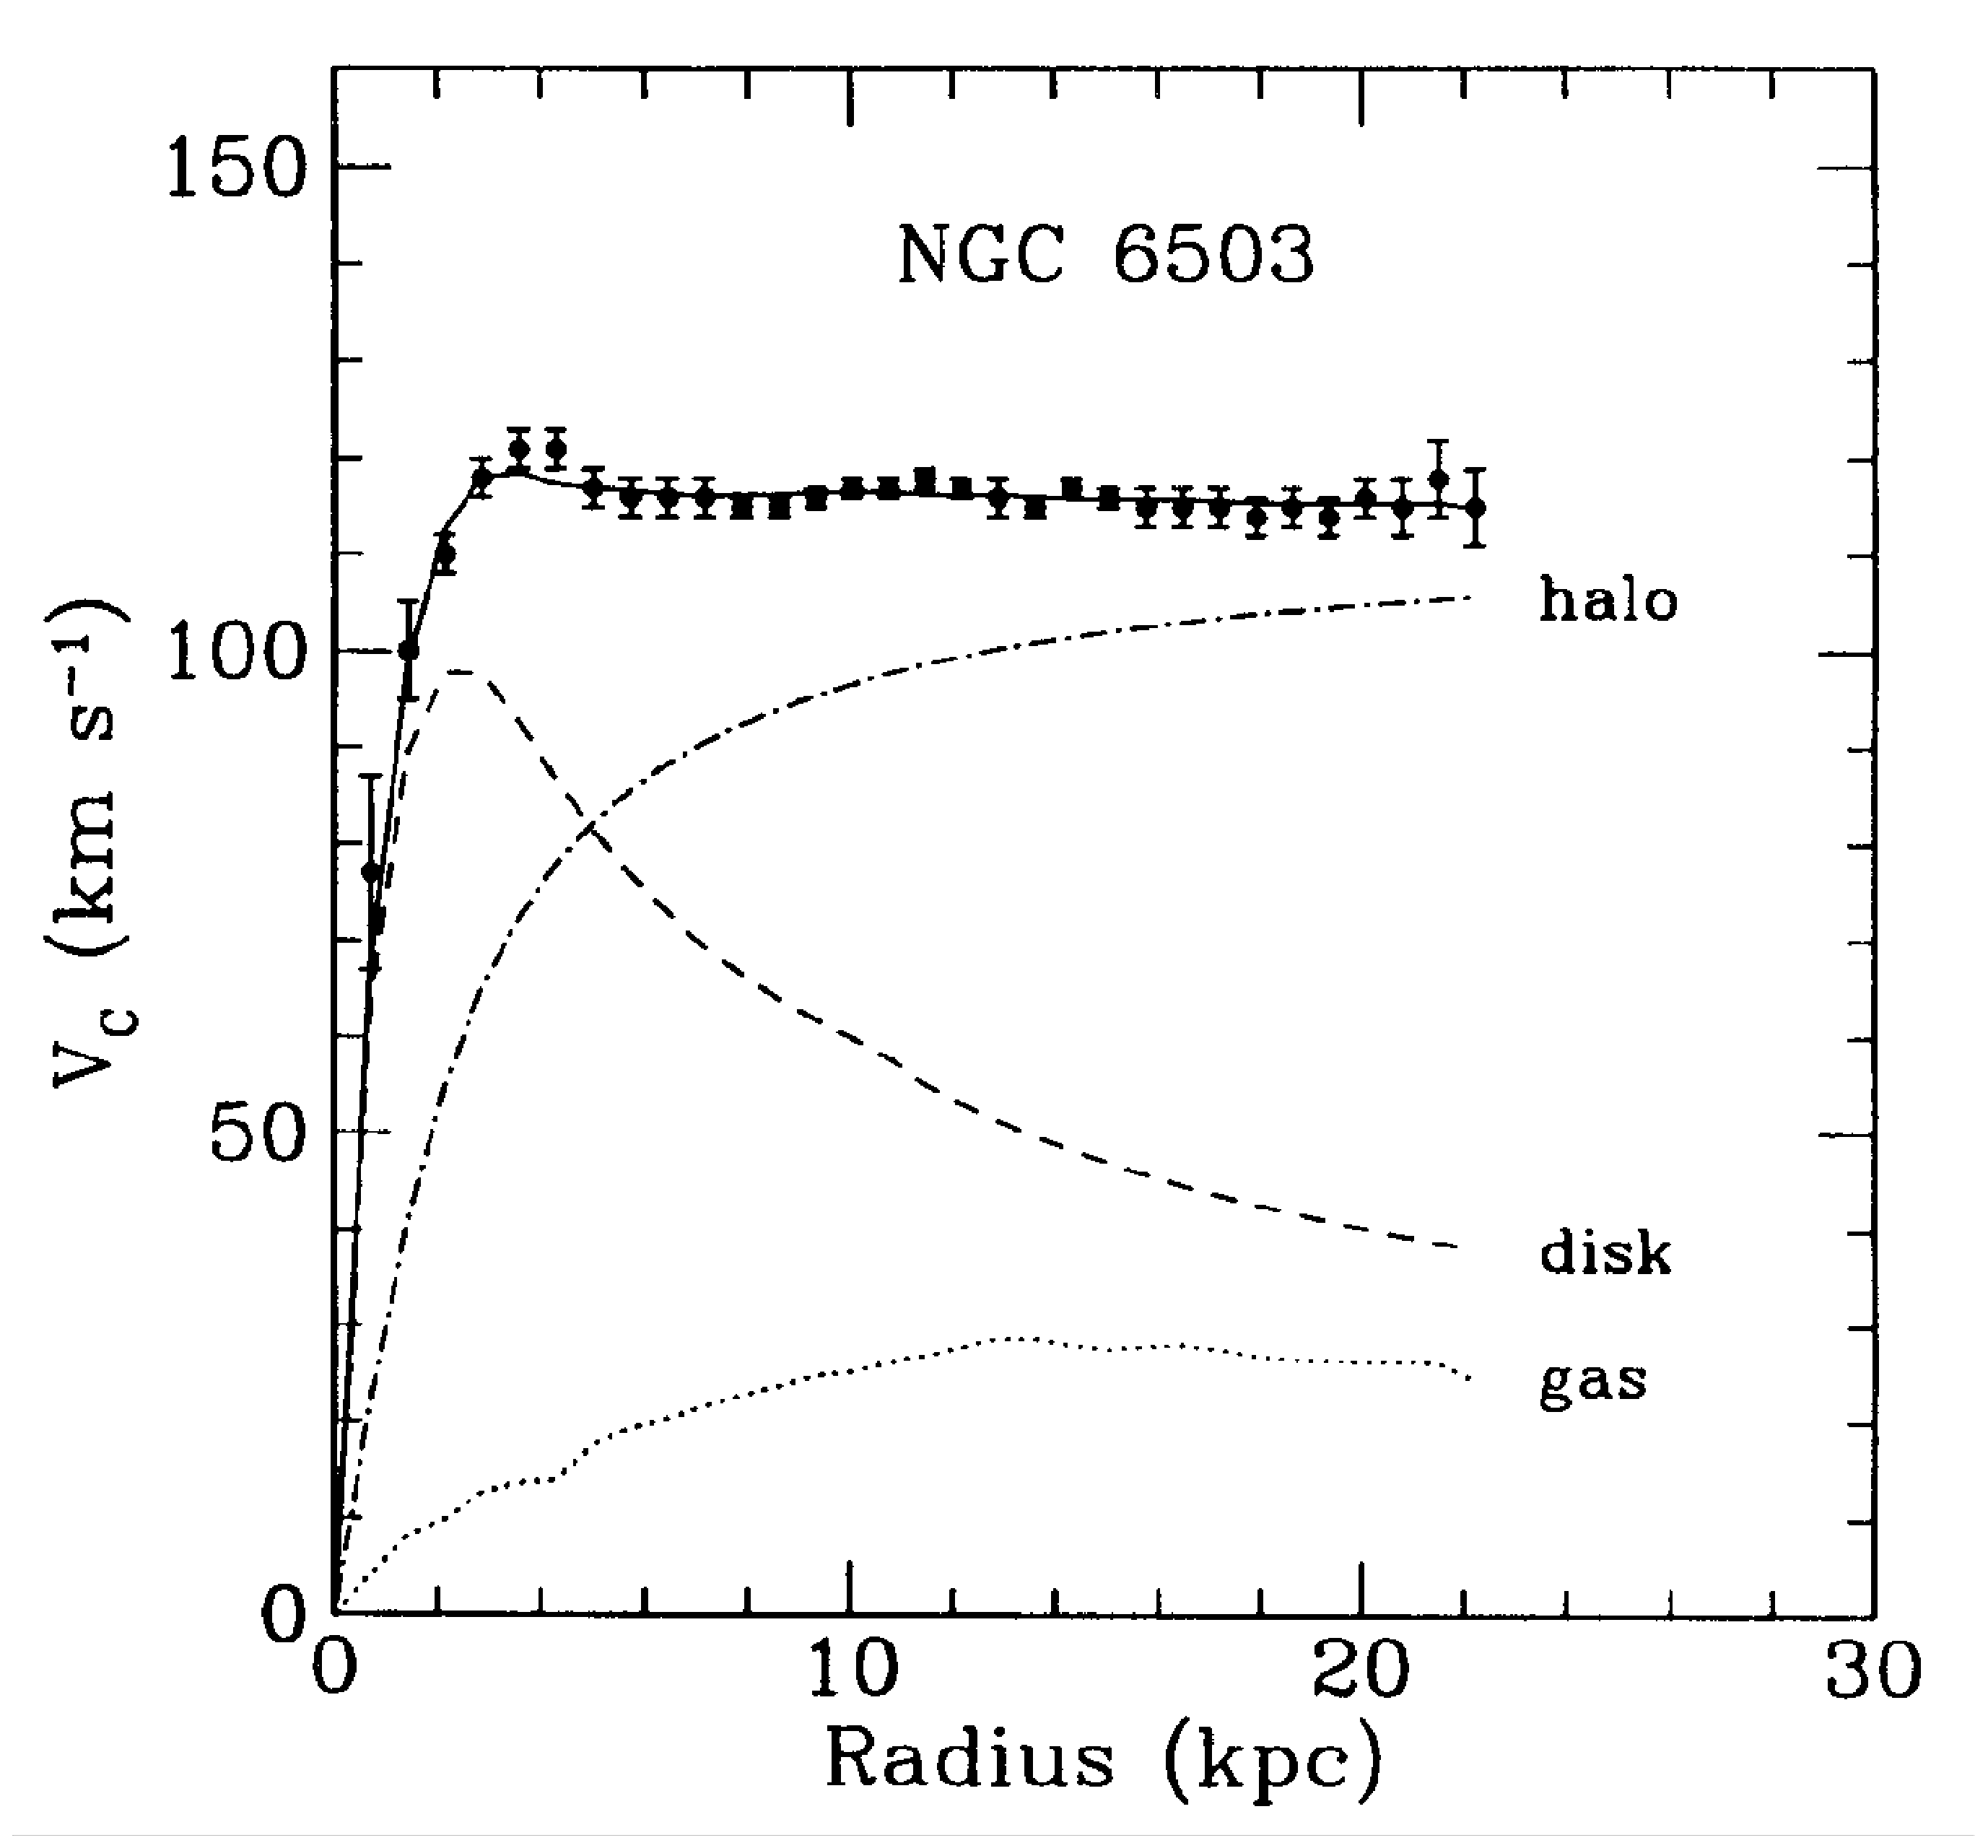
\includegraphics[width=0.7\textwidth]{Figures/Intro/rotation_curves.eps}
    \caption{Rotation curve of NGC 6503~\cite{1991MNRAS.249..523B}. The disk and gas components fail to explain the flat rotataion curve at large radii. A dark matter halo component is needed.}
    \label{fig:rotation_curves}
\end{figure}

\subsection{Gravitational lensing and the Bullet Cluster}

Gravitational field bends the trajectory of light, according to general relativity. In the Universe, the inhomogeneous gravitation field will bend the lights from distant objects such as galaxies during their propagation to the Earth. The images of the distant galaxies observed by us will therefore be distorted. This effect is called gravitational lensing. Weak gravitational lensing of distant galaxies by foreground structures has provided a direct measure of the matter distribution in the Universe~\cite{2002NewAR..46..767H}. Based on weak lensing measurements,  the Sloan Digital Sky Survey finds that dark matter is required to explain the masses and sizes of many galaxies~\cite{2006ApJS..162...38A}.

Another direct proof of the existence of dark matter comes from weak lensing observations of the ``Bullet Cluster''~\cite{2006ApJ...648L.109C}. The Bullet Cluster, or 1E 0657-558, shows the merging of two clusters at $z=0.296$. Figure~\ref{fig:bullet} shows the X-ray image of the cluster that traces the stellar component of the cluster. However, the week lensing map that traces the gravitational potential does not overlap with the X-ray image. Therefore, the dominant mass of the cluster is non-baryonic. Thus, the Bullet Cluster provides direct proof of dark matter.

\begin{figure}[htb]
    \centering
    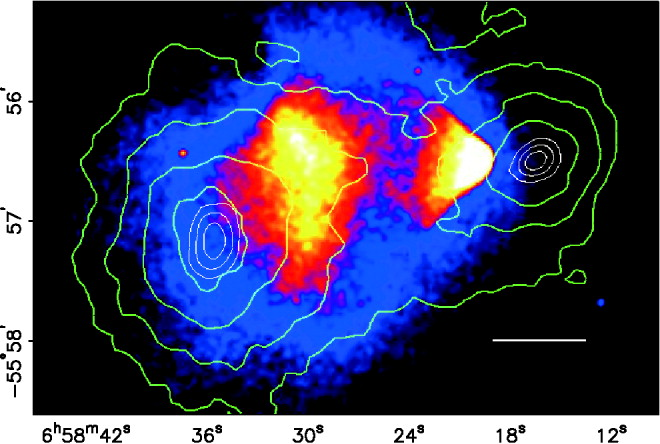
\includegraphics[width=0.7\textwidth]{Figures/Intro/bullet.jpg}
    \caption{\textit{Chandra} X-ray image of the cluster~\cite{2006ApJ...648L.109C}.  On top of it, the green contours show the week lensing that traces the gravitational potential of the cluster. }
    \label{fig:bullet}
\end{figure}

\subsection{Cosmological microwave background}

The Cosmological Microwave Background (CMB) is the remnant radiation from the epoch of the ``recombination'' of electrons and protons, which happens at a redshift $z = 1100$~\cite{2003moco.book.....D}. The measured CMB is a black body radiation with an average temperature $T = 2.725$K. It is extremely uniform across the sky, with temperature fluctuations at the level of $10^{-5}$~\cite{2002ARA&A..40..171H}. 

The power spectrum of the CMB anisotropies is a powerful probe of cosmological parameters. It is common to expand the temperature fluctuations of the CMB in spherical harmonics,
\begin{equation}
    \Theta(\hat{\bm n}) = \frac{\delta T}{T}(\hat{\bm n}) = \sum^{l=\infty}_{l=0}\sum^{m=l}_{m=-l} \Theta_{lm}Y_{lm}(\hat{\bm n}).
\end{equation}
The power spectrum $C_l$ describes the ensemble average of the fluctuations,
\begin{equation}
    \delta_{ll'}\delta_{mm'}C_l = \langle\Theta_{lm}\Theta^*_{l'm'}\rangle,
\end{equation}
which is often plotted in the scale-invariant way,
\begin{equation}
    D_l = \frac{l(l+1)}{2\pi}C_l.
\end{equation}

Figure~\ref{fig:cmb} shows the measured CMB power spectrum $D_l$ as a function of the multipoles $l$ by the European Space Agency's \emph{Planck} satellite~\cite{2020A&A...641A...6P}. The relative height of the peaks in the CMB power spectrum has information such as the curvature, the matter fraction, and the dark matter fraction of the Universe. The best-fit cosmological model of Planck reads the matter fraction $\Omega_m = 0.316$ and the dark matter fraction $\Omega_\mathrm{DM} = 0.265$. The remaining energy budget of the Universe is filled by the dark energy ($\Omega_\Lambda = 0.684$). Therefore, more than 80\% of the matter in the Universe is in the form of dark matter. The CMB measurement provides the most accurate estimate of the dark matter component in the Universe.
\begin{figure}[htb]
    \centering
    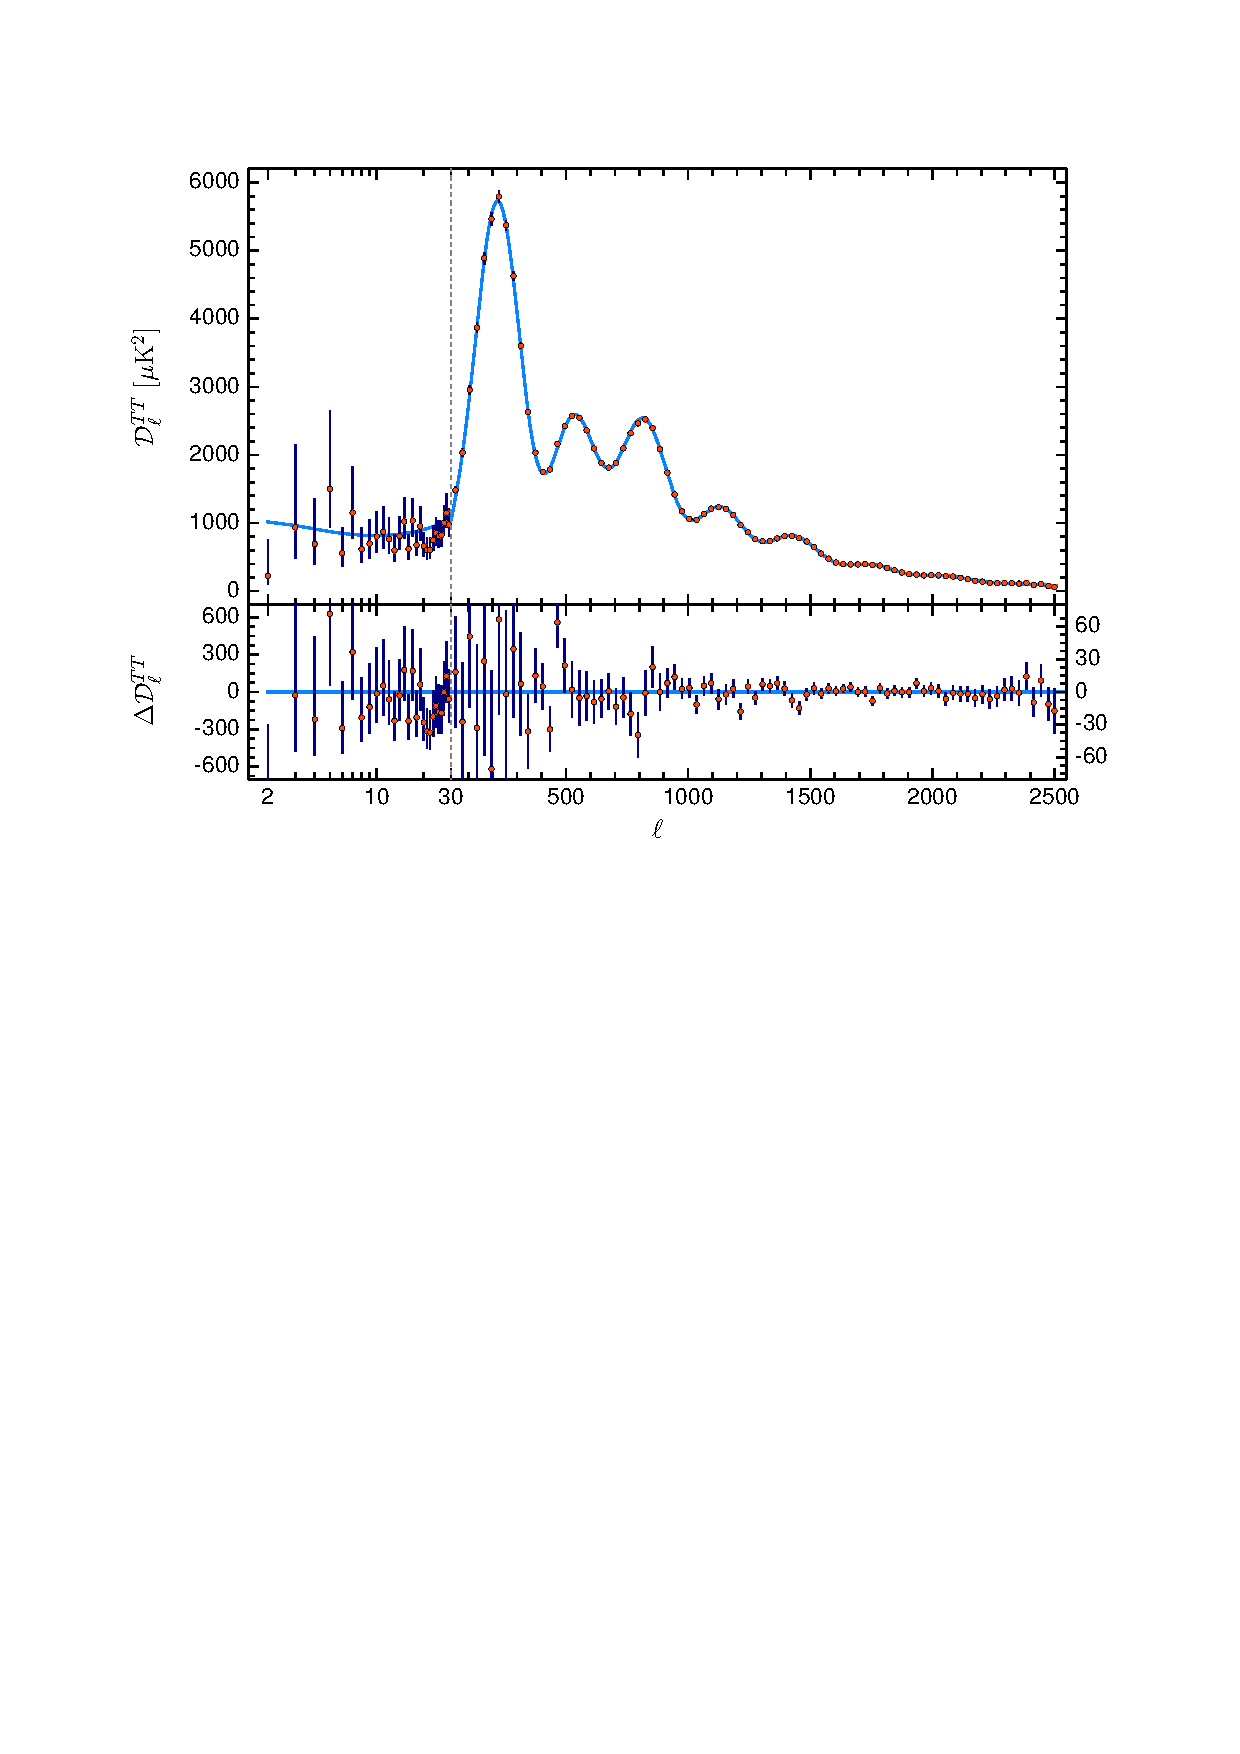
\includegraphics[width=\textwidth]{Figures/Intro/Planck_CMB.pdf}
    \caption{CMB power spectrum measured by \emph{Planck} satellite~\cite{2020A&A...641A...6P}. The locations and heights of the peaks encode the cosmological parameters of our Universe.}
    \label{fig:cmb}
\end{figure}

\section{The WIMP model}\label{se:wimp}

\begin{figure}[htb]
    \centering
    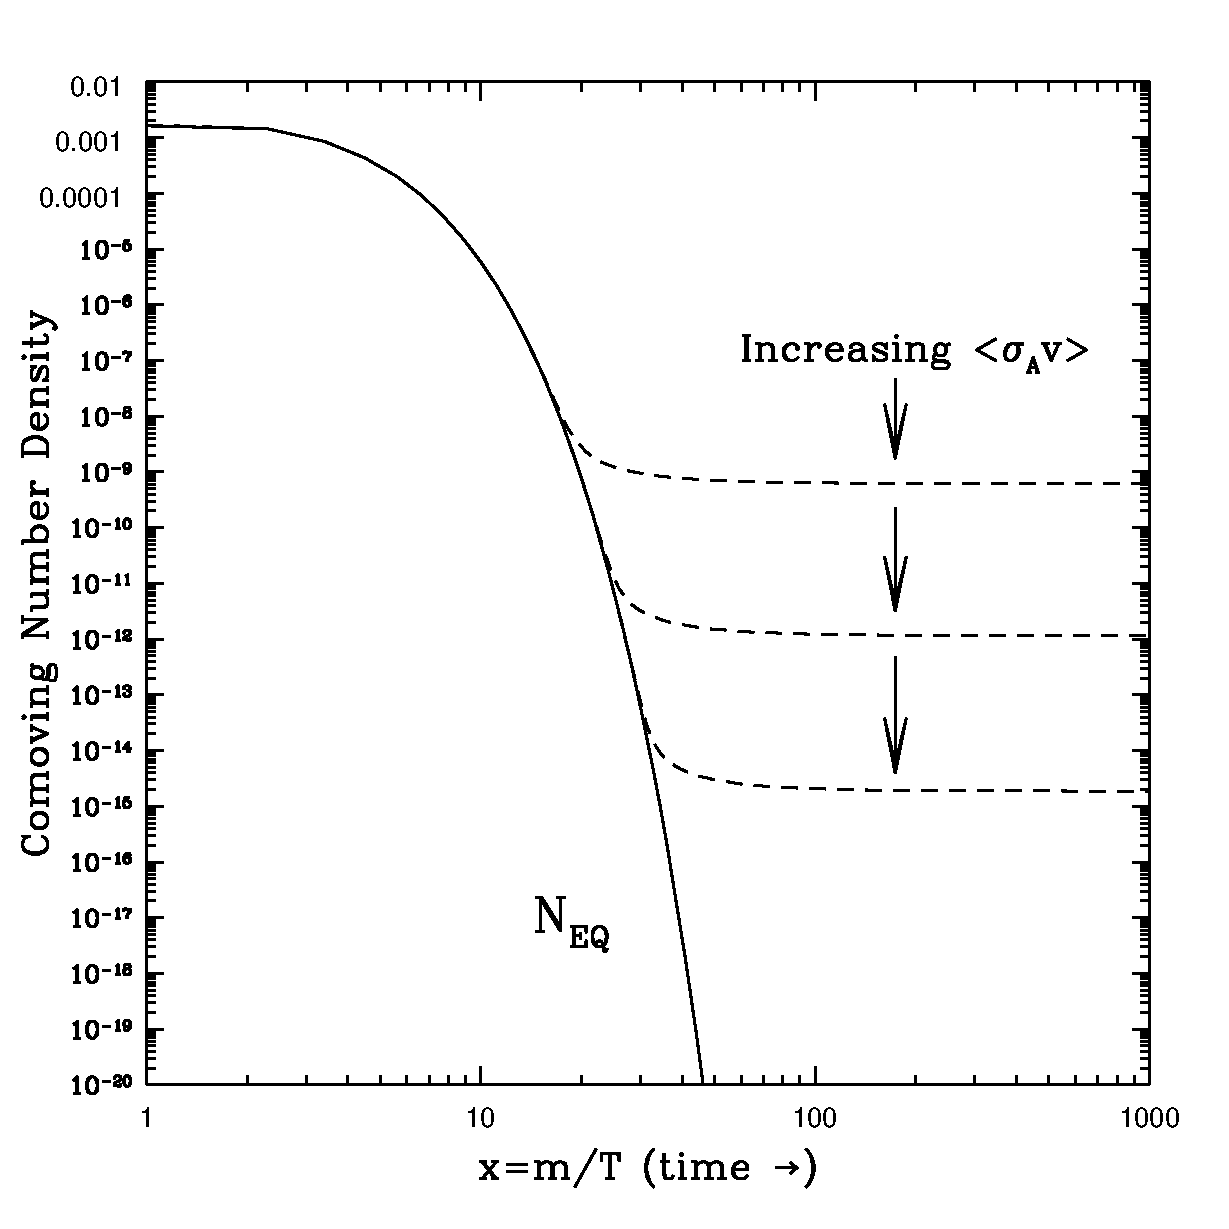
\includegraphics[width=0.7\textwidth]{Figures/Intro/freezeout.ps}
    \caption{The freeze-out of dark matter in the early Universe~\cite{2009arXiv0901.4090H}. The solid curve is the equilibrium number density. The dashed curves show the dark matter number density after it falls out of equilibrium (the relic number density).}
    \label{fig:freeze-out}
\end{figure}

The CMB observation means that dark matter is not made out of missing baryon matter. In the meantime, the SM cannot provide any viable dark matter candidate. A new type of particles beyond the SM is needed.  Many candidates have been proposed to solve the dark matter problem~\cite{2005PhR...405..279B}. Among them, the WIMP model is one of the highly motivated models. Ref.~\cite{1979ARNPS..29..313S} shows that a new particle with a weak scale mass and interaction cross section can naturally generate the current average energy density of dark matter in the Universe. This section reviews this scenario, which is often called the ``freeze-out'' of WIMP dark matter.

The Boltzmann equation for the number density of the dark matter particles in the early Universe is given by
\begin{equation}
    \frac{dn_\chi}{dt} + 3Hn_\chi = \langle\sigma v\rangle(n_\chi^{\mathrm{eq}} - n_\chi).
\end{equation}
Here $\langle\sigma v\rangle$ is the thermal-average cross section of dark matter. On the right hand side of the Boltzmann equation, we need the first term for the production of dark matter from SM particles, and the second term for the dark matter annihilation. $n_\chi^{\mathrm{eq}}$ is the number density at thermal equilibrium. For massive particles in the Maxwell-Boltzmann approximation,
\begin{equation}
    n_\chi^{\mathrm{eq}} = g\left( \frac{m_\chi T}{2\pi} \right)^{3/2}\exp(-m_\chi/T).
\end{equation}
There are two limits of the Boltzmann equation. At high temperatures $T \gg m_\chi$, dark matter is in equilibrium, $n_\chi = n_\chi^{\mathrm{eq}}$. In the other limit $T \ll m_\chi$, $n_\chi^{\mathrm{eq}}$ is suppressed by the exponential term, $\exp(-m_\chi/T)$. The production of dark matter $\langle\sigma v\rangle n_\chi^{\mathrm{eq}}$ is negligible. Thus, the number density of dark matter $n_\chi$ drains rapidly because of the Hubble expansion and the annihilation. The freeze-out of dark matter happens when the annihilation is comparable to the expansion rate of the Universe,
\begin{equation}
    \langle\sigma v\rangle n_\chi \sim H.
\end{equation}
The Hubble rate $H = 1.66\sqrt{g_*(T)}/M_{pl}$, where $M_{pl} \approx 1.22\times 10^{19}$ GeV is the Planck mass. The effective number of degree of freedom,
\begin{equation}
    g_*(T) = \sum_{i=b}g_i\left(\frac{T_i}{T}\right)^4 + \sum_{i=f}\frac{7}{8}g_i\left(\frac{T_i}{T}\right)^4
\end{equation}
counts the relativistic degree of freedom at the temperature $T$. Here $g_i$'s are the internal degrees of freedom of the particle species,  and $T_i$'s are the temperatures of the decoupled particles.

The number density of dark matter at the freeze-out temperature $T_f$ is therefore,
\begin{equation}
    \left.n_\chi\right|_{T = T_f} \approx \left.\frac{H}{\langle\sigma v\rangle}\right|_{T = T_f} \approx \frac{1.66\sqrt{g_*(T_f)}T_f^2}{\langle\sigma v\rangle M_{pl}}.
\end{equation}
The relic abundance of dark matter today ($T=T_\mathrm{CMB}$) is
\begin{equation}
    \Omega_\mathrm{DM} = \frac{\rho_\mathrm{DM}}{\rho_c} = \frac{\left. m_\chi n_\chi\right|_{T = T_f}}{\rho_c}\frac{s(T_\mathrm{CMB})}{s(T_f)}.
\end{equation}
The entropy density\footnote{The effective number of degrees of freedom in entropy $g_{*,S}(T)$ is different from the $g_{*}(T)$ as
\begin{equation*}
    g_{*,S}(T) = \sum_{i=b}g_i\left(\frac{T_i}{T}\right)^3 + \sum_{i=f}\frac{7}{8}g_i\left(\frac{T_i}{T}\right)^3.
\end{equation*}
} $s(T) = (2\pi/45)g_{*,S}(T)T^3$ scales with $1/a^3$. For dark matter with a weak scale mass, the freeze-out temperature $T_f \sim m_\chi/25$. One can estimate the relic abundance of dark matter,
\begin{equation}
    \Omega_\mathrm{DM} \approx 0.26 \left( \frac{m_X}{100\ \mathrm{GeV}} \right) \left( \frac{2.2\times 10^{-26}\ \mathrm{cm}^3\ \mathrm{s}^{-1}}{\langle\sigma v\rangle} \right).
\end{equation}
In the estimate, we use $g_{*,S}(T_\mathrm{CMB}) = 3.909$ and $g_{*,S}(T_f) = g_{*}(T_f) = 86.25$~\cite{2016Galax...4...78H}. The value $\langle\sigma v\rangle = 2.2\times 10^{-26}\ \mathrm{cm}^3\ \mathrm{s}^{-1}$ is the minimum cross section to avoid an overabundance of dark matter , and is a often-used benchmark for dark matter indirect detection.

The WIMP model is especially favored because many particle theories naturally provide candidates for the weak scale particle that can explain the dark matter relic abundance. For example, the lightest \textit{neutralino} in the supersymmetric theory, or the Kaluza-Klein states in models of extra dimensions, are all motivated by particle physics problems~\cite{2005PhR...405..279B}. The fact that cosmology implies them as viable dark matter candidates is called the ``WIMP miracle''. Although many assumptions are made for the ``miracle'' to work~\cite{2019arXiv190407915L}, this remarkable coincidence between particle physics and cosmology still motivate the weak scale as a very promising scale for new physics, and many efforts have been devoted to the search of WIMPs.

\section{Searching for dark matter}

A pedagogical Feynman diagram is often used (Fig.~\ref{fig:dm_search}, from Ref.~\cite{2019FrP.....7...75G}) to illustrate three dark matter detection channels: direct detection, collider production, and indirect detection. We review them in this section.

\begin{figure}[htb]
    \centering
    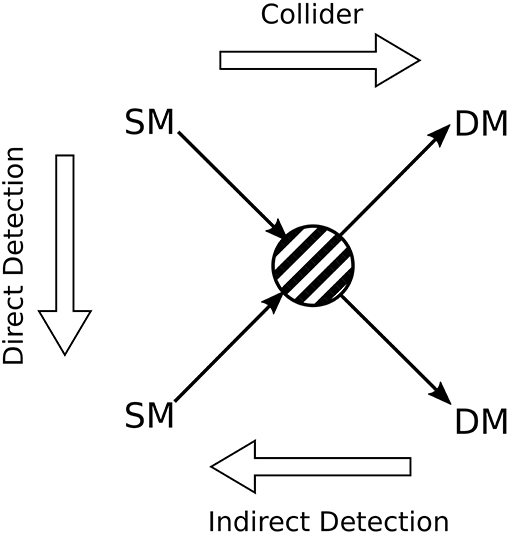
\includegraphics[width=0.7\textwidth]{Figures/Intro/dm_diagram.jpg}
    \caption{A pedagogical Feynman diagram for dark matter detection channels~\cite{2019FrP.....7...75G}: direct detection for SM particles interacting with dark matter; collider production for SM particles colliding and producing dark matter; indirect detection for dark matter annihilation or decay into SM particles.}
    \label{fig:dm_search}
\end{figure}

\subsection{Direct detection}

\citet{1985PhRvD..31.3059G} first proposed the idea of direct detection for WIMP dark matter. In direct detection, the dark matter particles can elastically scatter off nuclei, transferring energy to the recoiling nuclei. The recoil energy spectrum induced by dark matter can be measured when the kinetic energy of the up-scattered electron is released in ionization and scintillation. 

The differential rate for dark matter-nuclei scattering is
\begin{equation}
    \frac{dR}{dE_R} = N_N\frac{\rho_0}{m_\mathrm{DM}}\int_{v_\mathrm{min}}^{v_\mathrm{max}}d\bm{v}f(\bm{v})v\frac{d\sigma}{dE_R},
\end{equation}
where $N_N$ is the number of the nuclei, $\rho_0$ is the local dark matter density at the location of the Earth, $f(\bm{v})$ is the dark matter velocity distribution function, and $d\sigma/dE_R$ is differential cross section for dark matter-nuclei scattering.

The local dark matter density and velocity distribution are needed as inputs to infer the dark matter-nuclei scattering cross section. However, those values depend on the astrophysical measurement and have uncertainties. The local dark matter density can vary from 0.2 to 0.4 GeV cm$^{-3}$~\cite{2010A&A...509A..25W}. In the so-called standard halo model that assumes smooth phase-space distribution of dark matter, the velocity distribution function is Maxwellian,
\begin{equation}
    f(v) = \frac{1}{\sqrt{2\pi \sigma_c}}\exp\left(-\frac{v^2}{2\sigma_c^2}\right)
\end{equation}
where $\sigma_c \approx 270$ km s$^{-1}$~\cite{2012PDU.....1...94B}. However, the standard halo model has been challenged by the recent Gaia observation: the more realistic dark matter velocity distribution is affected by dark matter substructures near the Solar neighborhood~\cite{2019ApJ...874....3N}. 

Noble liquid detectors in underground laboratories are standard detector designs for direct detection for low background and large target mass~\cite{2012PDU.....1...94B}. Current experiments like the XENON1T~\cite{2019PhRvL.122g1301A} have been operating with target nuclei mass at the level of hundreds of kilograms and are probing deeply in the parameter space of dark matter-nucleus interaction.

\subsection{Collider search}

Dark matter particles may be produced at high-energy particle colliders such as the Large Hadron Collider~\cite{2013IJMPA..2830052M}. Dark matter would be invisible to the detectors at the collider, but its production can be identified by looking at the SM particles associated with dark matter. Conservation of energy and momentum can be applied to construct the missing energy and momentum of dark matter. Unlike direct detection, the collider search of dark matter is independent of the local dark matter density and velocity distribution, to which astrophysical uncertainties apply.

\subsection{Indirect detection}\label{sse:indirect}

In indirect detection, dark matter particles will annihilate or decay into SM particles. When that happens on the galactic or cosmological scale, the large number of astrophysical observations on the Earth may have chances to detect the SM products of dark matter annihilation or decay. Although the interaction rates between dark matter and SM particles are expected to be weak, a large amount of dark matter present in the Universe may still cause detectable signals on the Earth.

Gamma rays and neutrinos travel to us in straight lines. In the case of annihilation, the differential flux from dark matter in the cosmos is,
\begin{equation}\label{eq:ann}
    \frac{dN}{dEdt} = \frac{1}{8\pi}\frac{dN_\gamma}{dE_\gamma}\frac{\sigmav}{m_\mathrm{DM}^2}\int_{los}\int_{d\Omega}\rho^2(l,\Omega)dld\Omega.
\end{equation}
Here, $dN_\gamma/dE_\gamma$ is the annihilation spectrum of dark matter. The integral over the solid angle and the line-of-sight (los) is called the J-factor of dark matter annihilation,
\begin{equation}\label{eq:jfactor}
    J_\mathrm{ann} = \int_{los}\int_{d\Omega}\rho^2(l,\Omega)dld\Omega.
\end{equation}
The dark matter density $\rho(l,\Omega)$ is squared to account for the annihilation. The J-factor is a measure of the expected dark matter signal from the region of observation.

One of the most interesting regions to search for dark matter annihilation is the Galactic center. In Sec.~\ref{sse:rotation_curve}, we have shown that the dark matter density $\rho \sim 1/r^2$ at large radii to explain the flat rotation curve. However, rotation curve measurements are uncertain and only weakly constrain the dark matter density at small radii, especially for the Milky Way. The N-body simulation is a commonly used approach to study the dark matter distribution at different scales. Based on N-body simulations, the Navarro-Frenk-White profile~\cite{1996ApJ...462..563N} suggests a universal dark matter profile of the following form,
\begin{equation}
    \rho(r) = \frac{\rho_0}{(\frac{r}{R_s})(1+\frac{r}{R_s})^2},
\end{equation}
where the scale radius $R_s$ varies from galaxy to galaxy. The dark matter density peaks as $\rho \sim 1/r$ toward the Galactic center, making it the brightest region to search for dark matter annihilation. In the next chapter, we discuss the gamma-ray excess toward the Galactic center detected by the \textit{Fermi} Large Area Telescope and its implication for dark matter annihilation.

Dark matter annihilation can also produce charged particles. The charged particles diffuse in the Galactic magnetic field as cosmic rays, losing their energies and directional information. The local density of the cosmic rays produced by dark matter can be calculated by solving the propagation of cosmic rays,
\begin{equation}
    \frac{\partial\psi}{\partial t} = q(\vec{r},E,t) + D(E)\nabla^2\psi + \frac{\partial}{\partial E}(\dot{E}\psi),
\end{equation}
where $q(\vec{r},E,t)$ is the source term of cosmic rays, $D(E)$ is the diffusion coefficient and $\dot{E}$ is the energy loss of the cosmic rays. Public tools has been developed by the community to numerically solve the propagation of cosmic rays. Examples include \textsc{dragon}~\cite{2010APh....34..274D} and \textsc{galprop}~\cite{1998ApJ...509..212S}.

The AMS-02 experiment has been measuring various species of cosmic rays arriving on the Earth from the Universe. The AMS-02 has detected a significant positron excess~\cite{2014PhRvL.113l1101A} above $\sim$ 200 GeV. The excess has been explored as an annihilation signal from WIMP dark matter of mass $\sim$ TeV, but the $\sigmav$ needed to explain the positron flux is much larger than the thermal relic cross section. More likely, the positron excess can be explained by the nearby pulsars~\cite{2009JCAP...01..025H}. A less significant anti-proton excess is also recently claimed~\cite{2017PhRvL.118s1101C}. However, the robustness of the signal needs further investigations~\cite{2019PhRvD..99j3026C, 2021arXiv210714606H}.


\chapter{Galactic center excess} \label{ch:GCE}

The \emph{Fermi} Large Area Telescope has discovered a gamma-ray excess toward the center of Milky Way. The signal, often referred as the Galactic center excess (GCE), was first identified by \citet{2009arXiv0910.2998G}, and further confirmed by many collaborations~\cite{2009arXiv0912.3828V,2011PhLB..697..412H,2012PhRvD..86h3511A,2013PhRvD..88h3521G,2014PhRvD..89f3515M,2013PDU.....2..118H,2014PhRvD..90b3526A,2016PDU....12....1D,2015JCAP...03..038C,2015PhRvD..91l3010Z,2016ApJ...819...44A,2017ApJ...840...43A}. In this chapter, we review the possible interpretations of the signal, including the dark matter scenario and the millisecond pulsar scenario. We show that understanding the morphology of the GCE is crucial for disentangling the millisecond pulsar signal from the dark matter signal.

\section{\textit{Fermi}-LAT}

The \textit{Fermi}-LAT satellite was launched by NASA on 2008, June 11. It is a pair-conversion gamma-ray telescope, covering the energy range from around 20 MeV to above 300 GeV. Figure~\ref{fig:lat}~\cite{2009ApJ...697.1071A} shows the schematic diagram of the LAT. An incoming gamma ray would interact with the tungsten layers in the detector, creating a pair of electron and positron. The trajectories of the pair particles are tracked by the silicon strips, allowing the LAT to recover the direction of the gamma ray. The calorimeter at the bottom of the detector stops the electron and positron, so that it measures the total energy of the gamma ray.

As a wide field-of-view telescope, the LAT covers about 20\% of the sky at each moment. The spacecraft orbits the earth in about 96 minutes, allowing the LAT to survey the entire sky efficiently. The angular resolution of the LAT varies with the gamma-ray energy, from about 3.5$^\circ$ at 100 MeV and 0.15$^\circ$ at above 10 GeV.

\begin{figure}[htb]
    \centering
    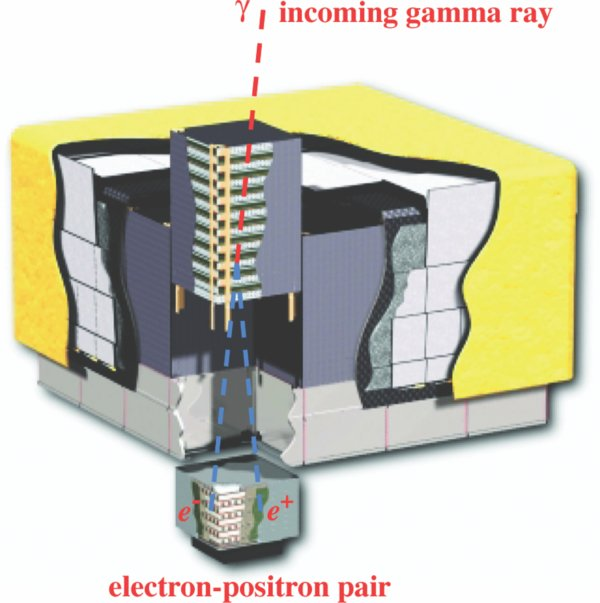
\includegraphics[width=0.7\textwidth]{Figures/Intro/lat.jpg}
    \caption{Schematic diagram of the $Fermi$-LAT~\cite{2009ApJ...697.1071A}}.
    \label{fig:lat}
\end{figure}

\section{Gamma-ray sky and the GCE}

Since its mission began, The \textit{Fermi}-LAT has discovered thousands of gamma-ray sources and revealed the large scale diffuse gamma-ray emission in the sky. Figure~\ref{fig:gamma_sky} shows the gamma-ray sky constructed by 5-year Fermi data above 1 GeV. Most remarkably, the Galactic diffuse emission dominates the central plane of the Milky Way.

\begin{figure}[htb]
    \centering
    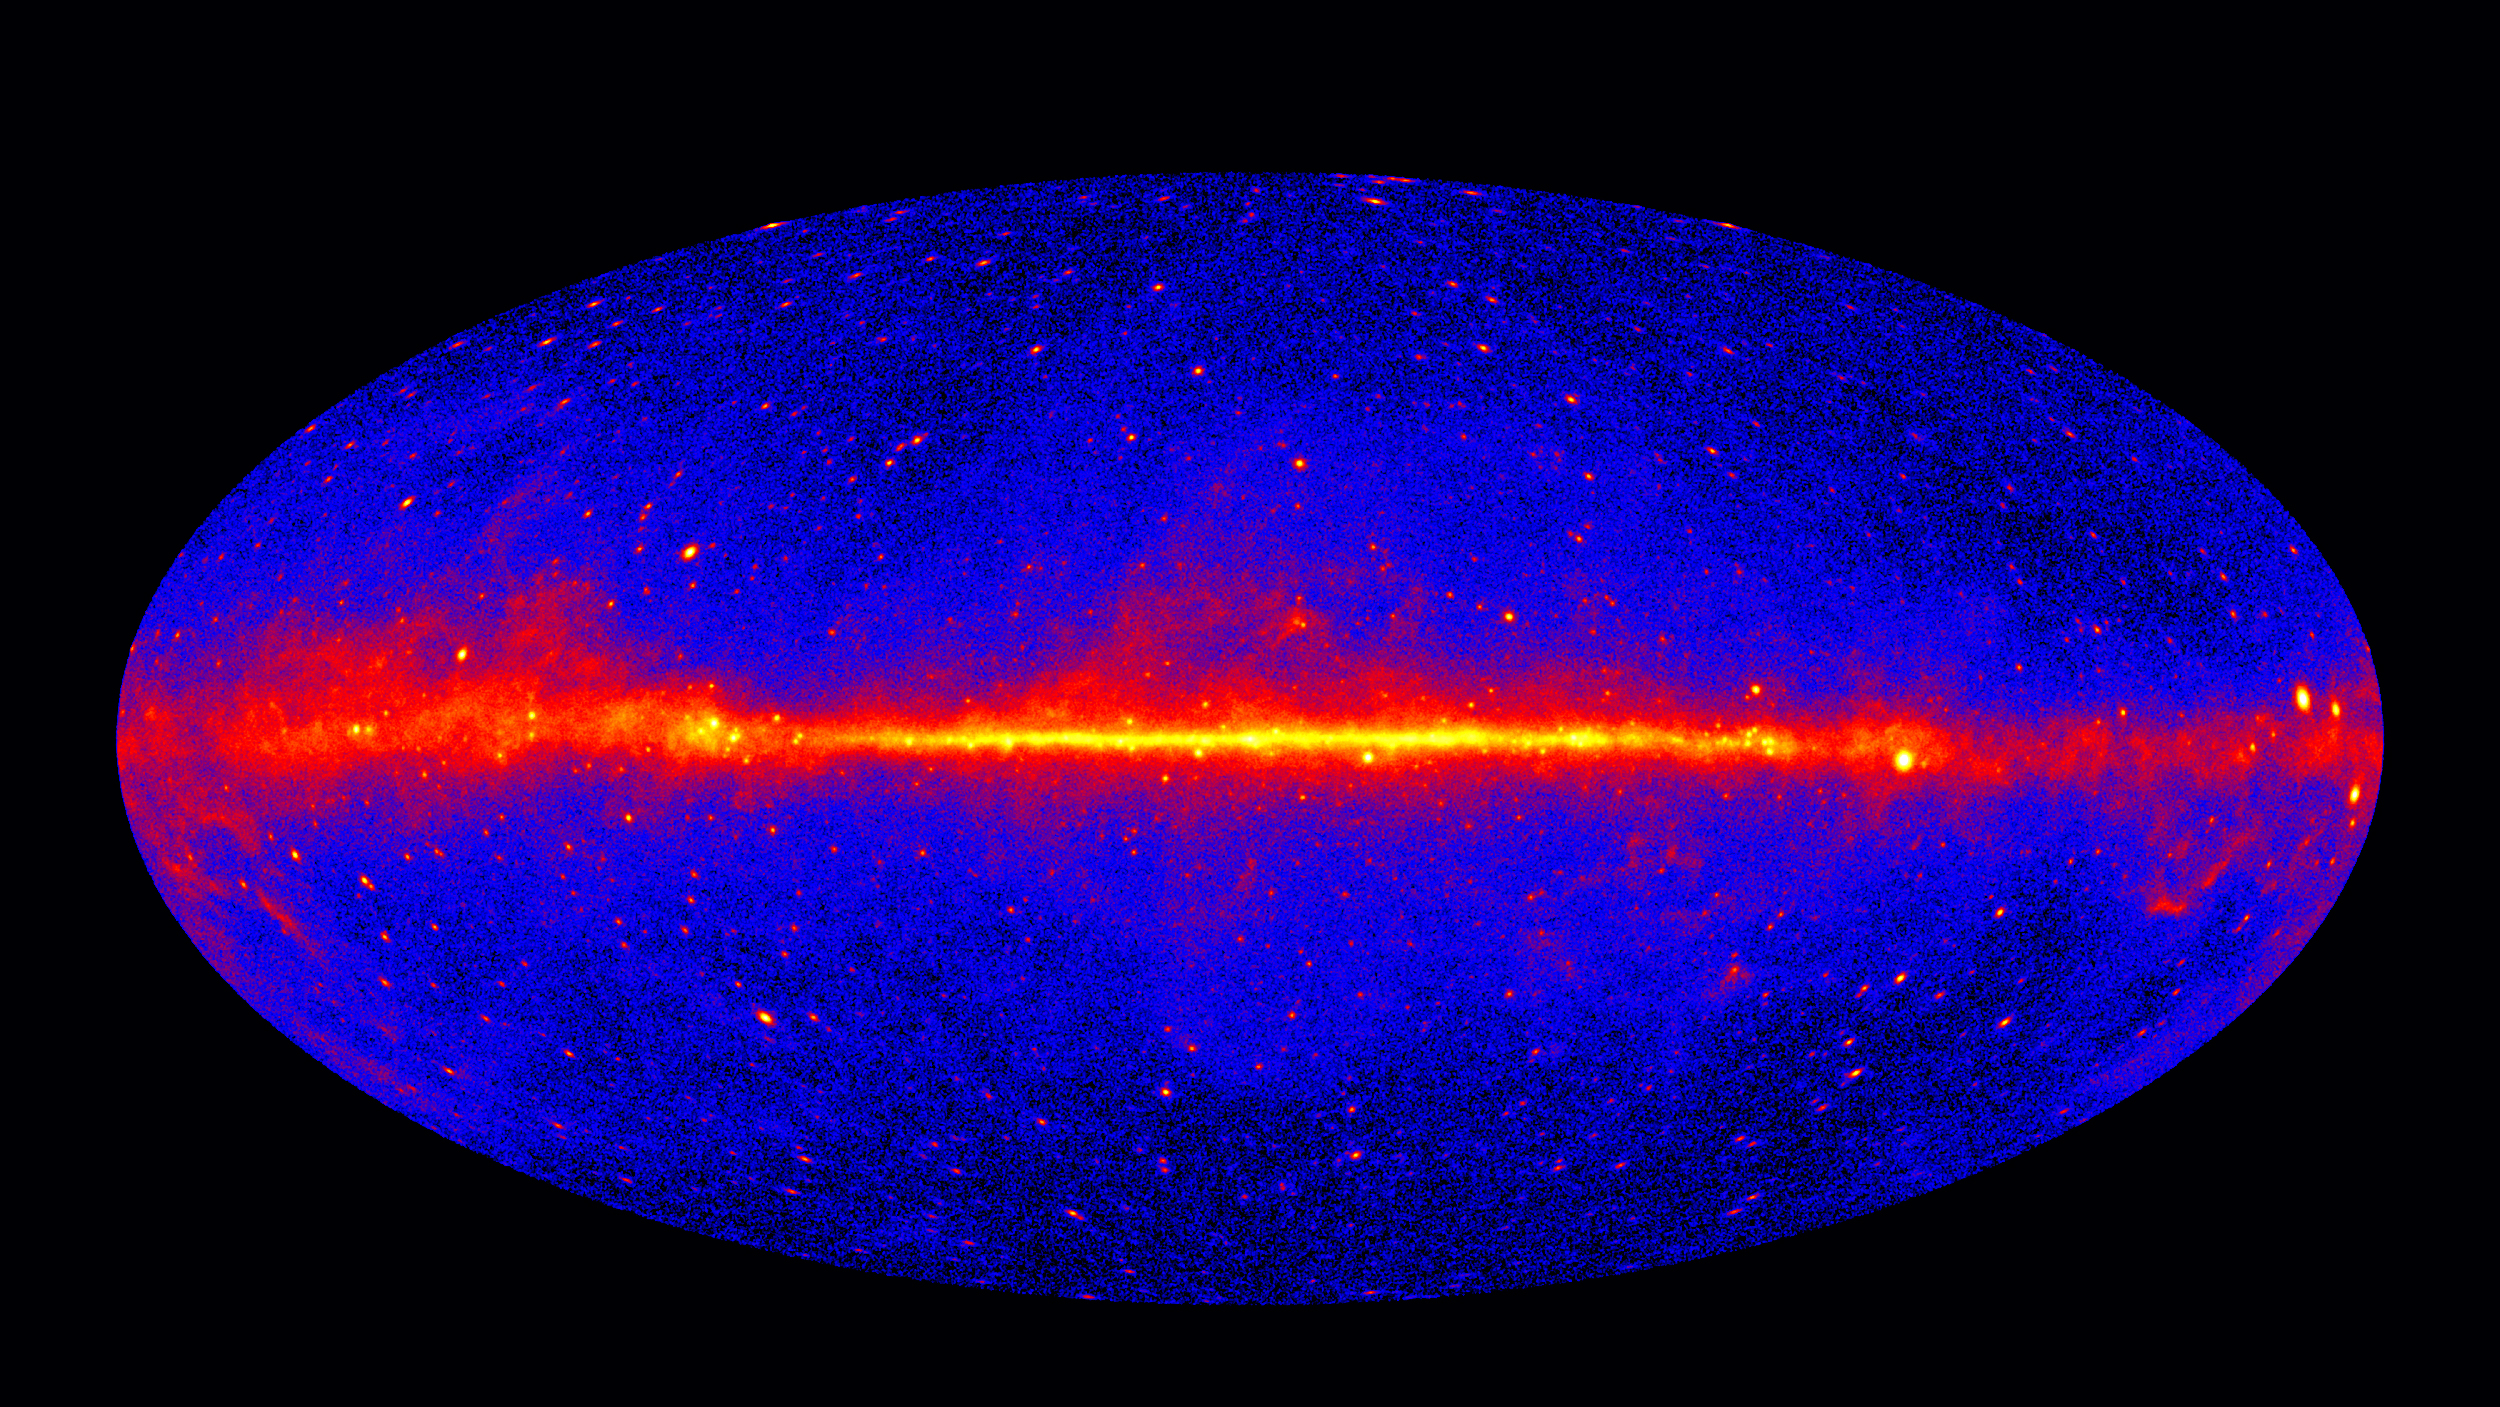
\includegraphics[width=1\textwidth]{Figures/Intro/Femri_5_year_2500x1407.jpg}
    \caption{The \textit{Fermi}-LAT 5-year gamma-ray sky for energies greater than 1 GeV~\cite{NASAs2013}. The Galactic plane is dominated by the diffuse gamma-ray emission caused by the cosmic rays interacting with the gas and radiation filed in the Milky Way.}
    \label{fig:gamma_sky}
\end{figure}
% https://svs.gsfc.nasa.gov/11342

As mentioned in Sec.~\ref{sse:indirect}, one of the most interesting regions for searching dark matter annihilation is the Galactic center. However, the rich diffuse emission in the Galactic center plays as an important background for any exotic gamma-ray signal from the same region. The template fitting technique has been developed as a standard analysis method for \textit{Fermi}-LAT data to improve the instrumental sensitivity to detect those signals. By knowing the maps of different background emissions and the expected signal in the region of interest, one can fit the data to the linear combinations of different maps (templates) and potentially detect signals below the background emission.

The Galactic diffuse emission that dominated the Galactic plane is generated by cosmic rays interacting with the  interstellar medium (gas and radiation field in the Galaxy). There are three physical processes that contributes to the Galactic diffuse emission: the  bremsstrahlung of cosmic-ray electrons with the interstellar gas; the pion production from cosmic-ray protons colliding the interstellar gas; the inverse Compton scattering of cosmic-ray electrons off the interstellar radiation field. The first two processes trace the gas maps of the Milky Way, which can be measured by the spectral line surveys of HI and CO gas. The inverse Compton scattering is determined by the cosmic-ray electrons propagation and their interaction with the interstellar radiation field (including the CMB, inferred, and starlight photons), which can be calculated with \textsc{galprop}~\cite{2017ApJ...846...67P}.

The expected gamma-ray signal from dark matter annihilation is spherically symmetric and peaks at the Galactic center, as implied by the NFW profile of dark matter.

The photon counts detected by the \textit{Fermi}-LAT from each pixel on the sky map over certain energy bin $\Delta E$ can be treated independently, therefore the likelihood function is Poissonian,
\begin{equation}
    \mathcal{L}(\mu|n)= \sum_{ij}\frac{\mu_{ij}^{n_{ij}}e^{(-\mu_{ij})}}{n_{ij}!},
\end{equation}
where $n_{ij}$ is the \textit{Fermi} data for different pixels and the model $\mu_{ij}$ is a linear combination of model templates $\Phi_{ij}$,
\begin{equation}
    \mu_{ij} = \sum_m \alpha_m \Phi^m_{ij}.
\end{equation}
For the Galactic center, the relevant background templates include the gas-correlated maps (for the bremsstrahlung and the pion decay), the inverse Compton map, the point sources in the region, and the Fermi Bubble~\cite{2010ApJ...724.1044S}.

Including the NFW profile for dark matter in the fit, a gamma-ray excess has been identified in the \textit{Fermi}-LAT data~\cite{2009arXiv0910.2998G, 2009arXiv0912.3828V,2011PhLB..697..412H,2012PhRvD..86h3511A,2013PhRvD..88h3521G,2014PhRvD..89f3515M,2013PDU.....2..118H,2014PhRvD..90b3526A,2016PDU....12....1D,2015JCAP...03..038C,2015PhRvD..91l3010Z,2016ApJ...819...44A,2017ApJ...840...43A}. The spectra of the excess depend on the background models and fitting procedures in different studies, but overall they are consistent with a spectrum that peaks at a few GeV (see Fig.~\ref{fig:gce_spectra}~\cite{Murgia:2020dzu}).
\begin{figure}[htb]
    \centering
    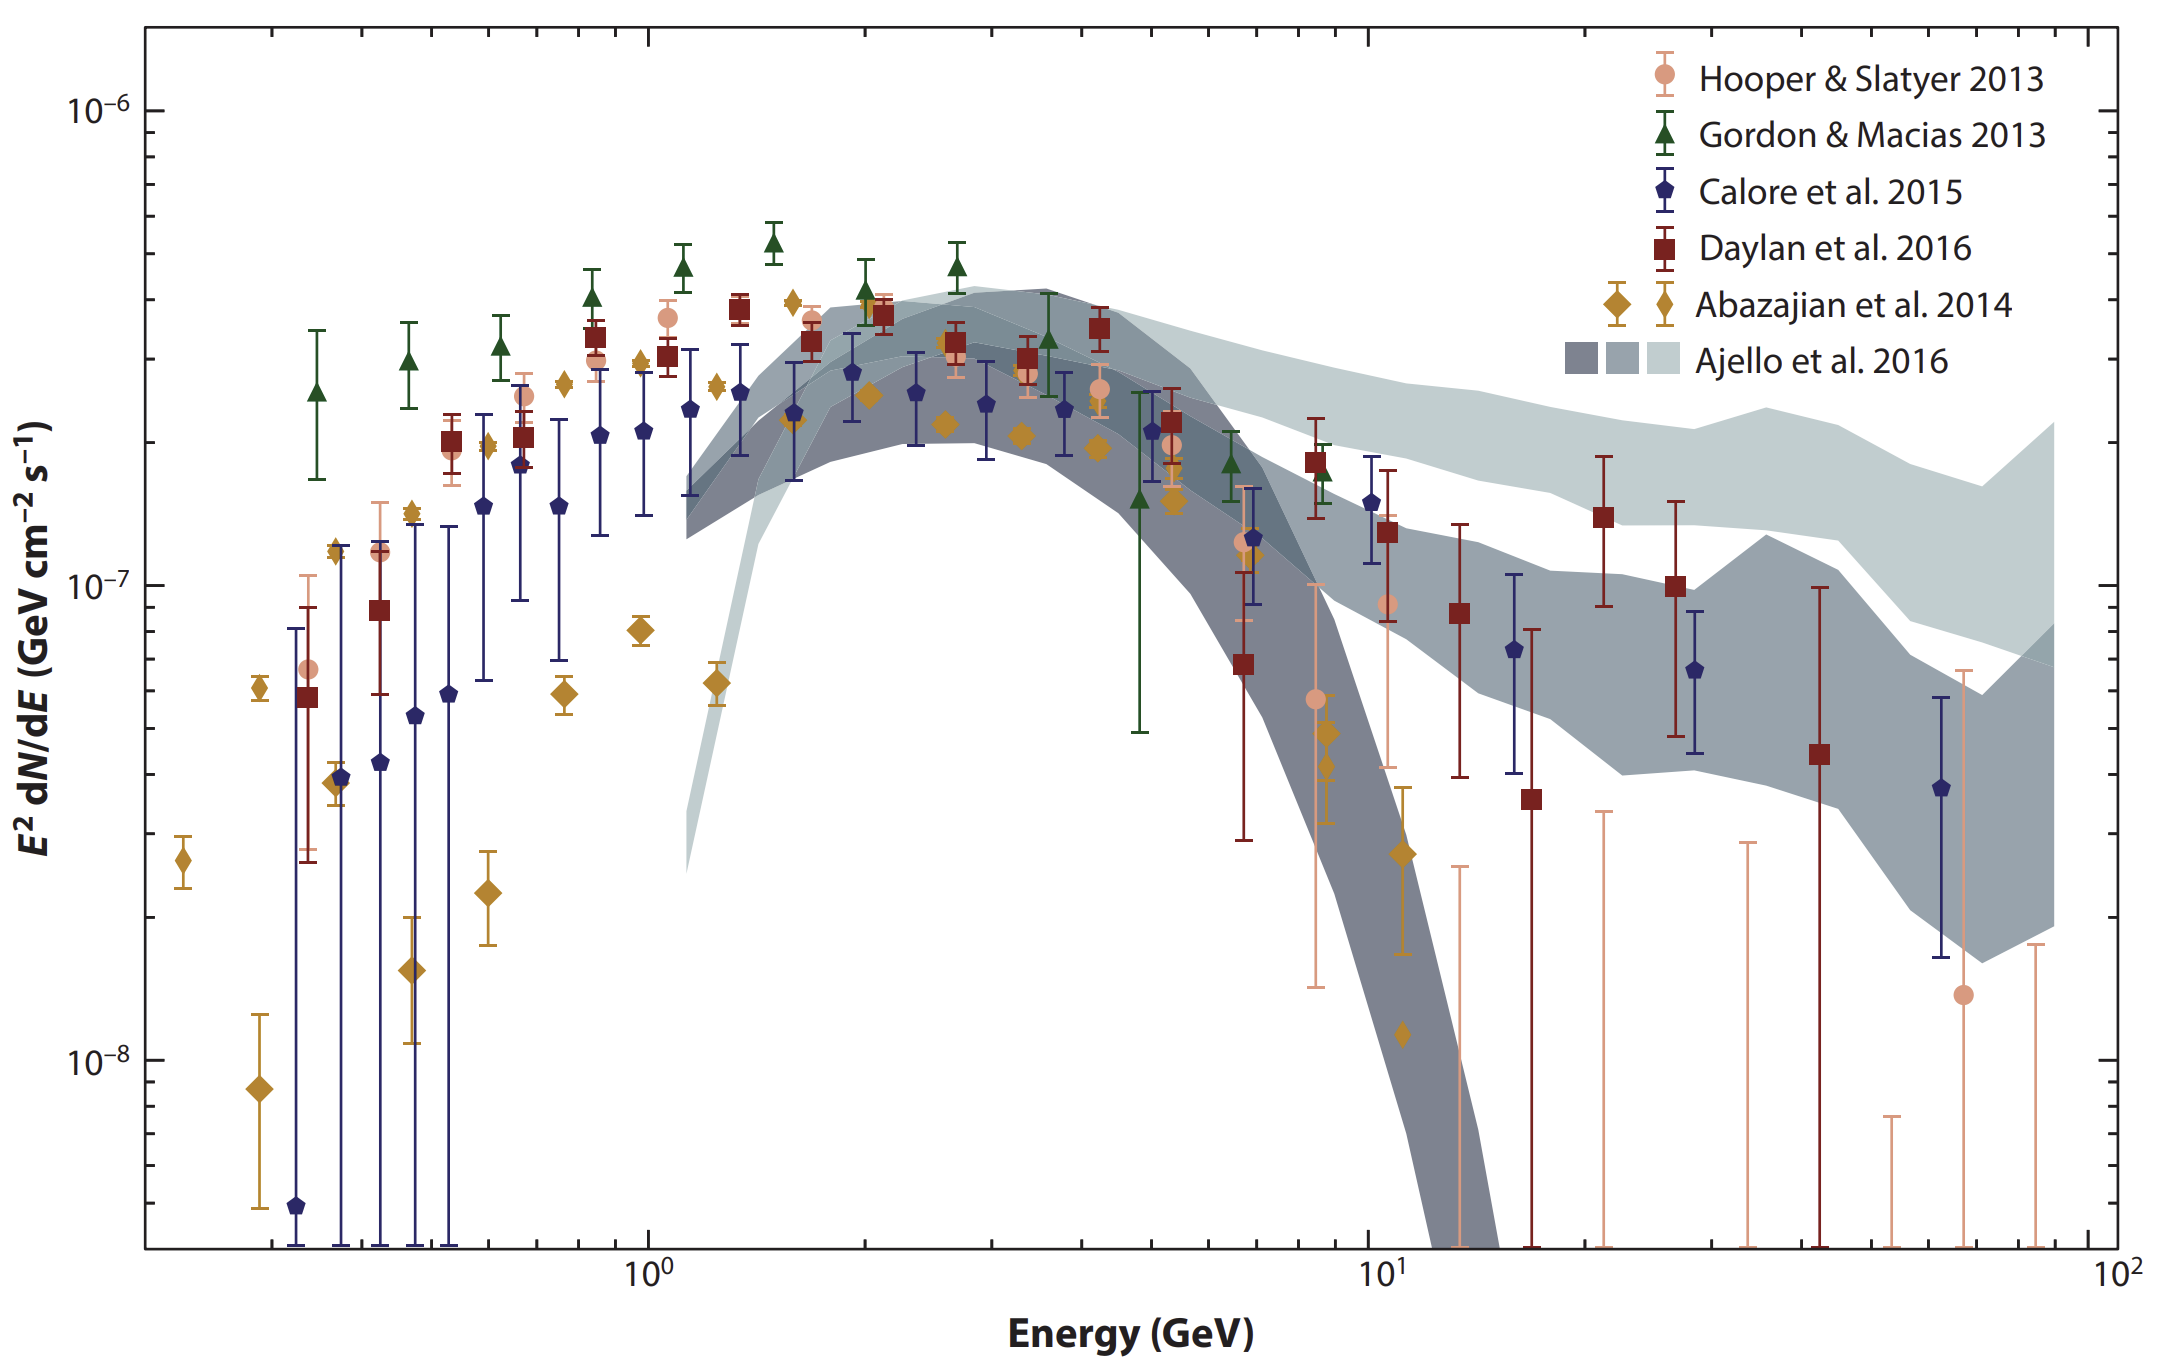
\includegraphics[width=\textwidth]{Figures/Intro/gcespectrum.png}
    \caption{GCE fluxes based on different studied~\cite{Murgia:2020dzu}. The fluxes are scaled to a $15^\circ \times 15^\circ$ region about the GC. The peak energy of $\sim 1 - 3$ GeV is a robust feature of the GCE spectrum.}
    \label{fig:gce_spectra}
\end{figure}

\subsection{Dark matter interpretation}

It has been shown that WIMP dark matter annihilation can explain the unique feature of the peaked GCE spectrum. 
%The implied $\sigmav$ of the GCE, after normalizing the NFW profile with local dark matter density, is consistent with the thermal relic cross section. 
The gamma-ray flux from dark matter annihilation, as described by Eq.~\ref{eq:ann}, is
\begin{equation}
    \frac{dN}{dEdt} = \frac{1}{8\pi}\frac{dN_\gamma}{dE_\gamma}\frac{\sigmav}{m_\mathrm{DM}^2}J_\mathrm{ann}.
\end{equation}
The $dN_\gamma/dE_\gamma$ is the gamma-ray spectrum per dark matter annihilation and depends on the dark matter mass and annihilation final states. To produce a peaked spectrum at a few GeV, the dark matter mass varies from 30 GeV to 60 GeV~\cite{2011PhRvD..84l3005H, 2012PhRvD..86h3511A,2013PhRvD..88h3521G,2016PDU....12....1D,2015JCAP...03..038C}. Multiple annihilation channels can explain the data, including the lepton channels (e.g., $\chi\chi\to\tau^+\tau^-$), the quark channels (e.g., $\chi\chi\to b\bar{b}$), and the mixing of them~\cite{2011PhRvD..84l3005H, 2012PhRvD..86h3511A,2013PhRvD..88h3521G,2016PDU....12....1D,2015JCAP...03..038C}. Knowing the mass and annihilation spectrum of dark matter, we can infer the annihilation cross section $\sigmav$. The estimated values is around $1 - 5 \times 10^{-26}\ \mathrm{cm}^3\  \mathrm{s}^{-1}$, which are consistent with the thermal relic cross section discussed in Sec.~\ref{se:wimp}.

In general, the dark matter interpretation has been proved highly promising and has been popular since the discovery of the GCE.


% \section{Dark matter interpretation}

% A distinguishing feature about the GCE is its spectrum that peaks at a few GeV. 

% his Galactic center excess (GCE) has been interpreted as a potential dark matter signal from the self-annihilation of WIMPs.
% T However, to confirm that, a good understanding for the background emission and alternative sources is needed.

% The hypothetical self-annihilation signals of WIMP dark matter is expected to be brightest toward the Galactic center region because of the enormous amount of dark matter particles there.

% Annihilation spectrum, J-factor, NFW profile, etc

\section{Millisecond pulsar interpretation}

Although a dark matter annihilation signal is in general consistent with the GCE,  astrophysical sources can also explain the observed spectrum and intensity. A population of unresolved millisecond pulsars in the Galactic bulge is the most promising candidate.

\subsection{Formation of millisecond pulsars}

Massive stars with an initial mass range $\sim 9.5 - 25\ M_\odot$ can form neutron stars after electron-capture or core collapse supernova explosion~\cite{2014PASA...31...30K}. Neutron stars are detected as pulsars since their radio signals are pulsed. This is due to the lighthouse effect of the emission beam of the rotating neutron stars~\cite{2004hpa..book.....L}.

Two of the most important timing measurements of pulsars are their spin period $P$ and the spin-down rate $\dot{P}$. Those measurements are usually shown on the $P-\dot{P}$ diagram (for an example, see Fig.~\ref{fig:pp}~\cite{2011AIPC.1357..269T,2005AJ....129.1993M}), which provides unique insights into the evolution of pulsars. Two distinguishing population of pulsars can be identified from the $P-\dot{P}$ diagram: the majority of ``normal'' pulsars with $P \sim 1$ s and $\dot{P} \sim\ 10^{-15}$ s s$^-1$ and the millisecond pulsars  with $P \sim 3$ ms and $\dot{P} \sim\ 10^{-20}$ s s$^-1$ in the lower left part of the diagram.

The very low $\dot{P}$ of millisecond pulsars implies that they are old pulsars with magnetic field $\sim$ 3 orders of magnitude lower than those young pulsars.

\begin{figure}[htb]
    \centering
    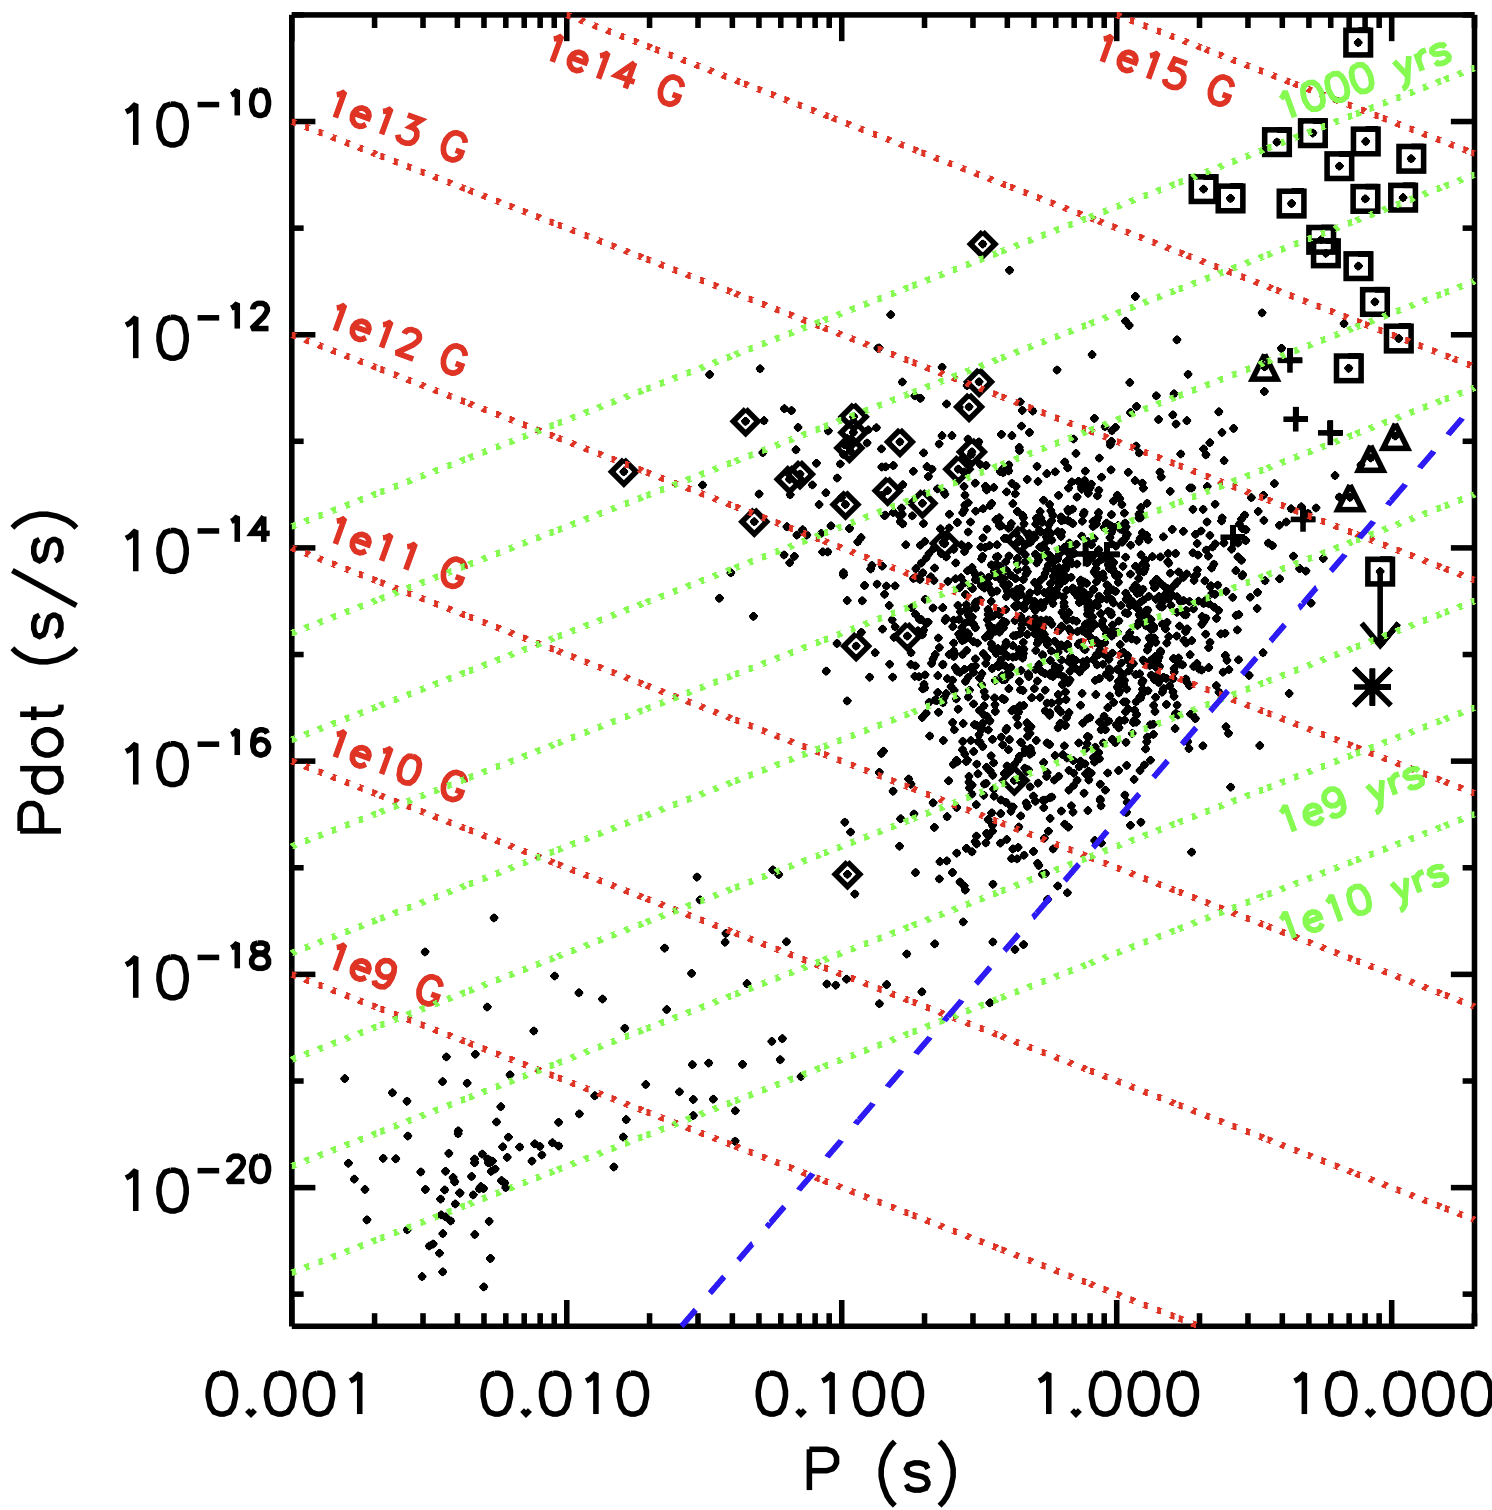
\includegraphics[width=0.7\textwidth]{Figures/Intro/PP.png}
    \caption{$P-\dot{P}$ diagram of pulsars in the ATNF catalog~\cite{2011AIPC.1357..269T,2005AJ....129.1993M}. }
    \label{fig:pp}
\end{figure}

\subsection{High-energy emission}

\subsection{Population in the Galactic bulge}



% The millisecond pulsar population remains a viable sources for the GCE. 


\section{Stellar mass distribution in the Galactic bulge}\label{se:bulge_model}

The stellar mass distribution in the inner Galaxy is unique and complicated. It shares few feature with the dark matter distribution (the NFW profile), which is spherically symmetric. The morphology of the GCE provide a viable probe for the origin of the excess.

\subsection{Boxy Bulge}

The mid- and near-IR signals of the inner Galaxy stars reveal a bar structure. The Galactic bar makes a tilt angle $\theta_0$ from the GC-Sun direction while the Sun is located at $\sim$10 pc above the Galactic plane. The line-of-sight view of the Galactic bar shows a boxy shape, so it is often referred as the Boxy Bulge. Here, we introduce the bar model derived from data taken with the Diffuse Infrared Background Experiment instrument on board the Cosmic Background Explorer~\cite{1998ApJ...492..495F}. The shape of the bar is a generalized ellipsoid which can be parametrized as
\begin{align}\label{eq:Rs}
  R_{\perp}^{C_{\perp}} &= \left(\dfrac{|X'|}{a_x}\right)^{C_{\perp}} + \left(\dfrac{|Y'|}{a_y}\right)^{C_{\perp}},\\
  R_s^{C_{\parallel}} &= R_{\perp}^{C_{\parallel}} + \left(\dfrac{|Z'|}{a_z}\right)^{C_{\parallel}},
\end{align}
where $R_s$ is the effective radius; $a_x$, $a_y$, and $a_z$ are the scale lengths; $C_\perp$ and $C_\parallel$ are the face-on and edge-on shape parameters; and $X'$, $Y'$, and $Z'$
are directions in the bar
coordinate. 
% Reference~\cite{1998ApJ...492..495F} considered three different models for the radial dependence: model S, $\rho\propto\text{sech}^2(R_s)$; model E, $\rho\propto\exp(R_s^{-n})$; model P, $\rho\propto[1+(R_s/R_c)^n]$. We use model S here since it was the best-fit model found in Ref.~\cite{1998ApJ...492..495F}.

The models are truncated by a Gaussian function at the
radius $R_{\text{end}}$ with scale length $h_{\text{end}}$. For model S in Ref~\cite{1998ApJ...492..495F}, the density of the bar~\footnote{We notice that there was a typo in the argument of the $\exp$ function in Eq.(14) of Ref~\cite{1998ApJ...492..495F} which has been corrected in our Eq.~\ref{eq:Rs}. We have confirmed this in private communication with H. Freudenreich.} is given by,
\begin{equation}\label{eq:rhobar}
  \rho_{\text{bar}}\propto \begin{cases}
    \text{sech}^2(R_s), & R \leq R_{\text{end}},\\
    \text{sech}^2(R_s)e^{-\frac{(R-R_{\text{end}})^2}{h_{\text{end}}^2}}, &   R > R_{\text{end}}.
  \end{cases}
\end{equation}

The bar parameters 
%used in our work 
are displayed in Table~\ref{tab:modelS}. These correspond to the best-fit values for model S using the so-called primary mask~\cite{1998ApJ...492..495F}. Overall, the stellar mass of the Galactic bulge is $(1.4-1.7)\times 10^{10}$ solar masses $(M_\odot)$~\cite{2016ARA&A..54..529B}.
% Recent studies of the bulge suggest larger tilt angles of $\sim 30^\circ$~\cite{2013MNRAS.434..595C,2017MNRAS.465.1621P}. However, we keep the best-fit angle from Ref.~\cite{1998ApJ...492..495F} since it is consistent with the ISRF implemented in \textsc{galprop} v54. Also, as we discuss later, we do not expect the IC emissions to be very sensitive to this angle. Overall, the stellar mass of the Galactic bulge is $(1.4-1.7)\times 10^{10}$ solar masses $(M_\odot)$~\cite{2016ARA&A..54..529B}.

% \begin{table}[htb]
% \centering
% \caption{Approximate computation times in hh:mm:ss for full order 						versus reduced order models.}
% \begin{tabular}{ccc}
% \toprule
% & \multicolumn{2}{c}{Computation Time}\\
% \cmidrule(r){2-3}
% $\overline{U}_{in}$ m/s & Full Model & ROM \\
% \midrule
% 0.90 & 2:00:00 & 2:08:00\\
% 0.88 & 2:00:00 & 0:00:03\\
% 0.92 & 2:00:00 & 0:00:03\\
% \midrule
% Total & 6:00:00 & 2:08:06\\
% \bottomrule
% \end{tabular}
% \label{tab:time_rom}
% \end{table}

\begin{table}[htb]
\centering
\caption{ The parameter values for the Galactic bar model S of Ref.~\cite{1998ApJ...492..495F}.}
    \begin{tabular}{ll}
    \toprule
      Parameters & Model S \\ 
      \midrule
      Distance to the Galactic Plane $Z_0$ (pc) & 16.46 $\pm$ 0.18\\
      Bar Tilt Angle $\theta_0$ (deg) & 13.79 $\pm$ 0.09\\
      Bar $X$ Scale Length $a_x$ (kpc) & 1.696 $\pm$ 0.007 \\
      Bar $Y$ Scale Length $a_y$ (kpc) & 0.6426 $\pm$ 0.0020 \\
      Bar $Z$ Scale Length $a_z$ (kpc) & 0.4425 $\pm$ 0.0008 \\
      Bar Cutoff Radius $R_{\text{end}}$ (kpc) & 3.128 $\pm$ 0.014 \\
      Bar Cutoff Scale Length $h_{\text{end}}$ (kpc) & 0.461 $\pm$ 0.005 \\
      Bar Face-On Shape $C_\perp$ & 1.574 $\pm$ 0.014 \\
      Bar Edge-On Shape $C_\parallel$ & 3.501 $\pm$ 0.016\\
      \bottomrule
    \end{tabular}
\label{tab:modelS}
\end{table}

\subsection{Nuclear bulge}\label{sec:nb}

The Nuclear Bulge refers to a dense stellar structure contained in the innermost region of the Galaxy. 
Reference~\cite{2002A&A...384..112L} revealed the distribution of stars and interstellar matter in the Nuclear Bulge from IRAS and COBE DIRBE data. Associated with the Central Molecular Zone of the Galaxy, the Nuclear Bulge has younger stars and undergoes active star formation, distinguishing it from the old and evolved stars of the Galactic bulge~\cite{2002A&A...384..112L}. 
% The Nuclear Bulge makes up around 10\% of the stellar mass in the bulge and its gamma-ray luminosity is comparable with that of the Galactic bulge~\cite{2018NatAs...2..387M,2018NatAs...2..819B}. 
The Nuclear Bulge resides within the inner 230 pc of the GC and is made of two components:

\paragraph{Nuclear stellar cluster (NSC):} The NSC is a relatively small and very dense spherically symmetric structure in the innermost part of the NB. The stellar density in this region has been shown~\cite{2002A&A...384..112L} to be well described by a simple radial power-law function
\begin{equation}\label{eq:NSC}
  \rho_{\text{NSC}}(R)=\dfrac{\rho_0}{1+\left(\dfrac{R}{R_0}\right)^{n}},
\end{equation}
with best-fit power-law indices $n = 2.0$ for $R \leq 6$ pc and $n = 3.0$ for $R > 6$ pc, with core radius fixed to $R_0 = 0.22$ pc. The stellar mass of the entire NSC is $(3\pm$ 1.5) $\times$ 10$^7$ $M_\odot$.

\paragraph{Nuclear stellar disk (NSD):} Surrounding the NSC is the NSD which makes up most of the stellar mass of the NB. The NSD is a cylindrical object with a radial dependence approximately described by a broken power-law function,
\begin{equation}\label{eq:NSD}
  \rho_{\text{NSD}}(r) = \begin{cases}
    \rho_0\ r^{-0.1}, & r < 120\ \text{pc},\\
    \rho_1\ r^{-3.5}, & 120\ \text{pc} \leq r < 220\ \text{pc},\\
    \rho_2\ r^{-10}, & r \geq 220\ \text{pc}.
  \end{cases}
\end{equation}
The scale densities $\rho_0$, $\rho_1$, and $\rho_2$ ensure the continuity of the NSD density function. The density variation along the $z$ direction is given by an exponential cutoff with a scale height 45 $\pm$ 5 pc. The stellar mass of the entire NSD is (1.4 $\pm$ 0.6) $\times$ 10$^9$ $M_\odot$.

\section{Morphology of the GCE}



% \subsubsection{X-shaped Bulge}

% The X-shaped bulge \citep{2016AJ....152...14N} is potentially another structure of stars in the inner Galaxy. It has been extracted from WISE W1 and W2 data at $3.4$ and $4.6\,\mrm{\mu m}$, respectively.
% %
% It is argued that the Milky Way bulge is morphologically X-shaped, following from expectations of dynamical models and observations of other barred galaxies.
% %
% Further, the population of stars leading to this shape due of their orbital motion contribute to about 40--45\% of the total bulge mass \citep{2015MNRAS.450L..66P}.
% %
% This fraction can be used to estimate the luminosity of the X-bulge template, as it is not parametrised in 3D.
% %
% The arms of the WISE X-bulge (see Fig.\,\ref{fig:XB_map}) appear asymmetric, being longer for positive longitudes ($l \lesssim 7.5^{\circ}$) than for negative longitudes ($l \gtrsim -5^{\circ}$).
% %
% This is interpreted as a projection effect of the bulge being $27^{\circ}$ tilted to the line of sight \citep{2013MNRAS.435.1874W}.
% %
% The X-bulge is thus said to trace faint red clump stars with its short arms more distant to the Sun and bright red clump with its long arms closer to the Sun \cite[][cf. discussion about the `double red clump' of the Milky Way]{2018ApJ...862L...8L}.
% %
% However, we note that the remaining WISE bands W3 and W4 at $12$ and $22\,\mrm{\mu m}$, respectively, mainly trace dust between $\approx 100$ and $250\,\mrm{K}$ rather than star light and show no enhanced X-shape.

% Figure~\ref{fig:bulge_templates} shows the maps for the Boxy Bulge (left), Nuclear Bulge (middle), and X-bulge (right).

% \begin{figure}
%     \centering
%     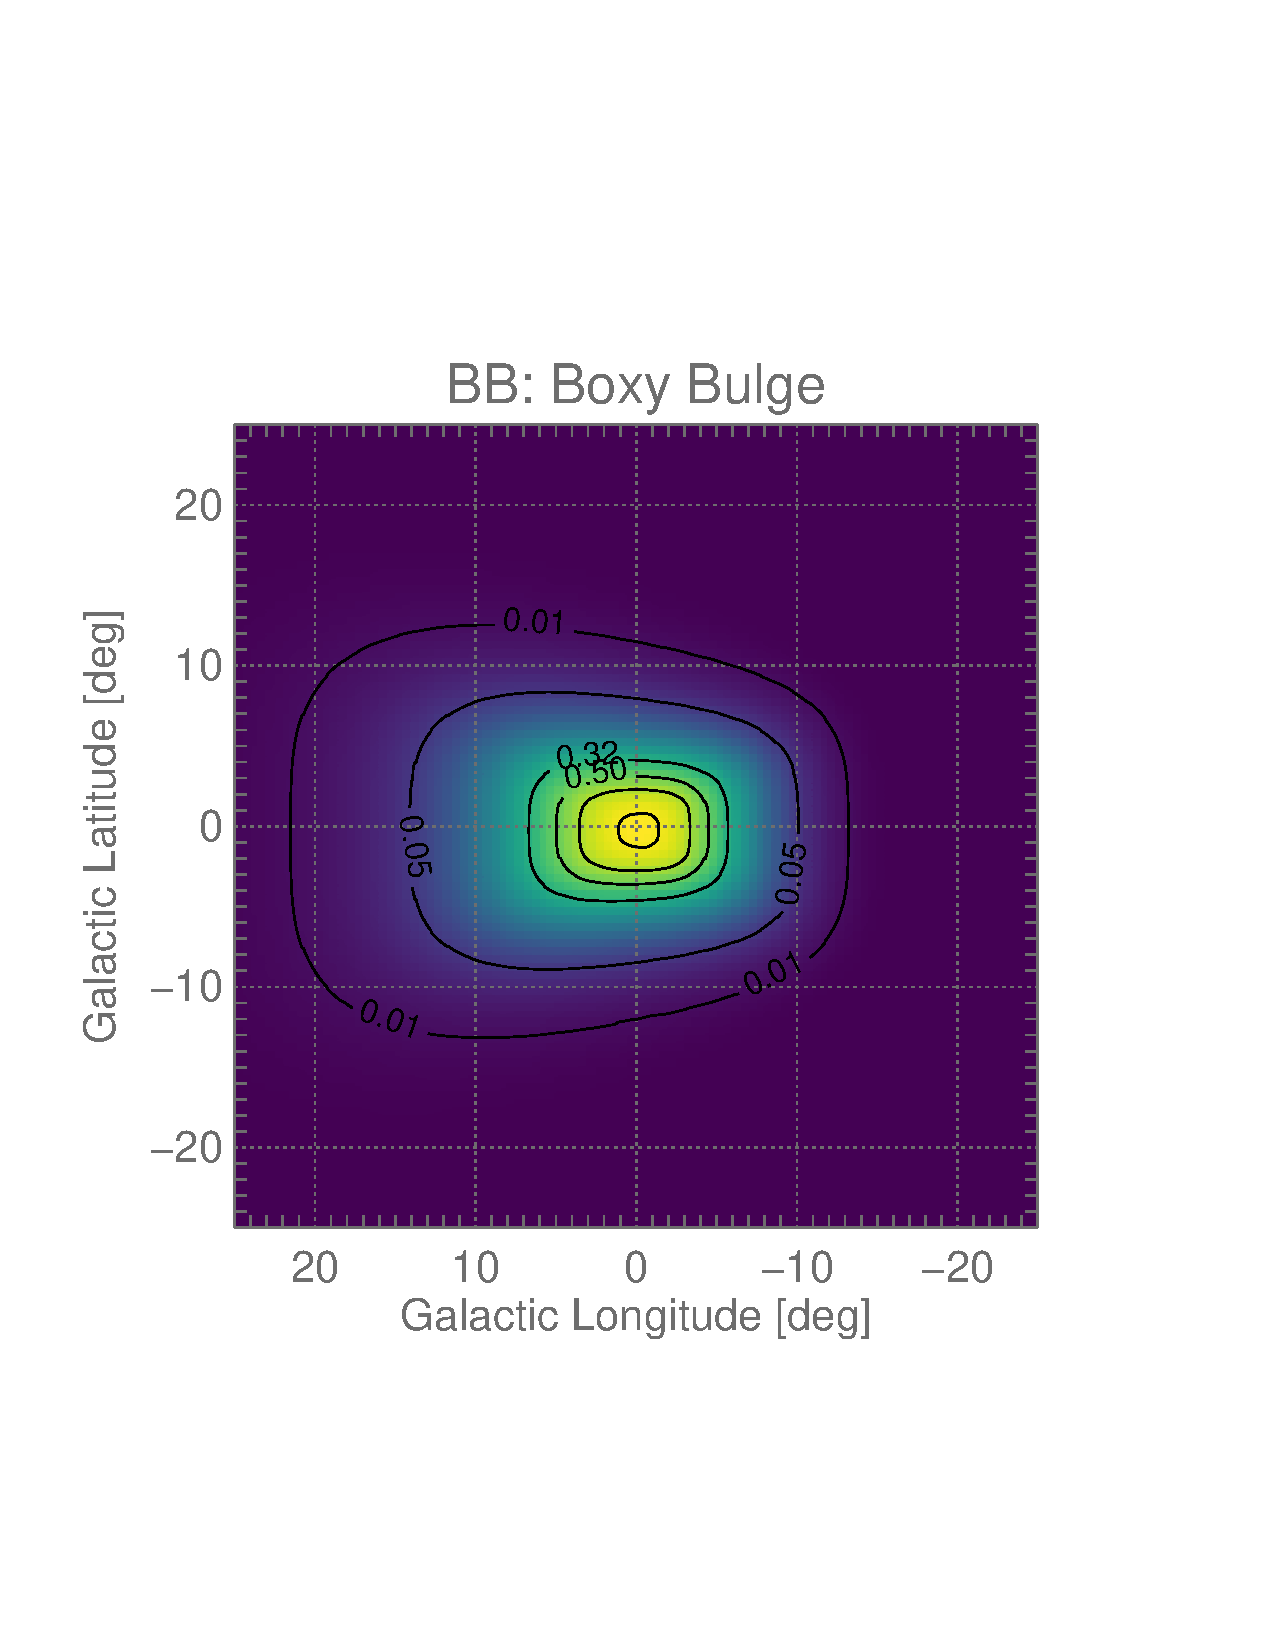
\includegraphics[width=0.32\textwidth]{Figures/511keV/map_BB_asinh_grid.pdf}
%     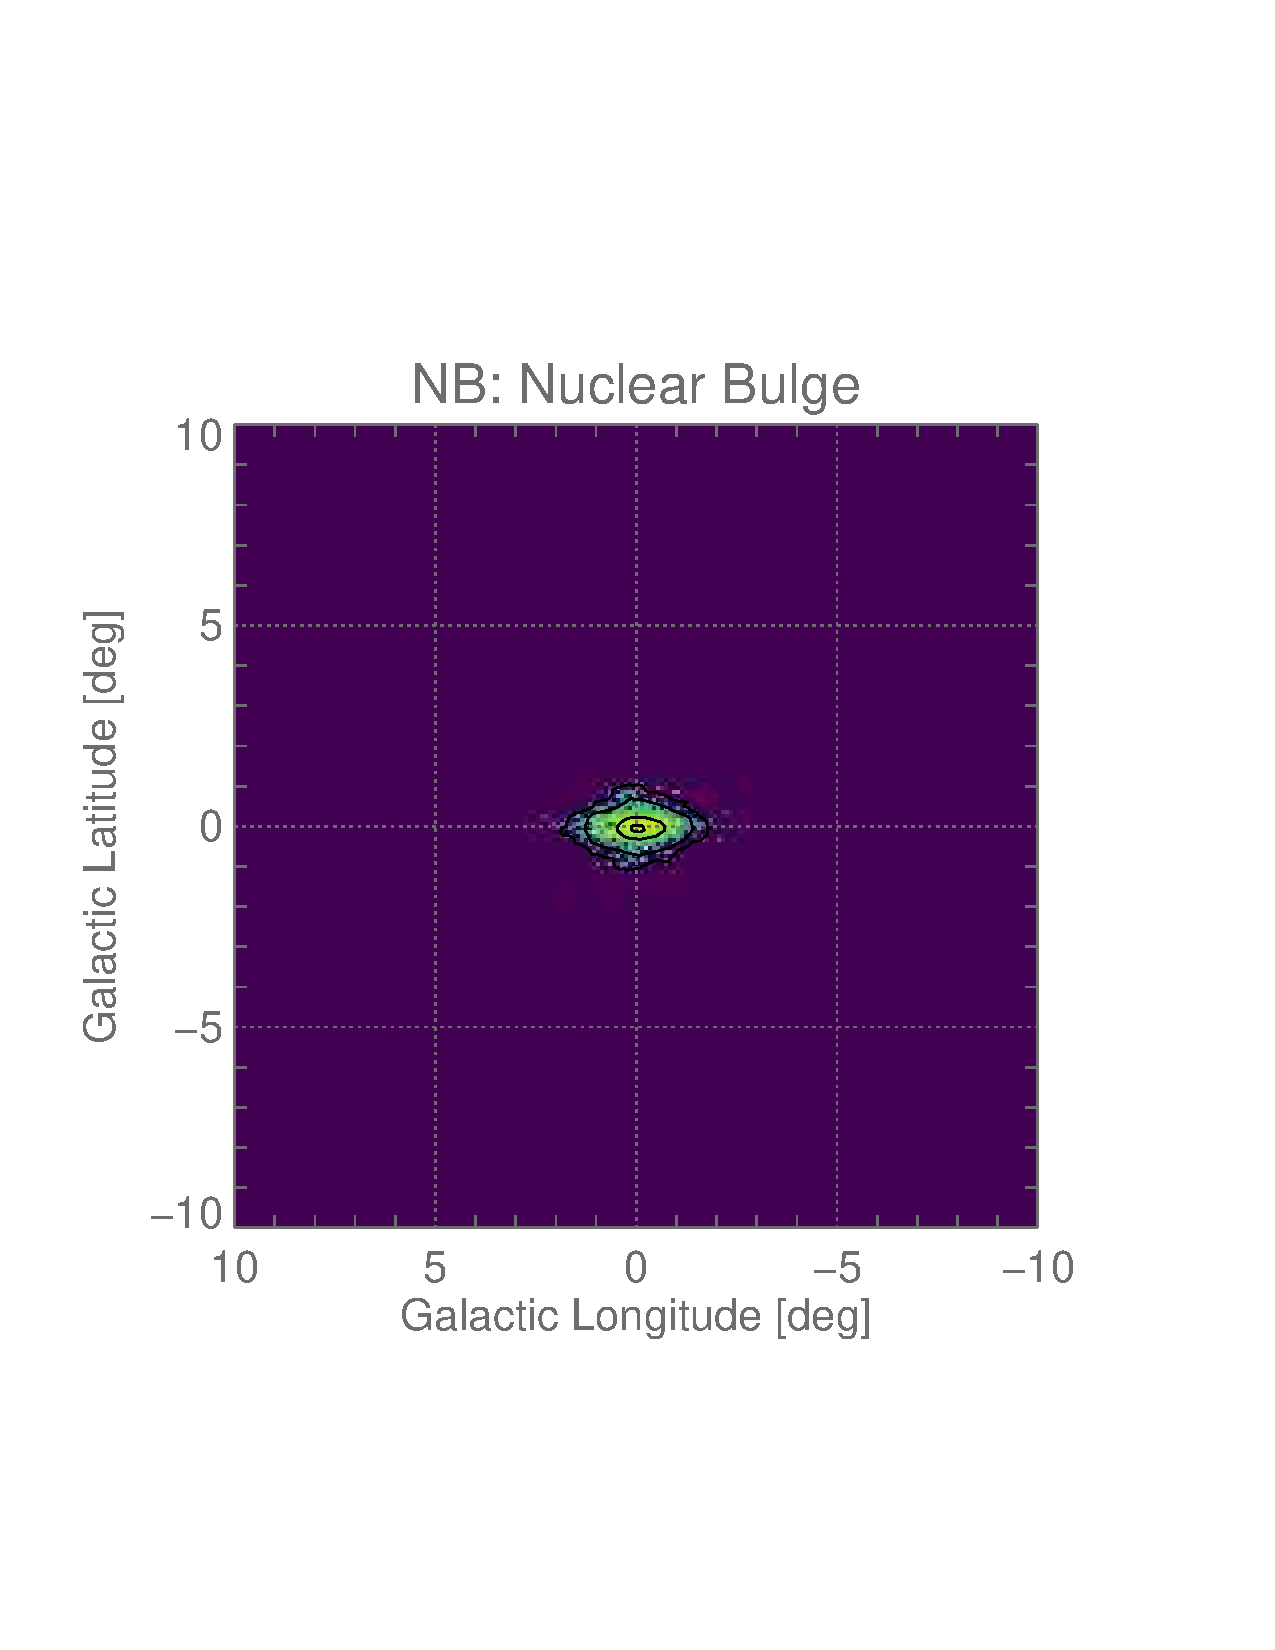
\includegraphics[width=0.32\textwidth]{Figures/511keV/map_NB_log_grid_20x20.pdf}
%     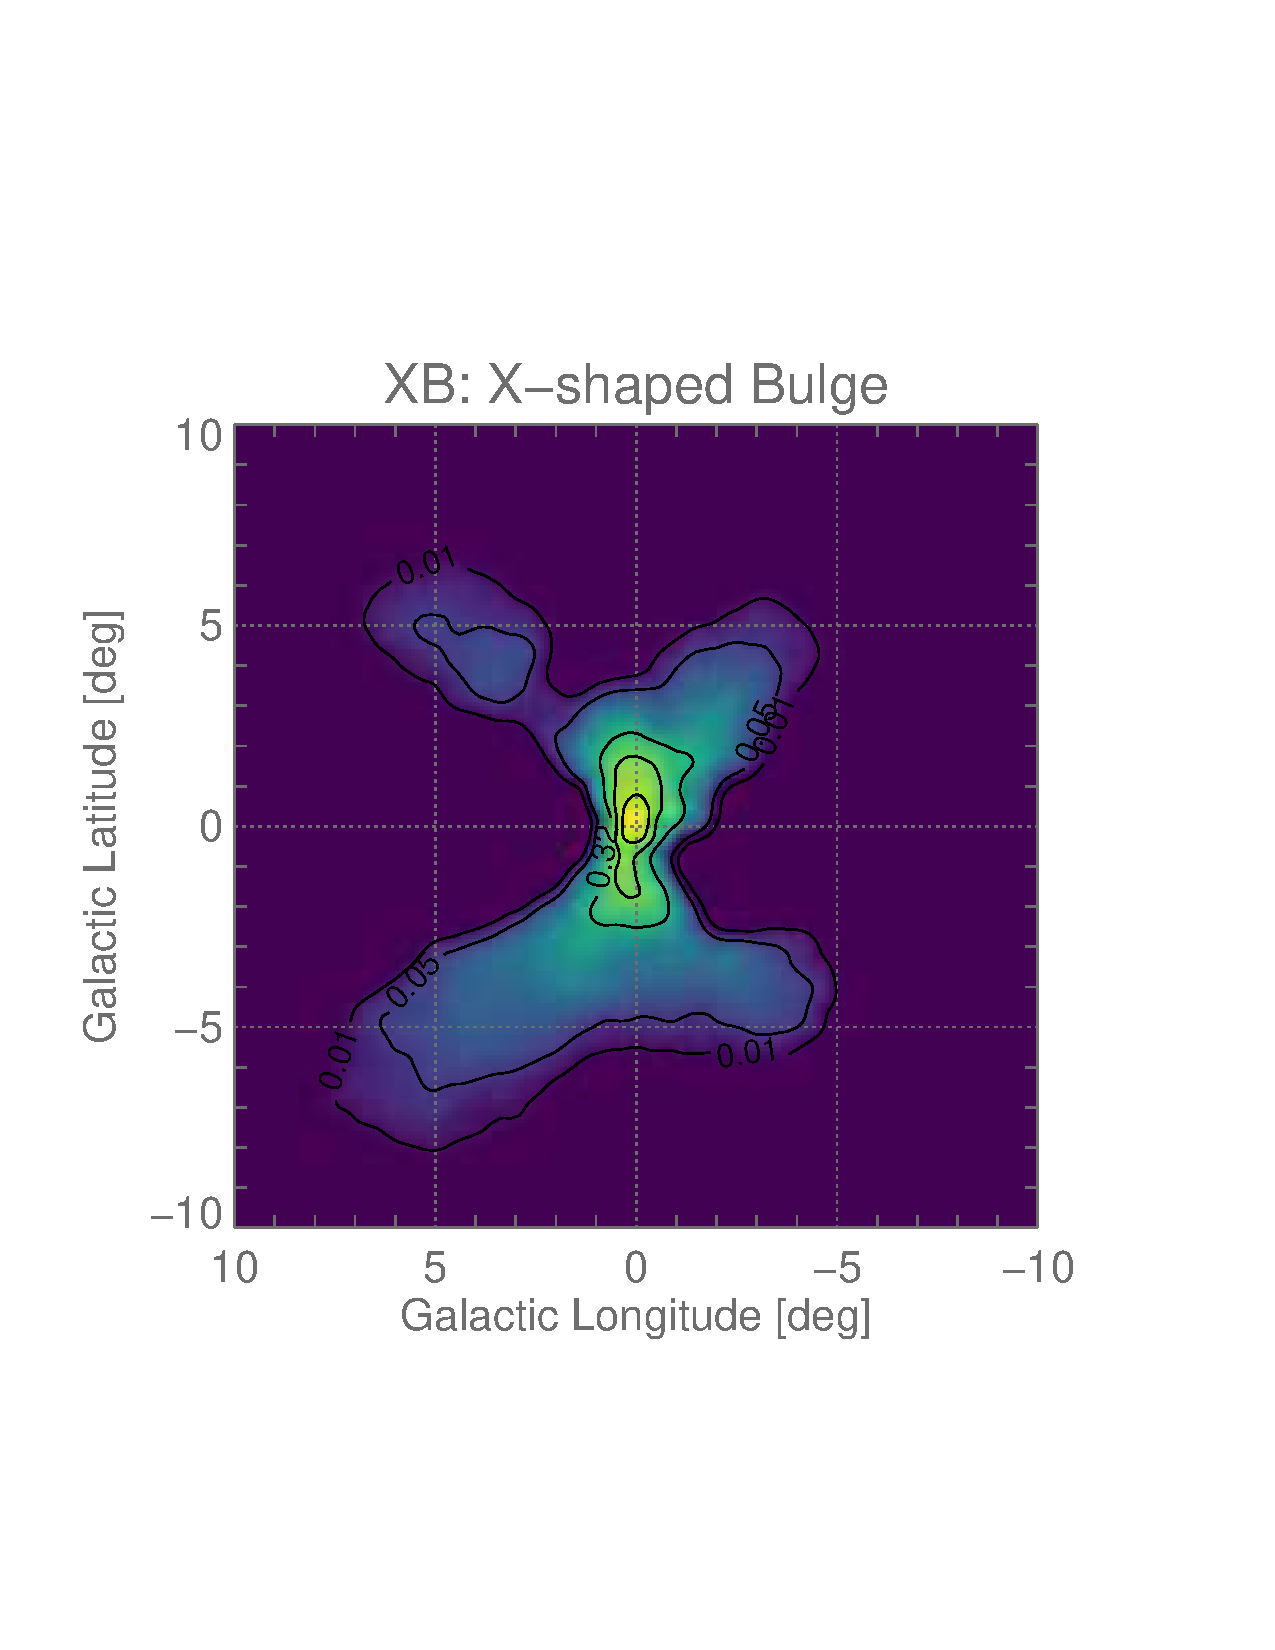
\includegraphics[width=0.32\textwidth]{Figures/511keV/map_XB_asinh_grid_20x20.pdf}
%     \caption{Maps for the Boxy Bulge (left), Nuclear Bulge (middle), and X-bulge (right). Figures are reproduced based on the best-fit models in Ref.~\cite{1998ApJ...492..495F, 2002A&A...384..112L,2016AJ....152...14N}.}
%     \label{fig:bulge_templates}
% \end{figure}


\chapter{Inverse Compton emission from millisecond pulsars in the Galactic bulge} \label{ch:IC_MSPs}

\section{Abstract}

Analyses of \textit{Fermi} Large Area Telescope data have revealed a source of excess diffuse gamma rays towards the Galactic center that extends up to roughly $\pm 20$ degrees in latitude. The leading theory postulates that this GeV excess is the aggregate emission from a large number of faint millisecond pulsars (MSPs). The electrons and positrons ($e^{\pm}$) injected by this population could produce detectable inverse-Compton (IC) emissions by up-scattering ambient photons to gamma-ray energies. In this chapter, we calculate such IC emissions using \textsc{galprop}. A triaxial 3D model of the bulge stars obtained from a fit to infrared data is used as a tracer of the putative MSP population. This model is compared against one in which the MSPs are spatially distributed as a Navarro-Frenk-White squared profile. We show that the resulting spectra for both models are indistinguishable, but that their spatial morphologies have salient recognizable features. The IC component above $\sim $ TeV energies carry information on the spatial morphology of the injected $e^\pm$. Such differences could potentially be used by future high-energy gamma-ray detectors such as Cherenkov Telescope Array (CTA) to provide a viable multiwavelength handle for the MSP origin of the GeV excess.

\section{Attribution}

This chapter is based on the following publication of which I am the first author:
\begin{itemize}
    \item \emph{Song, D., Macias, O., and Horiuchi, S., “Inverse Compton emission from millisecond pulsars in the Galactic bulge”, Physical Review D, vol. 99, no. 12, 2019}
    % \item \emph{Macias, O., van Leijen, H., Song, D., Ando, S., Horiuchi, S., and Crocker, R. M., “Cherenkov Telescope Array sensitivity to the putative millisecond pulsar population responsible for the Galactic Centre excess”, Monthly Notices of the Royal Astronomical Society, vol. 506, no. 2, 2021}
    % \item \emph{Song, D., Macias, O., Horiuchi, S., Crocker, R. M., and Nataf, D. M., “Evidence for a high-energy tail in the gamma-ray spectra of globular clusters”, Monthly Notices of the Royal Astronomical Society, vol. 507, no. 4, 2021}
    % \item \emph{Siegert T., Crocker R.~M., Macias O., Panther F.~H., Calore F., Song D., Horiuchi S, “Measuring the smearing of the Galactic 511 keV signal: positron propagation or supernova kicks?”, Monthly Notices of the Royal Astronomical Society Letters, accepted for publication, 2021}
\end{itemize}
With the help of Oscar Macias, I modified the \textsc{galprop} code to include the $e^\pm$ injection from millisecond pulsars. Using the modified code, I calculated IC emission with various injection models and made plots to illustrate the results. All authors are involved in the discussion and interpretation of the results.

\section{Introduction}

In the past decade, the \emph{Fermi} Large Area Telescope (LAT) has provided accurate observations of the gamma-ray sky, of which the Galactic center remains one of the most intriguing and intricate regions. It is of paramount importance to map the gamma-ray emissions from the Galactic center to better understand the properties of cosmic rays (CRs), the interstellar medium (ISM), and tests of dark matter (DM) in the inner regions of our Galaxy. Using template fitting techniques to regress out the Galactic and extragalactic diffuse emissions, multiple studies~\cite{2009arXiv0910.2998G,2009arXiv0912.3828V,2011PhLB..697..412H,2012PhRvD..86h3511A,2013PhRvD..88h3521G,2014PhRvD..89f3515M,2013PDU.....2..118H,2014PhRvD..90b3526A,2016PDU....12....1D,2015JCAP...03..038C,2015PhRvD..91l3010Z,2016ApJ...819...44A,2017ApJ...840...43A} have found an excess of gamma rays towards the Galactic center extending up to $\sim\pm$20 degrees in latitude. Often referred to as the Galactic center excess (GCE), this excess emission has a centrally peaked spatial morphology that is roughly spherically symmetric with a radial power law of slope $\sim$2.4, and a curved energy spectrum peaking at $\sim$3 GeV. Some authors have argued that the GCE is consistent with a DM emission~\cite{2009arXiv0910.2998G,2012PhRvD..86h3511A,2013PhRvD..88h3521G,2014PhRvD..89f3515M,2015JCAP...03..038C,2016PDU....12....1D} given its similarities to simplified predictions of weakly interacting massive particle DM models.

However, studies have also shown that the origin of the GCE can be explained by astrophysical sources, such as a population of unresolved gamma-ray-emitting millisecond pulsars (MPSs)~\cite{2011JCAP...03..010A,2012PhRvD..86h3511A,2013PhRvD..88h3521G,2014PhRvD..89f3515M,2015JCAP...03..038C,2016PDU....12....1D}. While there is ongoing debate regarding the consistency of the GCE with the luminosity function of MSPs measured elsewhere in the Galaxy\cite{2015JCAP...06..043C, 2016JCAP...03..049H, 2017JCAP...08..015P, 2018MNRAS.481.3966B}, evidence supporting the MSP hypothesis is mounting. For example, population synthesis simulations~\cite{2018ApJ...863..199G} show that $\sim 10^4$ MSPs can inhabit the Galactic center region and explain the GCE. Also, subthreshold photon-count statistics have shown detectable features that can be used to distinguish between the MSPs and DM interpretations of the GCE. In particular, Refs.~\cite{2016PhRvL.116e1103L,2017AJ....153..253M} introduced a new statistical technique called the non-Poissonian template fit which can be used for characterizing populations of unresolved point sources at fluxes below the detection threshold. They have shown that an unresolved population of point sources just below the sensitivity of the LAT is responsible for the GCE.

More recently, Refs.~\cite{2018NatAs...2..387M, 2018NatAs...2..819B,  2019JCAP...09..042M} investigated whether the spatial morphology of the GCE is better described by the distribution of stars or by DM. It has been firmly established that the bulk of the stars in the Galactic center region form a so-called box/peanut-bulge structure~\cite{1995ApJ...445..716D,1998ApJ...492..495F,2000MNRAS.313..392L,2010ApJ...721L..28N,2013MNRAS.435.1874W}. The density distribution of these bulge stars can be reasonably described by a triaxial geometric function~\cite{1998ApJ...492..495F,2010ApJ...721L..28N,2013MNRAS.435.1874W} extending in length to a few kpc from the Galactic center. In addition to the box/peanut-bulge, there is a distinct stellar population in the innermost $\sim$200 pc of the Galaxy called the nuclear bulge (NB)~\cite{2013ApJ...769L..28N}. Reference~\cite{2018NatAs...2..387M} used two different stellar maps for the box/peanut-bulge~\cite{1998ApJ...492..495F,2016AJ....152...14N} and also considered the NB of Ref.~\cite{2013ApJ...769L..28N}, and demonstrated that such nonspherical bulge morphologies provide a significantly better fit to the GCE than a spherical Navarro-Frenk-White squared (NFW$^2$) spatial map describing a DM annihilation signal. Importantly, that article showed that once a bulge model is included in the analysis, there is no longer statistically significant evidence for a NFW$^2$ component. These results have been corroborated by Ref.\cite{2018NatAs...2..819B} using a different and more flexible analysis method~\cite{2017JCAP...08..022S} and by Ref.~\cite{2019JCAP...09..042M} using an improved Galactic diffuse emission model.

The population of MSPs in the Galactic bulge would not only produce prompt gamma-ray emission correlated with their spatial distribution, but also inject $e^\pm$ into the interstellar environment. These CR $e^\pm$ can produce secondary emissions by interacting with the ISM and magnetic field. It has been pointed out that while the prompt gamma rays from MSPs are expected to follow the morphology of the source distribution, secondary emissions---inverse Compton (IC), bremsstrahlung, and synchrotron radiation---are expected to have different morphologies, since they also depend on their relevant targets, i.e., the interstellar radiation field (ISRF), the gas distribution, and the magnetic field of the Galaxy, respectively. The IC component is a result of an energy-dependent convolution of the spatial morphology of the CR $e^\pm$ sources with the ambient photon fields from starlight, infrared (IR) light, and the cosmic microwave background (CMB).

Previous works~\cite{2015ApJ...802..124Y,2015JCAP...02..023P} have studied the secondary IC emission at $\sim$GeV-TeV energies from MSP $e^\pm$ interacting with the ISRF assuming a \emph{spherically symmetric} distribution of MSPs. Under such an assumption, Ref.~\cite{2016PhRvD..93j3004L} searched for secondary gamma-ray emission from MSPs by performing template fits to the GCE data, and found it to be difficult to detect or constrain the putative secondary IC component from an unresolved population of MSPs using \textit{Fermi}-LAT data alone. However, as discussed above, there is now growing evidence for a significant departure from spherical symmetry.

Nonspherical source morphologies have been explored on small ($<$1 kpc) scales. For example, in a region overlapping with the NB called the Galactic ridge, Ref.~\cite{2015MNRAS.451.1833M} showed that several different CR scenarios can explain the multiwavelength data taken from this patch of the sky. In addition, Ref.~\cite{2016PhRvL.117k1101C} evaluated the impact of star-forming activity in the Galactic ridge on the GCE properties. The study by Ref.~\cite{2017PhRvL.119c1101G} solved the diffusion equation for CRs with a position-dependent diffusion coefficient and explained the recent H.E.S.S.~\cite{2016Natur.531..476H} measurements from this region by the interaction of the CRs with the gas in the central molecular zone (CMZ). Reference~\cite{2018JCAP...07..042G} explained the H.E.S.S. measurements by MSPs accelerating CR protons.

In this chapter, we revisit the IC emission from MSP $e^\pm$ focusing on a potential \emph{nonspherical} source morphology related to the Galactic bulge structure. Reference~\cite{2015JCAP...07..013A} looked for and found a gamma-ray component following the IR distribution in the Galactic center. The authors interpreted this as IC emission correlating with the distribution of optical light, but a propagation of the underlying $e^\pm$ was not performed. Here, we use the publicly available propagation code \textsc{galprop}\footnote{http://galprop.stanford.edu}\cite{2000ApJ...537..763S} and make detailed predictions for the spectrum and morphology of the IC emission at 100 MeV-100 TeV energies. For the spatial morphology of MSP $e^\pm$, we use a three-dimensional (3D) stellar distribution model for the Galactic bulge obtained from a fit to IR data~\cite{1998ApJ...492..495F} as well as one for the NB~\cite{2002A&A...384..112L} stars. We also show detailed comparisons against the spectrum and morphology obtained when the unresolved populations of MSPs are assumed to be spherically distributed. We find salient recognizable differences on large spatial scales and energies above $\sim$TeV, which can be used to distinguish source spatial morphologies.

This chapter is structured as follows. In Sec.~\ref{sec:spatial} we describe the 3D models used for the spatial distribution of the putative MSP population in the Galactic center. In Sec.~\ref{sec:prop} we provide details about the propagation setup and configuration of our \textsc{galprop} runs. Details about the assumed MSP injection spectra are also given in this section. Our main results are shown in Sec.~\ref{sec:results_IC}, where we show the predicted spectrum and morphology for the IC emission at $\sim$GeV-TeV energies. We illustrate how future measurements of diffuse gamma-ray emission with the Cherenkov Telescope Array (CTA)~\cite{2009arXiv0912.3742W,2011ExA....32..193A} have the potential to constrain the main properties of this purported MSP population at the Galactic center. Finally, we conclude our study in Sec.~\ref{sec:conclu}.

\section{Spatial distributions}\label{sec:spatial}

To propagate the $e^\pm$ injected by MSPs, we need to model their spectrum and the spatial distribution of MSPs. We first discuss the spatial distribution. Two scenarios are considered: the stellar mass distribution in the Galactic bulge, and the spherically symmetric model for comparison.

\subsection{Stellar models}\label{sec:stellar}

We describe our first scenario, in which an unresolved population of MSPs is created \emph{in situ} in the inner Galaxy and follows the distribution of stellar mass. Assuming that the same stellar populations responsible for the IR bulge trace the distribution of MSPs, a reasonable starting point for the MSP distribution is the bulge morphology itself. In principle, a proper morphological calculation would need to take into account the kick velocities of the MSP seeds at birth~\cite{2018ApJ...862...79E}. However, the kicks experienced by MSPs should be lower than for isolated pulsars, which is also necessary for them to be confined to globular clusters. For example, while isolated pulsars are consistent with a Maxwellian velocity distribution with dispersion of 190 km/s~\cite{1997MNRAS.291..569H}, MSP estimates fall in the ranges $10-50$~\cite{2013PhRvD..88h3009H,1997ApJ...482..971C}, $85\pm13$~\cite{2004IAUS..218..139H}, or at the high end $130\pm30$ km/s~\cite{1998MNRAS.295..743L}. Thus for our MSP estimates we do not consider the effects of initial kicks, and we consider the spatial distribution of stars using the 3D Galactic bulge model of Ref.~\cite{1998ApJ...492..495F} and the NB model of Ref.~\cite{2002A&A...384..112L}.

The details and parameters of the bulge models are the same as those summarized in Sec.~\ref{se:bulge_model}. Recent studies of the bulge suggest larger tilt angles of $\sim 30^\circ$~\cite{2013MNRAS.434..595C,2017MNRAS.465.1621P}. However, we keep the best-fit angle from Ref.~\cite{1998ApJ...492..495F} since it is consistent with the ISRF implemented in \textsc{galprop} v54. Also, as we discuss later, we do not expect the IC emissions to be very sensitive to this angle.

% \subsubsection{Galactic bulge}\label{sec:bulge}

% The mid- and near-IR signals of the inner Galaxy stars reveal a bar structure. The Galactic bar makes a tilt angle $\theta_0$ from the GC-Sun direction while the Sun is located at $\sim$10 pc above the Galactic plane. Here we adopt the bar model derived from data taken with the Diffuse Infrared Background Experiment instrument on board the Cosmic Background Explorer~\cite{1998ApJ...492..495F}. The shape of the bar is a generalized ellipsoid which can be parametrized as
% \begin{align}\label{eq:Rs}
%   R_{\perp}^{C_{\perp}} &= \left(\dfrac{|X'|}{a_x}\right)^{C_{\perp}} + \left(\dfrac{|Y'|}{a_y}\right)^{C_{\perp}},\\
%   R_s^{C_{\parallel}} &= R_{\perp}^{C_{\parallel}} + \left(\dfrac{|Z'|}{a_z}\right)^{C_{\parallel}},
% \end{align}
% where $R_s$ is the effective radius; $a_x$, $a_y$, and $a_z$ are the scale lengths; $C_\perp$ and $C_\parallel$ are the face-on and edge-on shape parameters; and $X'$, $Y'$, and $Z'$
% are directions in the bar
% coordinate. Reference~\cite{1998ApJ...492..495F} considered three different models for the radial dependence: model S, $\rho\propto\text{sech}^2(R_s)$; model E, $\rho\propto\exp(R_s^{-n})$; model P, $\rho\propto[1+(R_s/R_c)^n]$. We use model S here since it was the best-fit model found in Ref.~\cite{1998ApJ...492..495F}.

% The models are truncated by a Gaussian function at the
% radius $R_{\text{end}}$ with scale length $h_{\text{end}}$. For model S, the density of the bar~\footnote{We notice that there was a typo in the argument of the $\exp$ function in Eq.(14) of \cite{1998ApJ...492..495F} which has been corrected in our Eq.~\ref{eq:Rs}. We have confirmed this in private communication with H. Freudenreich.} is given by,
% \begin{equation}\label{eq:rhobar}
%   \rho_{\text{bar}}\propto \begin{cases}
%     \text{sech}^2(R_s), & R \leq R_{\text{end}},\\
%     \text{sech}^2(R_s)e^{-\frac{(R-R_{\text{end}})^2}{h_{\text{end}}^2}}, &   R > R_{\text{end}}.
%   \end{cases}
% \end{equation}

% The bar parameters used in our work are displayed in Table~\ref{tab:modelS}. These correspond to the best-fit values for model S using the so-called primary mask~\cite{1998ApJ...492..495F}. Recent studies of the bulge suggest larger tilt angles of $\sim 30^\circ$~\cite{2013MNRAS.434..595C,2017MNRAS.465.1621P}. However, we keep the best-fit angle from Ref.~\cite{1998ApJ...492..495F} since it is consistent with the ISRF implemented in \textsc{galprop} v54. Also, as we discuss later, we do not expect the IC emissions to be very sensitive to this angle. Overall, the stellar mass of the Galactic bulge is $(1.4-1.7)\times 10^{10}$ solar masses $(M_\odot)$~\cite{2016ARA&A..54..529B}.

% % \begin{table}[htb]
% % \centering
% % \caption{Approximate computation times in hh:mm:ss for full order 						versus reduced order models.}
% % \begin{tabular}{ccc}
% % \toprule
% % & \multicolumn{2}{c}{Computation Time}\\
% % \cmidrule(r){2-3}
% % $\overline{U}_{in}$ m/s & Full Model & ROM \\
% % \midrule
% % 0.90 & 2:00:00 & 2:08:00\\
% % 0.88 & 2:00:00 & 0:00:03\\
% % 0.92 & 2:00:00 & 0:00:03\\
% % \midrule
% % Total & 6:00:00 & 2:08:06\\
% % \bottomrule
% % \end{tabular}
% % \label{tab:time_rom}
% % \end{table}

% \begin{table}[htb]
% \centering
% \caption{ The parameter values for the Galactic bar model S of Ref.~\cite{1998ApJ...492..495F}.}
%     \begin{tabular}{ll}
%     \toprule
%       Parameters & Model S \\ 
%       \midrule
%       Distance to the Galactic Plane $Z_0$ (pc) & 16.46 $\pm$ 0.18\\
%       Bar Tilt Angle $\theta_0$ (deg) & 13.79 $\pm$ 0.09\\
%       Bar $X$ Scale Length $a_x$ (kpc) & 1.696 $\pm$ 0.007 \\
%       Bar $Y$ Scale Length $a_y$ (kpc) & 0.6426 $\pm$ 0.0020 \\
%       Bar $Z$ Scale Length $a_z$ (kpc) & 0.4425 $\pm$ 0.0008 \\
%       Bar Cutoff Radius $R_{\text{end}}$ (kpc) & 3.128 $\pm$ 0.014 \\
%       Bar Cutoff Scale Length $h_{\text{end}}$ (kpc) & 0.461 $\pm$ 0.005 \\
%       Bar Face-On Shape $C_\perp$ & 1.574 $\pm$ 0.014 \\
%       Bar Edge-On Shape $C_\parallel$ & 3.501 $\pm$ 0.016\\
%       \bottomrule
%     \end{tabular}
% \label{tab:modelS}
% \end{table}

% \subsubsection{Nuclear bulge}\label{sec:nb}

% The NB refers to a dense stellar structure contained in the innermost region of the Galaxy. Associated with the CMZ, the NB has younger stars and undergoes active star formation, distinguishing it from the old and evolved stars of the Galactic bulge~\cite{2002A&A...384..112L}. The NB makes up around 10\% of the stellar mass in the bulge and its gamma-ray luminosity is comparable with that of the Galactic bulge~\cite{2018NatAs...2..387M,2018NatAs...2..819B}. The NB resides within the inner 230 pc of the GC and is made of two components:

% \paragraph{Nuclear stellar cluster (NSC):} The NSC is a relatively small and very dense spherically symmetric structure in the innermost part of the NB. The stellar density in this region has been shown~\cite{2002A&A...384..112L} to be well described by a simple radial power-law function
% \begin{equation}\label{eq:NSC}
%   \rho_{\text{NSC}}(R)=\dfrac{\rho_0}{1+\left(\dfrac{R}{R_0}\right)^{n}},
% \end{equation}
% with best-fit power-law indices $n = 2.0$ for $R \leq 6$ pc and $n = 3.0$ for $R > 6$ pc, with core radius fixed to $R_0 = 0.22$ pc. The stellar mass of the entire NSC is $(3\pm$ 1.5) $\times$ 10$^7$ $M_\odot$.

% \paragraph{Nuclear stellar disk (NSD):} Surrounding the NSC is the NSD which makes up most of the stellar mass of the NB. The NSD is a cylindrical object with a radial dependence approximately described by a broken power-law function,
% \begin{equation}\label{eq:rhonsd}
%   \rho_{\text{NSD}}(r) = \begin{cases}
%     \rho_0\ r^{-0.1}, & r < 120\ \text{pc},\\
%     \rho_1\ r^{-3.5}, & 120\ \text{pc} \leq r < 220\ \text{pc},\\
%     \rho_2\ r^{-10}, & r \geq 220\ \text{pc}.
%   \end{cases}
% \end{equation}
% The scale densities $\rho_0$, $\rho_1$, and $\rho_2$ ensure the continuity of the NSD density function. The density variation along the $z$ direction is given by an exponential cutoff with a scale height 45 $\pm$ 5 pc. The stellar mass of the entire NSD is (1.4 $\pm$ 0.6) $\times$ 10$^9$ $M_\odot$.

\subsection{Spherically symmetric source}\label{sec:NFW}

Although recent reanalyses of the GCE~\cite{2018NatAs...2..387M,2018NatAs...2..819B} have shown that the \textit{Fermi}-LAT data from the inner Galaxy prefer stellar maps to spherically symmetric ones, here for comparison purposes, we also model the putative MSP population at the Galactic center with the square of an NFW density profile, of the form
\begin{eqnarray}\label{eq:NFW_2}
  \rho(R)_{\text{NFW}} = \dfrac{\rho_0}{\left(\dfrac{R}{R_\odot}\right)^\gamma\left(\dfrac{1+R/R_s}{1+R_\odot/R_s}\right)^{(3-\gamma)}},
\end{eqnarray}
where we use a core radius $R_s$ = 23.1 kpc, a Sun-GC distance $R_\odot$ = 8.25 kpc, and an inner slope of $\gamma$ = 1.20~\cite{2012PhRvD..86h3511A,2014PhRvD..89f3515M}. We label this as NFW$^2$.

\section{Propagation}\label{sec:prop}

\subsection{GALPROP code}\label{sec:galprop}

We used the publicly available software package \textsc{galprop} v54 in order to calculate the secondary gamma-ray emission from CR $e^\pm$ injected by MSPs. GALPROP is a numerical tool that solves the particle transport equations for a given source distribution and boundary conditions for all species of CRs. In particular, CRs can get accelerated by a multitude of different sources and then propagate long distances in the Galaxy. During propagation they produce secondary particles via interactions with the ISM and ISRF. Galactic diffuse gamma-ray emission is produced via $\pi_0$ decay, bremsstrahlung, and IC scattering, while lower-energy emission is produced via synchrotron radiation.

The CR $e^\pm$ transport equation is a partial differential equation of the form
\begin{align}
  \label{eq:prop_eq}
  \dfrac{d\psi}{dt} = &q(\vec{r},p)+\vec{\nabla}\cdot(D_{xx}\vec{\nabla}\psi-\vec{V}\psi)\nonumber\\
                       &+\dfrac{\partial}{\partial p}p^2D_{pp}\dfrac{\partial}{\partial p}\dfrac{1}{p^2}\psi-\dfrac{\partial}{\partial p}[\dot{p}\psi-\dfrac{p}{3}(\vec{\nabla}\cdot\vec{V})\psi],
\end{align}
where $\psi = \psi(\vec{r},p,t)$ is the density per unit of the total particle momentum, $D_{xx} = \beta D_0 (\frac{\rho}{\rho_0})^\delta$ is the spatial diffusion coefficient where $\rho$ is the rigidity of the $e^\pm$ and $\beta = v/c$, $\vec{V}$ is the convection velocity and $q(\vec{r},r)$ is the source term. Reacceleration is introduced as diffusion in momentum space with coefficient $D_{pp}$, which is related to $D_{xx}$ and the Alfv\'{e}n speed $v_A$. We refer interested readers to the excellent review in Ref.~\cite{2007ARNPS..57..285S} for more details. We keep convection off, $\vec{V}=0$.

Given the source function of MSPs, the IC energy losses at each spatial bin are calculated by
\begin{equation}
  \dot{p} = \int d(\log{\nu})\dfrac{\nu U_\nu}{\hbar \nu}\dfrac{dp}{dt}(\nu,\gamma),
\end{equation}
where $\nu$ and $U_\nu$ are the frequency and energy density of the ISRF, and $\gamma$ is the $e^\pm$ Lorentz factor. Very high-energy photons can interact with the photon fields and pair produce additional $e^\pm$ ($\gamma\gamma \to e^+e^-$). This is not included in \textsc{galprop} v54; however it only becomes important at $\sim$100 TeV, where the survival probability from the Galactic center to Earth reaches a minimum of 75-80\%~\cite{2006ApJ...640L.155M}. At 10 TeV, the effect is reduced to the percent level.

GALPROP v54 contains dedicated routines to compute the propagation of DM annihilation/decay products and predict sky maps of secondary emissions. We modify the \texttt{gen\_DM\_source.cc} routine, which allows for user-defined source functions of the DM yields (DM profile and particle spectra), to model  $e^\pm$ injected from MSPs. To compute the IC sky maps, we turn off the propagation of non-MSP CRs. As a first step, we made detailed comparisons of the results obtained with our modified GALPROP package against the literature~\cite{2014JCAP...12..045C,2016JCAP...07..041C,2015ApJ...802..124Y,2015JCAP...02..023P}. We confirm that we are able to reproduce the gamma-ray spectrum and spatial profiles of Ref.~\cite{2014JCAP...12..045C} as well as the synchrotron sky maps given in Ref.~\cite{2016JCAP...07..041C} in the context of DM annihilations. Of greater relevance to this study are our detailed checks of the results in Refs.~\cite{2015ApJ...802..124Y, 2015JCAP...02..023P}. Although we were able to reproduce the gamma-ray spectral and spatial profiles in Ref.~\cite{2015JCAP...02..023P}, we were only able to obtain the spectra given by Ref.~\cite{2015ApJ...802..124Y}. There are differences between our predicted spatial maps and those given in Fig.~3 of Ref.~\cite{2015ApJ...802..124Y} for the same propagation setup. However, we believe these differences could be due to their using older two-dimensional (2D) ISRF maps in GALPROP.

\subsection{Source function of MSP \texorpdfstring{$e^\pm$}{electrons/positrons}}\label{sec:source}

The spin-down energy $\dot E$ of MSPs is responsible for generating relativistic $e^\pm$ winds. The accelerations of these $e^\pm$ are limited when they lose energy via curvature radiation in the pulsar magnetosphere. Gamma rays are generated in this process. The gamma-ray efficiency $L_\gamma/\dot E$ is estimated to be about 10\% on average \cite{2013ApJS..208...17A}. The $e^\pm$ that escape the magnetosphere via open field lines carry a fraction $f_{e^\pm}$ of the spin-down energy into the interstellar environment. The $e^\pm$ injection luminosity of MSPs is therefore related to the gamma-ray luminosity by
\begin{equation}\label{eq:Le}
  L_{e^\pm}=f_{e^\pm}\dot{E}=10f_{e^\pm}L_\gamma.
\end{equation}
The High-Altitude Water Cherenkov Experiment (HAWC) observations of Geminga and PSR B0656+14 in the TeV energy range suggest $f_{e^\pm}$ values of $\sim$7.2-29\%~\cite{2017PhRvD..96j3013H}. Constraints by the H.E.S.S.~observations also indicate $f_{e^\pm}$ of the order 10\% if about a thousand MSPs reside in the nuclear stellar cluster around Sgr A$^*$~\cite{2013MNRAS.435L..14B}.

We normalize the two spatial templates we implement in \textsc{galprop} (stellar and NFW$^2$) by Eq.~(\ref{eq:Le}), using the best-fit gamma-ray luminosities obtained in Ref.~\cite{2018NatAs...2..387M}. The gamma-ray luminosities for the stellar template (which is a linear combination of the Galactic bar and NB models; see Sec.~\ref{sec:stellar}) are $L^{\text{bar}}_\gamma$ = (1.4 $\pm$ 0.2) $\times$ 10$^{37}$ and $L^{\text{NB}}_\gamma$ = (4.0 $\pm$ 1.0) $\times$ 10$^{36}$ erg s$^{-1}$ for the bar and NB, respectively, while the NFW$^2$ template (see~\ref{sec:NFW}) has $L^{\text{NFW}^2}_\gamma$ = (1.7 $\pm$ 0.2) $\times$ 10$^{37}$ erg s$^{-1}$. These luminosities were taken from an analysis region of size 15$^\circ$ $\times$ 15$^\circ$ around the Galactic center~\cite{2018NatAs...2..387M}.

The source term $q(\vec{r},E)$ (in units of  MeV$^{-1}$ cm$^{-2}$ s$^{-2}$ sr$^{-1}$) that is included in \textsc{galprop} can be written as the product of the injection spectrum $dN/dEdt$ and the source density distribution $\rho(\vec{r})$,
\begin{equation}
  q(\vec{r},E) = \frac{c}{4\pi} N_0 \dfrac{dN}{dEdt}\rho(\vec{r}).
\end{equation}
The factor $c/4\pi$ is a convention in the {\tt GALPROP} code. The source function is normalized by $N_0$, such that the integration over energy and volume matches Eq.~(\ref{eq:Le}),
\begin{equation}
  \label{eq:normal}
  N_0 \int E\dfrac{dN}{dEdt}dE \int\rho(\vec{r})dr^3 = L_{e^\pm} = 10 f_{e^\pm} L_\gamma.
\end{equation}
We will explore a range of $e^\pm$ spectra as detailed in Sec.~\ref{sec:spectrum}.

\begin{figure}[htb]
	\centering
	\begin{subfigure}[h]{0.45\textwidth}
		\centering
		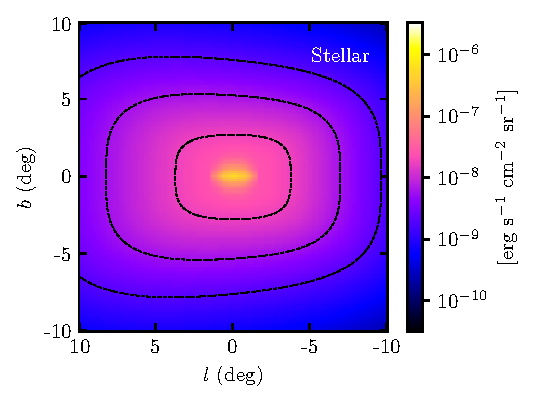
\includegraphics[width=\textwidth]{Figures/IC_MSPs/injection_skymap_bulge.pdf}
		\caption{Stellar template}
		\label{fig:injection_skymap_bulge}
	\end{subfigure}
	\begin{subfigure}[h]{0.45\textwidth}
		\centering
		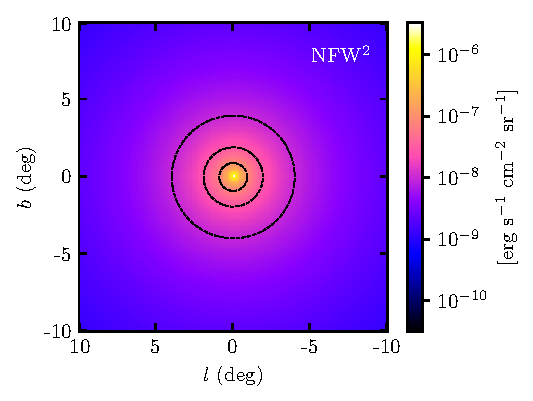
\includegraphics[width=\textwidth]{Figures/IC_MSPs/injection_skymap_nfw.pdf}
		\caption{NFW$^2$ template}
		\label{fig:njection_skymap_nfw}
	\end{subfigure}
	\caption{MSP $e^\pm$ source distributions for the stellar (a) and the NFW$^2$ (b) template over a $20^\circ \times 20^\circ$ region around the Galactic center. The normalizations are determined by gamma-ray luminosities through Eq.~(\ref{eq:Le}) (see text). The source distributions are noticeably different. While the stellar template is rectangular and asymmetric due to the tilting angle between the Galactic bar's long axis and the GC-Sun direction, the NFW$^2$ template is spherically symmetric. The very bright quasielliptical region in the central few degrees in the top panel corresponds to the NB stellar component.}
	\label{fig:injection_skymap}
\end{figure}

\begin{figure}[htb]
	\centering
	\begin{subfigure}[h]{0.45\textwidth}
		\centering
		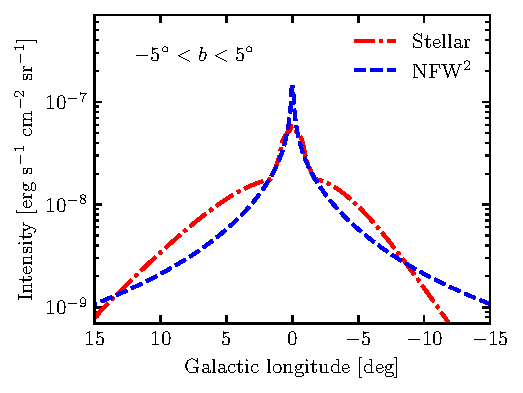
\includegraphics[width=\textwidth]{Figures/IC_MSPs/injection_lon.pdf}
		\caption{Longitudinal profiles}
		\label{fig:injection_lon}
	\end{subfigure}
	\begin{subfigure}[h]{0.45\textwidth}
		\centering
		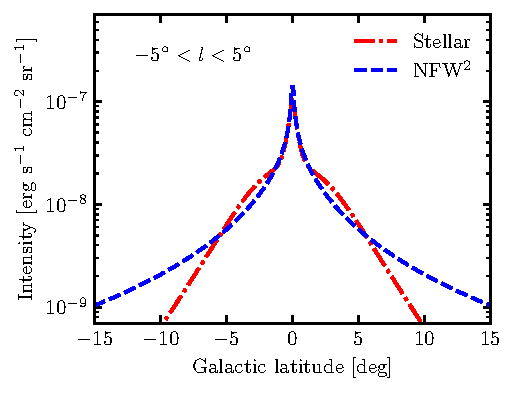
\includegraphics[width=\textwidth]{Figures/IC_MSPs/injection_lat.pdf}
		\caption{Latitudinal profiles}
		\label{fig:injection_lat}
	\end{subfigure}
	\caption{Longitudinal and latitudinal profiles for the MSP $e^\pm$ source distributions considered in this chapter. The profiles are for 10$^\circ$ wide bands and show the longitude and latitude from $15^\circ$ to $-15^\circ$. Noticeable morphological differences are seen in both directions.}
	\label{fig:injection_profile}
\end{figure}
% \begin{figure}[htb]
% \centering
%   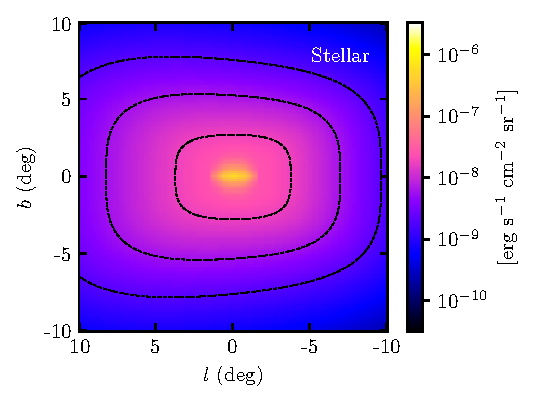
\includegraphics[width = 0.45\textwidth]{Figures/IC_MSPs/injection_skymap_bulge.pdf}
%   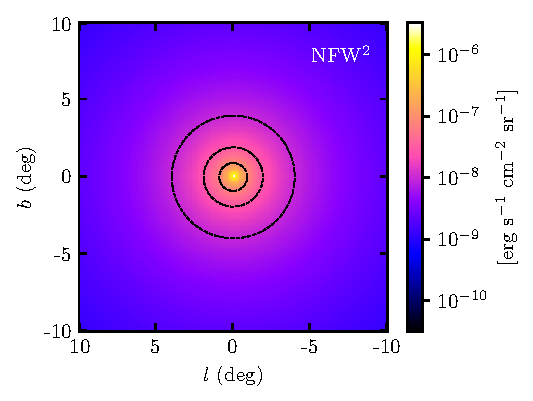
\includegraphics[width = 0.45\textwidth]{Figures/IC_MSPs/injection_skymap_nfw.pdf}
%   \caption{MSP $e^\pm$ source distributions for the stellar (top panel) and the NFW$^2$ (bottom panel) template over a $20^\circ \times 20^\circ$ region around the Galactic center. The normalizations are determined by gamma-ray luminosities through Eq.~(\ref{eq:Le}) (see text). The source distributions are noticeably different. While the stellar template is rectangular and asymmetric due to the tilting angle between the Galactic bar's long axis and the GC-Sun direction, the NFW$^2$ template is spherically symmetric. The very bright quasielliptical region in the central few degrees in the top panel corresponds to the NB stellar component.}
%   \label{fig:injection_skymap}
% \end{figure}
% \begin{figure}[t!]
%   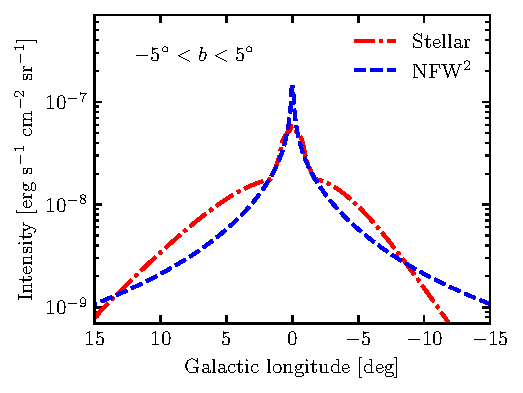
\includegraphics[width = \columnwidth]{Figures/IC_MSPs/injection_lon.pdf}
%   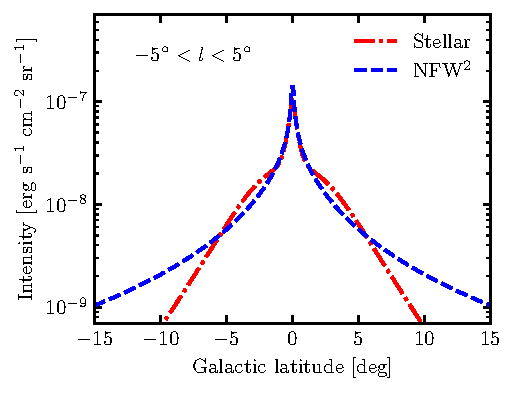
\includegraphics[width = \columnwidth]{Figures/IC_MSPs/injection_lat.pdf}
%   \caption{Longitudinal (top panel) and latitudinal (bottom panel)
%     profiles for the MSP $e^\pm$ source distributions considered in this work. The profiles
%     are for 10$^\circ$ wide bands and show the longitude and latitude
%     from $15^\circ$ to $-15^\circ$. Noticeable morphological differences are seen in both directions.}
%   \label{fig:injection_profile}
% \end{figure}

To show the source distribution and their relative injection intensities we produce injection intensity maps obtained by integrating along the line-of-sight direction the corresponding source density models,
\begin{equation}
  \label{eq:j_factor}
  I(l,b) \propto \int_{\text{l.o.s}} \rho(s,l,b) ds,
\end{equation}
where $l$ and $b$ are the galactic longitude and latitude and $s$ is the distance from the Sun along the line-of-sight direction.
Figure~\ref{fig:injection_skymap} (top panel) displays the injection intensities of the $\mbox{Galactic bar}+\mbox{NB}$ template in a 20$^\circ$ $\times$ 20$^\circ$ region around the Galactic center. The resulting sky map is oblate and asymmetric. It is brighter for positive longitudes since the long axis of the bar makes a tilting angle with the GC-Sun direction. In contrast, Fig.~\ref{fig:injection_skymap} (bottom panel) shows that the NFW$^2$ source is spherically symmetric and has a strong peak in the center of the Galaxy. We also present corresponding longitudinal and latitudinal profiles for the two models in Fig.~\ref{fig:injection_profile}. The aforementioned longitudinal asymmetry in the stellar distribution can clearly be seen in the top panel. Here it is also noticeable that the NFW$^2$ intensity profile is more strongly peaked than the stellar template. The oblateness of the $\mbox{Galactic bar}+\mbox{NB}$ model is made manifest by comparing the tails of the profiles in both panels.

\subsection{Injection spectrum}\label{sec:spectrum}

The maximum energy that MSPs can accelerate $e^{\pm}$ to is estimated to be $\sim 100$ TeV. In this work we adopt a similar $e^\pm$ spectrum to that used in Ref.~\cite{2015ApJ...802..124Y} and explore a range of parameter values. Namely, we use a power law with an exponential cutoff,
\begin{equation}
  \label{eq:msp_spectrum}
  \dfrac{dN}{dEdt} \propto E^{-\Gamma}\exp(-E/E_{\text{cut}}),
\end{equation}
where $\Gamma$ is the spectral slope and $E_{\text{cut}}$ is the energy cutoff. We vary $\Gamma$ between 1.5 and 2.5, while $E_{\text{cut}}$ is varied between 10 and 100 TeV. The combinations of spectral parameters assumed in this work are listed in Table~\ref{tab:msp_spectrum}. Note that our choice of spectral parameters represents the entire MSP population in the Galactic bulge.
\begin{table}[htb]
  \centering
  \caption{Injection spectral parameters of MSP $e^{\pm}$ adopted in this work. See Eq.~(\ref{eq:msp_spectrum}).}
    \begin{tabular}{lcc}
    \toprule
    Model Name&$\Gamma$ & $E_{\text{cut}}$\\
    & &  (TeV) \\
    \midrule
    Baseline &2.0 & 50 \\
    Inj1&1.5 & 50 \\
    Inj2&2.5 & 50 \\
    Inj3&2.0 & 10 \\
    Inj4&2.0 & 100\\
    \bottomrule
    \end{tabular}
  \label{tab:msp_spectrum}
\end{table}

\subsection{Configurations}

In order to make simulations of CR propagation that are as realistic as possible, it is crucial to understand the diffusion parameters for all the CR species. Reference~\cite{2016ApJ...824...16J} performed a scan of the parameter space of the CR injection and propagation. The scan was done separately for the low-mass isotopes ($p$, $\bar{p}$ and He) and the light elements (Be, B, C, N, O). Since each set of species has a different lifetime they probe different regions of the Galaxy. They found that the best-fit parameter setup for the low mass isotopes is different from that obtained for the heavier elements. Here, we adopt the propagation parameters for the low-mass isotopes of Ref.~\cite{2016ApJ...824...16J}. We account for uncertainties in the propagation parameters by also including the 95\% credible contours provided in their 2D marginalized posterior distributions. The propagation setups used in this work are listed in Table~\ref{tab:dpara}.

We perform 3D \textsc{galprop} simulations using the standard ISRF data available with version 54 of the software package. The calculations are made for a Cartesian spatial grid with the Galactic plane placed in the $X$-$Y$ plane and the Galactic center located at the origin of the coordinate system. The $X$ axis is defined by the GC-Sun direction.

In our simulations, the propagation volume extends to $\pm$20 kpc in both the $X$ and $Y$ direction. However, the CR halo height $z_h$ is set to different values depending on the model considered, as shown in Table~\ref{tab:dpara}. To trace the physics of the NB, we performed resolution tests for the spatial grid sizes. We fixed $\Delta Z$ = 0.125 kpc and found that the IC spectra and sky maps showed little difference when the resolution was $\Delta X$ = $\Delta Y$ = 0.125 or 0.25 kpc. We therefore adopted $\Delta X$ = $\Delta Y$ = $\Delta Z$ = 0.125 kpc for all our runs except for the $z_h = 19.28$ kpc run, which was performed at a lower resolution of $\Delta X$ = $\Delta Y$ = 0.25 and $\Delta Z$ = 0.125 kpc due to computing memory demands. As a result, each run takes about 80 hours to finish using a computer cluster node with 500 GB memory and running at $\sim 6 \times 10^{11}$ flop/s.

After choosing the resolution, Eq.~(\ref{eq:rhobar}) can be converted to the number of MSPs per spatial bin and normalized to reproduce the total number of MSPs that inhabit the Galactic bulge~($\sim 10^4$ \cite{2018ApJ...863..199G}). We find that every (0.125 kpc)$^3$ bin corresponds to $\sim 40$ MSPs at the Galactic center, and $\sim 4$ MSPs at 3 kpc along the long axis of the Galactic bar. We thus approximate the MSP distribution as a smooth function in our simulations.

\begin{table}[htb]
  \centering
  \caption{Propagation parameter setups considered in this study. Our baseline model corresponds to the best-fit propagation parameter in the scan for low-mass isotopes in Ref.~\cite{2016ApJ...824...16J}, while the five additional models reflect the 95\% confidence contours in their propagation parameter scan \cite{2016ApJ...824...16J} (see text).}
    \begin{tabular}{ c c c c c }
    \toprule
      & $D_0$ & $z_h$ & $v_A$  &$\delta$ \\
      & (10$^{28}$ cm$^2$ s$^{-1}$) & (kpc) & (km s$^{-1}$) & \\ 
      \midrule
      Baseline & 6.330 & 9.507 & 8.922 & 0.466 \\
      Model 1 & 3.159 & 9.507 & 8.922 & 0.466 \\
      Model 2 & 7.006 & 9.507 & 8.922 & 0.573 \\
      Model 3 & 8.072 & 9.507 & 8.922 & 0.351 \\
      Model 4 & 2.748 & 3.000 & 8.922 & 0.466 \\
      Model 5 & 7.742 & 19.280 & 8.922 & 0.466 \\
      \bottomrule
    \end{tabular}
\label{tab:dpara}
\end{table}

We adopt the best-fit propagation of Ref.~\cite{2016ApJ...824...16J} with the default $e^\pm$ spectrum of Ref.~\cite{2015ApJ...802..124Y} as our baseline setup. In order to evaluate the impact of different propagation and spectral assumptions, we consider different propagation model setups in Table~\ref{tab:dpara} and the different $e^{\pm}$ injection spectra listed in Table~\ref{tab:msp_spectrum}. For our baseline spectral setup we explore all variations in propagation setup. For our baseline propagation setup we explore all $e^{\pm}$ injection spectral combinations. In all our simulations the efficiency of the MSP $e^\pm$ is fixed to $f_e^\pm$ = 0.1.

\subsection{Magnetic field}\label{sec:bfield}

We adopt the default magnetic field from \textsc{galprop}, which is a double-exponential function,
\begin{equation}
	B(r,z) = B_0 \exp{\left(-\dfrac{r-R_\odot}{R_0}\right)}\exp{\left(-\dfrac{z}{z_0}\right)},
\end{equation}
where $B_0 = 5\ \mu$G is the local magnetic field at the Solar System radius, and the scale parameters $R_0$ = 10 kpc, and $z_0$ = 2 kpc. The magnetic field strength of this model matches the 408 MHz synchrotron data~\cite{2000ApJ...537..763S} and is in agreement with the total Galactic magnetic field estimates in the literature~\cite{1995ASPC...80..507H,2001SSRv...99..243B}. However, the magnetic field at the center of the Galaxy remains uncertain. In particular, a multiband modeling on scales of 400 pc about the Galactic center has produced a lower limit of 50 $\mu$G on the magnetic field strength \cite{2010Natur.463...65C}, which the default \textsc{galprop} magnetic field does not obey (yielding, instead, a field strength of $\sim 10\ \mu$G). To this end, we test a modified magnetic field where we set $B = 50\ \mu$G within a 400 pc region around the Galactic center, but otherwise it matches the \textsc{galprop} default field everywhere else. The impacts of such a magnetic field will be discussed.
% \begin{figure}[htb]
%   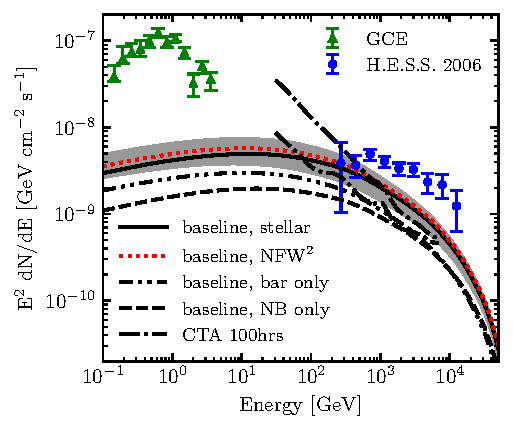
\includegraphics[width=\columnwidth]{Figures/IC_MSPs/ics_spectrum_hess_diffuse.pdf}
%   \caption{IC emissions from the Galactic ridge ($6^\circ\times 2^\circ$ area around the Galactic center). The fluxes from the baseline model for the stellar template (black solid) and NFW$^2$ template (red dotted) are shown. The shaded band represents the uncertainties due to the propagation parameters for the stellar template. The NB (dashed) and the Galactic bar (dot-dot-dashed) are shown separately for the baseline stellar model. Green triangles show the GCE data~\cite{2018NatAs...2..387M} and blue circles show the H.E.S.S. residuals~\cite{2006Natur.439..695A} in the Galactic ridge region. The upper dot-dashed (lower dot-dashed) line shows the CTA sensitivity for 100 hours from an ON-OFF analysis using the ring method toward the Galactic center with (without) systematic uncertainty considerations~\cite{2015JCAP...03..055S}. A dedicated morphological analysis could improve the shown sensitivities by up to a factor of $\sim 10$ \cite{2015JCAP...03..055S}.}
%   \label{fig:spectrum_diffuse}
% \end{figure}

\section{\label{sec:results_IC} Results}

Figure~\ref{fig:spectrum_diffuse} shows the predicted IC emissions from the Galactic ridge region (defined as the $6^\circ\times 2^\circ$ area around the Galactic center) for our stellar template (Galactic bar + NB). The solid black line is the expected flux from the baseline model. The shaded band represents the uncertainties resulting from changing the propagation setups as listed in Table~\ref{tab:dpara}. In the same plot we also show the expected flux from the NFW$^2$ template (red dotted), which is indistinguishable from that from the stellar template given the uncertainties from the propagation parameters. This conclusion also holds for larger regions of the bulge of interest ($20^\circ\times 20^\circ$ around the Galactic center). For the stellar template, we also show the IC emissions from the NB and the Galactic bar separately. For the Galactic ridge, the NB contributes $\sim 1/3$ of the total IC emission in the GeV energy range, and $\sim 1/2$ in the TeV range.

\begin{figure}[htb]
    \centering
    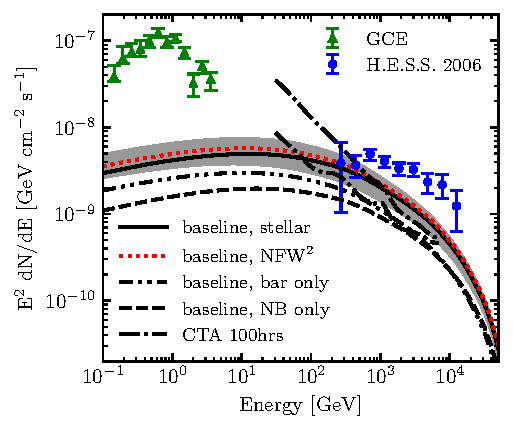
\includegraphics[width=0.7\textwidth]{Figures/IC_MSPs/ics_spectrum_hess_diffuse.pdf}
    \caption{IC emissions from the Galactic ridge ($6^\circ\times 2^\circ$ area around the Galactic center). The fluxes from the baseline model for the stellar template (black solid) and NFW$^2$ template (red dotted) are shown. The shaded band represents the uncertainties due to the propagation parameters for the stellar template. The NB (dashed) and the Galactic bar (dot-dot-dashed) are shown separately for the baseline stellar model. Green triangles show the GCE data~\cite{2018NatAs...2..387M} and blue circles show the H.E.S.S. residuals~\cite{2006Natur.439..695A} in the Galactic ridge region. The upper dot-dashed (lower dot-dashed) line shows the CTA sensitivity for 100 hours from an ON-OFF analysis using the ring method toward the Galactic center with (without) systematic uncertainty considerations~\cite{2015JCAP...03..055S}. A dedicated morphological analysis could improve the shown sensitivities by up to a factor of $\sim 10$ \cite{2015JCAP...03..055S}.}
    \label{fig:spectrum_diffuse}
\end{figure}

\begin{figure}[htb]
    \centering
    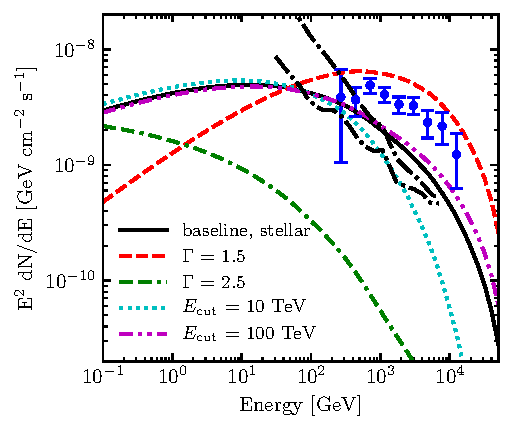
\includegraphics[width=0.7\textwidth]{Figures/IC_MSPs/ics_spectrum_hess_spectral.pdf}
    \caption{IC emissions for different $e^\pm$ spectra as listed in Table~\ref{tab:msp_spectrum}. H.E.S.S.~data and CTA sensitivities are shown in the same way as in Fig.~\ref{fig:spectrum_diffuse}, but note the different $y$ axis range.  Most spectra are below the H.E.S.S. measurements except for the hardest spectrum $\Gamma$ = 1.5 with $E_{\text{cut}}$ = 50 TeV which could be alleviated by a lower fraction of spin-down energy into relativistic $e^\pm$. For the soft spectrum $\Gamma$ = 2.5, the fluxes are below the CTA sensitivities by more than an order of magnitude.}
    \label{fig:spectrum_spectral}
\end{figure}
% \begin{figure}[t!]
%   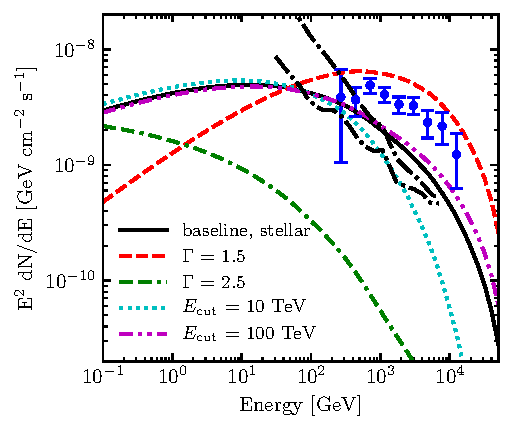
\includegraphics[width=\columnwidth]{Figures/IC_MSPs/ics_spectrum_hess_spectral.pdf}
%   \caption{IC emissions for different $e^\pm$ spectra as listed in Table~\ref{tab:msp_spectrum}. H.E.S.S.~data and CTA sensitivities are shown in the same way as in Fig.~\ref{fig:spectrum_diffuse}, but note the different $y$ axis range.  Most spectra are below the H.E.S.S. measurements except for the hardest spectrum $\Gamma$ = 1.5 with $E_{\text{cut}}$ = 50 TeV which could be alleviated by a lower fraction of spin-down energy into relativistic $e^\pm$. For the soft spectrum $\Gamma$ = 2.5, the fluxes are below the CTA sensitivities by more than an order of magnitude.}
%   \label{fig:spectrum_spectral}
% \end{figure}

The GCE data~\cite{2015MNRAS.451.1833M} at GeV energies, scaled to the Galactic ridge region, are shown by green triangles. The IC emission from MSPs is predicted to contribute less than $\sim 10$ \% of the GCE. This is consistent with previous works that have not found evidence for secondary emission at the $\sim 1$ GeV energy range~\cite{2016PhRvD..93j3004L}. The IC fluxes extend to the TeV energy range before decreasing steeply at $\sim 10$ TeV. Meanwhile the predicted fluxes are below or within the range of H.E.S.S.~observations (blue circles)~\cite{2006Natur.439..695A}. Our resolution does not probe the smaller-scales of $0.2^\circ$--$0.5^\circ$ investigated in Ref.~\cite{2018PhRvD..98d3005H}. Also shown in the same figure are the differential sensitivities for 100 hours of CTA diffuse Galactic center observations~\cite{2015JCAP...03..055S} (dot-dashed black lines). We note that our predicted IC fluxes could be detected by forthcoming CTA observations. Reference~\cite{2015JCAP...03..055S} computed the CTA sensitivities to a DM annihilation signal in the Galactic center. Although the spatial morphology considered in their work is different than ours, we use it as a representative of the CTA sensitivities to a large diffuse signal in this sky region. That work also showed that by performing dedicated morphological analyses, the sensitivity of CTA can be improved by up to an order of magnitude for DM annihilation signals. We expect that similar improvements could be obtained by performing such morphological analyses with the models considered in our current study.

% \begin{figure*}[t!]
% 	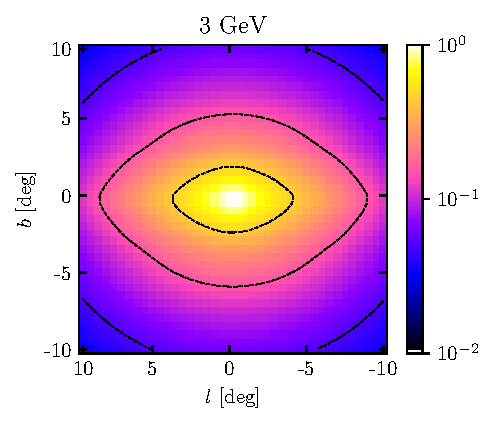
\includegraphics[width=0.68\columnwidth]{Figures/IC_MSPs/skymap_bulge_3gev.pdf}
%     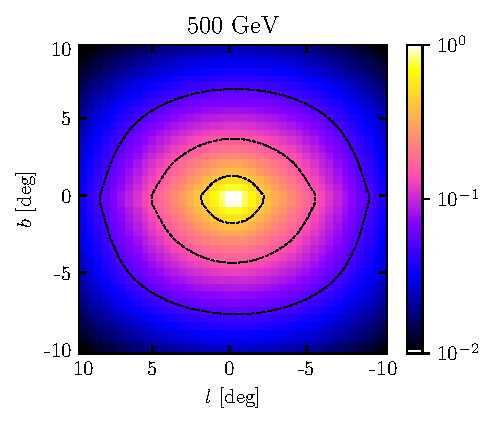
\includegraphics[width=0.68\columnwidth]{Figures/IC_MSPs/skymap_bulge_500gev.pdf}
%      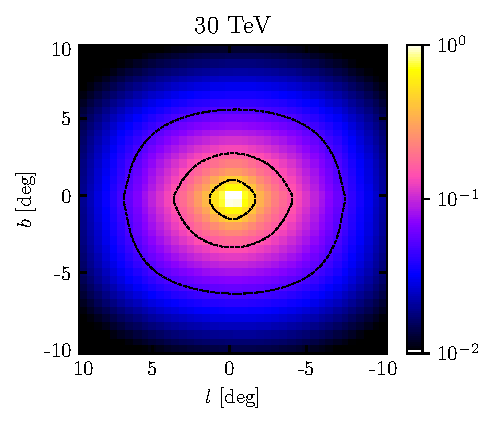
\includegraphics[width=0.68\columnwidth]{Figures/IC_MSPs/skymap_bulge_30tev.pdf}
%     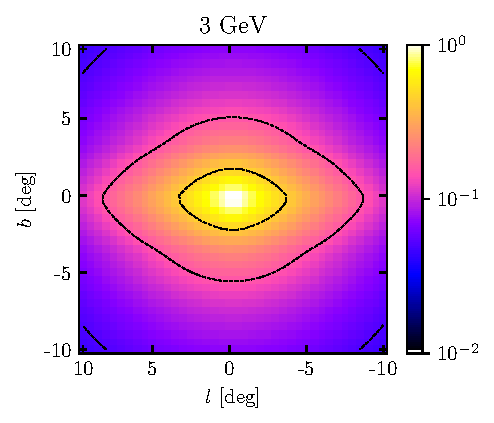
\includegraphics[width=0.68\columnwidth]{Figures/IC_MSPs/skymap_nfw_3gev.pdf}
%     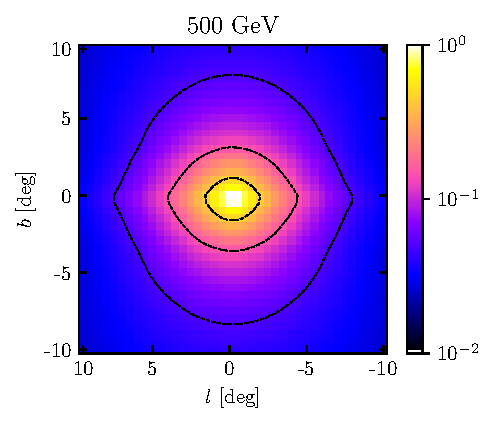
\includegraphics[width=0.68\columnwidth]{Figures/IC_MSPs/skymap_nfw_500gev.pdf}
%     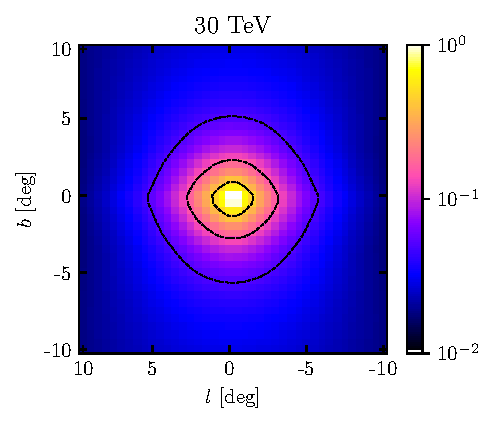
\includegraphics[width=0.68\columnwidth]{Figures/IC_MSPs/skymap_nfw_30tev.pdf}
%   \caption{IC sky maps from the baseline model for the stellar template (top row) and the NFW$^2$ template (bottom row) over a $20^\circ\times 20^\circ$ region around the Galactic center. Three energy windows are shown: 3 GeV (left column), 500 GeV (center column), and 30 TeV (right column). The injected $e^\pm$ are normalized by gamma-ray luminosities. The 5\%, 15\%, and 45\% flux levels with respect to the Galactic center are shown by dotted contours. The morphological differences between the stellar template and the NFW$^2$ template appear more prominently at high energies.}
%   \label{fig:skymap_bulge_vs_nfw}
% 	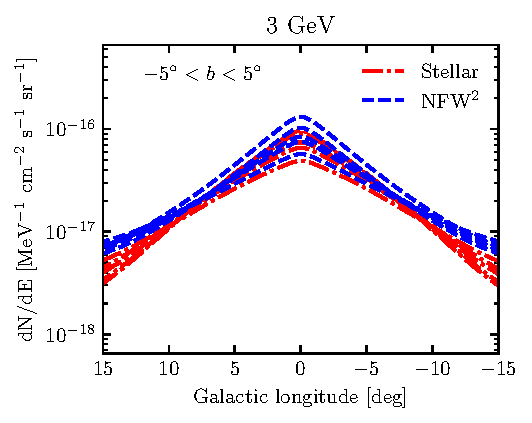
\includegraphics[width=0.68\columnwidth]{Figures/IC_MSPs/lon_3gev.pdf}
%     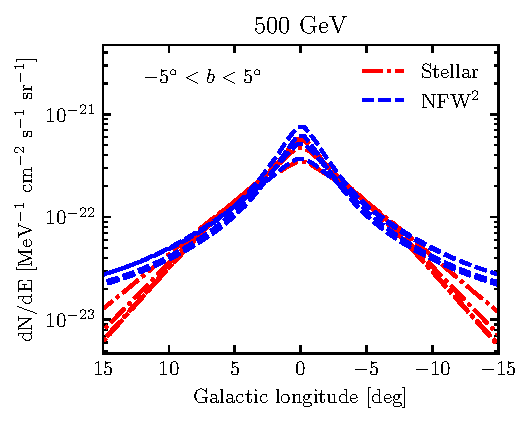
\includegraphics[width=0.68\columnwidth]{Figures/IC_MSPs/lon_500gev.pdf}
% 	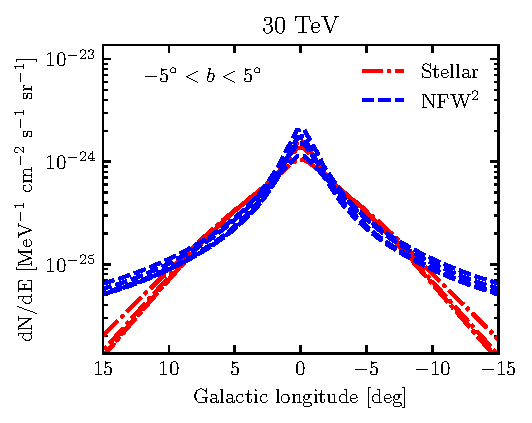
\includegraphics[width=0.68\columnwidth]{Figures/IC_MSPs/lon_30tev.pdf}
% 	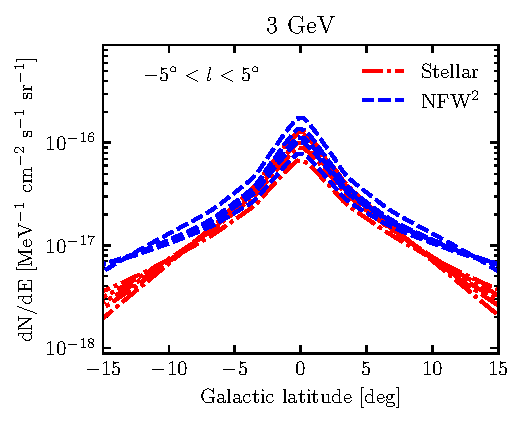
\includegraphics[width=0.68\columnwidth]{Figures/IC_MSPs/lat_3gev.pdf}
% 	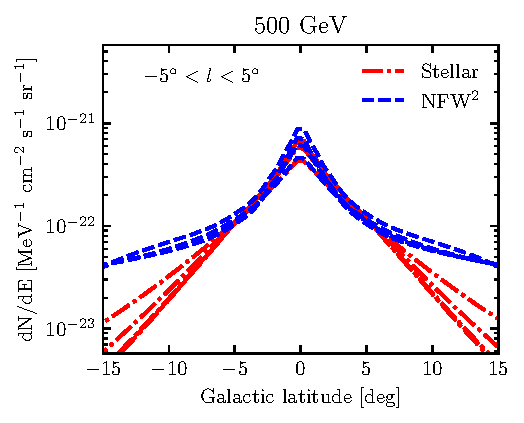
\includegraphics[width=0.68\columnwidth]{Figures/IC_MSPs/lat_500gev.pdf}
% 	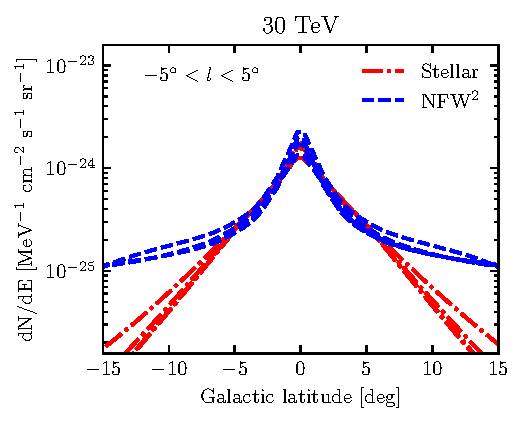
\includegraphics[width=0.68\columnwidth]{Figures/IC_MSPs/lat_30tev.pdf}
%   \caption{IC longitudinal (top row) and latitudinal (bottom row) profiles for the stellar template (red dot-dashed) and NFW$^2$ template (blue dashed), showing predictions from different propagation models as listed in Table~\ref{tab:dpara}.  The profiles are obtained by summing over 10$^\circ$ wide bands in the latitude and longitude directions, respectively. The columns are for the same energy windows as in Fig.~\ref{fig:skymap_bulge_vs_nfw}. The profiles show consistent changes in energy as seen in the corresponding sky map, and that the differences between the stellar and NFW$^2$ templates are greater than the differences caused by our selection of propagation setup.}
%   \label{fig:profile_bulge_vs_nfw}
% \end{figure*}

The IC spectra from the Galactic ridge region for different MSP injection spectra (Inj1, Inj2, ..., Inj4) are shown in Fig.~\ref{fig:spectrum_spectral}. We find that most of our predictions are at or below the corresponding H.E.S.S.~data points (assuming $f_{e^\pm} = 10\%$). However, for the hard injection spectrum model Inj1 ($\Gamma = 1.5$ and $E_{\text{cut}}=50$ TeV), the IC spectra overshoots the H.E.S.S.~observations. This means that either the Inj1 model is disfavored, or that $f_{e^\pm}$ is lower than $\sim 6\%$ in the Galactic ridge region. Contributing to this overshooting could be that the $e^\pm$ injection in the NB is overestimated. This is due to the fact that we normalize the $e^\pm$ luminosity by their gamma-ray luminosities. The best-fit NB gamma-ray luminosity obtained by Ref.~\cite{2018NatAs...2..387M} may be somewhat overestimated, because the NB spatial morphology is similar to that of the CMZ structure which could cause spatial degeneracies in the fits. In this sense, a fraction of the gamma-ray photons that are of hadronic origin (emitted by the CMZ) could have been absorbed by the NB stellar template. Also, we note that at around 100 TeV, pair production will attenuate the predicted flux by $\sim 3/4$.

Figure \ref{fig:skymap_bulge_vs_nfw} shows the morphologies of the IC emission for our baseline models in different energy windows: 3 GeV (left), 500 GeV (center), and 30 TeV (right). The top (bottom) row shows the sky maps for the stellar (NFW$^2$) template. The sky maps are normalized by their fluxes at the Galactic center. We find that there are energy-dependent morphological differences between the two IC predictions. These reflect the different $e^\pm$ source distribution models considered. In the GCE energy range ($\sim 3$ GeV, left panels), the IC sky maps are similarly elliptical for both the stellar and NFW$^2$ templates. However, the sky maps become less elliptical at 500 GeV and above. At around $\sim 30$ TeV, the morphologies of the IC component start to show the source distributions displayed in Fig.~\ref{fig:injection_skymap}. As it can be seen, in the highest energy window the sky maps for the stellar template (top-right panel) are boxy while that for the NFW$^2$ template (bottom-right panel) is close to spherical. However, the left-right asymmetry due to the tilt of the bar is not seen in the IC emissions.

\begin{figure}[htb]
    \centering
    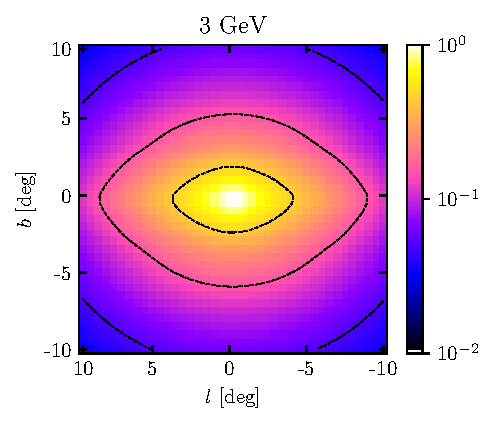
\includegraphics[width=0.3\textwidth]{Figures/IC_MSPs/skymap_bulge_3gev.pdf}
    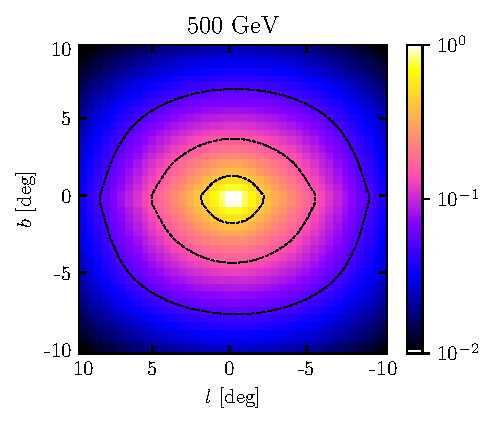
\includegraphics[width=0.3\textwidth]{Figures/IC_MSPs/skymap_bulge_500gev.pdf}
    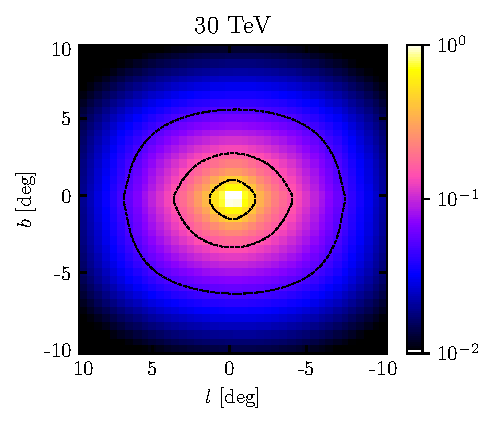
\includegraphics[width=0.3\textwidth]{Figures/IC_MSPs/skymap_bulge_30tev.pdf}
    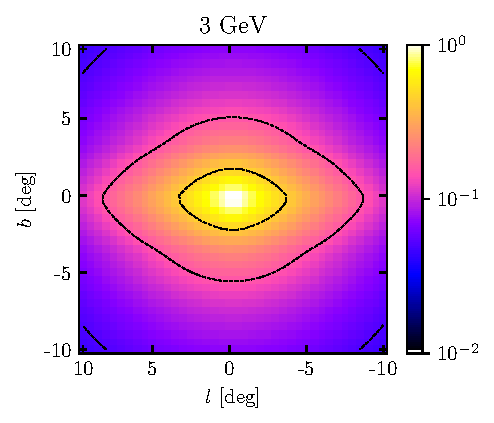
\includegraphics[width=0.3\textwidth]{Figures/IC_MSPs/skymap_nfw_3gev.pdf}
    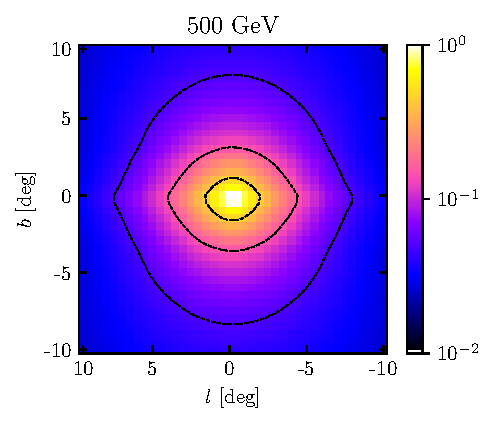
\includegraphics[width=0.3\textwidth]{Figures/IC_MSPs/skymap_nfw_500gev.pdf}
    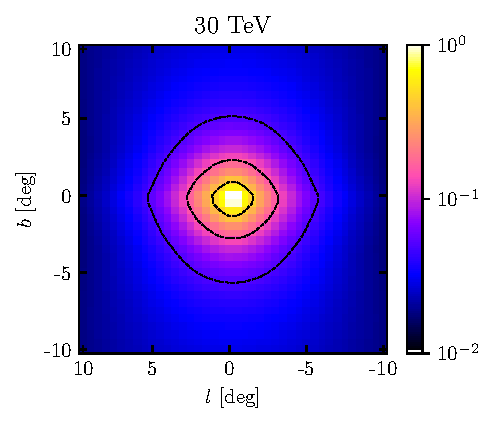
\includegraphics[width=0.3\textwidth]{Figures/IC_MSPs/skymap_nfw_30tev.pdf}
    \caption{IC sky maps from the baseline model for the stellar template (top row) and the NFW$^2$ template (bottom row) over a $20^\circ\times 20^\circ$ region around the Galactic center. Three energy windows are shown: 3 GeV (left column), 500 GeV (center column), and 30 TeV (right column). The injected $e^\pm$ are normalized by gamma-ray luminosities. The 5\%, 15\%, and 45\% flux levels with respect to the Galactic center are shown by dotted contours. The morphological differences between the stellar template and the NFW$^2$ template appear more prominently at high energies.}
    \label{fig:skymap_bulge_vs_nfw}
\end{figure}

These features can be seen more clearly in the corresponding latitudinal and longitudinal profiles presented in Fig.~\ref{fig:profile_bulge_vs_nfw}. Here, we also show the variations in predicted IC morphologies when the propagation setups are varied, as in Table~\ref{tab:dpara}. We note that the morphological differences between the stellar and NFW$^2$ templates are robust to changes in the propagation parameters. It is clear that at tens of TeV, the IC sky maps are sensitive to the source injection distributions.

\begin{figure}[htb]
    \centering
    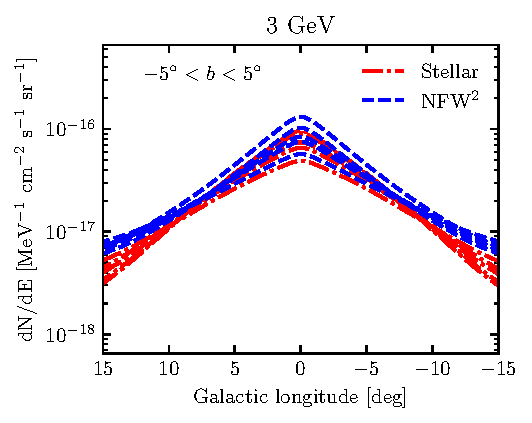
\includegraphics[width=0.3\textwidth]{Figures/IC_MSPs/lon_3gev.pdf}
    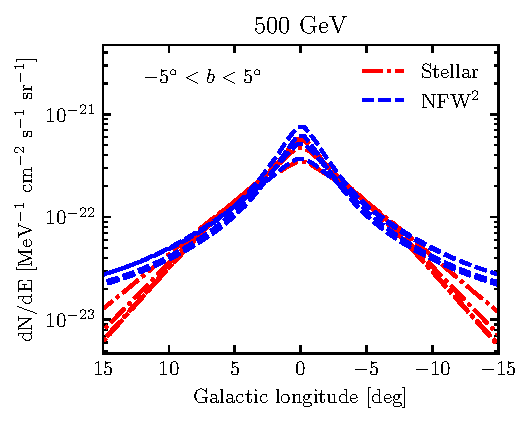
\includegraphics[width=0.3\textwidth]{Figures/IC_MSPs/lon_500gev.pdf}
    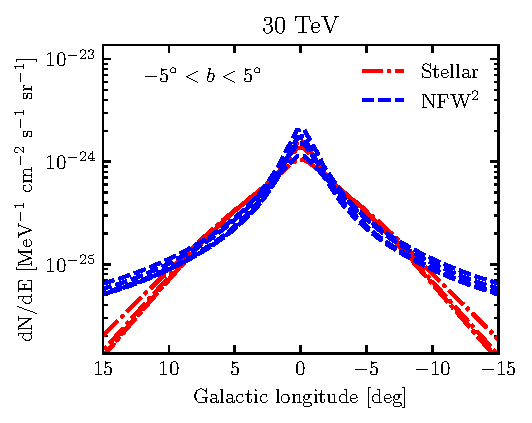
\includegraphics[width=0.3\textwidth]{Figures/IC_MSPs/lon_30tev.pdf}
    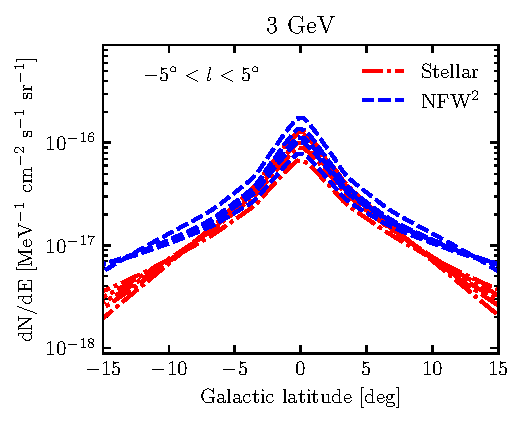
\includegraphics[width=0.3\textwidth]{Figures/IC_MSPs/lat_3gev.pdf}
    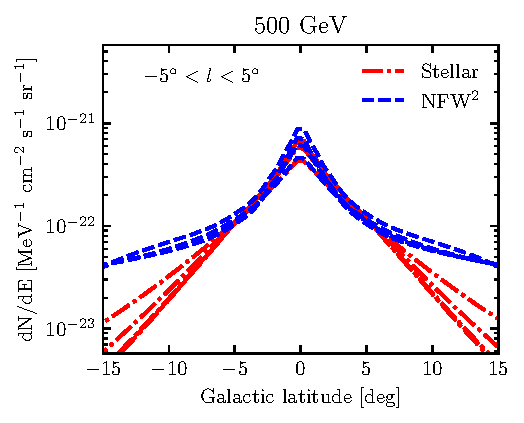
\includegraphics[width=0.3\textwidth]{Figures/IC_MSPs/lat_500gev.pdf}
    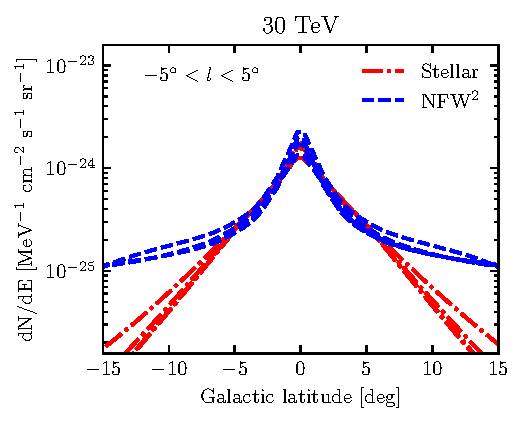
\includegraphics[width=0.3\textwidth]{Figures/IC_MSPs/lat_30tev.pdf}
    \caption{IC longitudinal (top row) and latitudinal (bottom row) profiles for the stellar template (red dot-dashed) and NFW$^2$ template (blue dashed), showing predictions from different propagation models as listed in Table~\ref{tab:dpara}.  The profiles are obtained by summing over 10$^\circ$ wide bands in the latitude and longitude directions, respectively. The columns are for the same energy windows as in Fig.~\ref{fig:skymap_bulge_vs_nfw}. The profiles show consistent changes in energy as seen in the corresponding sky map, and that the differences between the stellar and NFW$^2$ templates are greater than the differences caused by our selection of propagation setup.}
    \label{fig:profile_bulge_vs_nfw}
\end{figure}

At IC photon energies of $\sim 1$ GeV, the IC emission is in the nonrelativistic (Thomson) regime and the IC flux is dominated by up-scattered optical photons (Fig.~\ref{fig:spectrum_comp}). The optical photons are mainly emitted by stars whose density peaks along the Galactic plane. As a result, in this energy range the IC emissions are elongated along the Galactic plane and have marked elliptical appearances. This is almost invariant of the spatial morphology of the MSP distributions assumed, explaining the similarity between the left panels of Fig.~\ref{fig:skymap_bulge_vs_nfw}. However, at higher energies, the IC emission starts to enter the relativistic scattering (Klein-Nishina) regime and becomes suppressed, causing the decline of the up-scattered optical photon signal from around 100 GeV (red dotted curve in Fig.~\ref{fig:spectrum_comp}). Since the Klein-Nishina regime is reached at higher energies for lower-energy target photons~\cite{2014ApJ...793...64A}, the IR and CMB photons continue, overtaking the optical photons. Furthermore, as the IR is less concentrated along the Galactic plane than the optical photons (and the CMB is isotropic), the IC emission retains more morphological information of the injected $e^\pm$.

\begin{figure}[htb]
    \centering
    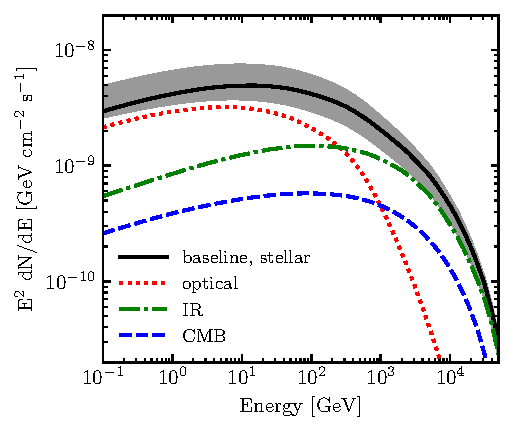
\includegraphics[width=0.7\textwidth]{Figures/IC_MSPs/ics_spectrum_components.pdf}
    \caption{Components of the IC emission for the baseline stellar model from the Galactic ridge, arising from different up-scattered photon fields: optical (red dotted), IR (green dot-dashed), CMB (blue dashed), and the total (black solid). The optical component dominates the GeV energy range, but decreases above 100 GeV, eventually being overtaken by up-scattered IR and CMB photons.}
    \label{fig:spectrum_comp}
\end{figure}

A larger magnetic field means greater energy loss due to synchrotron radiation of the injected $e^\pm$ and a corresponding reduction in the IC emission. We tested a constant magnetic field $B = 50\ \mu$G in the Galactic center region on scales of 400 pc (see Sec.~\ref{sec:bfield}) to explore its impact on our model predictions. Figure~\ref{fig:spectrum_bfields} shows the predicted IC spectrum for the baseline model assuming the default magnetic field (black solid curve with gray shaded band) and the corresponding IC spectrum for the same model but assuming the modified magnetic field (red solid curve). As can be seen, the IC spectrum normalization for the enhanced magnetic field setup is $\sim 1/2$ of the default one. This represents a change in normalization that is larger than our estimated modeling uncertainties from different propagation models (gray shaded). This reduction is mainly due to synchrotron energy loss of $e^\pm$ in the NB. Figure~\ref{fig:spectrum_bfields}  displays the predicted IC spectrum for the NB component (red dashed curve) and Galactic bar (red dot-dot-dashed curve) separately in the enhanced magnetic field case. We observe that for this case the Galactic bar emission dominates. This is different to our predictions obtained using the default magnetic field setup, where the NB and bar  contributions were comparable (see Fig.~\ref{fig:spectrum_diffuse}). This can be understood by noticing that the NB resides in the region where the modified magnetic field underwent the normalization increase. Consequently, much of the $e^\pm$ emitted from this region endure maximum energy loss via synchrotron radiation.

\begin{figure}[htb]
    \centering
    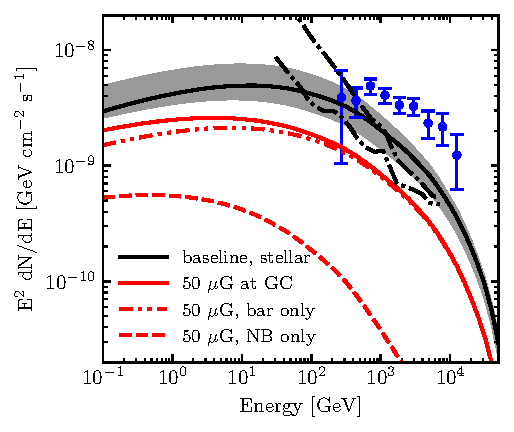
\includegraphics[width=0.7\textwidth]{Figures/IC_MSPs/ics_spectrum_bfields.pdf}
    \caption{IC emissions from different magnetic field models. The baseline (black solid curve) adopts the original \textsc{galprop} magnetic field. The red solid curve introduces a 50 $\mu$G lower limit for the inner 400 pc region around the Galactic center. With the presence of such a lower limit, the IC emission from the Galactic ridge is reduced by $\sim 1/2$. Due to the higher overlap with the modified magnetic field, the IC emission from the NB (red dashed curve) is suppressed more strongly by synchrotron loss compared to the Galactic bar (red dot-dot-dashed curve).}
    \label{fig:spectrum_bfields}
\end{figure}

\section{\label{sec:conclu}Discussion and Conclusion}

Recent analyses of the GCE~\cite{2018NatAs...2..387M,2018NatAs...2..819B,2019JCAP...09..042M} have revealed its nonspherical nature and have provided further support for an MSP origin. We have revisited the computation of secondary IC emission from the $e^\pm$ injected by such MSPs. Compared to previous studies that assumed a spherically symmetric spatial distribution of MSPs, we adopted 3D models of the stellar distributions in the Galactic center and numerically calculated the IC emissions using the {\tt GALPROP} code. Furthermore, we systematically explored the impact of diffusion parameter uncertainties with additional {\tt GALPROP} runs. We found that the predicted IC fluxes beyond 100 GeV are within the forecasted sensitivity limits of future gamma-ray telescopes for our baseline parameters (Fig.~\ref{fig:spectrum_diffuse}). The very high-energy IC emission from MSPs is nondegenerate with that caused by DM annihilation, from which the $e^\pm$ can only reach a few tens of GeV if DM is responsible for the GCE.

Although the IC spectra from the Galactic center provide insufficient information for identifying the spatial model of the source, we found that the spatial morphology of the IC could serve as a discriminant between the spherically symmetric and 3D stellar distribution injection models (Fig.~\ref{fig:skymap_bulge_vs_nfw}). In the GeV energy range, the IC morphologies are equally elliptical for both the stellar and NFW$^2$ models. However, above $\sim$ TeV energies, they reveal morphological differences that trace the injection distributions. They can therefore be used to discriminate the spherically symmetric and 3D stellar injection models.

Our predicted IC fluxes contribute $\lesssim 10 \%$ of the GCE emission and are at or below than the H.E.S.S.~observations of the Galactic ridge at around a  few TeV. These are consistent with the null detection of secondary emissions in the GeV range \cite{2016PhRvD..93j3004L} and the dominantly hadronic origins of the H.E.S.S.~measurements ~\cite{2017PhRvL.119c1101G,2016Natur.531..476H}. Thus they constitute important consistency checks of the MSP scenario for the GCE. We compared the IC fluxes with the CTA sensitivity from Ref.~\cite{2015JCAP...03..055S} and found that the IC emission could be detected and potentially reveal a signature of Galactic center MSPs with a specialized spectral and morphological search. The HAWC telescope~\cite{2012NIMPA.692...72D,2013arXiv1310.0074H} operates in similar energy bands, and while not having a full view of the Galactic bulge region may have sensitivity to hard $e^\pm$ injection models. To this end, a wide field-of-view TeV gamma-ray observatory in the southern hemisphere is warranted \cite{2017ICRC...35..851M}.

The detectability of the IC emission depends on the setup, including MSP $e^\pm$ spectrum and propagation parameters. We adopted a canonical $e^\pm$ power-law slope of 2.0, but softer spectra would make it a challenge to detect the IC component at TeV energies (Fig.~\ref{fig:spectrum_spectral}). Furthermore, an increased magnetic field at the Galactic center would reduce the IC emission via enhanced synchrotron energy losses. In particular, assuming a constant magnetic field of magnitude 50 $\mu$G in the inner 400 pc of the Galactic center, we found a reduction of $\sim 1/2$ of the IC emission obtained with the default magnetic field setup. On the other hand, our model predictions were not very sensitive to changes in the propagation parameters within the 95\% credible contours provided in the 2D marginalized posterior distributions of Ref.~\cite{2016ApJ...824...16J}.

There are various assumptions in our calculations that warrant future detailed studies. For example, we used the default ISRF from the {\tt GALPROP} version 54, which is 2D after averaging the angular dependence. This has recently been updated in Refs.~\cite{2017ApJ...846...67P,2018ApJ...856...45J}, where a 3D ISRF was adopted in the context of CR propagation and high-energy gamma-ray emissions in the Galaxy. Their results show nontrivial impacts from employing the 3D ISRF on the propagation parameters of CRs and the gamma-ray intensity maps. Our results may be affected in many ways, including the fluxes and sky maps. Studies with the {\tt PICARD} code show that new ISRFs increase gamma-ray intensities from the Galactic center, in particular at energies of $\sim 200 $ GeV \cite{2019APh...107....1N}. Note however that our Galactic bar parametrization remains consistent with the ISRF of \textsc{galprop}. Even though more recent analyses suggest a larger tilt angle, we found that the left-right bulge asymmetry caused by the tilt is washed out in the IC sky maps, and is certainly smaller than the uncertainty caused by propagation parameters.

For the propagation part, we have adopted the results of a wide scan of propagation parameters \cite{2016ApJ...824...16J}. However, caution must be exercised since the propagation properties around the Galactic center may be unique. We also have not covered all possibilities, e.g., we did not consider the possibility of cosmic rays advected out of the region by large-scale outflows. Such outflows may be related to the Fermi bubbles \cite{2015ApJ...808..107C} and depending on the velocity would affect the secondary IC morphology. We have also neglected MSPs in the Galactic disk, which would provide additional $e^\pm$ injection and IC emission. However, population syntheses show that the MSP contribution to the Galactic diffuse gamma-ray emission is at the few-percent level or less \cite{2018ApJ...863..199G} and we do not expect this to substantially affect our results.

We have modeled the MSP population in the Galactic bulge. However, the presence of younger pulsars and the evolution of the pulsar population were not considered. It has been shown that TeV halos from younger pulsars can contribute to TeV emissions~\cite{2018PDU....21...40H}. This may potentially change the spectral property of IC emissions from the NB where active star formation is ongoing.

The magnetic field at the Galactic center is a crucial parameter affecting the IC emission from a putative MSP population in the nuclear bulge. We have shown that an enhanced magnetic field in this region in turn augments the synchrotron energy losses of the MSP $e^\pm$, thus decreasing the IC yields. The estimated magnetic fields at $\sim$ 100 pc around the Galactic center has large uncertainties and vary from 10 $\mu$G~\cite{2005ApJ...626L..23L} to 1000 $\mu$G~\cite{1989ApJ...343..703M}. Here we only tested the original \textsc{galprop} model ($\sim 10\ \mu$G at the Galactic center) and a 50 $\mu$G lower limit obtained in Ref.~\cite{2010Natur.463...65C}. An even larger magnetic field at the Galactic center means that the synchrotron radiation would be dominant, especially for the NB component that resides within the 230 pc region around the Galactic center. The spectrum and morphology of the IC emission from the Galactic ridge would potentially be changed by a strong magnetic field in this region. However, the effects on the larger-scale bar/bulge component are expected to be minor. On the other hand, we have only considered the 2D random magnetic field component. A recent study~\cite{2019PhRvD..99d3007O} showed that the IC spatial maps can be significantly affected when more realistic 3D magnetic fields with both random and ordered components are included. This will apply also in the context of MSP secondary emission but its investigation is beyond the scope of the current study.

The Galactic center of the Milky Way offers a unique window to study novel astrophysical and dark matter signals. We have shown that the TeV energy range offers a new handle on the morphology of putative MSPs in the Galactic bulge responsible for the GeV excess. Telescopes such as CTA and HAWC South can be helpful for detecting these IC emissions and for constraining the origin of the GCE in the future.

\section*{Acknowledgments}
We thank Roland Crocker for careful reading of the manuscript and insightful suggestions. We thank Kev Abazajian and  Manoj Kaplinghat for comments on the manuscript. DS and SH are supported by the U.S.~Department of Energy under award number de-sc0018327. This work was partially supported by World Premier International Research Center Initiative (WPI Initiative), MEXT, Japan. OM acknowledges support by JSPS KAKENHI Grant Numbers JP17H04836, JP18H04340 and JP18H04578. The authors acknowledge Advanced Research Computing at Virginia Tech for providing computational resources and technical support that have contributed to the results reported within this paper. URL: \url{http://www.arc.vt.edu}

\chapter{Cherenkov Telescope Array sensitivity to Galactic center millisecond pulsars}\label{ch:CTA}
% Cherenkov Telescope Array sensitivity to the putative millisecond pulsar population responsible for the Galactic center excess

\section{Abstract}

The leading explanation of the \textit{Fermi} Galactic center $\gamma$-ray excess is the extended emission from a unresolved population of millisecond
pulsars (MSPs) in the Galactic bulge. Such a population would, along with the prompt $\gamma$ rays, also inject large quantities of electrons/positrons ($e^\pm$) into the interstellar medium. These $e^\pm$ could potentially inverse-Compton (IC) scatter ambient photons into $\gamma$ rays that fall within the sensitivity range of the upcoming Cherenkov Telescope Array (CTA). In this article, we examine the detection potential of CTA to this signature by making a realistic estimation of the systematic uncertainties on the Galactic diffuse emission model at TeV-scale $\gamma$-ray energies. We forecast that, in the event that $e^\pm$ injection spectra are harder than $E^{-2}$, CTA has the potential to robustly discover the IC signature of 
a putative Galactic bulge MSP population sufficient to explain the GCE for $e^\pm$ injection efficiencies in the range $\approx 2.9$--74.1\%, or higher, depending on the level of mismodeling of the Galactic diffuse emission components. On the other hand, for spectra softer than $E^{-2.5}$, a reliable CTA detection would require an unphysically large $e^\pm$ injection efficiency of $\gtrsim 158\%$. However, even this pessimistic conclusion may be avoided in the plausible event that
MSP observational and/or modeling uncertainties can be reduced. We further find that, in the event that an IC signal were detected, CTA can successfully discriminate between an MSP and a dark matter origin for the radiating $e^\pm$.

\section{Attribution}

This chapter is based on the following publication to which I have contributed:
\begin{itemize}
    % \item \emph{Song, D., Macias, O., and Horiuchi, S., “Inverse Compton emission from millisecond pulsars in the Galactic bulge”, Physical Review D, vol. 99, no. 12, 2019}
    \item \emph{Macias, O., van Leijen, H., Song, D., Ando, S., Horiuchi, S., and Crocker, R. M., “Cherenkov Telescope Array sensitivity to the putative millisecond pulsar population responsible for the Galactic Centre excess”, Monthly Notices of the Royal Astronomical Society, vol. 506, no. 2, 2021}
    % \item \emph{Song, D., Macias, O., Horiuchi, S., Crocker, R. M., and Nataf, D. M., “Evidence for a high-energy tail in the gamma-ray spectra of globular clusters”, Monthly Notices of the Royal Astronomical Society, vol. 507, no. 4, 2021}
    % \item \emph{Siegert T., Crocker R.~M., Macias O., Panther F.~H., Calore F., Song D., Horiuchi S, “Measuring the smearing of the Galactic 511 keV signal: positron propagation or supernova kicks?”, Monthly Notices of the Royal Astronomical Society Letters, accepted for publication, 2021}
\end{itemize}
Oscar Macias led the collaboration. I improved the calculation of the IC signals using the \textsc{galprop} v56. Oscar Macias and Harm van Leijen did the CTA sensitivity estimate based on the improved IC maps. Oscar and I calculated the predicted $e^\pm$ injection efficiencies. Shin'ichiro Ando and Shunsaku Horiuchi contributed to the interpretation of the results.


\section{Introduction}
\label{sec:introduction}


\textit{Fermi} Large Area Telescope (LAT) observations~\citep{2011PhLB..697..412H,2011JCAP...03..010A,2012PhRvD..86h3511A,2013PhRvD..88h3521G, 2014PhRvD..89f3515M,2015JCAP...03..038C,2016PDU....12....1D,2016ApJ...819...44A,2017ApJ...840...43A} of the inner $\sim 10^{\circ}$ of the Galactic center region have revealed extended  gamma-ray emission in significant excess with respect to the astrophysical background model. Early studies of this ``Galactic center excess'' (GCE) appeared to show the signal to be spherically symmetric around the Galactic center with a radially-declining intensity. This, together with the fact that the GCE is described by a 
spectral energy distribution peaked at a few GeV,
led to the possibility that it
originates from
self-annihilation of  weakly interacting massive particles (WIMPs) spatially distributed 
according to something approaching (actually somewhat steeper than)
a Navarro-Frenk-White (NFW) density profile 
\citep{2011PhLB..697..412H,2012PhRvD..86h3511A,2013PhRvD..88h3521G}. However, recent reanalyses of the spatial morphology of the GCE~\citep{2018NatAs...2..387M,2018NatAs...2..819B,2019JCAP...09..042M, 2020PhRvD.102d3012A} have demonstrated that its spatial morphology is better described by the (non-spherically symmetric) stellar density distribution of the Galactic bulge than by profiles expected for the WIMP annihilation. The Galactic bulge hosts a large variety of stellar populations from old to 
recently-formed
\citep{1997ApJ...491L..31G,2000MNRAS.317L..45H}, and should contain many 
types of
gamma-ray sources, 
the prime example of which is the expected large population of millisecond pulsars (MSPs)~\citep{2011JCAP...03..010A,2012PhRvD..86h3511A,2013PhRvD..88h3521G,2017JCAP...08..015P, 2018MNRAS.475.5313F, 2018MNRAS.480.4955F, 2018ApJ...863..199G, 2020JCAP...12..035P}---old pulsars that have been spun-up due to their
interaction within a binary system.

In particular, \citet{2020PhRvD.102d3012A} performed a reanalysis of the GCE and demonstrated that, when including maps tracing stellar mass in the Galactic and nuclear bulges, the Galactic center shows no significant detection of a dark matter (DM) annihilation signal. These results were shown to be robust to generous variations of the astrophysical backgrounds (e.g., combinations of two-dimensional or three-dimensional inverse Compton maps, interstellar gas maps, a central source of electrons) and DM morphologies (e.g., cored DM profiles, generalized NFW, and ellipsoidal versions of these). This allowed some of us to obtain very strong constraints on DM properties. Interestingly, the key result that the spatial morphology of the GCE is better described by a stellar bulge template than by a NFW model has been recently confirmed by an updated analysis with SkyFACT~\citep{2021PhRvL.127p1102C}. Though we notice that~\citet{2021PhRvD.103f3029D} obtained otherwise.

Several recent studies~\cite[e.g.,][]{2016PhRvL.116e1103L,2016PhRvL.116e1102B, 2019PhRvL.123x1101L,2018PhRvD..98d3009B,2020PhRvD.101b3014C,2020PhRvD.102f3019L,2020PhRvL.125l1105L,2020PhRvD.102b3023B,2021PhRvL.127p1102C} have also proposed different methods to resolve the source nature of the GCE. Although there is no consensus yet in the community regarding the main results of such methods~\cite[e.g.,][]{2020PhRvD.102f3019L,2020PhRvL.125l1105L,2020PhRvD.102b3023B,2016PhRvL.116e1102B,2018PhRvD..98d3009B}, it should be noted that these studies are probing the photon-count statistics of the GCE, which is an aspect of the signal that is independent of the morphological analyses and results in~\citep{2018NatAs...2..387M,2018NatAs...2..819B, 2019JCAP...09..042M}. Indeed, the spectrum and spatial morphology are the most basic characteristics of the gamma-ray sources in the sky~\citep{2020ApJS..247...33A}, and these two characteristics of the GCE are in strong agreement with a Galactic bulge explanation of the GCE~\cite[e.g.,][]{2020PhRvD.102d3012A}. 

Pulsars have long been predicted to be sources of electron-positron ($e^{\pm}$) pairs~\citep{1966RvMP...38..626E,1970Natur.227..465S,1971ApJ...164..529S, 1995A&A...294L..41A, 1995PhRvD..52.3265A}. Highly energetic $e^{\pm}$ in the wind regions or inner magnetospheres of pulsars, 
also when released into the general interstellar medium,
can inverse-Compton (IC) scatter ambient photons to very high energies. 
The recent HAWC~\citep{2017Sci...358..911A} observations of extended TeV-scale gamma-ray emission around Geminga and Monogem have provided indirect evidence for TeV $e^{\pm}$ acceleration in normal pulsar nebulae.  Since a multitude of normal pulsars have been observed in the vicinity of the solar system, they have been purported~\citep{2009JCAP...01..025H, 2010A&A...524A..51D,2017Sci...358..911A,2017PhRvD..96j3013H, 2018PhRvD..97l3008P,2019PhRvD.100l3015D, 2019ApJ...879...91J} as the likely source of the majority of local cosmic ray positrons~\citep{2013PhRvL.110n1102A}.    
Several lines of evidence also point to potentially efficient $e^{\pm}$ acceleration by MSPs. First, a recent study~\citep{2021PhRvD.103h3017S} of the correlation between far-infrared and radio luminosities in star-forming galaxies (SFGs) found that radio emission from MSPs may account for a large fraction of the radio luminosity observed in systems with high stellar mass but low star formation rate. 
%
In particular, the unexpectedly high radio luminosities of such
systems
might be explained by the cooling of GeV-scale $e^{\pm}$ from MSPs via synchrotron radiation in each host galaxy's interstellar medium (ISM). Second, ~\citet{2021MNRAS.507.5161S} have found evidence for IC emission produced by MSP populations in globular clusters of the Milky Way. Furthermore, the H.E.S.S. telescope has observed extended TeV gamma-ray emission from the direction of the globular cluster Terzan 5~\citep{2013A&A...551A..26H}. Such gamma-rays could naturally arise from Comptonization of the background radiation within the globular cluster by super-TeV $e^{\pm}$~\citep{2016MNRAS.458.1083B}. 
%
Note that while a similar search conducted by H.E.S.S in another 15 globular clusters~\citep{2013A&A...551A..26H}, and MAGIC in the M15 globular cluster~\citep{2019MNRAS.484.2876M}, only produced gamma-ray flux upper limits, it seems likely that forthcoming gamma-ray instruments could resolve a large number of globular clusters at TeV energies~\citep{2018MNRAS.473..897N,2021MNRAS.500.4827N}. 
Third, several analyses of the GCE~\citep[e.g.,][]{2016JCAP...11..053H,2016PhRvD..94j3013L,2021PhRvD.103f3029D} have found evidence for a high-energy tail, possibly related to IC emission from $e^\pm$ accelerated by the sources responsible for it. 
%
Finally, recent simulation work \citep{2020A&A...635A.138G} suggests that MSPs could efficiently accelerate $e^{\pm}$ pairs to TeV-scale energies and beyond. 

In this chapter, we propose that the hypothesized population of approximately 20 to 50 thousand MSPs~\citep{2020JCAP...12..035P} in the Galactic bulge, could inject large numbers of highly energetic $e^{\pm}$ into the ISM~\footnote{Note that other studies~\citep[e.g.,][]{2018JCAP...07..042G} have explored the proton signatures from Galactic center MSPs.}. The  IC signal resulting from these could be detectable~\citep{2019PhRvD..99l3020S} by planned TeV-scale gamma-ray telescopes such as 
the Cherenkov Telescope Array (CTA). 
%
In particular, CTA will observe the center of the Milky Way with unprecedented spectral and spatial detail~\citep{2019scta.book.....C}. 
%
CTA's anticipated strategy for a survey of the inner Galaxy entails a deep exposure observation of the inner few degrees of the Galactic center region plus an extended survey covering a large fraction of the northern side of the Galactic bulge ($|l|\lesssim 6^{\circ}\;{\rm and}\; 0.3^{\circ}\lesssim b \lesssim 10^{\circ}$). The latter will facilitate the study of diffuse very high energy (VHE) sources such as Galactic outflows (a possible VHE counterpart to the Fermi bubbles), interstellar gas-correlated gamma-ray emission, a potential DM emission signature~\citep{2021JCAP...01..057A}, unresolved gamma-ray sources~\citep{2019ICRC...36..817V}, and, as we will thoroughly explore here, the IC emission from the 
population of $e^\pm$ launched into the bulge ISM by the
 MSPs putatively responsible for the GCE.  



Recently,~\citet{2019PhRvD..99l3020S} performed detailed simulations (using \textsc{galprop} V54~\citealt{2006ApJ...648L..29P}) of the IC signature from the putative population of MSPs responsible for the GCE. Compared to that work, here we recompute all our spatial maps using the latest version of the code (\textsc{galprop} V56)---which contains new three-dimensional (3D) models for the interstellar radiation fields, Galactic structures, and interstellar gas maps. Furthermore, now we run our simulations in the 3D mode of the \textsc{galprop} framework, abandoning the assumption of Galactocentric cylindrical symmetry. Interestingly, \cite{2019PhRvD..99l3020S} argued that it could be possible for CTA to (i) detect the population of MSPs responsible for the GCE, and (ii) distinguish whether the IC signal emanates from either DM self-annihilation or these unresolved MSPs in the Galactic bulge. 

Here, we perform a realistic assessment of the sensitivity of CTA to such an unresolved population of MSPs in the Galactic center. Using simulated data, we consider scenarios where the Galactic diffuse emission (GDE) is known accurately, as well as cases where the GDE is mismodeled. In each case, we investigate the necessary conditions for a reliable CTA detection of the MSPs' IC signal. Similarly, we study whether CTA could separate the nature of the source producing the IC emission. As shown in~\citet{2019PhRvD..99l3020S}, the expected IC emission from the Galactic bulge MSPs has morphological differences with respect to the one from DM emission. We now present a systematic study on simulated data that takes into account the latest CTA instrument response function and state-of-the-art models for the GDE to fully address these points.
 
This chapter is organized as follows. In Sec. \ref{sec:ICfromMSPs} we describe the procedure used to construct the TeV-scale IC flux maps produced by the putative MSP population responsible for the GCE. In Sec.~\ref{sec:backgroundtemplates}, we present the astrophysical backgrounds in the Galactic center region that are relevant for the IC searches. In Sec.~\ref{sec:sensitivity} we provide an overview of the expected CTA performance, the expected background and signal rates, and the methodology to estimate the CTA sensitivity. We present our results in Sec.~\ref{sec:results_CTA}, and the discussion and conclusions in Sec.~\ref{sec:discussions_CTA}. 
 
 

\section{Computation of IC emission from MSPs in the Galactic Center}
\label{sec:ICfromMSPs}


\subsection{Production mechanisms of $e^{\pm}$ pairs in millisecond pulsars}
\label{subsec:e+-injection}

Millisecond pulsars are neutron stars with high rotation rates (spin periods in the range of tens of ms or less) and relatively low surface magnetic fields ($\sim 10^{8}$ G). Due to their very rapid rotation, MSPs can produce high  
electric fields and spin-down power. Despite their low surface magnetic fields, their very compact magnetospheres allow for 
magnetic fields at the light cylinder that are comparable to those of normal pulsars~\citep{2021arXiv210105751H}. Their observed pulsed emission---as seen by an observer located inside the cone scanned by the magnetic field---is explained by the misalignment of the pulsar rotation axis and the magnetic field axis.  If the neutron star surface temperature ($T_s$) is greater than the electron surface binding temperature (i.e., $T_s\gtrsim 10^5$ K), then electrons can be torn from the neutron star surface by the strong electric fields~\citep{1991tnsm.book.....M}. Such electrons would subsequently move parallel to magnetic field lines and emit gamma-ray photons through curvature radiation. An additional large number of ``secondary'' electrons (and positrons) can be created through pair production processes at different sites throughout the MSPs magnetosphere. 
Dedicated phenomenological studies of MSPs demonstrate that most of their high-energy emission occurs near the current sheet outside the light cylinder~\citep{2020ApJS..247...33A,2021arXiv210105751H}.
Furthermore, in global magnetosphere models, charge currents, electromagnetic fields, and current sheets scale with the light cylinder independent of the pulsar surface magnetic field strength or rotation period. Thus, new emission models of MSPs predict high energy radiation that is similar to that of normal pulsars (the reader is referred to~\citealt{2021arXiv210105751H} for further details).

\subsection{Spatial distribution of the MSP population in the Galactic Center}
\label{subsec:spatialdistribution}

A very interesting implication of recent GCE analyses~\citep{2018NatAs...2..387M,2018NatAs...2..819B,2019JCAP...09..042M,2020PhRvD.102d3012A}, is that prompt gamma-ray emission from MSPs in the Galactic bulge could account for the bulk of the GCE emission~\citep{2012PhRvD..86h3511A}. Since 
prompt emission occurs within or very close to the magnetospheres of individual MSPs and
gamma rays travel following geodesics in space-time, the spatial morphology of the GCE can be used to map the spatial distribution of this putative MSP population.

Here, we follow the same approach as \cite{2019PhRvD..99l3020S} who assumed that the MSP population is smoothly distributed following the density of stars in the Galactic bulge (see Sec.~\ref{subsec:disentanglingMSPsfromDM}). In particular, the Galactic bulge consists of two main components: the nuclear bulge, and the boxy bulge. The former corresponds to the stellar structures residing in the inner $\sim 200$ pc of the Galactic center (the nuclear stellar disk; and the nuclear star cluster~\citealt{2002A&A...384..112L}), and the latter refers to the stars residing in the inner $\sim3$ kpc of the Galactic bar~\citep{1998ApJ...492..495F,2020MNRAS.495.3350C}. Detailed descriptions of the stellar density maps used in this chapter are given in Sec~\ref{se:bulge_model}. However, we also consider the case where the $e^\pm$ sources are distributed with spherical symmetry as this would be spectrally and spatially similar to the IC signal from DM annihilation. More specifically, for the spherical distribution of $e^\pm$ sources we use a generalized Navarro-Frenk-White (NFW) profile with a mild radial slope,
\begin{equation}\label{eq:NFW}
    \rho_{\rm NFW}(r)=\frac{\rho_{0}}{\left(\frac{r}{R_{\odot}}\right)^{\gamma}\left(\frac{1+r / R_{s}}{1+R_{\odot} / R_{s}}\right)^{(3-\gamma)}}
\end{equation}
where $\alpha=1$, $\beta=3$, $R_{\odot}=20$ kpc, and $\gamma=1.2$. Previous studies of the GCE~\citep{2012PhRvD..86h3511A,2013PhRvD..88h3521G,2016PDU....12....1D,2016ApJ...827..143C} showed that the square of this density profile ($\rho^2_{\rm NFW}$)  was a good fit to the signal morphology. Although more recent analyses~\citep{2018NatAs...2..387M,2018NatAs...2..819B,2019JCAP...09..042M,2020PhRvD.102d3012A} using improved background models have shown that stellar mass profiles of the Galactic bulge give a much better fit to the data, it is still interesting to consider this morphology because it  would test the ability of CTA to detect the IC signature from DM self-annihilation.


A potentially relevant effect, which our simulations do not consider, corresponds to the possible smearing effect on the source distribution caused by the MSPs kick velocity distribution. However, it is expected that the kicks experienced by MSPs are lower ($\approx 10$--50~km~s$^{-1}$) than for normal pulsars~\citep{2005ASPC..328..327P}. This comes mainly from the observation that the escape velocity in globular clusters ($\lesssim 50$~km~s$^{-1}$, according to~\citealt{2002ApJ...573..283P}) is much lower than the average kick velocity of normal pulsars ($\sim 250$~km~s$^{-1}$;~\citealt{2005MNRAS.360..974H,2019MNRAS.489.3116A}), yet globular clusters have been observed to contain a large number of MSPs. For initial kick velocities $\lesssim 20$~km~s$^{-1}$, we estimate a negligible smearing of the Galactic bulge stellar density maps. However, we will make a more in-depth investigation of the impact of this effect in a future study of this subject. 

\subsection{Propagation of CRs in the Galaxy}
\label{subsec:propagation}

Given the aforementioned spatial distribution of MSPs in the Galactic bulge, \cite{2019PhRvD..99l3020S} thoroughly studied the injection and propagation of highly energetic $e^{\pm}$ from MSPs into the interstellar medium. The focus of that study was the construction of high-resolution IC maps for TeV-scale morphological analyses of future gamma-ray observations. There, it was shown that while the prompt gamma rays from MSPs trace the gamma-ray source distribution, their IC counterpart exhibits an energy-dependent spatial morphology. This is due to the IC emission being the result of 
the convolution of the relevant photon targets -- starlight, infrared (IR) light, the cosmic microwave background (CMB) -- with the
steady state cosmic-ray (CR) distribution, which has itself 
a spatially-dependent spectrum because it is, in turn, the product of the CR source distribution and energy-dependent loss and diffusion processes.


Similar to the approach of~\citet{2019PhRvD..99l3020S} and \citet{2020JCAP...01..003I}, here, we solve the CRs transport equation for MSP-accelerated $e^{\pm}$ using a customized version of the numerical propagation code \textsc{galprop}~\citep{2006ApJ...648L..29P,2007ARNPS..57..285S}. Given a certain CR source distribution, CR injection energy spectrum, and interstellar medium properties, \textsc{galprop} makes self-consistent predictions  
for the spatial distributions and spatially-dependent spectra of
 all CR species. The \textsc{galprop} framework includes pure diffusion, convection, diffusive re-acceleration, and energy losses (e.g., in the lepton case: Coulomb scattering, synchrotron, inverse Compton scattering, bremmstrahlung,  and nuclear collisions). 


\citet{2019PhRvD..99l3020S} computed the propagation of $e^{\pm}$ with \textsc{galprop} version 54 (v54). This version of the code makes some simplifying assumptions for the propagation of Galactic CRs. Namely, it  assumes galactocentric cylindrical symmetry of the CR halo, two-dimensional (2D) interstellar radiation fields (ISRF) model, and 2D interstellar gas maps. Importantly, it has been pointed out~\citep{2017ApJ...846...67P,2018ApJ...856...45J} that these assumptions could significantly impact the predictions of IC, and gas-correlated gamma-ray emission. In view of this fact, for the present article, we update the IC calculations of \citet{2019PhRvD..99l3020S} by using the latest release of the code [\textsc{galprop} v56~\citep{2017ApJ...846...67P,2018ApJ...856...45J}].    

Unlike previous versions of this numerical code, \textsc{galprop v56}  contains more sophisticated 3D models of the ISRF, 
neutral hydrogen, and molecular hydrogen gas. Such recent improvements of the code have allowed for detailed predictions of anisotropies~\citep{2017ApJ...846...67P,2018ApJ...856...45J} in the Galactic diffuse gamma-ray emission and better, physically-motivated solutions for the CR transport equation.
%
Currently, there are two alternative 3D ISRF models that are available to the user: the first one is based on the Galaxy model proposed by~\cite{1998ApJ...492..495F} (F98), and the second one is based on~\cite{2012A&A...545A..39R} (R12). Despite that these two models assume different dust densities; and stellar luminosities, their predicted local fluxes are both consistent with near/far-infrared measurements. Motivated by previous analyses of the GCE~\citep{2018NatAs...2..387M,2018NatAs...2..819B,2019JCAP...09..042M}, we limit our study to the F98 Galactic structure model within \textsc{galprop v56}.

In this chapter, we assume a steady-state solution for the CR transport equation, a homogeneous and isotropic diffusion coefficient, allow for diffusive reacceleration,  and neglect advection of $e^\pm$ in the Galaxy. All the simulations included in our analysis are performed with the 3D mode of \textsc{galprop}. We also adopt the CR source density model labeled as SA50 in~\cite{2018ApJ...856...45J}.  A brief summary of the main parameter values selected for our analysis are shown in Table~\ref{tab:galpropsetup}. \cite{2018ApJ...856...45J} obtained these propagation parameters following a similar procedure to that presented in~\cite{2017ApJ...846...67P}. As can be seen in Table~\ref{tab:galpropsetup}, for the 3D spatial grid we use a bin size of $200\times200\times100$ pc$^3$. Given that nuclear bulge region has a radius of $\approx 200$ pc, this spatial resolution is far from ideal for modeling the diffusion processes in this region. However, increasing it further would be very difficult due to very high computing memory demands. We note that our simulations are run in a dedicated computer cluster with 256 GBytes of memory per node. But, since the code only supports \textsc{OpenMP} environments, it is currently not possible to run fully \textsc{MPI} parallelized simulations.  

\begin{table}[htb!]
\centering
\caption{\textsc{galprop} propagation parameter setup. The parameters $(X_h, Y_h, Z_h)$, and $(\Delta X, \Delta Y, \Delta Z)$, give the size of the CR halo; and the spatial resolution (grid size) in Cartesian coordinates, respectively. The diffusion coefficient is a function of rigidity (i.e., $D(R) \propto \beta R^{\delta}$). The injection for CR protons is given by $Q(R) \propto R^{\gamma_{0,H}}$ for $R < R_{1,H}$, $Q(R) \propto R^{\gamma_{1,H}}$ for $R_{1,H} < R < R_{2,H}$, and $Q(R) \propto R^{\gamma_{2,H}}$ for $R > R_{2,H}$. Similarly, for CR $e^-$s it is given by $Q(R) \propto R^{\gamma_{0,e}}$ for $R < R_{1,e}$, $Q(R) \propto R^{\gamma_{1,e}}$ for $R_{1,e} < R < R_{2,e}$, and $Q(R) \propto R^{\gamma_{2,e}}$ for $R > R_{2,e}$. The injection spectrum of heavier  CR nuclei is written as $Q(R) \propto R^{\gamma_0}$ for $R < R_1$, $Q(R) \propto R^{\gamma_1}$ for $ R > R_1$. Other parameters included here are the Alfven velocity ($V_{\rm Alfven}$). See~\citet{2018ApJ...856...45J} for more details.}
\begin{tabular}{lc}
\toprule
Parameter                                              & value\\\hline
$X_h$ [kpc]                                            & $\pm 20.00$\\
$Y_h$ [kpc]                                            & $\pm 20.00$\\
$Z_h$ [kpc]                                            & $\pm 6.00$\\
$\Delta X$ [kpc]                                       & $0.2$\\
$\Delta Y$ [kpc]                                       & $0.2$\\
$\Delta Z$ [kpc]                                       & $0.1$\\
$D_{0,xx}$ [$10^{28}$ cm$^2$s$^{-1}$]                  & $2.28$\\
$\delta$                              & $0.545$\\
$V_{\rm Alfven}$ [km s$^{-1}$]                         & $5.26$ \\
$\gamma_0$                            & $1.51$ \\
$\gamma_1$                            & $2.35$\\
$R_1$ [GV]                            & $3.56$\\
$\gamma_{0,H}$                        & $1.71$\\
$\gamma_{1,H}$                        & $2.35$\\
$\gamma_{2,H}$                        & $2.19$\\
$R_{1,H}$ [GV]                        & $4.81$\\
$R_{2,H}$ [GV]                        & $200$\\
$\gamma_{0,e}$                        & $1.81$\\
$\gamma_{1,e}$                        & $2.77$\\
$\gamma_{2,e}$                        & $2.38$\\
$R_{1,e}$ [GV]                        & $5.97$\\
$R_{2,e}$ [GV]                        & $76$\\\hline\hline
\end{tabular}
\label{tab:galpropsetup}
\end{table}

Given that $e^{\pm}$ could efficiently lose energy through synchrotron radiation, it is important to select well motivated parameters for the random magnetic field of the Galaxy. We use the results of a model that matches the 408 MHz synchrotron data~\citep{2000ApJ...537..763S}, and that agrees with total magnetic field estimates~\citep{1995ASPC...80..507H,2001SSRv...99..243B}. In particular, we use the default double-exponential model included in \textsc{galprop} 

\begin{equation}\label{eq:Bfield}
	B(r,z) = B_0 \exp{\left(-\dfrac{r-R_\odot}{R_0}\right)}\exp{\left(-\dfrac{z}{z_0}\right)},
\end{equation}
where $B_0 = 5\ \mu$G, $R_0 = 10$ kpc, and $z_0 = 2$ kpc. These parameter values are the same as used by~\citet{2018ApJ...856...45J}. For the purpose of our current study, we utilize the same random magnetic field parameter setup in all simulations. However, 
we note that \cite{2019PhRvD..99l3020S} explored other magnetic field configurations~\citep{2010Natur.463...65C} to evaluate their impact on the predicted IC maps. 



\subsection{Injection Luminosity}

We assume that the Galactic bulge MSPs are injecting $e^{\pm}$ at a constant rate into the interstellar medium with a fraction ($f_{e^{\pm}}$) of their spin-down power ($\dot E$) converted into $e^{\pm}$ pairs. Similarly, the prompt gamma-ray luminosity ($L_{\gamma,{\rm prompt}}$) is assumed to be proportional to the MSPs' spin-down power, whose efficiency $f_\gamma \equiv L_{\gamma,{\rm prompt}}/\dot{E}$, is estimated to be about 10\% on average \citep{2013ApJS..208...17A}. We can hence write 
\begin{equation}\label{eq:luminosity}
  L_{e^\pm}=f_{e^\pm}\dot{E}=\frac{f_{e^\pm}}{f_{\gamma}}  L_{\gamma,{\rm prompt}} \simeq 10f_{e^\pm} L_{\gamma,{\rm prompt}},
\end{equation}
where $L_{e^\pm}$ is the $e^\pm$ injection luminosity. The $e^\pm$ efficiency $f_{e^\pm}$ has been estimated to be between approximately 7\% and 29\% (computed for $e^\pm$ energies greater than 10 GeV) from TeV observations of normal pulsars~\citep{2017PhRvD..96j3013H}.
Interestingly, a recent phenomenological analysis of MSPs in globular clusters~\citep{2021MNRAS.507.5161S} finds $f_{e^\pm}\approx 10\%$, while \citet{2021PhRvD.103h3017S} analyzed radio continuum data from galaxies with low specific star formation rates obtaining a MSPs $f_{e^\pm}$ that can be even greater than $90\%$.



In our study, the $f_{e^\pm}$ is estimated using Eq.~(\ref{eq:luminosity}), simulated Galactic center CTA observations, and the gamma-ray luminosity from \textit{Fermi}-LAT observations of the Galactic center. We use the fit results in \cite{2019JCAP...09..042M}, which for the boxy bulge obtained $L^{\text{bulge}}_{\gamma,{\rm prompt}}$ = (2.2 $\pm$ 0.4) $\times$ 10$^{37}$ erg s$^{-1}$, and for the nuclear bulge $L^{\text{NB}}_{\gamma,{\rm prompt}}$ = (3.9 $\pm$ 0.5) $\times$ 10$^{36}$ erg s$^{-1}$. A fit that instead of the stellar templates included a DM (NFW$^2$) template gave a luminosity estimate of $L^{\text{NFW}^2}_{\gamma,{\rm prompt}}$ = (2.7 $\pm$ 0.4) $\times$ 10$^{37}$ erg s$^{-1}$. These two different morphologies are considered in order to investigate the capabilities of CTA to distinguish the two hypotheses under realistic conditions.

\subsection{Injection spectrum}\label{subsec:spectrum}

For the injection spectrum of the population of Galactic center MSPs we 
assume a power law with an exponential cutoff of the form 
\begin{equation}
  \label{eq:mspspectrum}
  \dfrac{d^2N}{dEdt} \propto E^{-\Gamma}\exp(-E/E_{\text{cut}}),
\end{equation}
where $\Gamma$ is the spectral slope and $E_{\text{cut}}$ is the energy cutoff. While in the case of Supernova Remnants the spectral slope can be constrained from radio measurements, the spectral slope associated with highly energetic $e^\pm$ from pulsars is very difficult to constrain by radio measurements of the pulsed emission~\citep{2010A&A...524A..51D}. This is due to the fact that the pulsed emission is expected to originate in the polar cap region close to the pulsar magnetosphere, whereas a large portion of the most energetic $e^\pm$ pairs are thought to be accelerated by magnetic reconnection in the equatorial current sheet outside the pulsar light cylinder~\citep{2016MNRAS.457.2401C}. Similarly, the maximum energy that $e^{\pm}$ can attain from MSPs is very uncertain. The $e^\pm$ pairs produced by MSPs are expected to have much higher energies than those of normal pulsars given that MSPs have much lower magnetic fields and therefore the pair-producing photons must have higher energies~\citep{2021arXiv210105751H}. Indeed, recent particle-in-cell simulations by~\citep{2020A&A...635A.138G} posit that millisecond pulsars could accelerate $e^\pm$ pairs even up to PeV energies.

Here, we consider several values that have been explored in the literature~\citep[e.g.,][]{2015ApJ...802..124Y,2019PhRvD..99l3020S,2020A&A...635A.138G} and that are expected to encompass the range of uncertainties in the energy cutoff and the spectral slope of the MSPs injection spectrum. In particular, we select several possible parameter values for $\Gamma$, and $E_{\text{cut}}$, as shown in Table~\ref{tab:mspspectrum}. Though each individual MSP will surely have a different age, spin-down luminosity, rotation period, magnetic field, hence a different $e^\pm$ injection spectrum, here we assume that the injection spectrum of the whole population of Galactic center MSPs is characterized by a mean injection spectrum (as shown in Table~\ref{tab:mspspectrum}).

\begin{table}[htb]
    \centering
    \caption{Injection spectra of $e^{\pm}$ pairs accelerated by a Galactic bulge population of MSPs. See also~\citep{2019PhRvD..99l3020S}.}
    \begin{tabular}{lcc}
    \toprule
    Model Name&$\Gamma$ & $E_{\text{cut}}$\\
    & &  (TeV) \\
    \midrule
    Baseline &2.0 & 50 \\
    Inj1&1.5 & 50 \\
    Inj2&2.5 & 50 \\
    Inj3&2.0 & 10 \\
    Inj4&2.0 & 100\\
    \bottomrule
    \end{tabular}
    \label{tab:mspspectrum}
\end{table}

Using Eqs.~(\ref{eq:luminosity}) and (\ref{eq:mspspectrum}), we can obtain the source term $q(\vec{r},E)$ [with units; MeV$^{-1}$ cm$^{-2}$ s$^{-2}$ sr$^{-1}$] in the CR transport equation to be included to our customized version of \textsc{galprop}. Specifically, this can be written as the product of the injection spectrum $d^2N/(dEdt)$, and the MSPs density distribution $\rho(\vec{r})$ as follows 
\begin{equation}\label{eq:sourcefunction}
  q(\vec{r},E) = \frac{c}{4\pi} N_0 \dfrac{d^2N}{dEdt}\rho(\vec{r}),
\end{equation}
where the $c/4\pi$ term is a convention in the \textsc{galprop} code, and $N_0$ is a normalization factor. We normalize the source function in such a way that its integration over volume and energy matches Eq.~(\ref{eq:luminosity}),
\begin{equation}
  \label{eq:norm}
  N_0 \int E\dfrac{d^2N}{dEdt}dE \int\rho(\vec{r})dr^3 = L_{e^\pm}. 
\end{equation}
This procedure is applied for each injection spectrum described in Table~\ref{tab:mspspectrum}, the propagation parameter setup shown in Table~\ref{tab:galpropsetup}, and the spatial distributions given by the stellar mass in the Galactic bulge or DM. Figure~\ref{fig:galpropmaps} (second, and third panels of the bottom row) shows the predicted IC morphology for the Galactic bulge, and DM distribution, respectively.

\begin{figure}[htb!]
    \centering
    \includegraphics[width=\textwidth]{Figures/CTA/maps_orig.pdf}
    \caption{Predicted spatial morphology of various galactic diffusive emission components in the inner $10^\circ \times 10^\circ$ of the Galaxy and at a gamma-ray energy of $\approx 11$ TeV. All maps are shown in arbitrary units, have a spatial resolution of $0.5^\circ \times 0.5^\circ$, and were computed using \textsc{galprop} v56. The top row shows the inverse Compton emission produced by background astrophysical sources, which are divided in four Galactocentric rings (0--3.5, 3.5--8.0, 8.0--10.0, and 10.0--50.0~kpc). The middle row shows the gas-correlated gamma-ray emission maps ($\pi^0+$bremsstrahlung) also divided in rings of the same size. From left to right, the bottom row shows: the Fermi bubbles template introduced in~\citet{2019JCAP...09..042M} (which is based on the one obtained in ~\citet{2014ApJ...793...64A}), the predicted MSP IC signal at $\approx 11$ TeV, the expected IC signal from a spherical distribution of $e^{\pm}$ sources also at $\approx 11$ TeV (see text for details), and the mask map, respectively. Note that all the maps in this panel (except for the mask, of course) are normalized to \textit{Fermi}-LAT measurements using the procedure explained in the section corresponding to each map (see also Fig.~\ref{fig:counts_spectra}).}
    \label{fig:galpropmaps}
\end{figure}

\section{Background and foreground modeling}
\label{sec:backgroundtemplates}
In this section we describe the different templates used to model the background and foreground emission in the direction of the Galactic center. For this we use two approaches. First, we make predictions using \textsc{galprop v56}. Second, we use phenomenological maps whose spectra are extrapolated to match \textit{Fermi}-LAT results. The misidentified CR background is obtained from detailed simulations made publicly available by the CTA consortium.

\subsection{Irreducible isotropic gamma-ray background}
The brightest source of extended gamma-ray emission in the direction of the Galactic bulge corresponds to CR protons and $e^{-}$s that are misidentified as gamma rays. The interaction of highly energetic CR protons (or heavier nuclei) with the Earth's atmosphere produces showers of neutral hadrons which subsequently decay to gamma rays, an important fraction of which cannot be distinguished from astrophysical gamma rays due to the finite rejection power of CTA~\citep{2021JCAP...01..057A,2021PhRvD.103b3011R}. Additionally, energetic CR $e^{-}/e^{+}$ induce electromagnetic showers that are very similar to those produced by gamma rays of astrophysical origin. 

The main feature of the resulting irreducible gamma-ray background is its isotropy. Even though this component is stronger than any other in our region of interest (RoI), the goal is that by using a morphological template fit analysis, the impact of this component can be significantly reduced. We compute the template associated to this background by using dedicated simulation studies performed by the CTA consortium (see Sec.~\ref{sec:sensitivity} for details). 


\subsection{Galactic diffuse emission models}
\label{subsec:GDEmodels}

The interaction of energetic CRs with interstellar gas, ambient photons, and Galactic magnetic fields produces the brightest source of gamma-rays in \textit{Fermi}-LAT data. This Galactic diffuse emission (GDE) component is very difficult to model due to significant uncertainties in the interstellar gas column density maps, CR spatial/spectral distributions, and the ISRF model.   

In this study, we use two different models for the GDE. The first model, referred to as ``GDE model 1'', corresponds to one of the representative models constructed in \cite{2018ApJ...856...45J}. The second model, called ``GDE model 2'', assumes the hydrodynamic gas maps constructed in \cite{2018NatAs...2..387M}, and the IC templates used in \cite{2020PhRvD.102d3012A}.     

Specifically, ``GDE model 1'' assumes the same propagation parameter setup shown in Table~\ref{tab:galpropsetup}, but we note that this model does not include the population of Galactic bulge MSPs that accounts for the GCE. We run \textsc{galprop v56} in its 3D mode, and divide all the predicted TeV-scale gamma-ray maps in four Galactocentric rings. Since the bremsstrahlung and hadronic gamma-ray maps share the same spatial morphology, we combine these two components into one (gas-correlated gamma-ray emission). Dividing the IC/gas-correlated components in different rings allows us to account for the systematic uncertainties associated to the interstellar medium properties and to the somewhat uncertain spatial variation of the CRs. 
To obtain the flux normalization of each GDE component, we fitted the \textsc{galprop} maps to \textit{Fermi}-LAT observations of the inner $15^\circ \times 15^\circ$ of the Galactic center~\citep{2018NatAs...2..387M}, separately varying the IC and gas-correlated rings.\footnote{This is similar to the method used in \cite{2021PhRvD.103b3011R}, except that here, the GDE components are divided in different rings.} Figure~\ref{fig:galpropmaps} (first and second rows) shows the predicted IC, and gas-correlated ring templates at $E=11.2$ TeV. 

For our alternative ``GDE model 2'', we use hydrodynamic maps of atomic and molecular hydrogen, in addition to dust residuals tracing dark neutral material. The main motivation of the hydrodynamic method is to reduce biases present in the standard gas maps~\citep{2012ApJ...750....3A}. In particular, the construction of gas maps requires a model for the gas clouds' velocities in order to obtain their position with respect to the Galactic center. 
However, the gravitational potential of the Galactic bar induces highly non-circular motion of interstellar gas in the Galactic center region. 
%
To overcome this difficulty, while the standard gas maps~\citep{2012ApJ...750....3A} generally assume pure circular orbits for the gas, for line-of-sight directions which have $\lvert l \rvert < 15^\circ $ an interpolation method must be used to obtain the gas distribution. 
%
Here, instead, we use the hydrodynamic method \citep{2008ApJ...677..283P,2018NatAs...2..387M} which makes direct predictions for the gas velocities in the region $\lvert l \rvert < 15^\circ $, thus providing kinematic resolution in our RoI. Figure~\ref{fig:hydro_maps} displays all the hydrodynamic templates assumed in this chapter, which follow the same annular subdivisions of our \textsc{galprop} templates (Fig.~\ref{fig:galpropmaps}).

\begin{figure}[htb!]
    \centering
    \includegraphics[width=\textwidth]{Figures/CTA/maps_mis.pdf}
    \caption{The morphological maps of the gas-correlated gamma-ray emission constructed in~\citet{2018NatAs...2..387M}. The maps are divided into a atomic (top panels), molecular hydrogen (middle panels), and residual dust (bottom panels) maps which trace the dark neutral material. The hydrogen maps are divided into the same four Galactocentric rings of Fig.~\ref{fig:galpropmaps}.}
    \label{fig:hydro_maps}
\end{figure}

Based on detailed statistical tests with \textit{Fermi}-LAT observations of the Galactic center, \cite{2018NatAs...2..387M,2019JCAP...09..042M} and \cite{2020PhRvD.102b3023B} established that the hydrodynamic maps provide a better fit to the data than the standard gas maps. Although in this article we are introducing these  maps with the purpose of estimating the systematic uncertainties in the GDE model, we expect that the hydrodynamic gas maps will be extremely useful once CTA~\citep{2021JCAP...01..057A} performs the Galactic center survey.  

In order to have a physically motivated spectrum for ``GDE model 2'', we assume the same spectra obtained for each ring of the gas-correlated components in ``GDE model 1''. The impact of this assumption in our uncertainties estimates is expected to be small given that the gas-correlated maps have very different spatial morphologies, the templates are divided in rings, and the simulated CTA data is fitted using an analysis procedure that works bin-by-bin in energy. 


\subsection{The Low Latitude Fermi Bubbles Template}
\label{subsec:FBs}

The \textit{Fermi} bubbles (FBs) are giant gamma-ray lobes that were discovered in \textit{Fermi}-LAT data \citep{2010ApJ...724.1044S} using template fitting techniques. The FBs stretch out to high latitudes above and below the Galactic plane ($\lvert b \rvert \approx 55^\circ$), while their base~\citep{2019A&A...625A.110H} is positioned slightly off-set in longitude from the Galactic center ($l\approx-5^\circ$). 
They have an approximately uniform intensity, except for the so-called ``cocoon'' region in the southern FBs lobe~\citep{2012ApJ...753...61S, 2014ApJ...793...64A}. At latitudes $\lvert b
\rvert \geq 10^\circ$, the FBs intensity is well described by a flat power-law of the form $dN/dE\propto E^{-2}$, which  softens significantly at energies larger than 100 GeV~\citep{2014ApJ...793...64A}. At latitudes $\lvert b \rvert < 10^\circ$~\citep{2016ApJS..223...26A,2017ApJ...840...43A,2017JCAP...08..022S,2019A&A...625A.110H}, the FBs spectrum also follows a flat power-law but, peculiarly to this region, with no evidence for softening nor an energy cutoff up to energies approximately 1 TeV. 

There is still no consensus on the origin of the FBs. Several possibilities that have been discussed in the literature include: recent explosive outbursts~\citep{2010ApJ...724.1044S} from the supermassive black hole Sgr A$^\star$, and sustained nuclear processes~\citep{2015ApJ...808..107C} such as star formation activity from the Galactic center. These scenarios require either IC, or hadronic gamma-ray emission to explain the observed spectra.

In this work, we model the FBs using a similar approach to the one used by~\cite{2021PhRvD.103b3011R}. In particular, we assume the best-fit low-latitude FBs spectrum in \cite{2017ApJ...840...43A} and then extrapolate it to energies above 1 TeV. We consider two different sets of normalization and energy cutoff, named ``FB min'' and ``FB max'' (see Table~\ref{tab:FBmodels}). These are chosen such that the FBs measurements~\citep{2017ApJ...840...43A} fall within the two models, and they do not overshoot the H.E.S.S diffuse observations of the inner $\approx 0.2^\circ - 0.5^\circ$ of the Galaxy~\citep{2016Natur.531..476H}. In addition, for the spatial morphology of the FBs we use the map obtained by \citet{2019JCAP...09..042M}. That analysis used an inpainting method to correct for artifacts introduced by the point source mask in \cite{2017ApJ...840...43A}. \cite{2019JCAP...09..042M} validated the inpainted FBs map with a series of statistical tests. This map is shown in the left bottom corner of Fig.~\ref{fig:galpropmaps}.

\begin{table}[htb]
\begin{center}
\caption{\label{tab:FBmodels}FBs models considered in this work. This component is modeled with a power-law with exponential cutoff of the form $dN/dE=N_0\; (E/{\rm 1\; TeV})^{-\Gamma}\exp(-E/{E_{cut}})$. The model parameters are the same as in~\citet{2021PhRvD.103b3011R}. 
}
\begin{tabular}{cccc}
\toprule
Model & $N_0$ [TeV$^{-1}$cm$^{-2}$s$^{-1}$sr$^{-1}$] & $\Gamma$ & $E_{\rm cut}$ [TeV]\\
\midrule
FB max & $1\times10^{-8}$ & 1.9 & 20\\
FB min & $0.5\times10^{-8}$ & 1.9 & 1\\
\bottomrule
\end{tabular}
\end{center}
\end{table}

\subsection{Point Source and Galactic plane masks}
\label{subsec:pointsources}

We model the point sources in the RoI following the same approach introduced in \cite{2021PhRvD.103b3011R}. Namely, we select all the high energy point sources included in the third {\it Fermi} high energy catalog (3FHL)~\citep{2017ApJS..232...18A} that lie within our RoI ($\lvert l \rvert \leq 5^\circ$, $\lvert b \rvert \leq 5^\circ$), and for which the spectrum is given by a simple power law. We note that point sources observed to have an energy cutoff, at GeV-scale energies, in the 3FHL catalog are not included in our analysis.


Our approach is to mask the aforementioned point sources to avoid potential biases due to extrapolations. We use a disk of radius 0.25$^\circ$ centered at the best-fit position of each selected 3FHL point source.\footnote{Note that the $0.25^\circ$ masks end up being just one pixel mask due to the low resolution of the other astrophysical maps.} 
In addition, we mask the extended TeV source HESS J1745-303 -- one of the brightest sources in our RoI --
using a disk of radius 0.4$^\circ$. Since the angular resolution of CTA will be smaller than 0.1$^\circ$, we anticipate a negligible effect of potential photon leakage. 
In total, we mask five point sources in our region of interest, representing a reduction of approximately $2\%$ of our sky region.

Following ~\cite{2021PhRvD.103b3011R}, we mask the Galactic plane region limited by $\lvert b \rvert \leq 0.3^\circ$, which reduces our sky region by an additional $\approx 6.5\%$. This is to avoid several bright TeV-scale point-like and extended sources in the Galactic plane. Note that even though we mask the Galactic plane, it is still important to include the nuclear bulge map in our \textsc{galprop} MSPs simulations. Energetic CR $e^{\pm}$ propagate over much greater distance scales than the size of our plane mask. Our total mask is shown in the bottom right corner of Fig.~\ref{fig:galpropmaps}.

\section{Sensitivity Analysis}
\label{sec:sensitivity}

We adopt the latest publicly available instrument response function (IRF) that is adequate for Galactic center observations (\textit{CTA-Performance-prod3bv1-South-20deg-average-50h.root}\footnote{\url{http://cta.irap.omp.eu/ctools/users/user_manual/response.html}}). This contains information of the energy-dependent effective area, point spread function, energy resolution, and irreducible gamma-ray background (in the energy range 10 GeV--100 TeV). The IRF utilized here was constructed by the CTA team~\citep{2015ICRC...34..971H} using a suite of dedicated Monte Carlo simulations. These assume an array of detectors composed of 4 large-size telescopes (23 m diameter and sensitive to photons in the 20--150 GeV range),  24 medium-size telescopes (11.5 m diameter and sensitive to the 150 GeV--5 TeV range) and 70 small-size telescopes (4 m diameter and sensitive to the highest energies). At TeV energies, CTA has an energy resolution as good as approximately 5\%.


For our analysis we assume the most favorable observation conditions; a 500 h on-axis observation from the southern site\footnote{This could be obtained with an optimized observation strategy planned by the CTA consortium~\citep{2021JCAP...01..057A}.} at a mean zenith angle of $20^\circ$. Additionally, we consider events with energies between 16 GeV and 158 TeV. The RoI is selected to be a square of size $10^\circ \times 10^\circ$---centered at Galactic coordinates $(l,b)=(0^\circ, 0^\circ)$---which is further binned into pixels of size $0.5^\circ \times 0.5^\circ$. This is the same binning scheme introduced in \cite{2021PhRvD.103b3011R}. These authors showed that the choice of bin size had no impact on the results given the high photon statistics obtained in each spatial bin. We note that all our background and signal models constructed with \textsc{galprop v56} also have a resolution of $0.5^\circ \times 0.5^\circ$. Increasing the resolution further is limited by computational costs.  

\subsection{Computation of the Expected Photon Counts }
\label{subsec:expectedcounts}

In order to get the expected counts for a given sky model, we convolve the signal/background templates with the CTA IRFs described above. The convolution is done with the \textsc{Gammapy}~\citep{2017ICRC...35..766D,2019A&A...625A..10N} analysis tools,\footnote{\url{https://gammapy.org/}} and the model templates are shown in Fig.~\ref{fig:galpropmaps} and \ref{fig:hydro_maps}.

Since the CTA's point spread function is smaller than our pixel size ($0.5^{\circ} $ x $ 0.5^{\circ}$), it can be neglected in our calculations. The function that describes the expected counts $\Phi^m_{ij}$ for a certain astrophysical component $m$, at the $i^{th}$ longitudinal, $j^{th}$ latitudinal, and $\Delta E$ energy bin can then be written as

\begin{equation}\label{eq:expectedcounts}
    \Phi^m_{ij} = T_{obs} \int_{\Delta E} dE_{\gamma} \int_{0}^{\infty} dE^{'}_{\gamma}  \frac{d\phi^{m}_{ij}}{dE_{\gamma}} A^{\gamma}_{eff}(E^{'}_{\gamma}) D(E_{\gamma},E_{\gamma}^{'}),
\end{equation} 
where $A^{\gamma}_{eff}(E_\gamma)$ is the energy-dependent effective area, $D(E_{\gamma},E_{\gamma}^{'})$ is the energy dispersion function, and $d\phi^{m}_{ij}/dE_{\gamma}$ is the incoming flux spectrum from the $m$ source.\footnote{The irreducible CR background is formally included as an additional component $m$ in Eq.~\ref{eq:expectedcounts}.} The whole function is integrated over the energy bin $\Delta E_{\gamma}$, and multiplied by the total observation time $T_{obs}$. The two different energies stand for the true incoming energy $E_{\gamma}^{'}$, and the reconstructed energy $E_{\gamma}$. Assuming a homogeneous sky exposure in our RoI, we set $T_{obs}=500$ hours in our analysis. 

As an example of the IRFs convolution results, we show in Fig.~\ref{fig:counts_spectra} (left) the predicted spectra for each of the background model components, and in Fig.~\ref{fig:counts_spectra} (right) the same background templates after convolution with the CTA IRFs. We have carefully checked that our pipeline reproduces well previous works in the literature [e.g.,~\citep{2021PhRvD.103b3011R}].

\begin{figure}[htb]
    \centering
    \includegraphics[width=\textwidth]{Figures/CTA/spectra-and-counts.pdf}
    \caption{The predicted gamma-ray spectra for various Galactic diffuse emission components and their corresponding CTA count rates for 500 hours of observations of the inner $10^\circ \times 10^\circ$ of the Galactic center region. The left panel displays the bin-by-bin fluxes of the IC (green points) and gas-correlated (red points) components of the Galactic diffuse emission measured by \textit{Fermi}-LAT~\citep{2017ApJ...840...43A}. The green solid and red dashed lines are the spectra predicted by \textsc{galprop V56}. These are normalized to match the \textit{Fermi}-LAT observations at GeV-scale energies. The blue dotted line corresponds to the best fit low-latitude Fermi bubbles spectra in~\citep{2017ApJ...840...43A} extrapolated to higher energies (this is our FB$_{\rm min}$ model in Table~\ref{tab:FBmodels}). The cyan dotted line is the maximum possible emission that the FBs can take at TeV-scale energy [FB$_{\rm max}$ model in Table~\ref{tab:FBmodels}---this is the same as in Fig.1 of~\citet{2021PhRvD.103b3011R}]. The right plot shows the result of convolving the Galactic diffuse emission components in the left panel with the CTA instrument response functions. The irreducible cosmic ray background (CR background) is also shown, see Sec.~\ref{subsec:expectedcounts} for details.}
    \label{fig:counts_spectra}
\end{figure}

\subsection{Template fitting procedure}
\label{sub:templatefitting}

The conventional analysis method for TeV-scale gamma-ray observations involves selecting two regions of the sky with approximately the same backgrounds, 
but different expected signals. The region with larger signal is called the ``ON'' region, while the other the ``OFF'' region. In this approach, the hypothesis testing is done using a test statistic (TS) defined as the difference in photon counts between the ON and OFF regions. However, the study by \cite{2015JCAP...03..055S} demonstrated that the template-fitting procedure---which is the standard analysis method for e.g., \textit{Fermi}-LAT data---greatly improves the CTA sensitivity to extended Galactic center signals because it allows for the full exploitation of the morphological differences between background and signal templates. 

In this work, we adopt a template-fitting approach to study CTA sensitivities to a putative IC signal from Galactic bulge MSPs. In particular, we divide the mock data in 11 bins logarithmically spaced from $16$ GeV to $158$ TeV. This makes the bins larger than the energy resolution of the CTA data. 
For each independent energy bin $\Delta E$, we define the likelihood function as   

\begin{equation}\label{eq:likelihoodfunc}
   \mathcal{L}(\boldsymbol{\mu}\lvert \boldsymbol{n}) = \prod_{ij}\frac{\mu_{ij}^{n_{ij}} e^{-\mu_{ij}}}{n_{ij}!}
\end{equation}
where $\boldsymbol{n}=\{n_{ij}\}$ is the simulated data, and the model $\boldsymbol{\mu}=\{\mu_{ij}\}$ is a linear combination of model templates

\begin{equation}\label{eq:superposition}
    \mu_{ij}(\boldsymbol{\alpha}) = \sum_{m} \alpha_{m} \Phi^m_{ij}, 
\end{equation}
with $\Phi^m_{ij}$ as given in Eq.~\ref{eq:expectedcounts}, and the flux normalizations $\alpha_m$ are the fitting parameters. The optimization is done with the \textsc{minuit}~\citep{Nelder:1965zz} algorithm contained in the \texttt{iminuit} package.\footnote{\url{https://iminuit.readthedocs.io/en/stable/}} 

For each independent energy bin, we simultaneously fit the flux normalizations of all the background and signal components within our $10^\circ \times 10^\circ$ and $|b|\geq 0.3^\circ$ RoI. The normalizations of the sources considered are insensitive to the spectral shape assumed at each energy bin due to the bins being small.  This fitting approach, also known as a bin-by-bin analysis, has been widely used in the analysis of \textit{Fermi}-LAT data~\cite[e.g.,][]{2015PhRvL.115w1301A}. The advantage of this method over the more traditional broad-band analysis~\citep[e.g.,][]{2021PhRvD.103b3011R,2021JCAP...01..057A}, is that the bin-by-bin method is much less affected by assumptions about the spectral shape of the model templates. 

Since CTA is not in operation yet, we create synthetic data for each energy bin and each component. We do this by drawing from a Poisson distribution with mean $\mu_{ij}(\alpha_m)$, and then summing the resulting maps to obtain the total mock data set for an energy bin.

We evaluate the significance of the MSPs hypothesis at each energy bin $\Delta E_k$ using a test statistic defined as

\begin{equation}\label{eq:TSbin}
    {\rm TS_k} = -2\ln{\left(\frac{\mathcal{L}(\boldsymbol{\mu_0, \hat{\theta}}\lvert \boldsymbol{n})}{\mathcal{L}(\boldsymbol{\hat{\mu}, \hat{\theta}}\lvert \boldsymbol{n})}\right)}
\end{equation}
where $\boldsymbol{\mu_0}$ are the normalizations of the background-only hypothesis, and $\boldsymbol{\hat{\mu}}$ and $\boldsymbol{\hat{\theta}}$ are the best-fit parameters under the background plus MSPs hypothesis. The total TS of the MSPs IC template can be obtained as $\mbox{TS}=\sum_{k=1}^n \mbox{TS}_k$ where $\mbox{TS}_k$ is given in Eq.~\ref{eq:TSbin}, and the sum runs up to $n=11$ (number of energy bins). In our case, the MSPs IC template has 11 degrees of freedom (flux norm at each energy bin). Hence, in order to get the p-value of this template we are required to use the mixture distribution formula~\citep{2018NatAs...2..387M}

\begin{equation}\label{eq:pvalue}
p({\rm TS})= 2^{-n}\left(\delta({\rm TS}) +\sum_{k=1}^{n} \binom{n}{k} \chi_{k}^2({\rm TS})\right)
\end{equation}
where $\binom{n}{k}$ is the binomial coefficient with $n=11$, $\delta$ is the Dirac delta function, and $\chi_{k}^2$ is a $\chi^2$ distribution with $k$ degrees of freedom. We can compute the detection significance in $\sigma$ units  
corresponding to the addition of one new MSP IC norm parameter
by using the total TS value and the p-value shown in the above equation. Specifically, we do this with the following recipe~\citep{2018NatAs...2..387M}
\begin{equation}\label{eq:numberofsigmas}
\mbox{Number of $\sigma$}\equiv \sqrt{\rm InverseCDF\left(\chi_1^2,{\rm CDF}\left[p(\mbox{TS}),\hat{{\rm TS}}\right]\right)}
\end{equation}
where (InverseCDF) CDF is the (inverse) cumulative distribution. The first argument of each of these functions is the distribution function and the second is the value (inverseCDF) at which the CDF is evaluated. 
The total TS value is denoted by $\hat{\rm TS}$. From Eq.~\ref{eq:numberofsigmas} we obtain that a 5$\sigma$ detection corresponds to $\mbox{TS}=41.1$. It follows that we may  
claim a detection of the IC template for total TS values larger than this threshold value.


\section{Results}
\label{sec:results_CTA}

Having introduced the fitting procedure and explained how we create the CTA simulated data, we now present the results of our CTA sensitivity analysis.
Specifically, we start by working out the number of independent gas-correlated rings for which we can get stable fits for the background only hypothesis. Then, we present the minimum IC (and $e^\pm$) luminosities necessary for a reliable MSPs signal detection, and the ability of the method to accurately distinguish between the MSPs and dark matter origin of the radiating $e^\pm$. Finally, we show the impact of the Galactic diffuse emission model uncertainties on our results.

\subsection{Validation of the Galactic diffuse emission model on simulated CTA data}
\label{subsec:validationGDE}

To the best of our knowledge, this is the first time that a Galactic diffuse background model divided in multiple galactocentric rings (see Fig.~\ref{fig:galpropmaps}) is used for TeV-scale gamma-ray analyses. Though this method has been implemented with great success in studies of \textit{Fermi} data [e.g.,~\citet{2020ApJS..247...33A}], it is not {\it a priori} obvious that the same technique can be applied to CTA, given its smaller field of view.

To address this concern
we performed a fitting procedure where we carefully checked for potential degeneracies between the different gas-correlated and IC rings shown in Fig.~\ref{fig:galpropmaps}. From this test, we obtained that the morphological differences between the four galactrocentric IC emission maps were not significant enough for the pipeline to distinguish them in the simulated data. This is because most of these spatial differences lay in the parts that are further away from our RoI (central $10^\circ\times10^\circ$ and $|b|\geq0.3^\circ$ of the Galaxy). We therefore decided to
combine the four IC rings into one single map and only keep the gas-correlated emission
maps split into four galactocentric rings.

It is worth noting that using different IC rings for Galactic center analyses could still be viable with a different observational strategy. In particular, the Galactic center survey plan proposed in Fig.1 of~\citet{2021JCAP...01..057A} covers a region that is almost two times larger than the RoI assumed in our work. Another interesting possibility could be to use the CTA divergent pointing mode~\citep{2015ICRC...34..725G} in which CTA can survey a region as large as $20^\circ \times 20^\circ$ [see for example the ``Deep exposure scenario'' proposed in~\cite{2021PDU....3200845C}]. We leave these interesting alternatives for future studies, and stick only with our survey strategy, which was suggested in~\citet{2021PhRvD.103b3011R}. 

\subsection{Sensitivity to the IC signal produced by an unresolved population of MSPs in the Galactic center}
\label{subsec:sensitivityICMSPs}

Given that the systematic uncertainties in the GDE model is one of the most difficult problems for GeV-scale gamma-ray analyses of the Galactic center, it is reasonable to assume that this component will also be very challenging for forthcoming CTA observations of similar sky regions. With this in mind, we started our sensitivity analysis by testing how well our pipeline recovers the properties of the simulated MSP IC signal in different case scenarios. In particular, we considered various alternative GDE models, different signal spectra and spatial morphologies, and we further employed a method to study the impact of mismodeling the Galactic diffuse backgrounds. Details of each of our GDE model components are given in Sec.~\ref{sec:backgroundtemplates}. As for the MSPs IC signal, we considered a range of physically reasonable injection spectra presented in Table~\ref{tab:mspspectrum}.

Figure~\ref{fig:Injection_perfectGDE} shows the results of our signal recovery tests in the case where the diffuse model is given by ``GDE model 1'' plus FB$_{\rm min}$, and we assume that the backgrounds are perfectly modeled; this is accomplished by fitting the mock data with the same templates used in the generation of the simulations. This figure is made from 5000 realizations of synthetic data that contains irreducible cosmic ray background photons plus astrophysical gamma rays sampled from the aforementioned diffuse model. Each row corresponds to the five different injection models introduced in Table~\ref{tab:mspspectrum}. The luminosity of the signal that is injected (red solid line) is displayed along with the 68\% containment on the recovered luminosity (blue region) in the right hand side panels. We also include the $5\sigma$ (${\rm TS}=41.1$ for 11 degrees of freedom) detection threshold (green dotted line), representing the luminosity above which CTA would reliably detect the IC signal from the putative MSP population in the Galactic center. As can be seen, the injected signal is successfully recovered for luminosities above that in the detection threshold. Below this threshold, the uncertainty on the recovered gamma-ray luminosity increases very similarly for all the injection models that were included (see Table~\ref{tab:mspspectrum}).

\begin{figure}
    \centering
    \includegraphics[width=0.6\textwidth]{Figures/CTA/all-TS-mis-False-Fermi-min-True.pdf}
    \caption{The CTA sensitivity to the IC signal from an unresolved population of MSPs tracing the distribution of stellar matter in the Galactic bulge. These tests assume a perfect knowledge of the Galactic diffuse emission. The latter is modeled with a combination of the FB$_{\rm min}$ model, and ``GDE model 1'' (see also Sec.~\ref{subsec:GDEmodels})  
    . \textbf{Left panels:} Detection significance (Test statistic) of the MSPs' IC signal for a given IC injection luminosity. Each row assumes a different $e^\pm$ spectrum model (Inj1,..., Inj4) shown in Table~\ref{tab:mspspectrum}. The $5\sigma$ detection threshold is displayed as a green dotted line (see Eqs.~\ref{eq:pvalue} and~\ref{eq:numberofsigmas} for details). A summary of the minimum $L_{\gamma,IC}$ required for a CTA detection is shown in Table~\ref{tab:minimumluminosities}.  The blue solid line represents the mean of the results, while the light blue region gives its variance. \textbf{Right panels:} Comparison of the recovered signal luminosity with the injected one. The diagonal red line represents the ideal case in which the extracted signal matches the injected signal perfectly. The blue region shows the recovered IC signals. We used  5000 realizations of synthetic data that contains irreducible cosmic-ray background photons plus astrophysical gamma rays sampled from the aforementioned diffuse model. 
    }
    \label{fig:Injection_perfectGDE}
\end{figure}

In the left panels of Fig.~\ref{fig:Injection_perfectGDE} we present the TS distributions of the signal templates. We stress that while fitting the mock data we allow all components (background and signal templates) to vary in the fits. The filled regions denote the TS distributions of the MSPs' IC signal (light blue) and their mean value (blue solid line) is also displayed. These demonstrate that with 500 h of Galactic center (central $10^\circ\times10^\circ$ and $|b|\geq0.3^\circ$ of the Galaxy)  observations 
with the CTA
and an accurate knowledge of the astrophysical backgrounds (corresponding to the most optimistic scenario considered in this work) the technique presented here should be able to detect the IC signal from the putative Galactic center MSP population, thereby allowing us to constrain the source populations generating the high-energy gamma rays in this sky region.

For this same case scenario, we present details of the recovered spectra in Fig.~\ref{fig:RecoveredSpectrum_perfectGDEFBmin}. Each panel in this figure shows the characteristics of the spectra that are recovered with a $5\sigma$ detection significance. The five different panels correspond to each $e^\pm$ injection model presented in Table~\ref{tab:mspspectrum}. As explained in Sec.~\ref{sec:ICfromMSPs}, we propagate such $e^\pm$ within the \textsc{galprop} V56 framework, then produce IC spectral templates (red solid lines), and lastly inject these signal maps into the simulated data. We obtained the results in this figure by fitting the mock data with a bin-by-bin fitting procedure that allows us to work out the fluxes and corresponding 68\% confidence intervals (blue filled regions) at each independent energy bin. Fluxes larger than those shown in these panels should be successfully detected by CTA, provided the parent $e^\pm$'s are injected by an unresolved population of MSPs (tracing the distribution of stellar mass in the Galactic bulge) and the Galactic diffuse background is perfectly modeled. We also present a summary of the minimum $L_{\gamma,{\rm IC}}$ (and $L_{e^\pm}$) 
required for a CTA detection in Table~\ref{tab:minimumluminosities}.

\begin{figure}
    \begin{center}
    \includegraphics[width=\textwidth]{Figures/CTA/all-signal-spectra-mis-False-Fermi-min-True.pdf}
    \caption{Minimum flux to detect the IC signal from a putative population of MSPs responsible for the GCE. The red line shows the injected IC signal while the blue regions display the 68\% confidence intervals on the recovered signal. The normalization of the spectra corresponds to the gamma-ray luminosity that would be detected with $5\sigma$ significance (see also the green dotted line in Fig.~\ref{fig:Injection_perfectGDE}) for 500 h of CTA observations of the central $10^\circ\times10^\circ$ and $|b|\geq0.3^\circ$ of the Galaxy. Higher fluxes than the ones displayed here would be detected by CTA with a statistical significance larger than $5\sigma$.      }
    \label{fig:RecoveredSpectrum_perfectGDEFBmin}
    \end{center}
\end{figure}

\begin{table}[htb]
  \begin{center}
    \caption{Minimum  IC luminosity required for a $5\sigma$ significance detection with CTA. The luminosities are computed in the energy range 16 GeV and 158 TeV. The columns correspond to different MSPs $e^\pm$ spectra considered in Table~\ref{tab:mspspectrum}. The corresponding minimum $L_{e^\pm}$ can be obtained by realizing that the $L_{e^\pm}/L_{\gamma, {\rm IC}}$ ratios are: 21.0 for the \textit{baseline} injection model, 14.3 for \textit{inj1}, 124.7 for \textit{inj2}, 23.4 for \textit{inj3}, and 21.1 for  \textit{inj4}. See also Sec.~\ref{sec:efficiency} for details. For the computation of the efficiencies we assumed energies greater than 700 MeV.}
    \begin{tabular}{c|c|c|c|c}
    \toprule
    % \rowcolor[gray]{.9}  
     \multicolumn{5}{c}{ Minimum $L_{\gamma, {\rm IC}}$  for detection [erg s$^{-1}$]}   \\
     \midrule
     \textbf{Baseline} & \textbf{Inj1} & \textbf{Inj2} & \textbf{Inj3} & \textbf{Inj4}\\
     \midrule
      % \rowcolor[gray]{.9}
     \multicolumn{5}{c}{  FB$_{\rm min}$, perfect GDE.}   \\
     \midrule
     $1.3\times 10^{36}$ & $5.4\times 10^{35}$ & $3.3\times 10^{36}$ & $2.7\times 10^{36}$ & $1.0\times 10^{36}$\\
     \midrule
      % \rowcolor[gray]{.9}
     \multicolumn{5}{c}{ FB$_{\rm min}$, mismodeling of the GDE.}\\
     \midrule
     $1.8\times 10^{36}$ & $7.2\times 10^{35}$ & $3.4\times 10^{36}$ & $2.8\times 10^{36}$ & $1.3\times 10^{36}$\\
     \midrule
      % \rowcolor[gray]{.9}
     \multicolumn{5}{c}{FB$_{\rm max}$, perfect GDE.}\\
     \midrule
     $7.1\times 10^{36}$ & $7.5\times 10^{36}$ & $5.4\times 10^{36}$ & $6.1\times 10^{36}$ & $7.2\times 10^{36}$\\
     \midrule
      % \rowcolor[gray]{.9}
     \multicolumn{5}{c}{ 
     FB$_{\rm max}$, mismodeling of the GDE.}\\
     \midrule
     $9.0\times 10^{36}$ & $9.4\times 10^{36}$ & $6.8\times 10^{36}$ & $7.8\times 10^{36}$ & $9.1\times 10^{36}$\\
     \bottomrule
    \end{tabular}
    \label{tab:minimumluminosities}
  \end{center}
\end{table}

\subsection{Tests for degeneracies between the IC maps from MSPs and DM in the Galactic center}
\label{subsec:degeneracyDMvsMSPs}

In the previous section (Sec.~\ref{subsec:sensitivityICMSPs}) we created mock data by sampling from the  ``GDE model 1'', FB$_{\rm min}$, and the irreducible CR background. We then injected various different MSP IC signals into the data and applied a fitting procedure to recover the injected signals. In particular, the fit included all the templates used in the generation of the mock data. 

In this subsection, we applied the same pipeline, except that this time we also added to the fit an IC template generated by DM emission. Namely, we injected a MSP IC signal into the mock data, and subsequently attempted to recover it by including both the MSP IC and DM IC templates in the fit. The main objective of this test is to figure out the conditions under which CTA would be able to disentangle a new extended gamma-ray source in the Galactic center based on the morphological characteristics of the IC radiation emitted by the source.

We present the results of the tests for degeneracy between these two competing hypotheses in Fig.~\ref{fig:MSPsvsDM_perfectGDE}. The left panel shows the TS distribution of the DM IC template as a function of the injected MSPs IC luminosity. In this panel, we display the mean TS values (green solid line) and their respective 68\% containment band (green filled region). As can be seen, for all the evaluated luminosities, the DM IC template was found to have ${\rm TS}\lesssim 10$ (or a statistical significance of $\lesssim 1.6\sigma$ for 11 degrees of freedom). The right panel shows the injected MSP IC luminosity versus the luminosities recovered for the MSPs IC (blue filled region) and the DM IC (green filled region) templates, respectively. It is clear that for IC luminosities larger than the minimum $L_{\gamma}$'s given in Table~\ref{tab:minimumluminosities} (see the row corresponding to FB$_{\rm min}$, mismodeling of the GDE), only a small fraction of the injected MSP IC luminosity is absorbed by the DM IC template.

\begin{figure}[htb]
    \begin{center}
    \includegraphics[width=\textwidth]{Figures/CTA/TS-dm-mis-False-Fermi-min-True.pdf}
    \caption{Tests of spectro-morphological degenerecies between the MSPs IC and DM IC templates with simulated CTA observations of the Galactic center region. The astrophysical background is sampled from "GDE model 1", FB$_{\rm min}$, and the irreducible CR background (see also caption of Fig.~\ref{fig:Injection_perfectGDE}). A MSPs IC signal is injected into the mock data and subsequently a bin-by-bin fitting procedure is applied using the same background templates used in the generation of the mock data, in addition to the MSPs IC and a DM IC templates. The left panel shows the mean TS distribution (green solid line) and corresponding 68\% confidence region (gree filled area) for the DM IC template. The right panel displays the fraction of MSPs IC (blue filled area) and DM IC (green filled area) luminosities that are obtained after injection of only the MSPs IC signals of various luminosities. }
    \label{fig:MSPsvsDM_perfectGDE}
    \end{center}
\end{figure}

\subsection{Mismodeling of the Galactic diffuse emission}
\label{subsec:GDEmismodeling}

Due to uncertainties in the Galactic diffuse background, it will be challenging for future analyses of actual CTA data to model this component perfectly~\citep{2021JCAP...01..057A}. 
%
We re-create this  
real-world situation
by constructing simulated data with ``GDE model 1'' and analyzing it with ``GDE model 2'', which allows us to test whether mismodeling of the GDE could originate in a false positive detection of an MSP IC signal. This methodology is inspired by a recent study on simulated {\it Fermi} data by~\citep{2020PhRvD.101b3014C}, and a similar one performed by the CTA consortium~\citep{2021JCAP...01..057A} in the context of DM searches in the Galactic center. 

We thus repeated the same analyses performed in Sec.~\ref{subsec:sensitivityICMSPs} and Sec.~\ref{subsec:degeneracyDMvsMSPs}, but this time, mimicking the mismodeling of the Galactic diffuse emission as described above. We show the results, respectively, for the signal recovery test in Fig.~\ref{fig:InjectionmismodelingFBmin}, the minimum flux required for a $5\sigma$ significance detection of the MSPs IC signature in Fig.~\ref{fig:RecoveredSpectrummismodelingGDEFBmin}, and lastly, the degeneracy tests between the MSPs and DM hypotheses in Fig.~\ref{fig:MSPsvsDMmismodelingGDEFBmin}. 

We found that, in the case where the Galactic diffuse background is mismodeled (``FB$_{\rm min}$, mismodeling of the GDE'' scenario), the CTA sensitivity to the MSPs IC signal is reduced   by approximately 38\%, 33\%, 3\%, 4\%, and 30\%, respectively, for the $e^\pm$ injections scenarios  \textit{Baseline}, \textit{Inj1}, \textit{Inj2}, \textit{Inj3}, and \textit{Inj4} (see Table~\ref{tab:mspspectrum}). A summary of the minimum $L_{\gamma, {\rm IC}}$ required for a CTA detection is given in Table~\ref{tab:minimumluminosities}.

\subsection{Impact of the low-latitude \textit{Fermi} bubbles model}
\label{subsec:FBsImpact}

We have evaluated the impact of the FBs on our sensitivity by assuming the ``FB max'' model presented in Table~\ref{tab:FBmodels} and the perfect GDE model scenario. The results of this test are presented in Figs.~\ref{fig:Injection_perfectGDEFBmax}, \ref{fig:RecoveredSpectrum_perfectGDEFBmax}, and \ref{fig:MSPsvsDM_perfectGDEFBmax}; which can be directly compared Figs.~\ref{fig:Injection_perfectGDE}, \ref{fig:RecoveredSpectrum_perfectGDEFBmin}, and \ref{fig:MSPsvsDM_perfectGDE}, respectively.
 
\begin{figure}
    \begin{center}
    \includegraphics[width=0.6\textwidth]{Figures/CTA/all-TS-mis-True-Fermi-min-True.pdf}
    \caption{Same as Fig.~\ref{fig:Injection_perfectGDE}, except that here we assume mismodeling of the Galactic diffuse emission model and the FB$_{\rm min}$ model. Note that mismodeling of the GDE is mocked up by generating the data with ``GDE model 1'' and then fitting the data with ``GDE model 2''. }\label{fig:InjectionmismodelingFBmin}
    \end{center}
\end{figure}

\begin{figure}
    \begin{center}
    \includegraphics[width=\textwidth]{Figures/CTA/all-signal-spectra-mis-True-Fermi-min-True.pdf}
\caption{Same as Fig.~\ref{fig:RecoveredSpectrum_perfectGDEFBmin}, except that here we assume mismodeling of the Galactic diffuse emission model. See also the green dotted line in Fig.~\ref{fig:InjectionmismodelingFBmin} for the necessary IC luminosity for a $5\sigma$ significance detection of the signal. }\label{fig:RecoveredSpectrummismodelingGDEFBmin}
    \end{center}
\end{figure}

\begin{figure}[htb]
    \begin{center}
    \includegraphics[width=\textwidth]{Figures/CTA/TS-dm-mis-True-Fermi-min-True.pdf}
    \caption{Same as Fig.~\ref{fig:MSPsvsDM_perfectGDE}, except that here we assume mismodeling of the Galactic diffuse emission.  }\label{fig:MSPsvsDMmismodelingGDEFBmin}
    \end{center}
\end{figure}
 
 \begin{figure}
    \begin{center}
    \includegraphics[width=0.6\textwidth]{Figures/CTA/all-TS-mis-False-Fermi-min-False.pdf}
    \caption{Same as Fig.~\ref{fig:Injection_perfectGDE}, except that here we assume the FB$_{\rm max}$ model.}\label{fig:Injection_perfectGDEFBmax}
    \end{center}
\end{figure}

\begin{figure}
    \begin{center}
    \includegraphics[width=\textwidth]{Figures/CTA/all-signal-spectra-mis-False-Fermi-min-False.pdf}
    \caption{Same as Fig.~\ref{fig:RecoveredSpectrum_perfectGDEFBmin}, except that here we assume the FB$_{\rm max}$ model. }\label{fig:RecoveredSpectrum_perfectGDEFBmax}
    \end{center}
\end{figure}

\begin{figure}[htb]
    \begin{center}
    \includegraphics[width=\textwidth]{Figures/CTA/TS-dm-mis-False-Fermi-min-False.pdf}
\caption{Same as Fig.~\ref{fig:MSPsvsDM_perfectGDE}, except that here we assume the FB$_{\rm max}$ model.}\label{fig:MSPsvsDM_perfectGDEFBmax}
    \end{center}
\end{figure}

From these comparisons, it follows that the strongest impact on the CTA sensitivity to a MSPs IC signal in the Galactic center region is due to assumptions on the FBs model. We found a degradation of the sensitivity of approximately one order of magnitude at worst---which corresponds to the MSP $e^\pm$ injection model \textit{Inj1} in Table~\ref{tab:FBmodels}---and a factor of a few for the other scenarios. As in all previous cases, we summarize the minimum luminosities for detection in Table~\ref{tab:minimumluminosities}.  

We note that in this section we have examined the degradation of the sensitivity due to uncertainties in the FBs spectrum only. However, in Sec~\ref{appdx:FBmaxandmismodeling} we also consider the case ``FB max'' together with  mismodeling of the GDE model. Those results confirm that uncertainties in the FBs model could be the single most challenging astrophysical background component for analyses of extended gamma-ray emission with CTA in the Galactic center region.     

\section{Discussion and Conclusions}
\label{sec:discussions_CTA}

\subsection{Implied MSPs $e^\pm$ injection efficiency ($f_{e^\pm}$) for detection with CTA}
\label{sec:efficiency}

In the previous section, we  investigated the ability of CTA to characterize the TeV-scale IC gamma rays produced by an unresolved population of MSPs in the Galactic bulge region. In this section, we evaluate whether the signals that can be detected by CTA are physically possible.

 Using the relations presented in Eqs.~\ref{eq:luminosity},~\ref{eq:norm}, and assuming that the prompt gamma-ray emission from the Galactic bulge population of MSPs is fully responsible for the GCE,\footnote{Note that analyses of the  
 GCE~\citep{2016PhRvD..93j3004L} did not detect the IC signature from the putative population of MSPs in the Galactic bulge. This might be because the prompt gamma rays are much more prominent that the IC gamma rays at GeV scale energies.}  we can obtain the minimum efficiencies $f_{e^\pm}$'s for a CTA detection of the MSPs' IC signal. In particular, we can convert the minimum IC luminosities (shown in Table~\ref{tab:minimumluminosities}) to the corresponding minimum $L_{e^\pm}$'s using Eq.~\ref{eq:norm}, and then evaluate this value in  Eq.~\ref{eq:luminosity}, along with the inferred nominal GCE luminosity [$L_{\gamma, {\rm prompt}}=2.6\times 10^{37}$ erg/s obtained in e.g.,~\citet{2019JCAP...09..042M}]. However, the threshold IC luminosities presented in Table~\ref{tab:minimumluminosities} are estimated in the energy range 16 GeV to 158 TeV, while the GCE luminosity in~\citet{2019JCAP...09..042M} was computed for $E_{\gamma} \gtrsim 700$ MeV. So, in order for us to connect the threshold IC luminosities with the $e^\pm$ injection luminosities that were used in our \textsc{galprop} runs, we need to extend the $e^\pm$ luminosity calculation to $700$ MeV~\footnote{This is a good approximation since the injected MSPs $e^\pm$'s can reach roughly the same minimum energies as the gamma-rays. Also, note that by comparing the $e^\pm$ luminosities included in \textsc{galprop}---\textit{before propagation}---with the threshold IC luminosities, we automatically account for the effects of propagation and other energy losses (like synchrotron) for the MSPs $e^\pm$.}. 

In summary, our luminosity computations assume; $E_{e^\pm}\geq700$ MeV, $E{\gamma}\geq700$ MeV, a distance from the Sun to the Galactic center of $8.5$ kpc (as assumed in \textsc{galprop}), and a region of interest of size $10^\circ\times10^\circ$ around the Galactic center. It is useful to compare the fractional luminosities ($L_{e^\pm}/L_{\gamma, {\rm IC}}$) predicted by \textsc{galprop}---estimated by calculating the luminosity in the \textsc{galprop} IC maps, and the $L_{e^\pm}$ used as input in \textsc{galprop}---so as to have a better understanding of the impact of diffusion and energy losses. We obtain that $L_{e^\pm}/L_{\gamma, {\rm IC}}$ is 21.0 for the \textit{baseline} injection model, 14.3 for \textit{inj1}, 124.7 for \textit{inj2}, 23.4 for \textit{inj3}, and 21.1 for \textit{inj4} (see also Table~\ref{tab:mspspectrum}). The very large luminosity fraction obtained for \textit{inj2} is explained by the fact that this injection spectrum is very soft.       

Using the prescription described above, we are now able to compute the threshold $f_{e^\pm}$ values for the cases considered in our study. We show the results of this calculation in Table~\ref{tab:minimumfe}. Depending on assumptions about the astrophysical background components and the $e^\pm$ injection model, we obtain threshold $e^\pm$ efficiencies in the range $f_{e^\pm}\approx 2.9\%-74.1\%$, excluding \textit{inj2}---which is the softest $e^\pm$ injection spectra considered in our sample. Indeed, we obtain that the $e^\pm$ luminosity needed for CTA to detect a soft spectrum like \textit{inj2} would exceed the total budget of the MSPs spin-down energy. This means that, if the most pessimistic GDE mismodeling scenario (``FB max'' and mismodeling of the GDE) considered here is realized in nature,
CTA will only be able to reliably detect the Galactic bulge population of MSPs if the overall efficiency of this population satisfies $f_{e^\pm}\gtrsim 51.8\%$ (see the last row of Table~\ref{tab:minimumfe}). Notice that CTA might still be suited to detect this signal with percentage-level $f_{e^\pm}$'s under some specific conditions considered in Table~\ref{tab:minimumfe}.

\begin{table}[htb]
  \begin{center}
    \caption{Minimum MSPs $e^{\pm}$ injection efficiency ($f_{e^\pm}$) required for a $5\sigma$ significance detection with CTA. The computation of these efficiencies use the implied $e^\pm$ luminosities (see Sec.~\ref{sec:efficiency}) based on the minimum luminosities reported in Table~\ref{tab:minimumluminosities}, the measured \textit{Fermi} GeV excess gamma-ray luminosity, and Eq.~\ref{eq:luminosity}. The calculation of the efficiencies assumed energies greater than 700 MeV.}
    \begin{tabular}{c|c|c|c|c}
    \toprule
     % \rowcolor[gray]{.9}
     \multicolumn{5}{c}{ Minimum $f_{e^\pm}$ for detection [\%]}   \tabularnewline 
     \midrule
     \textbf{Baseline} & \textbf{Inj1} & \textbf{Inj2} & \textbf{Inj3} & \textbf{Inj4}\tabularnewline 
     \midrule
      % \rowcolor[gray]{.9}
     \multicolumn{5}{c}{ 
     FB$_{\rm min}$, perfect GDE.}   \tabularnewline 
     \midrule
     $10.5\%$ & $2.9\%$ & $158.4\%$ & $24.3\%$ & $8.2\%$\tabularnewline 
     \midrule
      % \rowcolor[gray]{.9}
     \multicolumn{5}{c}{ 
     FB$_{\rm min}$, mismodeling of the GDE.}\tabularnewline 
     \midrule
     $14.5\%$ & $3.8\%$ & $163.4\%$ & $25.3\%$ & $10.8\%$\tabularnewline 
     \midrule
      % \rowcolor[gray]{.9}
     \multicolumn{5}{c}{ FB$_{\rm max}$, perfect GDE.}\tabularnewline 
     \midrule
     $57.5\%$ & $41.3\%$ & $259.4\%$ & $55.0\%$ & $58.4\%$\tabularnewline 
     \midrule
      % \rowcolor[gray]{.9}\hline
     \multicolumn{5}{c}{FB$_{\rm max}$, mismodeling of the GDE.}\tabularnewline 
     \midrule
     $72.9\%$ & $51.8\%$ & $326.7\%$ & $70.4\%$ & $74.1\%$\tabularnewline 
     \bottomrule
    \end{tabular}
    \label{tab:minimumfe}
  \end{center}
\end{table}

Interestingly, the recent study of~\citet{2021MNRAS.507.5161S} obtained $f_{e^\pm}\approx 10\%$, from a population analysis of the globular clusters of the Milky Way. Furthermore, dedicated models of MSP populations in globular clusters~\citep{2016MNRAS.458.1083B,2018MNRAS.473..897N} have been recently constrained using MAGIC observations of the globular cluster M15. In particular, \cite{2019MNRAS.484.2876M} constrained the electron efficiency to be $f_{e^{\pm}}\approx (0.2-2.0)\%$, for MSPs in M15. However, very likely these strong constraints cannot be directly extrapolated to other systems containing MSPs. This is because the overall apparent efficiency in globular clusters can be strongly decreased by rapid winds from Red Clump giants in globular clusters~\citep{2016MNRAS.458.1083B}. Note that winds can advect cosmic-ray $e^\pm$ out of the globular clusters systems before they can radiate.

Additional clues about the $f_{e^{\pm}}$ in systems containing MSP populations have been obtained in the recent analysis by~\citet{2021PhRvD.103h3017S}. 
%
Based on the break-down of a correlation 
between far-infrared and radio luminosities in SFGs, \citet{2021PhRvD.103h3017S} posited that radio emission from MSPs could account for a large fraction of the radio luminosity observed in systems with high stellar mass and low star formation rate. This led the authors to conclude that the MSP populations in their sample of SFGs could have $f_{e^{\pm}}$ in excess of $90\%$. They also noted, however, that several observational and theoretical uncertainties could lower their inferred efficiency to $f_{e^{\pm}}\approx 10\%$. 

 

Given the above, 
we conclude that the efficiencies $f_{e^{\pm}}$ for MSPs are currently not very well constrained. In case that CTA makes an actual observation of the MSP IC signal in one of the scenarios disfavoured by our analysis, it could still be possible to reconcile such an observation with the MSP emission models. In particular, if the gamma-ray emission from the Galactic bulge MSPs magnetosphere is beamed, only some fraction of their prompt gamma-ray luminosity can be observed from the Earth. This could decrease our inferred $f_{e^{\pm}}$ by factor of a few~\citep{2021PhRvD.103h3017S}.  

In conclusion, we have demonstrated that---even under the assumption of high background uncertainties---if the $e^\pm$ injection spectra is harder than our \textit{inj2} model (slope of $dN/dE \propto E^{-2.5}$),  CTA has the potential to robustly discover the IC signal produced by a new population of MSPs in the Galactic center. However, given observational and theoretical uncertainties on the $f_{e^{\pm}}$ parameter, a detection of a signal described by our \textit{inj2} model could still be possible. 

\subsection{Impact of the Fermi bubbles model in the presence of Galactic diffuse emission mismodeling}
\label{appdx:FBmaxandmismodeling}

Here, we present the results of the systematic uncertainties analysis in the case where the FBs component have the maximum possible intensity (FB$_{\rm max}$ scenario) and the GDE components are mismodeled. We show the signal recovering tests in Fig.~\ref{fig:InjectionmismodelingFBmax}, the minimum flux for detection in Fig.~\ref{fig:RecoveredSpectrum_mismodelingGDEFBmax}, and the MSPs vs. DM degeneracy tests in Fig.~\ref{fig:MSPsvsDM_mismodelingGDEFBmax}. We also present the threshold IC luminosities and $f_{e^\pm}$ in Table~\ref{tab:minimumluminosities}, and Table~\ref{tab:minimumfe}, respectively.

\begin{figure}
    \begin{center}
    \includegraphics[width=0.6\textwidth]{Figures/CTA/all-TS-mis-True-Fermi-min-False.pdf}
    \caption{Same as Fig.~\ref{fig:Injection_perfectGDE}, except that here we assume mismodeling of the Galactic diffuse emission model and the FB$_{\rm max}$ model.}\label{fig:InjectionmismodelingFBmax}
    \end{center}
\end{figure}

\begin{figure}
    \begin{center}
    \includegraphics[width=\textwidth]{Figures/CTA/all-signal-spectra-mis-True-Fermi-min-False.pdf}
    \caption{Same as Fig.~\ref{fig:RecoveredSpectrummismodelingGDEFBmin}, except that here we assume the FB$_{\rm max}$ model. }\label{fig:RecoveredSpectrum_mismodelingGDEFBmax}
    \end{center}
\end{figure}

\begin{figure}[htb]
    \begin{center}
    \includegraphics[width=\textwidth]{Figures/CTA/TS-dm-mis-True-Fermi-min-False.pdf}
    \caption{Same as Fig.~\ref{fig:MSPsvsDM_perfectGDE}, except that here we assume mismodeling of the Galactic diffuse emission model and the FB$_{\rm max}$ model.}\label{fig:MSPsvsDM_mismodelingGDEFBmax}
    \end{center}
\end{figure}

We note that this constitutes the most challenging scenario for a reliable CTA detection of the MSPs IC signal. As was shown in the left panel of Fig.~\ref{fig:counts_spectra}, our FB$_{\rm max}$ model outshines all other components at the CTA energy range. We remind the reader that this model was constructed by imposing that the FBs model does not overshoot the H.E.S.S. diffuse  measurements~\citep{2016Natur.531..476H} from the inner $\approx 70$ pc of the GC. Tough the exact spatial morphology and spectra of the low-latitude part of the FBs are very uncertain, our very conservative modeling of this component allows to show that CTA has the capability to reliably discover the IC signature from an unresolved population of MSPs in the Galactic bulge.    
 
\subsection{Comparisons with previous results in the literature}
 
In~\citet{2018PhRvD..98d3005H}, it was pointed out that if MSPs are efficient ($f_{e^\pm}\approx 10\%$) accelerators of multi-TeV $e^\pm$, then TeV and radio synchrotron emission from these sources could be used to constrain the population of MSPs present in the inner Milky Way. In particular, in that paper it was shown that if MSPs are responsible for the GCE, then these are expected to saturate or overshoot the TeV emission observed from the inner $\approx 0.2^\circ-0.5^\circ$~\citep{2016Natur.531..476H}. 
 
We note that a direct comparison of our results with those in \citet{2018PhRvD..98d3005H} is at present not possible. This is due to the fact that the spatial resolution of our \textsc{galprop v56} simulations (see Tab.~\ref{tab:galpropsetup}) are not sufficient to probe the inner $\approx 0.2^\circ-0.5^\circ$ of the Galaxy. However, it should also be noticed that in our pipeline we have masked the Galactic plane region defined by $|b|<0.3^\circ$. In Fig.1 (left) of \citep{2021PhRvD.103b3011R}, some of us have shown that the HESS Pevatron spectra~\citep{2016Natur.531..476H} averaged over our $10^\circ \times 10^\circ$ RoI are higher than the predicted fluxes that are observable by CTA (see Tab.~\ref{tab:minimumluminosities}). 


Even though the Galactic ridge region~\citep{2006Natur.439..695A} is excluded from our analysis, it is useful to study the predictions of our model for this sky region. We show this in Fig.4 of ~\citep{2019PhRvD..99l3020S}. As can be seen in that figure,
we obtained that for $f_{e^\pm} = 10\%$, our hard injection spectrum (\textit{Inj2}) starts to be in tension with the H.E.S.S. measurements. However, \citet{2019PhRvD..99l3020S} also investigated how to reduce this apparent tension. Though we demonstrated that our model predictions are not very sensitive to changes in the propagation parameters$-$if these are taken to be within the 95\% credible contours provided by~\citet{2016ApJ...824...16J}. We found that the tensions with the H.E.S.S. measurements can be relaxed if we assume stronger magnetic fields than the ones assumed in the default GALPROP setup. In particular, Fig.~8 of \citet{2019PhRvD..99l3020S} shows the impact of changing the magnetic field from  $\approx 10\; \mu$G to $50\;\mu$G~\citep{2010Natur.463...65C} in the nuclear bulge region. As can be seen, this change reduces the IC emission in the Galactic ridge by a factor of $1/2$.  Here, it should be noticed that for this test we used a constant B-field of 50 $\mu$G in the inner 400 pc of the Galaxy, but outside this region it matches the default exponential B-field model in \textsc{galprop v56}.  

As mentioned in Sec.~\ref{sec:ICfromMSPs}, an important difference between the present work and the one in \citep{2019PhRvD..99l3020S}, is that in the former we used \textsc{galprop v56}, while in the later we used \textsc{galprop v54}. Given that there are substantial improvements in the new version of the code, it is important to estimate the differences between these two versions. In Fig.~\ref{fig:compareV54andV56} we present a comparison between our baseline injection model computed with V54 and V56. Following ~\citep{2019PhRvD..99l3020S}, we show the comparison for the Galactic ridge region, and assuming the default 10 $\mu$G at the GC position. As can be seen, we obtain small differences between the normalization of the IC predictions using the two \textsc{galprop} versions.

\begin{figure}[htb]
    \begin{center}
    \includegraphics[width=0.7\textwidth]{Figures/CTA/compare.pdf}
    \caption{Comparison between the gamma-ray spectra predicted with \textsc{galprop v54} and \textsc{galprop v56}. The spectrum assumes the inner $6^\circ \times 2^\circ$ of the GC, the default magnetic field of 10 $\mu$G at the GC, $f_{e^\pm}=10\%$, and the data points are the H.E.S.S.~\citep{2006Natur.439..695A} measurements of the Galactic ridge region.   }\label{fig:compareV54andV56}
    \end{center}
\end{figure}
 
\subsection{Propagation of Galactic bulge MSPs positrons to Earth}
 
We have propagated the $e^\pm$ pairs---injected by the putative GC population of MSPs---till Earth, and compared the predicted $e^+$ fluxes (assuming equal number of $e^+$ and $e^-$ injected by MSPs) with recent measurements by the AMS-02 telescope~\citep{2021PhR...894....1A}. Figure~\ref{fig:MSPpositronsatEarth} displays the results of our simulations for the baseline injection scenario (see Table~\ref{tab:mspspectrum}) and \textsc{galprop} propagation setup (see Table~\ref{tab:galpropsetup}). The blue band shows the range of efficiencies ($f_{e^\pm}\approx 2.9-74.1\%$) that would be required for a robust CTA detection of the IC signal under different levels of Galactic diffuse emission mismodeling. Our results indicate that the predicted MSPs contribution to the observed AMS-02 events is very small, and difficult to detect, even for very high $f_{e^\pm}$. This is not surprising given that $e^\pm$ lose energy very efficiently through Synchrotron and IC radiation.

\begin{figure}[htb]
    \begin{center}
    \includegraphics[width=0.7\textwidth]{Figures/CTA/positrons_at_Earth.pdf}
    \caption{Total Galactic bulge MSP contribution (assumed to be equal numbers of positrons and electrons) to the measured CRs $e^+$ spectrum at Earth~\citep{2021PhR...894....1A}. The blue band shows the $e^\pm$ injection efficiencies in the range $\approx 2.9$--74.1\%, which are required for a robust CTA detection of the IC emission from the Galactic bulge population that explains the GCE. The $e^\pm$ injection spectra corresponds to the baseline in Table~\ref{tab:mspspectrum}.  The positrons from Galactic bulge MSPs have been propagated using \textsc{GALPROP} v56 and the propagation parameter setup in Table~\ref{tab:galpropsetup}. We have neglected the effect of solar modulation for energies greater than 10 GeV, as suggested by~\citet{2014AdSpR..53.1015S}.}\label{fig:MSPpositronsatEarth}
    \end{center}
 \end{figure}

A number of recent studies~\citep[e.g.,][]{2018PhRvD..98f3008C, 2020PhRvD.102b3015M} have investigated the contribution of pulsars to the AMS-02 measurements. Such works suggest that even for relatively small $f_{e^\pm}$ values, local pulsars could explain the AMS-02 observations. So, one might wonder whether such results are in tension with the required GC MSPs efficiencies for a CTA detection. As shown in Fig.~\ref{fig:MSPpositronsatEarth}, it would be very difficult to detect $e^\pm$ accelerated by bulge MSPs at Earth. So, in order to constrain the $f_{e^\pm}$ through this method, one would need to assume that $f_{e^\pm}$ of the bulge MSPs are the same as those of the field pulsars nearer Earth. However, the local pulsars are mostly young to middle-aged~\citep{2010A&A...524A..51D}, and these could have systematically different $e^\pm$ efficiencies than the more evolved Galactic bulge MSPs population~\citep{2021MNRAS.507.5161S}. Though a detailed quantitative analysis of the impact of the local pulsars in the AMS-02 is beyond the scope of this chapter, it should be noted that it is difficult to compare our predicted efficiencies with those in~\citep[e.g.,][]{2018PhRvD..98f3008C, 2020PhRvD.102b3015M} because these are highly dependent of environmental parameters such as magnetic fields, diffusion coefficients, pulsar distance measurements, etc.


\subsection{Disentangling the MSPs and DM hypotheses for the Galactic Center excess}
\label{subsec:disentanglingMSPsfromDM}

In this work, we have utilized a spatio-spectral template regression method with simulated CTA data from the Galactic center region. In particular, we have run the signal recovery tests using a bin-by-bin analysis, which has been utilized with great success in analyses of \textit{Fermi}-LAT data [e.g.,~\citep{2015PhRvL.115w1301A,2017ApJ...840...43A}]. This methodology allows us to reduce the impact of potential biases introduced by assumptions about the spectrum of the MSPs and/or DM templates.
 

Using the aforementioned method, we tested whether CTA could disentangle the IC signal produced by a unresolved population of MSPs in the Galactic bulge from the one produced by a spherical distribution of DM (or a population of pulsars following a spherical distribution). Given that the $e^\pm$ sources would follow either of these two distributions~\footnote{The reader is referred to Sec.~\ref{subsec:spatialdistribution} for details on the spatial morphologies considered in this work.}, the IC maps produced by such $e^\pm$ were predicted to have discernible spatial differences in~\cite{2019PhRvD..99l3020S}. We have injected signals of MSP IC emission with varying strengths, and then run the signal recovery pipeline including both, an MSP IC template and a DM IC template in the fit. As a result, we have found that CTA has the capability of robustly disentangling these two sources, even in the presence of Galactic diffuse emission mismodeling. Overall, we have demonstrated that if CTA discovers a diffuse IC signal under the conditions considered in Table~\ref{tab:minimumluminosities}, the spatial morphology of the IC signal will reveal whether it is related to stellar mass or a spherically-symmetric source distribution as, for instance, would be expected for DM.


We note that TeV-scale $e^{\pm}$ pairs could potentially lose most of their energy very close to parent MSPs' magnetospheres. If the number of MSPs responsible for the GCE is relatively small, then the predicted IC templates could exhibit a clustering-of-photons effect~\citep{2021JCAP...01..057A}, which could facilitate the detection of the MSP population in the Galactic bulge.  Very promising methodologies to study these effects have been explored in the literature and include: the non-Poissonian template fitting procedure~\cite{2016PhRvL.116e1103L,2019PhRvL.123x1101L,2020PhRvD.101b3014C,2020PhRvD.102f3019L,2020PhRvL.125l1105L,2020PhRvD.102b3023B}, wavelet techniques~\cite{2016PhRvL.116e1102B,2018PhRvD..98d3009B,2020PhRvL.124w1103Z}, deep learning methods~\citep{2018JCAP...05..058C,2020PhRvL.125x1102L}, radio detection~\citep{2016ApJ...827..143C,2015ApJ...805..172M,2017MNRAS.471..730R,2019ApJ...876...20H}, and X-ray detection~\citep{2021PhRvD.104d3007B} of point sources responsible for the Galactic bulge emission.
%
Importantly, recent population synthesis models of MSPs~\citep{2020JCAP...12..035P} predict anywhere between $20$ and $50$ thousand MSPs in the Galactic bulge. We can use the selected spatial resolution of our simulations, and Eq.~\ref{eq:rhobar},Eq.~\ref{eq:NSC}, and Eq.~\ref{eq:NSD}, to obtain an estimate of the number of MSPs in each spatial 3D bin of our \textsc{galprop} simulations. We find that every bin of size $200\times200\times100$ pc$^3$ is expected to contain $\sim 300$ MSPs in the center of the boxy bulge and $\sim 30$ MSPs at 3 kpc along the long-axis of the Galactic bar. Furthermore, for the nuclear bulge region we estimate $\sim 1000$ in the central spatial bin.  This also justifies our assumption of using a smooth density function to simulate the MSPs distribution in the Galactic bulge. 



\subsection{Degradation of the CTA sensitivity due to uncertainties in the astrophysical components}

 We have estimated the impact of various diffuse astrophysical components on the sensitivity to the signal. Using Monte Carlo simulations, we recreated a scenario in which the GDE is mismodeled, obtaining that if this scenario is realized in actual data, it will deteriorate the CTA sensitivity to the MSPs' IC signal luminosity at the $\lesssim 40\%$ level (depending on the characteristics of the injection spectrum and assumptions about the FBs model). 
 One possible explanation as to why this effect is not larger in our analyses, is that the intensity of the predicted GDE spectrum rapidly falls off with energy, becoming comparable to that of the expected MSP IC signal at TeV-scale gamma-ray energies. We note that this is in stark contrast to analyses of \textit{Fermi}-LAT data from the Galactic center region in which, for example, the \textit{Fermi} GeV excess signal has an intensity that is just a small fraction of the GDE emission [e.g.,~\citet{2020PhRvD.102d3012A}].

On the other hand, we observed a drastic deterioration (up to one order of magnitude) of the IC flux  sensitivity when we switched from the ``FB min'' to the ``FB max'' model (see Table~\ref{tab:minimumluminosities}). 
The latter was proposed in~\cite{2021PhRvD.103b3011R} (see the left panel of Fig.~1 in that article), as a way of conservatively accounting for the maximum gamma-ray intensity that the FBs can take at the CTA energy range. This was accomplished in that work by ensuring that forthcoming measurements of diffuse gamma rays from this sky region cannot overshoot current H.E.S.S. diffuse measurements~\citep{2016Natur.531..476H} of the Galactic center region (inner $\approx 70$ pc of the GC). As shown in Fig.~\ref{fig:counts_spectra}, the ``FB max'' model is the dominant astrophysical gamma-ray component for energies greater than $\approx 30$ GeV. This explains why the FBs model produces the strongest impact on the sensitivity to the MSPs' IC signal.

Another important source of uncertainty corresponds to the spatial morphology of the FBs. The FBs template assumed in our work is a inpainted version of the spatial map in~\cite{2017ApJ...840...43A}, which in turn was constructed using a spectral component analysis using residual gamma-ray data in the $1-10$ GeV range. However, the exact details of the FBs map might be susceptible to the energy range that is included in the spectral component analysis of~\cite{2017ApJ...840...43A}. In a future study, we will address the impact of spatial uncertainties in the FBs model, on the CTA sensitivity to an MSP IC signal in the GC.  

\subsection{Impact of the MSPs' $e^\pm$ injection spectrum on the sensitivity to the IC signal}

As discussed in the previous section, one of the most important factors determining the characteristics of the expected IC signal, corresponds to the $e^\pm$ injection spectrum [see also~\citep{2019PhRvD..99l3020S}]. In our analysis we  considered five different $e^\pm$ injection spectra, finding that these produce significantly different results. For example, the injection model \textit{Inj1} (see Table~\ref{tab:minimumluminosities}) has a detection threshold luminosity that is a factor of $\sim 4$
lower than that of the injection model \textit{Inj2} in both ``FB min'' cases under consideration. The most likely explanation for this is that signals that mirror the spectral shape of the GDE---see the left-middle panel of Fig.~\ref{fig:RecoveredSpectrum_perfectGDEFBmin} in comparison to the left panel of Fig.~\ref{fig:counts_spectra}---are more difficult
to disentangle than the signals that have a distinct spectral shape.

In Sec.~\ref{subsec:e+-injection} we presented details about our assumptions on the injection spectra of $e^\pm$ pairs from MSPs. Although each individual MSP---that makes up the GCE---very likely has different properties (e.g., spin-down luminosity, age, and stellar surface magnetic field), in this work we have computed the expected IC emission from MSPs by assuming a mean $e^\pm$ injection spectra for the whole MSPs population. This assumption is motivated by studies such as that by \citet{2019ApJ...883L...4K} in which, using \textit{Fermi}-LAT data of resolved MSPs and young pulsars, it was determined that there is a correlation between MSP gamma-ray luminosity, spin-down power, spectral energy cutoff, and stellar surface magnetic field strength.  

We note that in our study, the normalization of the $e^\pm$ injection spectrum is fixed by our Eq.~\ref{eq:norm}, such that prompt gamma-ray emission from the MSPs population explains the GCE data. If the MSPs population happened to have a rather low mean spin-down luminosity, a larger number of MSPs would be required to explain the GCE, and so our predictions would possibly not be affected. However, a lower spin-down luminosity might likely also imply a lower energy cutoff $E_{\rm cut}$ in Eq.~\ref{eq:mspspectrum}. We have investigated the effect of the $E_{\rm cut}$ with our \textit{Inj3} and \textit{Inj4} models. As can be seen in Tab.~\ref{tab:minimumluminosities} and \ref{tab:minimumfe}, it becomes more difficult to detect the IC signal from the bulge MSPs population as $E_{\rm cut}$ decreases. Other MSPs parameters---such as pulsar age, and stellar surface magnetic field---are expected to also affect the spectral slope, and the energy cutoff of the $e^\pm$ injection spectrum. The range of parameters evaluated in this work cover a generous range of possible parameters to account for these theoretical uncertainties in MSPs modeling.

The modelling of the distribution of MSPs $e^\pm$ throughout the Galactic bulge is based on a steady-state assumption, where the spatial distribution of MSPs is described using a smoothly varying function of position that does not change with time and the MSPs are assumed to inject $e^\pm$ at a constant rate. While in reality MSPs must have a proper motion and a certain decay time, our assumption of a continuous emission scenario is an approximations that is justified given the potentially low proper motion of MSPs~\citep{2005MNRAS.360..974H} and small period derivatives ($\dot{P}$)~\citep{2021arXiv210105751H}. We leave for future work to explore the effect that a fully time-dependent modeling of MSPs would have in our results, but we anticipate a potentially small effect given the aforementioned arguments.

Future advances in our understanding of the MSPs' $e^\pm$ injection spectrum will help reduce the impact of this component on the sensitivity. On the theory side, future global magnetosphere simulations that include non-dipolar fields could provide a clearer picture of the $e^\pm$ injection mechanisms and predicted spectrum~\citep{2021arXiv210105751H}. On the phenomenological side, multiwavelength measurements and modeling of unresolved MSPs in globular clusters~\citep{2018MNRAS.473..897N, 2021MNRAS.507.5161S} and SFGs~\citep{2021PhRvD.103h3017S}, could reveal the characteristics of the MSPs $e^\pm$ injection spectra. 

% \section{Stellar density profiles}\label{appdx:Stellardensity}

% \subsection{Nuclear bulge}
% Motivated by recent reanalysis of the GCE [e.g.,~\cite{2019JCAP...09..042M}], we assumed here that the MSP population that accounts for the GCE follows the distribution of stars in the nuclear bulge and the boxy bulge. For the nuclear bulge, we used the three-dimensional density function given in~\cite{2002A&A...384..112L} [see also~\cite{2019PhRvD..99l3020S}]. As mentioned in Sec.~\ref{sec:backgroundtemplates}, the nuclear bulge consists of the nuclear stellar disk (NSD) and the nuclear stellar cluster (NSC). The NSD density function is given by
% \begin{equation}\label{eq:NSD}
% \rho_{\rm NSD}(x, y, z)=\left\{\begin{array}{ll}\rho_{0}\left(\frac{r}{r_{d}}\right)^{-0.1} \exp \left(-\frac{|z|}{z_{d}}\right), & \textrm{for}\; r / \mathrm{pc}<120 \\ \rho_{1}\left(\frac{r}{r_{d}}\right)^{-3.5} \exp \left(-\frac{|z|}{z_{d}}\right), & \textrm{ for } 120 \leq r / \mathrm{pc}<220 \\ \rho_{2}\left(\frac{r}{r_{d}}\right)^{-10} \exp \left(-\frac{|z|}{z_{d}}\right), & \textrm{for}\; r / \mathrm{pc} \geq 220 \end{array}\right.    
% \end{equation} 
% where $r^2=x^2+y^2+z^2$, $r_{d}=1$ pc, $z_{d}=45$ pc and $\rho_{0}=301 \mathrm{M}_{\odot}$ pc$^{-3}$. The total stellar mass of the NSD in the inner $120$ pc is set to $8 \times 10^{8}\;\mathrm{M}_{\odot}$, which then defines $\rho_{1}$, and $\rho_{2}$ through continuity conditions. 

% In addition, the NSC is given by
% \begin{equation}\label{eq:NSC}
%     \rho_{N S C}(x, y, z)=\left\{\begin{array}{ll}\rho_{3}\left[1+\left(\frac{r}{r_{c}}\right)^{2}\right]^{-1}, & \textrm{for}\; r / \mathrm{pc}<6 \\ \rho_{4}\left[1+\left(\frac{r}{r_{c}}\right)^{3}\right]^{-1}, & \textrm{for}\; 6<r / \mathrm{pc} \leq 200 \\ 0, & \text { for } r / \mathrm{pc}>200\end{array}\right.
% \end{equation}
% where $r_c= 0.22$ pc, and  $\rho_3 = 3.3 \times 10^6 \; \mathrm{M}_{\odot}$. The density $\rho_4$ is obtained by imposing continuity at $r=6$ pc.

% \subsection{The boxy bulge}

% The boxy bulge stellar density function was derived by~\cite{1998ApJ...492..495F}. We used the Model S in that reference, which is given by

% \begin{equation}
% \rho_{\mathrm{bar}}(R, \phi, z) \propto  \operatorname{sech}^{2}\left(R_{s}\right)
%  \times\left\{
%  \begin{array}{lr}
% 1, & R \leq R_{\mathrm{end}} \\
% e^{-\left[\left(R-R_{\mathrm{end}}\right) / h_{\mathrm{end}}\right]^{2}}, & R>R_{\mathrm{end}}
% \end{array}\right.\label{eq:boxybulge}
% \end{equation}
% where $R_{\mathrm{end}}=3.128$ kpc, $h_{\mathrm{end}}=0.461$ kpc, and $R_s$ is defined as
% \begin{equation}
% \begin{aligned}
% R_{\perp}^{C_{\perp}} &=\left(\left|X^{\prime}\right| / a_{x}\right)^{C_{\perp}}+\left(\left|Y^{\prime}\right| / a_{y}\right)^{C_{\perp}} \\
% R_{s}^{C_{\|}} &=R_{\perp}^{C_{\mid 1}}+\left(\left|Z^{\prime}\right| / a_{z}\right)^{C_{\|},}
% \end{aligned}    
% \end{equation}
% with  $a_{x}=1.696$ kpc, $a_{y}=0.6426$ kpc, $a_{z}=0.4425$ kpc, $C_{\|}=3.501$, and $C_{\perp}=1.574$.  Here, the coordinates $(X^\prime,Y^\prime,Z^\prime)$ correspond to a Cartesian coordinate system in the boxy bulge frame of reference (see~\citealt{2019PhRvD..99l3020S} for more details).

% \section{Appendix}
% \addcontentsline{toc}{section}{Appendix}

% \subsection{Spherically symmetric template}

\section*{Acknowledgements}

We thank Mar\'ia Benito, Christopher Eckner, Fabio Iocco,  Anastasiia Sokolenko, Gabrijela Zaharijas, and the CTA dark matter working group for useful discussions. We also thank the anonymous referee for useful comments that have improved the manuscript. O.M. acknowledges support by JSPS KAKENHI Grant Number JP20K14463.  The work of D.S.\ is supported by the U.S.\ Department of Energy under the award number DE-SC0020262.
S.A. is supported by JSPS/MEXT KAKENHI Grant numbers JP17H04836 and JP18H04340.
The work of S.H.\ is supported by the U.S.\ Department of Energy under the award number DE-SC0020262 and NSF Grant numbers AST-1908960 and PHY-1914409. This work was supported by World Premier International Research Center Initiative (WPI Initiative), MEXT, Japan. R.M.C. acknowledges support from the Australian Government through the Australian Research Council for grant DP190101258 shared with Prof.~Mark Krumholz at the ANU. The authors acknowledge Advanced Research Computing at Virginia Tech for providing computational resources and technical support that have contributed to the results reported within this paper.

\chapter{Evidence for inverse Compton emission from gamma-ray globular clusters} \label{ch:globular_cluster}

\section{Abstract}

Millisecond pulsars are very likely the main source of gamma-ray emission from globular clusters. However, the relative contributions of two separate emission processes--curvature radiation from millisecond pulsar magnetospheres vs. inverse Compton emission from relativistic pairs launched into the globular cluster environment by millisecond pulsars--have long been unclear. To address this, we search for evidence of inverse Compton emission in 8-year \textit{Fermi}-LAT data from the directions of 157 Milky Way globular clusters. We find a mildly statistically significant (3.8$\sigma$) correlation between the measured globular cluster gamma-ray luminosities and their photon field energy densities. However, this may also be explained by a hidden correlation between the photon field densities and the stellar encounter rates of globular clusters. Analysed {\it in toto},  we demonstrate that the gamma-ray emission of globular clusters can be resolved spectrally into two components:  i) an exponentially cut-off power law and ii) a pure power law. The latter component--which we uncover at a significance of 8.2$\sigma$--{has a power index of 2.79 $\pm$ 0.25. It} is most naturally interpreted as inverse Compton emission by cosmic-ray electrons and positrons injected by millisecond pulsars. We find the luminosity of this {power-law} component is comparable to, or slightly smaller than, the luminosity of the curved component, suggesting the fraction of millisecond pulsar spin-down luminosity into relativistic leptons is similar to the fraction of the spin-down luminosity into prompt magnetospheric radiation.

\section{Attribution}

This chapter is based on the following publication of which I am the first author:
\begin{itemize}
    % \item \emph{Song, D., Macias, O., and Horiuchi, S., “Inverse Compton emission from millisecond pulsars in the Galactic bulge”, Physical Review D, vol. 99, no. 12, 2019}
    % \item \emph{Macias, O., van Leijen, H., Song, D., Ando, S., Horiuchi, S., and Crocker, R. M., “Cherenkov Telescope Array sensitivity to the putative millisecond pulsar population responsible for the Galactic Centre excess”, Monthly Notices of the Royal Astronomical Society, vol. 506, no. 2, 2021}
    \item \emph{Song, D., Macias, O., Horiuchi, S., Crocker, R. M., and Nataf, D. M., “Evidence for a high-energy tail in the gamma-ray spectra of globular clusters”, Monthly Notices of the Royal Astronomical Society, vol. 507, no. 4, 2021}
    % \item \emph{Siegert T., Crocker R.~M., Macias O., Panther F.~H., Calore F., Song D., Horiuchi S, “Measuring the smearing of the Galactic 511 keV signal: positron propagation or supernova kicks?”, Monthly Notices of the Royal Astronomical Society Letters, accepted for publication, 2021}
\end{itemize}
Oscar Macias developed the early data analysis pipeline. I improved the pipeline and did the \textit{Fermi} data analysis for the globular clusters. I built the pipelines for the correlation analysis and spectral analysis. Suggestions from Shunsaku Horichi and Roland M. Crocker largely improved the analyses and led to the final results. David M. Nataf helped the interpretation of the results.

\section{Introduction}\label{sec:intro}

Over two dozen globular clusters (GCs) have been detected in gamma rays in {\it Fermi} Large Area Telescope (LAT) data~\citep{2009Sci...325..845A,2010A&A...524A..75A,2010ApJ...712L..36K,2011ApJ...729...90T,2015MNRAS.448.3215Z,2016MNRAS.459...99Z}. The millisecond pulsar (MSP) populations of those GCs are believed to be the main source of this gamma-ray emission. In particular, MSPs have been firmly established as gamma-ray sources~\citep{1996A&A...311L...9V,2009ApJ...699.1171A,2013MNRAS.430..571E,2013ApJS..208...17A} and a large fraction of them have been discovered in GCs~\citep{2005ASPC..328..147C}. Recently, \textit{Fermi}-LAT detected gamma-ray pulsations in two GCs~\citep{2011Sci...334.1107F,2013ApJ...778..106J}, providing further support for this scenario.

The high-energy emission from MSPs emerges from the primary electrons accelerated by them and  subsequent radiation by secondary, relativistic electrons and positrons ($e^\pm$) pair created in their magnetospheres. In particular, \citet{2005ApJ...622..531H} studied the curvature radiation (CR) of primary electrons within MSP magnetospheres with a focus on GeV-scale emission. \citet{2007MNRAS.377..920B} then considered a scenario in which $e^\pm$, injected by MSPs, gradually diffuse through a GC, up-scattering ambient photons, and thus producing inverse Compton (IC) gamma-ray emission in the GeV$-$TeV energy range.~\citet{2009ApJ...696L..52V} calculated the CR and IC spectra for an ensemble of MSPs in the GCs 47 Tucanae and Terzan 5. \citet{2010ApJ...723.1219C} found that the spectra of 47 Tucanae and seven other GCs can be explained by IC alone, invoking background photons from the cosmic microwave background (CMB) or Galactic infrared/stellar radiation. {For a review of the observations and models about the gamma-ray emission from globular clusters, see \citet{2016JASS...33....1T}.} In general, the GeV emission mechanism of MSPs remains in contention with CR, IC, and synchrotron radiation all  proposed~\citep{2021arXiv210105751H}.

Here, motivated by the increasing number of GCs detected in gamma rays, we perform a collective statistical study of their properties in order to gain insight into the nature of their high-energy emission. Our particular aim is to investigate the importance of the contribution of IC emission to the overall gamma-ray emission of GCs.

Relations between the detected Galactic center gamma-ray luminosities and properties of Galactic center can be used to probe the origins of gamma-ray emission and their underlying sources. For example, correlations with the photon field energy density of GCs could unveil the potential contribution from IC, and correlations with the stellar encounter rate and metallicity could provide insight into the dynamical formation of MPSs in GCs. Previous work here includes a study by \citet{2010A&A...524A..75A} that reported a correlation between the gamma-ray luminosity $L_\gamma$ and the stellar encounter rate of eight GCs. \citet{2011ApJ...726..100H} studied a group of 15 gamma-ray emitting GCs with 2 years of Fermi data and found a positive correlation between $L_\gamma$ and, respectively, encounter rate, metallicity, and Galactic photon energy density. \citet{2016JCAP...08..018H} studied 25 GCs using 85 months of Fermi data, and found that the gamma-ray luminosity function of MSPs in GCs is consistent with that applying to MSPs detected in the field. \citet{2018MNRAS.480.4782L} studied gamma-ray emission from high-latitude GCs and its connection to their X-ray emission. \citet{2019MNRAS.486..851D} reanalysed 9 years of Fermi data and found 23 gamma-ray emitting GCs; they found that the metallicity only mildly contributes to $L_\gamma$ while a very high encounter rate seemed to {\it reduce} the $L_\gamma$ from GCs.

In parallel, modeling of GCs' observed broadband spectral energy distributions provides a handle on their CR and IC emissions. Recently,~\citet{2013ApJ...779..126K} and~\citet{2019ApJ...880...53N} modelled the multiwavelength emission from MSPs considering a potential CR origin for GeV and IC emissions for TeV gamma rays, as well as synchrotron radiation for the radio and X-ray wavebands. These models are successful in explaining the multiwavelength spectra of Terzan 5. However, Terzan 5 is the only GC (perhaps) detected above TeV energies~\citep{2011A&A...531L..18H}. Detailed spectral modelling similar to that presented by~\citet{2013ApJ...779..126K} and~\citet{2019ApJ...880...53N} is difficult for other GCs at present due to a lack of TeV gamma-ray data. Although \textit{Fermi}-LAT is sensitive to gamma-rays of up to $\approx 1$ TeV, the photon count statistics at the highest energies are very low.

In the recently published \textit{Fermi}-LAT fourth source catalog~\citep{2020ApJS..247...33A} (4FGL)\footnote{The Fermi collaboration has recently released an incremental update of the fourth source catalog~\citep{2020arXiv200511208B} (4FGL-DR2, for Data Release 2). The new catalog uses 10 years of data, a 25\% increase with respect to the 4FGL. However, only 1 new GC (NGC 362) has been detected. Given this marginal change, we retain use of the 4FGL catalog constructed with the 8-year data set.}, 30 GCs have been detected in GeV gamma rays. With such a number, we can begin to carefully study the nature of the gamma-ray emission from GCs through a population study. In this chapter, we repeat the bin-by-bin analysis of the 4FGL data for the 157 known Milky Way GCs in the \citet{1996AJ....112.1487H} catalog\footnote{2010  edition: \url{https://www.physics.mcmaster.ca/~harris/mwgc.dat}}. We search for correlations between the gamma-ray luminosity of the GCs and other parameters of the GCs to probe which are good proxies for the gamma-ray luminosity and study potential IC contributions; to this end, we consider the photon field energy densities, the stellar encounter rate, and the metallicity of the GCs. Unlike previous studies of correlations of the GC gamma-ray emissions, we consider also the upper limits placed by null detections, which we implement via a Kendall $\tau$ coefficient test statistic. Furthermore, we also look for evidence of IC from the spectra of GCs. For the first time, we implement a universal two-component model to study the spectra of gamma-ray-detected GCs. The two-component model comprises a CR component, which is spectrally curved, plus an IC component modeled as a power law in the energy range of interest.

The remainder of the chapter is as follows: In Section~\ref{sec:gamma_GCs} we discuss the choice of GC samples and the data analysis procedure. Section~\ref{sec:correlation} presents the methodology and results of our correlation analysis. Section~\ref{sec:spectra} describes the spectral analysis method and reports the $e^\pm$ injection efficiency in the GCs. We discuss the implications of our results in Section~\ref{sec:discussion_GC} and conclude in Section~\ref{sec:conclusion}.

\section{Gamma-ray emission from globular clusters}\label{sec:gamma_GCs}

In this section, we describe our choice of GC sample and the GCs' gamma-ray-related parameters. The Fermi data analysis process is reported as well. For GCs with a gamma-ray counterpart in the 4FGL, we update their spectral parameters through a maximum likelihood procedure. For those not detected in the 4FGL, we estimate their 95\% C.L. gamma-ray upper limits.

\subsection{Globular cluster sample}\label{sec:samples}

We consider the \citet{1996AJ....112.1487H} catalog (2010 edition), which contains identifications and basic parameters for 157 GCs in the Milky Way. Here, we reanalyse publicly available {\it Fermi}-LAT data from the direction of all GCs in the \citet{1996AJ....112.1487H} catalog. Figure~\ref{fig:all_sky_distribution} shows the spatial distribution of the GCs. The top panel shows the projected direction of the GCs on the celestial plane while the bottom two panels display their 3D coordinates. The GCs which are detected in the 4FGL are marked by red stars while null detections are indicated by green circles. Most gamma-ray GCs are near the Sun (yellow circle) or located in the Galactic bulge (assumed to be sphere of 3 kpc radius, grey circular area).

\begin{figure}
    \centering
    \includegraphics[width=0.6\textwidth]{Figures/Globular/AllSky_map.pdf}
    \includegraphics[width=0.6\textwidth]{Figures/Globular/distance_map.pdf}
    \caption{Spatial distribution of the 157 Milky Way GCs in the \citet{1996AJ....112.1487H} catalog. The top panel shows  the all sky spatial distribution in Galactic coordinate. The middle and bottom panel display the three-dimensional (3D) Cartesian %are in the 3D 
    coordinates of the GCs, in which %where 
    the Sun (yellow circle) is located in the negative x-axis. The gamma-ray-detected GCs in the 4FGL catalog are shown as red stars, %and those
    and the GCs not detected in gamma rays are shown as green circles. Most gamma-ray-detected GCs are located near the Sun or in the Galactic bulge (grey shaded area in the middle and bottom panel).}
    \label{fig:all_sky_distribution}
\end{figure}

The origin of the gamma-ray emission from GCs can be studied by comparing its dependency on GC properties. IC emission is sensitive to the ambient photon field on which the $e^\pm$ scatter. \citet{2011ApJ...726..100H} reported a positive correlation between the gamma-ray luminosity $L_\gamma$ and the photon field energy density at the cluster location, indicating an IC contribution. In the present work, we improve upon the Galactic radiation field model used by \citet{2011ApJ...726..100H} by extracting the energy density of the interstellar radiation at the locations of the GCs from the three-dimensional interstellar radiation model in \texttt{GALPROP v56}\footnote{\url{http://galprop.stanford.edu/}}~\citep{2017ApJ...846...67P,2018ApJ...856...45J}. This is a fully 3D model that combines the CMB, infrared, and optical photons of the Milky Way, denoted as $u_\text{MW}$. In addition, photons from stars in the GCs are expected to make a dominant contribution to the total, ambient radiation field. We estimate this component by
\begin{equation}
    u_{\text{GC}} = \dfrac{L_*}{4\pi c r_h^2},
    \label{eq:GCRF}
\end{equation}
where $L_*$ and $r_h$ are the stellar luminosity and the half-light radius of the GC. The total photon field energy density is $u_\text{Total} = u_\text{MW} + u_\text{GC}$.

A potential correlation between the gamma-ray luminosity $L_\gamma$ and the stellar encounter rate has been studied as a way to probe the dynamic formation of MSPs in GCs~\citep{2010A&A...524A..75A,2011ApJ...726..100H,2019MNRAS.486..851D}. In the present work, we adopt the stellar encounter rate estimated by \citet{2013ApJ...766..136B}, which is defined as
\begin{equation}
    \Gamma_c = \frac{4\pi}{\sigma_c}\int\rho(r)^2 r^2dr,
	\label{eq:encounter}
\end{equation}
where $\sigma_c$ is the velocity dispersion at the core radius, $\rho(r)$ is the stellar density profile of the cluster, and the line-of-sight integration is performed along the half-light radius. 

Additionally, it has been argued~\citep{2011ApJ...726..100H,2019MNRAS.486..851D} that high metallicity [Fe/H] in the GCs could enhance the dynamical formation of MSP. The outer convective zone of metal-rich stars enables magnetic braking, which assists orbital shrinking during binary formation. In this analysis, we use the GCs metallicities  reported in the~\citet{1996AJ....112.1487H} catalog, which summarizes  spectroscopic or photometric estimates in the literature.

In summary, we consider the empirical dependence of the inferred gamma-ray luminosity of GCs on four parameters, namely, $u_\text{MW}$, $u_\text{Total}$, $\Gamma_c$, and [Fe/H]. We summarize the values of these parameters for the 30 gamma-ray-detected GCs in Table~\ref{tab:pars}. Also included are the stellar masses M$_*$ of the GCs adopted from~\citet{2017MNRAS.464.2174B},~\cite{2017MNRAS.471.3668S}, and~\citet{2018MNRAS.478.1520B}. They are estimated from N-body modelling of the velocity dispersion and surface density profiles. In Section~\ref{sec:correlation}, we study the correlations between the gamma-ray emission of GCs and these parameters.

\begin{table}
\centering
\caption{Parameters and data analysis results for 30 gamma-ray-detected GCs. Notations: $\Gamma_c$ -- Stellar encounter rate computed using equation~(\ref{eq:encounter}); [Fe/H] -- Metallicity; $\mathrm{M}_*$ -- Stellar mass; $u_\text{MW}$ -- Galactic photon field energy density; $u_\text{Total}$ -- Total photon field energy density, defined as the sum of the Galactic photon field and the photons from stars in the GC; $R_\odot$ -- Distance from the Sun; Flux/$L_\gamma$ -- Gamma-ray flux and luminosity between 300 MeV to 500 GeV; TS -- Test statistic.}\label{tab:pars}
% \begin{threeparttable}
\resizebox{\columnwidth}{!}{%
\begin{tabular}{lccccccccr}
\toprule
Name &  $\Gamma_c$\tnote{a} & [Fe/H]\tnote{b}  & M$_*$\tnote{c} & $u_\text{MW}$\tnote{d} & $u_\text{Total}$\tnote{e} & $R_\odot$\tnote{f} & Flux\tnote{g} & $L_\gamma$\tnote{g} & TS\tnote{h}\\
 & &  & ($10^5 M_\odot$) & (eV cm$^{-3}$) & (eV cm$^{-3}$) & (kpc) & (10$^{-8}$ ph cm$^{-2}$ s$^{-1}$)  & (10$^{34}$ erg s$^{-1}$)\\
\midrule
2MS-GC01 & ... & ... & ... & 1.79 & 7.14 & 3.60 & $1.96 \pm 0.26$ & $3.88 \pm 0.81$ & 153.82\\
GLIMPSE01 & ... & ... & ... & 1.55 & 30.23 & 4.20 & $2.55 \pm 0.28$ & $8.79 \pm 0.94$ & 535.61\\
GLIMPSE02 & ... & -0.33 & ... & 2.61 & >2.61 & 5.50 & $2.73 \pm 0.25$ & $11.55 \pm 1.57$ & 318.41\\
M 62 & 2470.00 & -1.18 & 6.76 & 2.14 & 293.14 & 6.80 & $0.98 \pm 0.09$ & $9.16 \pm 0.89$ & 1012.19\\
M 80 & 937.00 & -1.75 & 2.82 & 0.92 & 276.86 & 10.00 & $0.17 \pm 0.07$ & $4.26 \pm 1.39$ & 94.83\\
NGC 104 & 1000.00 & -0.72 & 8.13 & 0.55 & 31.12 & 4.50 & $1.34 \pm 0.07$ & $5.61 \pm 0.34$ & 4853.63\\
NGC 1904 & 126.00 & -1.60 & 1.66 & 0.29 & 173.13 & 12.90 & $0.11 \pm 0.04$ & $2.32 \pm 0.98$ & 23.84\\
NGC 2808 & 1210.00 & -1.14 & 8.13 & 0.38 & 467.35 & 9.60 & $0.19 \pm 0.06$ & $3.43 \pm 1.03$ & 90.30\\
NGC 5904 & 120.00 & -1.29 & 3.63 & 0.55 & 56.46 & 7.50 & $0.11 \pm 0.04$ & $1.10 \pm 0.47$ & 39.07\\
NGC 6139 & 407.00 & -1.65 & 3.47 & 1.15 & 161.34 & 10.10 & $0.29 \pm 0.09$ & $5.82 \pm 2.19$ & 59.29\\
NGC 6218 & 18.10 & -1.37 & 0.83 & 0.90 & 14.94 & 4.80 & $0.07 \pm 0.05$ & $0.38 \pm 0.20$ & 33.92\\
NGC 6304 & 150.00 & -0.45 & 1.62 & 2.33 & 23.95 & 5.90 & $0.10 \pm 0.03$ & $1.09 \pm 0.42$ & 21.71\\
NGC 6316 & 131.00 & -0.45 & 3.63 & 1.88 & 270.82 & 10.40 & $0.48 \pm 0.11$ & $10.91 \pm 2.13$ & 207.99\\
NGC 6341 & 265.00 & -2.31 & 3.09 & 0.42 & 97.31 & 8.30 & $0.05 \pm 0.04$ & $0.62 \pm 0.37$ & 15.84\\
NGC 6388 & 1770.00 & -0.55 & 10.47 & 1.30 & 1127.11 & 9.90 & $0.98 \pm 0.09$ & $18.41 \pm 1.63$ & 970.86\\
NGC 6397 & 146.00 & -2.02 & 0.89 & 0.92 & 3.75 & 2.30 & $0.11 \pm 0.06$ & $0.09 \pm 0.05$ & 17.21\\
NGC 6402 & 106.00 & -1.28 & 7.41 & 0.87 & 136.26 & 9.30 & $0.19 \pm 0.08$ & $3.13 \pm 1.18$ & 51.16\\
NGC 6440 & 1750.00 & -0.36 & 5.01 & 2.50 & 721.93 & 8.50 & $0.76 \pm 0.13$ & $10.34 \pm 1.97$ & 259.55\\
NGC 6441 & 3150.00 & -0.46 & 11.75 & 1.36 & 1148.78 & 11.60 & $0.74 \pm 0.10$ & $18.08 \pm 2.62$ & 363.50\\
NGC 6528 & 233.00 & -0.11 & 0.59 & 4.00 & 158.13 & 7.90 & $0.11 \pm 0.03$ & $2.06 \pm 0.75$ & 31.27\\
NGC 6541 & 567.00 & -1.81 & 2.51 & 1.48 & 120.84 & 7.50 & $0.21 \pm 0.06$ & $2.10 \pm 0.63$ & 77.12\\
NGC 6652 & 805.00 & -0.81 & 0.47 & 1.22 & 106.17 & 10.00 & $0.22 \pm 0.06$ & $4.42 \pm 1.03$ & 120.53\\
NGC 6717 & 46.10 & -1.26 & 0.36 & 1.56 & 22.38 & 7.10 & $0.21 \pm 0.07$ & $2.04 \pm 0.63$ & 70.85\\
NGC 6752 & 374.00 & -1.54 & 2.29 & 0.83 & 18.59 & 4.00 & $0.21 \pm 0.05$ & $0.58 \pm 0.12$ & 157.19\\
NGC 6838 & 2.05 & -0.78 & 0.54 & 0.85 & 4.14 & 4.00 & $0.20 \pm 0.08$ & $0.50 \pm 0.18$ & 40.13\\
NGC 7078 & 6460.00 & -2.37 & 4.90 & 0.39 & 248.98 & 10.40 & $0.17 \pm 0.05$ & $2.55 \pm 0.78$ & 46.55\\
Omega Cen & 144.00 & -1.53 & 33.11 & 0.71 & 27.35 & 5.20 & $0.59 \pm 0.07$ & $3.46 \pm 0.42$ & 747.94\\
Terzan 1 & 0.63 & -1.03 & 2.95 & 4.06 & 4.27 & 6.70 & $0.10 \pm 0.02$ & $2.93 \pm 0.73$ & 62.48\\
Terzan 2 & 19.60 & -0.69 & 0.33 & 4.23 & 9.33 & 7.50 & $0.15 \pm 0.05$ & $3.00 \pm 1.00$ & 42.65\\
Terzan 5 & 1400.00 & -0.23 & 6.17 & 4.80 & 98.73 & 6.90 & $3.93 \pm 0.20$ & $38.65 \pm 2.51$ & 3740.32\\
\bottomrule
\end{tabular}
}
% \begin{tablenotes}
% \item [a] Stellar encounter rate computed using equation~(\ref{eq:encounter}).
% The numerical values are normalized by the encounter rate of NGC 104, which is set to 1000.
% \item [b] Metallicity.
% \item [c] Stellar mass.
% \item [d] Galactic photon field energy density.
% \item [e] Total photon field energy density, defined as the sum of the Galactic photon field and the photons from stars in the GC.
% \item [f] Distance from the Sun.
% \item [g] gamma-ray flux and luminosity between 300 MeV to 500 GeV.
% \item [h] Test statistic.
% \end{tablenotes}
% \end{threeparttable}
\end{table}

\subsection{Data analysis}\label{sec:data}

We use 8 years of \textit{Fermi}-LAT data, from 2008 August 4 to 2016 August 2. This constitutes the same data as the 4FGL. The newest Pass 8 data release is applied. As recommended by the \textit{Fermi}-LAT data analysis documentation\footnote{\url{http://fermi.gsfc.nasa.gov/ssc/data/analysis/}}, the event class for the analysis is "P8 Source" class (evclass=128) and the event type is "FRONT+BACK" (evtype=3). We use a 90$^{\circ}$ zenith angle cut to remove Earth limb events and filter the data by (DATA\_QUAL>0)\&\&(LAT\_CONFIG==1). The corresponding instrument response function is $\texttt{P8R3\_SOURCE\_V2}$. For our analysis, the \textit{Fermipy} software version \textit{0.18.0} is used, together with the \textit{Fermi Science Tools} version \textit{1.2.21}.

For 30 GCs detected by the 4FGL, we simply reanalyse the 4FGL gamma-ray source. We use a 10$^{\circ}$ by 10$^{\circ}$ Region-of-Interest around the source with a 0.1$^{\circ}$ by 0.1$^{\circ}$ bin size. Photons from 300 MeV to 500 GeV are analysed using 9 logarithmic bins. Given that we use a different Region-of-Interest size and photon class compared to those adopted in the construction of the 4FGL, additional point sources might emerge in our Region-of-Interest. However, since we use the same observation time as in the 4FGL, the impact of those potential new sources is expected to be minimal. Therefore, we only include known 4FGL sources in our analysis. As recommended by the Fermi team, we re-run a maximum likelihood analysis that starts from the best-fit parameter values found in the 4FGL and updating accordingly. The most recent Galactic interstellar emission model \texttt{gll\_iem\_v07} and the isotropic component \texttt{iso\_P8R3\_SOURCE\_V2\_v1} are employed as fore/backgrounds with free-floating normalization. We have followed the \textit{Fermipy} recommended procedure\footnote{\url{http://fermipy.readthedocs.io/en/latest/quickstart.html}} and fixed the spectral parameters of the sources with TS < 10 and 10 < Npred < 100 to their 4FGL values. However, the spectral parameters of the 4FGL sources lying within 5$^{\circ}$ of the Region-of-Interest center are allowed to float freely. The \texttt{MINUIT} algorithm is used to determine the best-fit parameters of the sources for each energy bin independently.

For the 127 additional GCs in the \citet{1996AJ....112.1487H} catalog without 4FGL detections, we estimate the 95\% C.L. gamma-ray upper limits from their locations. More specifically, we place a point source at the coordinates of those GCs. The point source is assumed to have a power-law spectrum $dN/dE\sim E^{-\Gamma}$ with fixed index $\Gamma = 2$. We applied the same pipeline used on the set of detected GCs and obtained the 95\% C.L. flux upper limits on the putative point sources placed at the GCs locations.

Table~\ref{tab:pars} summarizes the Fermi data analysis results. We report the photon flux and luminosity $L_\gamma$ for 30 gamma-emitting GCs. For each GC, the total photon flux is summed over the bin-by-bin fluxes from the Fermi analysis. The statistical error of the total flux is added quadratically from the bin-by-bin flux errors. The energy flux is estimated similarly, then $L_\gamma = 4\pi R_\odot^2 \times (\mathrm{energy\ flux})$. We ignore the uncertainties on $R_\odot$ for the GCs since they are either unavailable in the \citet{1996AJ....112.1487H} catalog or estimated only at percentage level~\citep{2017MNRAS.464.2174B} and so make a negligible contribution to the overall error of $L_\gamma$. For the parameters and flux upper limits of 127 additional GCs, see Appendix~\ref{appx:nodetect}.
\section{Correlation analysis}\label{sec:correlation}

In this section, we investigate the correlation between $L_\gamma$'s and other GC observables. However, GCs not yet detected in gamma rays and sample selection effects must be taken into account to properly determine the significance of any apparent correlations. We use the Kendall $\tau$ coefficient as the test statistic for estimating the significance of the correlations, and the expectation-maximization (EM) algorithm for the linear regression of the correlations. Both methods allow us to properly incorporate the luminosity upper limits$-$implied by GCs not detected in the 4FGL$-$into our statistical analysis.

\subsection{Linear regression with the expectation–maximization algorithm}\label{sec:EM}

To study the correlations between the $L_\gamma$'s and the other GC observables, we assume a linear relation in logarithmic space of the form:
\begin{equation}
    \log(L_\gamma) = a\log(X)+b,
\end{equation}
where $L_\gamma$ is the gamma-ray luminosity of the GC, $X$ is the independent observable considered, and $a$ and $b$ are parameters to be determined. 

We use an EM algorithm~\citep{1985ApJ...293..192F,1986ApJ...306..490I,1992BAAS...24..839L} to find the maximum likelihood estimates of the parameters $a$ and $b$. In contrast to the standard maximum likelihood method, the EM algorithm is designed to be used with censored data, i.e., data consisting of both measurements and limits. Upper limits must be properly incorporated in the correlation analyses so as to obtain statistically robust results. Briefly, the implementation of the EM algorithm is done as follows: first, the expected values of the censored data are estimated based on the regression parameters and the variance of the uncensored data. Second, a least-squares fit is performed and the variance is updated. Lastly, the procedure is repeated until convergence is achieved on $a$, $b$, and the variance. Using the EM algorithm, we are able to utilize the complete data set (including upper limits) in estimating relations between the $L_\gamma$ and the other observables.

\subsection{Kendall $\tau$ coefficient and significance}\label{sec:kendall}

While the EM algorithm allows us to estimate the linear relations between the $L_\gamma$'s and other GC observables, we are also interested in determining the statistical significance of those relations. To that end, we apply the generalized Kendall $\tau$ rank correlation test and perform Monte Carlo (MC) simulations to determine the significance of each correlation studied with the EM algorithm. 

The Kendall $\tau$ rank correlation coefficient (also referred to as the Kendall $\tau$ coefficient) is a non-parametric statistical test that has been used to study multi-wavelength correlations of star-forming galaxies~\citep{2012ApJ...755..164A,2020ApJ...894...88A}, and misaligned active galactic nuclei~\citep{2014ApJ...780..161D}. It has been generalized to include upper limits in the statistical procedure~\citep{2012ApJ...755..164A}. Therefore, we can calculate the Kendall $\tau$ coefficient using all available information concerning GCs (measurements and upper limits).

To estimate the significance of the correlations, we adopt a similar procedure as advanced previously in the literature~\citep{2012ApJ...755..164A}. Namely, the null hypothesis assumes no correlation between $L_\gamma$ and $X$. A set of null hypothesis samples is generated by repeating the following steps: (1) randomly exchange $L_\gamma$ of two GCs while preserving their locations; (2) if the energy fluxes of the GCs after exchanging the $L_\gamma$ are above the detection threshold of \textit{Fermi}-LAT, the exchange is kept\footnote{This step guarantees the detectability of the null hypothesis samples. It is crucial to apply realistic estimates of the detection threshold so that the null hypothesis samples are valid. \citet{2012ApJ...755..164A} and \citet{2020ApJ...894...88A} have used the minimum fluxes in their data. Since we are using the same amount of data as the 4FGL, we take advantage of the spatial map of the 8-year LAT detection threshold published with the 4FGL. We expect this to be a more rigorous way of generating the samples since the map includes the spatial dependence of the LAT threshold.}; and (3) we perform a large number of exchanges, until obtaining a nearly uniform $L_\gamma$ sample (including corrections from applying the detection threshold) over $X$, as required by the null hypothesis. 
% In Appendix~\ref{appx:MC}, we discuss the number of exchanges needed to generate the null hypothesis sample.
%During the MC simulations that determine the significance of correlations between $L_\gamma$ and other observables, the null hypothesis samples are generated by repetitively exchanging $L_\gamma$ of two GCs while keeping their location fixed. 
The large number of exchanges is needed to fully randomize the data and fulfill the requirement of the null hypothesis. We also test different numbers of exchanges and their impact on the significance of the correlations. Fig.~\ref{fig:exchange} shows the calculated significance of each correlation when different numbers of exchanges are used to generate null hypothesis samples. We find that the significance usually increases with the number of exchanges until some large exchange number. This is expected as a small number of exchanges will generate samples too close to the real data, which is unwanted for the null hypothesis. The dependence of significance on the exchanges disappears from a large number of exchanges when the samples are fully randomized and represents the null hypothesis. We find that about $10^4$ exchanges are needed to generate the null hypothesis samples and achieve converged significance for four correlations estimated.

\begin{figure}
    \centering
    \includegraphics[width=0.45\columnwidth]{Figures/Globular/kendall/kendall_vs_encounter_rate.pdf}
    \includegraphics[width=0.45\columnwidth]{Figures/Globular/kendall/kendall_vs_total_radiation.pdf}
    \includegraphics[width=0.45\columnwidth]{Figures/Globular/kendall/kendall_vs_metallicity.pdf}
    \includegraphics[width=0.45\columnwidth]{Figures/Globular/kendall/kendall_vs_isrf_radiation.pdf}
    \caption{Tests of the number of $L_\gamma$ exchanges during the MC simulations. The significance of correlations increases with the number of exchanges until the number is large enough to generate fully randomized samples. For the four observables investigated, the typical number of exchanges needed to achieve converged significance is $\sim 10^4$.}
    \label{fig:exchange}
\end{figure}

For each correlation, we generate 10$^4$ null hypothesis samples and calculate their Kendall $\tau$ coefficients. For a large number of samples, the coefficients can be fitted to a normal distribution~\citep{10.2307/2669997},
\begin{equation}
    \{\hat{\tau}_i\} \sim N(\nu_0,\sigma_0),
\end{equation}
where $\{\hat{\tau}_i\}$ represents the distribution of the $\tau$ coefficients from the null hypothesis sample, and $N(\nu_0,\sigma_0)$ is a normal distribution with mean $\nu_0$ and standard deviation $\sigma_0$. For each correlation, we can compare the observed value of $\tau$ with the corresponding normal distribution from the MC results and compute the significance,
\begin{equation}
    \sigma = \frac{\tau - \nu_0}{\sigma_0}.
\end{equation}
Figure~\ref{fig:hist} shows an example of the $L_\gamma$--$u_\mathrm{Total}$ data set. The blue histogram shows the probability density of Kendall $\tau$ coefficients of the null hypothesis samples. The dash-dotted line is the best fit normal distribution of the probability density, which has $\nu_0 = 0.071$ and $\sigma_0 = 0.0057$. The Kendall $\tau$ coefficient of real data is 0.093, shown by the red vertical line. The real data is about 3.8$\sigma$ away from the center of the null hypothesis distribution.

\begin{figure}[htb]
    \centering
    \includegraphics[width=0.7\textwidth]{Figures/Globular/hist_urad.pdf}
    \caption{ Probability density distribution of the Kendall $\tau$ coefficients for the $L_\gamma$--$u_\mathrm{Total}$ data set. The blue histogram %is from the
    corresponds to the density of the Kendall $\tau$ coefficients of the null hypothesis samples. The dash-dotted line shows the best-fit normally-distributed probability density function for the null hypothesis. The red vertical line indicates the Kendall $\tau$ coefficient for the %real
    actual data.}
    \label{fig:hist}
\end{figure}

\begin{table}[htb]
\centering
\caption{Summary of correlations between $L_\gamma$ and four astrophysical parameters of the GCs. The best-fit parameters $a, $b, and the corresponding variance of $L_\gamma$ are found using the EM algorithm. The significance of the correlations is found by MC simulations with Kendall $\tau$ coefficients.}
\label{tab:correlation}
\begin{tabular}{lcccr}
\hline
 Correlation & $a$ & $b$ & $\sqrt{\text{Variance}}$ & Significance\\
\hline
vs $\Gamma_c$ & 0.39 $\pm$ 0.10 & 32.99 $\pm$ 0.26 & 0.59 $\pm$ 0.08 & 6.4$\sigma$\\
vs $u_{\mathrm{Total}}$ & 0.59 $\pm$ 0.09 & 32.97 $\pm$ 0.19 & 0.47 $\pm$ 0.06 & 3.8$\sigma$\\
vs [Fe/H] & 0.35 $\pm$ 0.14 & 34.18 $\pm$ 0.19 & 0.64 $\pm$ 0.08 & 1.8$\sigma$\\
vs $u_\mathrm{MW}$ & 0.29 $\pm$ 0.26 & 33.75 $\pm$ 0.12 & 0.68 $\pm$ 0.09 & 1.5$\sigma$\\
\hline
\end{tabular}
\end{table}

\subsection{Correlation results}

The top (bottom) panel of Figure~\ref{fig:correlation_urad} shows the correlations between $L_\gamma$ and $u_\mathrm{MW}$ ($u_\mathrm{Total}$). GCs with measured gamma-ray luminosity are shown in red, while GCs with upper limits are shown in blue. We find a very small slope for the $L_\gamma$-$u_\mathrm{MW}$ correlation, with $a=0.29 \pm 0.26$, which is almost consistent with 0 considering the large statistical error. The significance of the $L_\gamma$-$u_\mathrm{MW}$ correlation is found to be 1.5$\sigma$. When the total photon field is considered, we find a $L_\gamma$--$u_\mathrm{Total}$ correlation with $a = 0.59 \pm 0.09$. In this case, the significance increases to 3.8$\sigma$. The $L_\gamma$--$u_\mathrm{Total}$ correlation is mostly driven by $u_\mathrm{GC}$, the photon field from the starlight in the GCs (see equation~(\ref{eq:GCRF})). As shown by~Table~\ref{tab:pars}, $u_\mathrm{Total}$ is much greater than $u_\mathrm{MW}$ due to the dominant contribution from $u_\mathrm{GC}$. 

\begin{figure}[htb]
    \centering
    \includegraphics[width=0.45\textwidth]{Figures/Globular/correlation/L_gamma_vs_isrf_urad.pdf}
    \includegraphics[width=0.45\textwidth]{Figures/Globular/correlation/L_gamma_vs_total_urad.pdf}
    \caption{\label{fig:correlation_urad} Correlations between $L_\gamma$ and the photon field energy densities. The left panel shows the $L_\gamma$- $u_\mathrm{MW}$ correlation and the right panel shows the $L_\gamma$- $u_\mathrm{Total}$ correlation. GCs with measured gamma rays are shown in red, while GCs with upper limits are shown in blue. The best-fit correlations (black solid lines) are calculated using the EM algorithm discussed in Section~\ref{sec:EM}, with 1$\sigma$ uncertainties included as the gray shaded bands. We find a shallow correlation between $L_\gamma$ and $u_\mathrm{MW}$ with $a = 0.29 \pm 0.26$. The correlation between $L_\gamma$ and $u_\mathrm{Total}$ is more significant, with $a = 0.59 \pm 0.09$. Numerical values of correlations are summarized in Table~\ref{tab:correlation}, along with their significance.
    }
\end{figure}

We also investigate the correlation of the $L_\gamma$'s with the stellar encounter rate ($\Gamma_c$) and GC metallicities ([Fe/H]). These observables are argued to berelated to the formation of MSPs and may provide a proxy for the total number of MSPs in GCs. Figure~\ref{fig:correlation_other} shows the $L_\gamma$--$\Gamma_c$ correlation (top panel) and the $L_\gamma$--[Fe/H] correlation (bottom pannel) obtained with the EM algorithm. We find a positive correlation between the $L_\gamma$ and $\Gamma_c$, with $a = 0.39 \pm 0.10$, for which the Kendall $\tau$ test yields a 6.4$\sigma$ statistical significance. Similarly, we find a correlation between $L_\gamma$ and [Fe/H] with the best-fit value $a = 0.35 \pm 0.14$. However, the statistical significance of the correlation is only 1.8$\sigma$. 

\begin{figure}[htb]
    \centering
    \includegraphics[width=0.45\textwidth]{Figures/Globular/correlation/L_gamma_vs_encounter_rate.pdf}
    \includegraphics[width=0.45\textwidth]{Figures/Globular/correlation/L_gamma_vs_metallicity.pdf}
    \caption{\label{fig:correlation_other} Same as Figure~\ref{fig:correlation_urad}, but correlated with the encounter rate (left panel) and metallicity (right panel).}
\end{figure}

We summarize the best-fit correlation results and their respective statistical significance in Table~\ref{tab:correlation}.

\subsection{Hidden correlation and interpretations}\label{sec:hidden}

Positive and statistically significant correlations are obtained in both the $L_\gamma$--$u_\mathrm{Total}$ and the $L_\gamma$--$\Gamma_c$ space. The positive $L_\gamma$--$u_\mathrm{Total}$ correlation could indicate a  significant contribution from IC emission. If the $e^\pm$ injected by MSPs lose energy through multiple comparable processes, e.g., IC and synchrotron radiaton, the $L_\gamma$ is proportional to the IC energy loss rates, which is linearly proportional to the $u_\mathrm{Total}$. In the extreme limit where all the $e^\pm$ injected by MSPs lose their energy through IC, the $L_\gamma$ is constrained by the energy injection rate of $e^\pm$ by MSPs and the $u_\mathrm{Total}$ would have less impact. Since we find a preference for a non-linear correlation ($a= 0.59 \pm 0.09$), the gamma rays are unlikely all originated from IC radiation.

However, the positive correlation between $L_\gamma$ and $u_\mathrm{Total}$ could alternatively be driven by the $L_\gamma$--$\Gamma_c$ correlation. Here, we investigate a potential hidden correlation between $u_\mathrm{Total}$ and $\Gamma_c$ in order to better understand the nature of our detections. Figure~\ref{fig:hidden_0} shows the $u_\mathrm{Total}$ and $\Gamma_c$ values for our sample of GCs. It is apparent that the $u_\mathrm{Total}$ tends to be higher for GCs with higher encounter rates. Since these data are uncensored, we simply estimate the correlation using the Spearman coefficient: we find 0.72, confirming a strong correlation. This result is not surprising because a higher photon density implies higher stellar density which implies higher encounter rates (see also equation~(\ref{eq:encounter})).

\begin{figure}[htb]
    \centering
    \includegraphics[width=0.7\textwidth]{Figures/Globular/hidden.pdf}
    \caption{Hidden correlation between $u_\mathrm{Total}$ and $\Gamma_c$. GCs with higher encounter rates tend to have higher total photon field energy densities. The red line shows the relation between $u_\mathrm{Total}$ and $\Gamma_c$ based on a least-squires method in logarithmic space.}
    \label{fig:hidden_0}
\end{figure}

An important implication of this result is that the $L_\gamma$--$u_\mathrm{Total}$ and the $L_\gamma$--$\Gamma_c$ correlations are not necessarily independent. Using a simple least squares method in the logarithmic space, we find the relation between $\Gamma_c$ and $u_\mathrm{Total}$ to be
\begin{equation}
    \Gamma_c \propto u_\mathrm{Total}^{1.44 \pm 0.13}.
\end{equation}
As reported in Table~\ref{tab:correlation}, the correlation between $L_\gamma$ and $\Gamma_c$ has a power index $a=0.39 \pm 0.10$. Based on the hidden relation between $\Gamma_c$ and $u_\mathrm{Total}$, the projected correlation between $L_\gamma$ and $u_\mathrm{Total}$ would have an index $a = 0.56 \pm 0.15$. Within the uncertainty, this projected result is consistent with the directly measured correlation between $L_\gamma$ and $u_\mathrm{Total}$ found in real data, $a = 0.59 \pm 0.09$. Therefore, the positive correlation between $L_\gamma$ and $u_\mathrm{Total}$ could be evidence for IC, or alternatively, an indirect effect of the $L_\gamma$--$\Gamma_c$ correlation which is connected to the dynamic formation of MSPs. The correlation found between $L_\gamma$ and $u_\mathrm{Total}$ cannot be considered as concrete evidence for IC due to this ambiguity implicated by the hidden correlation. However, as we discuss next, evidence for IC emission in GCs may still be revealed from the detailed spectral properties of these objects.

\section{Spectral analysis}\label{sec:spectra}

Motivated by the correlations detected in the previous section, we perform a spectral analysis of the 30 GCs detected in the 4FGL catalog, with the aim of finding further evidence for IC emission. First, we model the spectra of the GCs individually and compare their spectral parameters with those describing the field MSPs. Second, we fit the GCs spectra with universal spectral models which phenomenologically describe possible IC emission. Lastly, we use the detected IC component to constrain the $e^\pm$ injection efficiency in the GCs.

\subsection{Individual spectral fits}\label{sec:spectra_individual}

We consider two possible mechanisms of gamma-ray emission, not mutually exclusive: CR, and IC up-scattering of starlight.

Detailed theoretical models predict that the maximum energy of the $e^\pm$ accelerated by the MSPs is limited by the CR in the pulsar magnetosphere. The predicted CR spectrum exhibits an energy cut-off which is related to the $e^\pm$ Lorentz factor~\citep{2005ApJ...622..531H}. For this reason, we model the GC gamma-ray spectrum--as predicted by CR models--using a power law with an exponential cut-off (PLE) of the form:
\begin{equation}\label{eq:PLE}
    \left[ \frac{dN}{dE} \right]_{\mathrm{CR}} = N_0 \left(\frac{E}{E_0} \right)^{-\Gamma}\exp{ \left( -\frac{E}{E_\text{cut}} \right) },
\end{equation}
where $N_0$ is the normalization factor, $\Gamma$ is the spectral index, $E_0$ is the scaling energy, and $E_\mathrm{cut}$ is the energy cutoff. 

The $e^\pm$ may also leave the MSPs through open magnetic field lines and diffuse into the GC medium. Escaping pairs may up-scatter ambient photons and produce IC emission. The spectrum of the IC is determined by the $e^\pm$ spectrum and the ambient photon field. Theoretical studies~\citep{2011ApJ...743..181H} show that the MSPs can inject $e^\pm$ with Lorentz factors $\gamma_{e^\pm}$ $>$ 10$^6$ efficiently. Given ambient photons of $ E_0\sim$ 1 eV energy, the up-scattered IC photons can reach to above $\gamma_{e^\pm}^2 E_0 = 1$ TeV. Thus, in the Fermi GeV energy range, we assume a power law (PL) injection distribution for $e^\pm$. In the Thomson regime, the IC spectrum resulting from the interaction of power-law-like $e^\pm$ with ambient photons following a black-body radiation distribution~\citep{1970RvMP...42..237B} is still a power law in gamma-ray energy. We consider this spectral form as a phenomenological description of the IC model. Specifically\footnote{For the maximum gamma-ray energy (hundreds of GeV) and the photon field (starlight) we considered, the IC is in transition from the Thomson regime to the Klein-Nishina regime with the Thomson regime still an adequate approximation.},
\begin{equation}\label{eq:PL}
    \left[ \frac{dN}{dE} \right]_{\mathrm{IC}} = N_0 \left(\frac{E}{E_0} \right)^{-\Gamma}.
\end{equation}

We first estimate the GCs' spectral parameters using a maximum likelihood method. For this, we use the CR model and the IC model separately. We perform a $\chi^2$ test using the bin-by-bin gamma-ray fluxes (9 energy bins from 300 MeV to 500 GeV) of each GC and the CR and IC emission models. Therefore, we define 
\begin{equation}
    \chi^2=\sum_i\frac{(F_\text{data}^i-F_\text{model}^i)^2}{(\Delta F_\text{data}^i)^2+(f_\text{ref}^i F_\text{data}^i)^2},
\end{equation}
where $F_\mathrm{data}^i$ and $\Delta F_\mathrm{data}^i$ are the measured fluxes and flux uncertainties obtained at each independent energy bin,  $F_\mathrm{model}^i$ are the predicted fluxes (either the CR or IC models). We allow all model parameters to be free (i.e., normalization, power-law index, and cut-off energy for CR, and normalization and power-law index for IC). The $f_\text{ref}^i$ values encapsulate the systematic uncertainties on the effective area of the LAT. We follow the values reported in the 4FGL catalog~\citep{2020ApJS..247...33A}, and set $f_\text{ref}$ to 0.05 for the first three energy bins, 0.06 for the fourth bin, and 0.1 for the last five bins.

The significance of the spectral curvature is estimated by computing the difference of the best-fit $\chi^2$ between the IC and the CR models, TS$_\mathrm{curve} = \chi^2_\text{IC} - \chi^2_\text{CR}.$ We apply a 2$\sigma$ threshold to determine the type of spectrum: for GCs with TS$_\mathrm{curve} \ge 4$, their PLE spectra are reported. Otherwise, the power-law spectra are reported. Note that this is a lower threshold than the 4FGL, which requires TS$_\mathrm{curve} \ge 9$ before detection of curvature is claimed. We adopt this low threshold because our analysis removes potentially contaminated photons < 300 MeV. Bins encompassing this low energy range usually generate upper limits in the 4FGL analysis and contribute to the detection of curvature. We find, a posteriori, the 2$\sigma$ threshold adequate in our analysis since our fits generate finite $E_\mathrm{cut}$'s within uncertainties for all GCs with TS$_\mathrm{curve} \ge 4$. For those GCs with TS$_\mathrm{curve} < 4$, the fits only generate lower limits for $E_\mathrm{cut}$. Table~\ref{tab:spectra} summarizes the best-fit parameters of the spectra for 30 gamma-ray-detected GCs, sorted by their TS$_\mathrm{curve}$. The majority prefer curved spectra, with only 5 preferring simple power law spectra. Figure~\ref{fig:spectra_example} shows the spectra for 2 GCs as examples. The top panel shows the spectrum of NGC 6397, which is best fit by a simple power law, while the lower panel shows the spectrum for NGC 6541, which prefers an exponential cut-off at $\sim$ 350 MeV with TS$_\mathrm{curve}=4$. 

\begin{table}
\centering
\caption{Spectral parameters for 30 gamma-ray-detected GCs from the individual fits, ordered from the least curved to the most curved. For GCs with TS$_\mathrm{curve} <$ 4 (2$\sigma$), the best-fit simple power laws (PL) are reported. For the rest GCs, the power laws with an exponential cutoff (PLE) are reported. }\label{tab:spectra}
\begin{threeparttable}
\begin{tabular}{lccccr}
\toprule
Name&$\Gamma$ & $\log\left(\frac{E_\mathrm{cut}}{\mathrm{MeV}}\right)$ & $\chi^2$/d.o.f. & Type\tnote{a} & TS$_\mathrm{curve}$\\
\midrule
2MS-GC01 & {2.68$\pm$0.08} & ... & 1.03 & PL & 0 \\
NGC 1904 & {2.89$\pm$0.28} & ... & 0.63 & PL & 0 \\
NGC 6397 & {2.56$\pm$0.20} & ... & 0.36 & PL & 2 \\
NGC 7078 & {2.74$\pm$0.16} & ... & 0.70 & PL & 2 \\
NGC 5904 & {2.53$\pm$0.15} & ... & 0.54 & PL & 2 \\
\midrule
NGC 6341 & 0.94$\pm$1.12 & {3.24$\pm$0.38} & 0.74 & PLE & 4 \\
NGC 6541 & 1.64$\pm$0.57 & {3.41$\pm$0.37} & 0.25 & PLE & 4 \\
NGC 6528 & 1.85$\pm$0.54 & {3.68$\pm$0.53} & 1.24 & PLE & 4 \\
GLIMPSE02 & 2.58$\pm$0.16 & {3.94$\pm$0.35} & 2.54 & PLE & 5 \\
NGC 6717 & 1.85$\pm$0.34 & {3.71$\pm$0.30} & 0.09 & PLE & 6 \\
NGC 6218 & 0.00$\pm$1.61 & {3.42$\pm$0.10} & 0.43 & PLE & 7 \\
NGC 6402 & 1.86$\pm$0.38 & {3.73$\pm$0.32} & 0.10 & PLE & 7 \\
NGC 2808 & 1.83$\pm$0.33 & {3.75$\pm$0.31} & 0.11 & PLE & 7 \\
NGC 6139 & 1.94$\pm$0.32 & {3.77$\pm$0.26} & 0.43 & PLE & 7 \\
NGC 6838 & 1.38$\pm$0.65 & {3.27$\pm$0.23} & 0.29 & PLE & 9 \\
NGC 6304 & 0.86$\pm$0.81 & {3.10$\pm$0.28} & 0.74 & PLE & 12 \\
M 80 & 1.60$\pm$0.32 & {3.71$\pm$0.24} & 0.31 & PLE & 14 \\
Terzan 2 & 0.60$\pm$0.59 & {3.40$\pm$0.18} & 1.00 & PLE & 16 \\
NGC 6440 & 1.88$\pm$0.22 & {3.63$\pm$0.19} & 1.07 & PLE & 17 \\
NGC 6441 & 1.83$\pm$0.23 & {3.59$\pm$0.21} & 0.84 & PLE & 17 \\
NGC 6652 & 1.29$\pm$0.42 & {3.29$\pm$0.20} & 0.71 & PLE & 22 \\
NGC 6316 & 1.60$\pm$0.23 & {3.54$\pm$0.14} & 1.16 & PLE & 24 \\
NGC 6752 & 0.83$\pm$0.58 & {2.99$\pm$0.20} & 0.18 & PLE & 28 \\
Terzan 1 & 0.00$\pm$0.36 & {3.28$\pm$0.06} & 0.77 & PLE & 37 \\
GLIMPSE01 & 1.67$\pm$0.14 & {3.57$\pm$0.10} & 0.53 & PLE & 61 \\
M 62 & 1.48$\pm$0.14 & {3.47$\pm$0.08} & 0.74 & PLE & 90 \\
Omega Cen & 1.05$\pm$0.27 & {3.25$\pm$0.12} & 1.11 & PLE & 103 \\
NGC 6388 & 1.33$\pm$0.15 & {3.35$\pm$0.07} & 0.46 & PLE & 137 \\
Terzan 5 & 1.58$\pm$0.09 & {3.54$\pm$0.06} & 2.14 & PLE & 159 \\
NGC 104 & 1.28$\pm$0.11 & {3.37$\pm$0.05} & 0.54 & PLE & 207 \\
\bottomrule
\end{tabular}
\begin{tablenotes}
\item [a] Spectrum type: PL for power law; PLE for power law with an exponential cut-off.
\end{tablenotes}
\end{threeparttable}
\end{table}

\begin{figure}[htb]
    \centering
    \includegraphics[width=0.45\textwidth]{Figures/Globular/spectra/PL_spectrum_16.pdf}
    \includegraphics[width=0.45\textwidth]{Figures/Globular/spectra/PLE_spectrum_21.pdf}
    \caption{Best-fit spectra (blue solid line) and the 1$\sigma$ uncertainties (blue band) for two GCs. The bin-by-bin fluxes from the Fermi data analysis are included as black points. The left panel shows the spectrum of NGC 6397 as a simple power law because the PLE model is only slightly favored (TS$_\mathrm{curve} = 2$). The right panel shows the spectrum for NGC 6541, which prefers an exponential cutoff $\sim$ GeV with TS$_\mathrm{curve} = 4$.}
    \label{fig:spectra_example}
\end{figure}

The \textit{Fermi}-LAT has detected more than 200 pulsars. Most of these have been found to have a curved spectrum with best-fit energy cutoffs of the order of a few GeV. Therefore, their gamma-ray emission is likely dominated by a CR process. {Nevertheless,~\citet{2018PhRvD..98d3005H,2021arXiv210400014H} find} that many MSPs could be surrounded by TeV halos of IC. The IC emission may also extend to the GeV energy range. Figure~\ref{fig:msps} compares the distribution of the spectral parameters of 108 field MSPs in the 4FGL (red dots) with the gamma-ray GCs (blue dots), assuming a PLE spectra. The 1$\sigma$ uncertainties of the best-fit parameters are also shown. We find that within uncertainties, the spectral distribution of the GCs and the field MSPs are very similar. However, given the starlight in GCs typically contributes a much larger photon field energy density than for field MSPs, IC emission may still provide a sizeable contribution to the overall GC gamma-ray emission. The results from individual spectral fit cannot rule out the presence of IC for the following reasons: (1) There are 5 GCs for which the spectra shows no obvious energy cutoffs. This is hard to explain using the CR emission model alone. (2) Many GCs have energy bins above 10 GeV detected even though their spectra have cutoffs of order a GeV (see Appendix~\ref{appx:spectra}). These high-energy measurements may be indicative of an IC component.

\begin{figure}[htb]
    \centering
    \includegraphics[width=0.7\textwidth]{Figures/Globular/msp_vs_gc.pdf}
    \caption{Spectral parameters of the gamma-ray emission. The PLE spectrum is assumed, with $\Gamma$ and $E_\mathrm{cut}$ as free parameters. Both the GCs (blue dots) and the MSPs (red dots) detected in the 4FGL are included. The error bars represent the 1$\sigma$ parameter uncertainties. Within uncertainties, the distribution of the GCs' spectra is very similar to that of the MSPs.}
    \label{fig:msps}
\end{figure}

\subsection{Fit assuming universal spectral components}\label{sec:spectra_global}

The curvature of the GCs' spectra at around a few GeV's, as well as their similarity to the field MSPs spectra, support the hypothesis that the GeV gamma-ray emission from most GCs is due to mainly local CR emission from MSPs within GCs. However, IC may still contribute sub-dominantly, especially at the high-energy end. To probe this possibility, we perform a reduced $\chi^2$ analysis in which we fit, bin-by-bin, the  GCs' spectra using a linear combination of the spectral components introduced in equation~\ref{eq:PLE} and \ref{eq:PL}. Specifically;
\begin{align}\label{eq:PLE+PL}
    \frac{dN}{dE} &= \left[ \frac{dN}{dE} \right]_\mathrm{CR} + \left[ \frac{dN}{dE} \right]_\mathrm{IC} \\\nonumber
    &= N_1\left( \frac{E}{E_0} \right)^{-\Gamma_1}\exp\left(-\frac{E}{E_\mathrm{cut}}\right) + N_2\left(\frac{E}{E_0}\right)^{-\Gamma_2}.
\end{align}

Fitting such a two-component model to each GC's bin-by-bin data is difficult since the GC spectra only contains 9 energy bins, and many high energy bins only provide upper limits. On the other hand, typical GCs can host close to $\sim$ 20 MSPs~\citep{2019ApJ...877..122Y} each. So, as a simplifying approximation, we hypothesise that the gamma-ray and $e^\pm$ injection from the collection of MSPs in each GC to be similar to one another. Then, we can fit a common or universal spectrum to all the gamma-ray detected GCs, i.e., one set of spectral shape parameters in the two component model in equation~(\ref{eq:PLE+PL}) for all the GCs. More specifically, we tie the $\Gamma_1$, $\Gamma_2$ and $E_\mathrm{cut}$ across all GCs considered (hereafter referred to as the ``universal model''). The normalization factors $N_1$ and $N_2$ are allowed to float for each GC as these should depend on the number of MSPs and the photon field energy density in the GCs.

We perform the universal fit by minimizing the total $\chi^2$ of 30 gamma-ray-detected GCs,
\begin{equation}
    \chi^2_\mathrm{total}(\Gamma_1,\;\Gamma_2,\;E_\mathrm{cut}) = \sum_i\chi_i^2(\Gamma_1,\;\Gamma_2,\;E_\mathrm{cut},\;N_1^i,\;N_2^i).
\end{equation}
In practice, we assign the same $\Gamma_1$, $\Gamma_2$, and $E_\mathrm{cut}$ to all gamma-ray GCs and perform a minimum $\chi^2$ for each different object. However, during the fit, we free the $N_1^i$ and $N_2^i$ parameters. By scanning the parameter space of $\Gamma_1$, $\Gamma_2$, and $E_\mathrm{cut}$, we find the values that minimize the total $\chi^2$ for the two-component model. These are, 
\begin{align}\nonumber
    \Gamma_1 = 0.88 \pm 0.44,\\\nonumber
    \Gamma_2 = 2.79 \pm 0.25,\\\nonumber
    \log\left(\frac{E_\mathrm{cut}}{\mathrm{MeV}}\right) = 3.28 \pm 0.16,
\end{align}
for which we find a $\chi^2_\mathrm{total} / \mathrm{d.o.f} = 204/206 = 0.99$ (we have $30\times 9$ data points, and the number of free parameters is $60+3$ as there are 2 normalization factors for each GC, and 3 global parameters. So, we have $\mathrm{d.o.f}=30\times 9 - 60 - 3 -1 = 206$). In Figure~\ref{fig:global}, we show the associated 3$\sigma$ contours and correlated uncertainties for the parameters $\Gamma_1$, $\Gamma_2$, and $E_\mathrm{cut}$ as found in this procedure.

\begin{figure}
    \centering
    \includegraphics[width=\textwidth]{Figures/Globular/globalfit.pdf}
    \caption{The projected parameter space of the universal model fit, as illustrated in equation~(\ref{eq:PLE+PL}). The blue shaded contours show the 1$\sigma$, 2$\sigma$, and 3$\sigma$ confidence levels for the two-component model. The crosses indicate the best fit values for $\Gamma_1$, $\Gamma_2$, and $E_\mathrm{cut}$. On the top-left panel, the red shaded region shows the best-fit value and 3$\sigma$ confidence levels for the null hypothesis, which includes only the CR model.}
    \label{fig:global}
\end{figure}

In order to compute the statistical significance of the {PL} component, it is necessary to define the null hypothesis. This corresponds to the universal model containing only the CR component (see equation~\ref{eq:PLE}). Again, we tie $\Gamma_1$ and $E_\mathrm{cut}$ across all GCs and allow the normalization factors to individually vary. We find that the best-fit parameters for the CR-only model are:
\begin{align}\nonumber
    \Gamma_1 = 1.72 \pm 0.21, \\\nonumber
    \log\left(\frac{E_\mathrm{cut}}{\mathrm{MeV}}\right) = 3.53 \pm 0.19.
\end{align}
In this case, we find a $\chi^2_\mathrm{total} / \mathrm{d.o.f} = 349/237=1.47$ (the null hypothesis has 30 + 2 free parameters so the $\mathrm{d.o.f}=30\times 9 - 30 - 2 - 1 = 237$). This implies that the two-component model is preferred at the 8.2$\sigma$ level ($\Delta \chi^2=349-204$ for 31 d.o.f [1 power-law index plus 30 normalization factors]). It is useful to compare the best-fit spectral results of the CR component for the universal models with the best-fit spectral parameters of the MSPs in the 4FGL catalog. As seen in Figure~\ref{fig:msps_global}, although the CR-only model (null hypothesis) has larger $\Gamma$ and higher $E_\mathrm{cut}$ than the CR component from the two-component model, our results for both models are compatible with the field MSPs, up to statistical uncertainties.

The universal fitting procedure used in this section is similar to a stacking analysis. This method is usually applied to explore the characteristics of an astrophysical population, especially one that is undetected. Numerous studies have shown that this technique can increase the detection sensitivity to such population characteristics. So, even though there is good statistical evidence for the {PL} component in the universal fit,  this might not be apparent from individual fitting of the two-component model.

We show examples of the spectra obtained in the universal fit of the two-component model for NGC 6397 and NGC 6541 in Figure~\ref{fig:global_spectra}. As can be seen, the solutions for the CR and {PL} components look physically plausible. The spectra also include 1$\sigma$ bow-tie errors, which immediately reveal the level of statistical support for the CR and {PL} components, respectively. For comparison, the results shown in Figure~\ref{fig:spectra_example} presented a {single-component (e.g.,~\citet{2020ApJS..247...33A})} spectral curvature analysis applied to NGC 6397 and NGC 6541, individually. 

\begin{figure}[htb]
    \centering
    \includegraphics[width=0.7\textwidth]{Figures/Globular/msp_vs_gc_global.pdf}
    \caption{Same as Figure~\ref{fig:msps}, but with best-fit parameters of GC replaced by those obtained from the universal models. The 3$\sigma$ contours are shown for the CR-only model (red) and the CR component from the two-component model (blue), as in Figure~\ref{fig:global}. The MSP parameters are included in the background (yellow dots).}
    \label{fig:msps_global}
\end{figure}

We show some additional noteworthy results of the universal fit in Figure~\ref{fig:global_spectra_ul}. Here, we see that in the case of GC 2MS-GC01, the {PL} model is sufficient to explain the bin-by-bin spectrum over the full energy range, but we also display the estimated 95\% C.L. upper limit for the normalization of the CR model. By contrast, in the case of GC M 80, we find that the data is best described by the CR model alone, and we show the 95\% C.L. upper limit for the normalization of the {PL} component. These examples might indicate special conditions of the environment of the GC.

For 19 GCs (out of the 30 GCs included in the universal fit), we find good statistical support for both the CR and {PL} models. For the remaining 11 GCs we find that only one component is sufficient to explain the spectrum: 7 GCs require only the CR model and the other 4 GCs require only the {PL} model. The two-component spectral results for all 30 GCs are shown in Appendix~\ref{appx:spectra}.

To explain the best-fit index of the {PL} component ($\Gamma_2 = 2.79 \pm 0.25$) {as IC emission}, the implied emitting $e^\pm$ spectrum would have an index of $4.58 \pm 0.50$. The minimum $e^\pm$ energy required to maintain a power law IC in the energy range of our analysis (300 MeV) is $\lesssim$ 10 GeV given that the upscattered photon field has energies $\sim$ 1 eV~\citep{1970RvMP...42..237B}. Interestingly,~\citet{2011ApJ...743..181H} has simulated $e^{\pm}$ pair cascades from pulsar polar caps. For typical MSP parameters, they show that the injected $e^\pm$ flux decreases by $\sim 5 - 10$ orders of magnitude when the $e^\pm$ energy increases from $\sim$10 GeV to $\sim$ 1 TeV. The soft $e^\pm$ spectrum we found is in line with their results.

\begin{figure}[htb]
    \centering
    \includegraphics[width=0.45\textwidth]{Figures/Globular/spectra/2comp_16.pdf}
    \includegraphics[width=0.45\textwidth]{Figures/Globular/spectra/2comp_21.pdf}
    \caption{The best-fit two-component spectra for NGC 6397 (left panel) and NGC 6541 (right panel). The spectra are fit to a universal shape with same $\Gamma_1$, $\Gamma_2$, and $E_\mathrm{cut}$ for all GCs.  Only the normalizations of the two components are allowed to vary between GCs. The best-fit parameters for the CR component (red line with shaded band) is $\Gamma_1 = 0.88 \pm 0.44$ and $\log(E_\mathrm{cut}/\mathrm{MeV})=3.28 \pm 0.16$. The best fit parameter for the {PL} component (blue line with shaded band) is $\Gamma_2 = 2.79 \pm 0.25$. The black dashed line indicates the total of the two components.}
    \label{fig:global_spectra}
\end{figure}

\begin{figure}[htb]
    \centering
    \includegraphics[width=0.45\textwidth]{Figures/Globular/spectra/2comp_0.pdf}
    \includegraphics[width=0.45\textwidth]{Figures/Globular/spectra/2comp_8.pdf}
    \caption{Spectra of 2MS-GC01 (left panel) and M 80 (right panel) from the two-component fit. The 2MS-GC01 prefers only the {PL} model (blue solid line). The 95\% upper limit on the normalization of the CR model is shown by the red shaded region. In contrast, only the CR model is detected for M 80 (red solid curve). The 95\% upper limit on the normalization of the {PL} model is shown by the blue shaded region.}
    \label{fig:global_spectra_ul}
\end{figure}

\subsection{Leptonic injection efficiency within the globular clusters}\label{spectra_fe}

The relative normalization of the CR and IC components probes an important property of the MSPs: the gamma-ray production and $e^\pm$ injection efficiencies, respectively. Indeed, the spin-down energy of MSPs can be injected into gamma rays and $e^\pm$. While prompt gamma rays are mainly produced by CR in the magnetosphere, the $e^\pm$ can propagate into the interstellar environment. We can write down the following empirical relations,
\begin{align}
    L_\mathrm{CR} &= f_\gamma L_\mathrm{sd},\\
    L_{e^\pm} &= f_{e^\pm} L_\mathrm{sd},
\end{align}
where $L_\mathrm{sd}$ is the spin-down luminosity and the $f$'s are efficiency parameters. 

Assuming that the gamma-ray emission is the superposition of CR and IC processes, we have that
\begin{equation}
    L_\gamma = L_\mathrm{CR} + L_\mathrm{IC}.
\end{equation}
However, $e^\pm$ can also lose energy via synchrotron radiation. We can compare the relative strength of the sychrotron radiation vs the IC emission through
\begin{equation}
    \frac{\dot{E}_\mathrm{SR}}{\dot{E}_\mathrm{IC}} = \frac{u_\mathrm{B}^2}{u_\mathrm{rad}^2},
\end{equation}
where $\dot{E}_\mathrm{SR}$ and $\dot{E}_\mathrm{IC}$ are the synchrotron and IC energy loss rates, respectively, $u_\mathrm{B}$ is the magnetic energy density, and $u_\mathrm{rad}$ is the radiation field energy density. We note that this relation assumes that the $e^\pm$ lose all their energy within the GCs. We provide justifications for this assumption in Sec.~\ref{appx:system_fe}. For a typical GC the magnetic field is estimated to be $B\lesssim \mathrm{10\;\mu G}$~\citep{2007MNRAS.377..920B}, so we expect to have a $u_\mathrm{B} = {\mathrm{(10\;\mu G)}^2}/{(2\mu_0)} = 2.5$ eV cm$^{-3}$, which is much smaller than the total radiation field of most GCs shown in Table~\ref{tab:pars}. Thus in the usual instance when IC is the leading energy loss process, we have that
\begin{equation}
    L_\mathrm{IC} \simeq L_{e^\pm}.
\end{equation}

Since no GC is detected as an extended source by the \textit{Fermi}-LAT, the energy carried away to the interstellar medium by $e^\pm$ propagation is expected to be small. Thus, we can use the following approximate scaling relation,
\begin{equation}\label{eq:fefgamma}
    \dfrac{f_{e^\pm}}{f_\gamma} \simeq \dfrac{L_\mathrm{IC}}{L_\mathrm{CR}}.
\end{equation}
Using this\footnote{We discuss caveats to the approximation used in equation~(\ref{eq:fefgamma}) in Appendix~\ref{appx:system_fe}.}, we estimate the ratios $f_{e^\pm}/f_\gamma$ for all gamma-ray emitting GCs in Table~\ref{tab:ratio}. These are found to be in the range $\approx 0.17 - 1.04$. Note that for some GCs we present only upper or lower limits as only one component is detected. The measurement of pulsars by \textit{Fermi}-LAT estimated the $f_{\gamma}$ efficiency from observations of pulsars and found that on average, $f_\gamma \sim \mathrm{10\%}$. Furthermore, the $e^\pm$ efficiency $f_{e^\pm}$ was also estimated to be around 10\% from TeV observations of {nearby pulsars~\citep{2017PhRvD..96j3013H, 2018PhRvD..98d3005H, 2021arXiv210400014H} and} the Galactic center~\citep{2013MNRAS.435L..14B}, although \citet{2019MNRAS.484.2876M} claims $f_{e^\pm}$ is at the percentage level for one GC they observed (NGC 7078), and \citet{2020arXiv200508982S} suggest $f_{e^\pm} \sim 90\%$ on the basis of the  radio continuum emission detected from galaxies with low specific star formation rates.

For the CR and IC luminosities, we integrate the best-fit two-component spectra from 300 MeV to 500 GeV, the same energy range used in the Fermi data analysis. For the IC emission, the minimum $e^\pm$ injection energy probed by this energy range is $\lesssim$ 10 GeV assuming the ambient photon field is starlight. We note that \citet{2011ApJ...743..181H} investigated the $e^\pm$ pair cascades from MSPs and proposed several theoretical models. Their Figure 10 shows that their predicted pair spectra peak at $\sim$ GeV and extend to $\gtrsim$ TeV. This roughly corresponds to the Fermi energy range we assume. If the $e^\pm$ injection spectra extend to lower energy, they will lead to higher $L_\mathrm{IC}$. Therefore, the choice of gamma-ray energy range will contribute as systematic uncertainties on the estimated $f_{e^\pm}/f_\gamma$. For example, we verify that the $f_{e^\pm}/f_\gamma$ would be $\sim$ 5 times larger if the minimum gamma-ray energy is assumed to be 30 MeV.

\begin{table}
    \centering
    \caption{Gamma-ray luminosity for the IC and CR  components and the ratios between $f_{e^\pm}$ and $f_\gamma$. For GCs with only one component detected, the 95\% C.L. upper limits are reported for another component.}
    \begin{tabular}{lccr}
\toprule
Name & $L_\mathrm{{IC}}$ & $L_\mathrm{CR}$ & $f_{e^\pm}/f_\gamma$ \\
 & (10$^{34}$ erg s$^{-1}$) & (10$^{34}$ erg s$^{-1}$) &  \\
\midrule
GLIMPSE02 & 10.90 $\pm$ 1.06 & < 1.70 & > 6.40 \\
2MS-GC01 & 3.20 $\pm$ 0.44 & < 1.08 & > 2.95 \\
NGC 7078 & 2.38 $\pm$ 0.62 & < 1.14 & > 2.08 \\
NGC 1904 & 1.75 $\pm$ 0.75 & < 1.62 & > 1.08 \\
NGC 5904 & 0.54 $\pm$ 0.31 & 0.52 $\pm$ 0.24 & 1.04 $\pm$ 0.77 \\
NGC 6397 & 0.05 $\pm$ 0.04 & 0.05 $\pm$ 0.03 & 0.97 $\pm$ 1.00 \\
NGC 6440 & 4.83 $\pm$ 1.20 & 5.12 $\pm$ 0.97 & 0.94 $\pm$ 0.29 \\
NGC 6541 & 0.99 $\pm$ 0.42 & 1.09 $\pm$ 0.35 & 0.92 $\pm$ 0.48 \\
NGC 6139 & 2.33 $\pm$ 1.14 & 2.64 $\pm$ 0.90 & 0.88 $\pm$ 0.52 \\
NGC 6441 & 8.36 $\pm$ 1.80 & 9.57 $\pm$ 1.57 & 0.87 $\pm$ 0.24 \\
NGC 6752 & 0.25 $\pm$ 0.09 & 0.33 $\pm$ 0.08 & 0.76 $\pm$ 0.33 \\
NGC 6717 & 0.80 $\pm$ 0.42 & 1.19 $\pm$ 0.35 & 0.67 $\pm$ 0.40 \\
NGC 6402 & 1.18 $\pm$ 0.79 & 1.83 $\pm$ 0.62 & 0.65 $\pm$ 0.48 \\
NGC 2808 & 1.18 $\pm$ 0.63 & 2.09 $\pm$ 0.56 & 0.56 $\pm$ 0.34 \\
NGC 6838 & 0.16 $\pm$ 0.14 & 0.28 $\pm$ 0.11 & 0.55 $\pm$ 0.54 \\
GLIMPSE01 & 2.77 $\pm$ 0.65 & 5.89 $\pm$ 0.62 & 0.47 $\pm$ 0.12 \\
NGC 6316 & 2.99 $\pm$ 1.44 & 7.71 $\pm$ 1.26 & 0.39 $\pm$ 0.20 \\
Terzan 5 & 10.02 $\pm$ 1.68 & 27.46 $\pm$ 1.83 & 0.37 $\pm$ 0.07 \\
NGC 6652 & 1.16 $\pm$ 0.77 & 3.35 $\pm$ 0.68 & 0.35 $\pm$ 0.24 \\
M 62 & 2.20 $\pm$ 0.60 & 6.92 $\pm$ 0.63 & 0.32 $\pm$ 0.09 \\
NGC 6388 & 4.37 $\pm$ 1.18 & 14.22 $\pm$ 1.27 & 0.31 $\pm$ 0.09 \\
NGC 104 & 0.96 $\pm$ 0.22 & 4.67 $\pm$ 0.30 & 0.21 $\pm$ 0.05 \\
Omega Cen & 0.50 $\pm$ 0.24 & 2.90 $\pm$ 0.27 & 0.17 $\pm$ 0.08 \\
NGC 6528 & < 2.41 & 1.38 $\pm$ 0.58 & < 1.74 \\
NGC 6218 & < 0.39  &  0.23 $\pm$ 0.12 & < 1.67 \\
NGC 6341 & < 0.71  &  0.49 $\pm$ 0.23 & < 1.45 \\
NGC 6304 & < 0.79  &  0.89 $\pm$ 0.30 & < 0.88 \\
M 80 & < 2.31  &  3.45 $\pm$ 0.74 & < 0.67 \\
Terzan 2 & < 0.49  &  2.66 $\pm$ 0.52 & < 0.18 \\
Terzan 1 & < 0.16  &  2.42 $\pm$ 0.49 & < 0.07 \\
\bottomrule
    \end{tabular}
    \label{tab:ratio}
\end{table}

\section{Discussion}\label{sec:discussion_GC}

\subsection{Implications of the correlation analysis}

We have found strong positive correlations between $L_\gamma$, the stellar encounter rate $\Gamma_c$, and the total photon field energy density $u_\mathrm{Total}$ of GCs. The latter correlation may indicate a significant contribution of IC upscattering of ambient starlight to the total gamma-ray emission of GCs. However, we showed in Figure~\ref{fig:hidden_0} that the $u_\mathrm{Total}$ also increases with $\Gamma_c$. So, the detection of the $L_\gamma$--$u_\mathrm{Total}$ correlation alone does not unambiguously demonstrate the presence of IC emission in GCs~\footnote{We also analyzed other potential hidden correlations, but no obvious correlations with other parameters such as the interstellar radiation field and the distance from the Sun were found (see Appendix~\ref{appx:system_fe}).}. On the other hand, corroborating evidence for IC emission was found from the universal two-component fit, wherein we were able to estimate, separately, the luminosities of the CR and IC components of most GCs. The ratios of the luminosities between the CR and IC components were found to be comparable. This implies that MSPs in GCs can potentially inject $e^{\pm}$ as efficiently as they inject prompt magnetospheric gamma rays.

Overall, our correlation results in the $L_\gamma$-$\Gamma_c$ plane are consistent with those in \citet{2011ApJ...726..100H} and~\citet{2019MNRAS.486..851D}, though it is important to note that our method is more statistically robust since we include GCs with detection limits which were previously neglected. In particular, our high significance ($6.4\sigma$) detection of a $L_\gamma$--$\Gamma_c$ correlation naively supports a dynamic formation scenario for MSPs in GCs. However, as pointed out earlier, this correlation may not be independent due to the hidden correlation of $u_\mathrm{Total}$ and $\Gamma_c$. On the other hand, we have not found an obvious correlation between $f_{e^\pm}/f_\gamma$ and $u_\mathrm{Total}$ (see Appendix~\ref{appx:system_fe}). The lack of this latter correlation may indicate that IC is, in fact, the leading energy loss process for $e^\pm$ in GCs: in the limit of IC dominance, the IC luminosity of GCs already saturates the power going into freshly-injected $e^\pm$ pairs, so ``dialling-up'' the light field energy density has no effect on the IC luminosity. Thus, in this situation of IC dominance, we expect, at most, only a weak correlation between $L_\gamma$ and $u_\mathrm{Total}$ and we would anticipate that the $L_\gamma$-$\Gamma_c$ correlation is the fundamental one (while the $L_\gamma$-$u_\mathrm{Total}$ correlation is caused by the fact that GCs with higher stellar encounter rate naturally have higher stellar density which leads to higher photon field density). With the uncertainties of the data and the number of variables involved, it is challenging to statistically confirm this scenario. Overall, however, our results are consistent with there being both a significant role for dynamical formation of MSPs in GCs and for the presence of a significant contribution of IC to the overall gamma-ray emission of GCs.

Previous studies~\citep{2011ApJ...726..100H} found a positive correlation between $L_\gamma$ and $u_\mathrm{MW}$, and $L_\gamma$ and [Fe/H]. However, our study does not confirm these results. The former discrepancy is possibly due to the different interstellar radiation field models assumed in these works, or it could be due to the more limited sample data used in~\cite{2011ApJ...726..100H}. Specifically, while we have used the most up-to-date interstellar radiation field for the Milky Way--which is the 3D radiation field model in GALPROP v56~\citep{2017ApJ...846...67P}$-$ ~\citet{2011ApJ...726..100H} used the 2D radiation field model in GALPROP v54. Also, as explained above, our correlation study includes 30 gamma-ray-detected GCs , as well as the luminosity upper limits from the 127 non-detected ones, thus covering the entire GC~\citet{1996AJ....112.1487H} catalog. As for the latter discrepancy, similar results for the $L_\gamma$--[Fe/H] correlation were obtained by~\citet{2019MNRAS.486..851D}, which also found low statistical evidence for this correlation.

\subsection{Implications for the GCE}

The emission from a putative population of about $40,000$~\citep{2020JCAP...12..035P} unresolved MSPs in the Galactic Center region is currently the preferred explanation for the Fermi GeV excess~\citep{2018NatAs...2..387M,2018NatAs...2..819B,2019JCAP...09..042M,2020PhRvD.102d3012A}. Since GCs also contain large numbers of unresolved MSPs, it is useful to compare the light-to-mass ratios for these two systems so as to obtain additional clues for the physical processes causing the observed high-energy gamma-ray emissions in their directions. In Figure~\ref{fig:stellar_mass}, we show the relation between $L_\gamma$ and the stellar mass for several different systems. The blue dots show the sample of the gamma-ray detected GCs in this work. The nuclear bulge (orange dot) has a stellar mass around $1.4\times 10^9$ M$_\odot$ and a gamma-ray luminosity of $(3.9\pm 0.5)\times 10^{36}$ erg s$^{-1}$ and the boxy bulge (green dot) has $1.5\times 10^{10}$ M$_\odot$ and $(2.2 \pm 0.4)\times 10^{37}$ erg s$^{-1}$~\citep{2019JCAP...09..042M}. The combination of the nuclear bulge and the boxy bulge is responsible for the GCE. Also included are the Galactic disk (red dot) luminosity predicted by~\citet{2018NatAs...2..819B} and the M31 galaxy (purple star)~\citep{2017ApJ...836..208A}. The dot-dashed line shows the gamma-ray luminosity-to-stellar-mass relation implied for the nuclear bulge and the boxy bulge, which is $2 \times 10^{27}$ erg s$^{-1}$ M$_\odot^{-1}$. 

As can be seen in Figure~\ref{fig:stellar_mass}, the luminosities of the detected sample of GCs exceed the luminosities expected based on the bulge correlations. In total, the GC samples have a stellar mass of $\sim 1.4\times 10^7$ M$_\odot$ and a gamma-ray luminosity of $\sim 1.5\times 10^{36}$ erg s$^{-1}$. This means that GCs systematically emit $\sim$ 50 times more gamma rays per stellar mass than other objects such as the nuclear bulge and the Galactic bulge. The GCs have long been known for producing MSPs efficiently~\citep{2005ASPC..328..147C}. On average GCs make up $\sim 0.05\%$ of the total number of stars in the Milky Way~\citep{2019ApJ...877..122Y}, but more than one-third of the known MPSs are found in these systems~\citep{2005AJ....129.1993M}. Our observations support this scenario. This is also consistent with the larger stellar densities and larger stellar encounter rates in GCs than in the Galactic bulge. We also note in passing that a large fraction of gamma-ray-detected GCs are located in the Galactic bulge region (see Figure~\ref{fig:all_sky_distribution}), which means that it is possible that at least some of the unresolved MSPs contributing to the Fermi GeV excess are hosted by GCs in the Galactic bulge region.

\begin{figure}[htb]
    \centering
    \includegraphics[width=0.7\textwidth]{Figures/Globular/mass.pdf}
    \caption{Relations between $L_\gamma$ and the stellar mass for several systems. The results for the nuclear bulge (orange dot) and boxy bulge (green dot) are adopted from~\citet{2019JCAP...09..042M}. The Galactic disk (red dot) luminosity is predicted by~\citet{2018NatAs...2..819B}, and the M31 (purple star) are adopted from~\citet{2017ApJ...836..208A}. The blue dots show the data for 30 gamma-ray detected GCs. The dash-dotted line is the relation implied by the nuclear bulge and boxy bulge.}
    \label{fig:stellar_mass}
\end{figure}

\subsection{TeV observations of globular clusters}

Using the universal two-component fit, we identified a power law component with a slope of $2.79 \pm  0.25$ from the spectra of gamma-ray-detected GCs. The power law component can be plausibly explained by IC emission from GCs. The fact that this power law component is rather soft may explain why most GCs are not detected in the TeV energy range. In order to explore this more closely, we extrapolate the high energy tail of the GCs spectra to TeV energies in Figure~\ref{fig:TeV}. In this figure, the black line shows the extrapolated fluxes for Terzan 5, and the gray band shows the range of extrapolated fluxes for the other 23 GCs with a detected IC component. Above 100 GeV, {\it Fermi}-LAT only find upper limits (blue arrows) for Terzan 5. The red dots are the H.E.S.S. measurements from the direction of Terzan 5. It is interesting to note that the extrapolated spectrum for Terzan 5 is about one order of magnitude lower than the H.E.S.S. measurements from the same object. This discrepancy might be explained by the fact that the gamma-ray source reported by H.E.S.S is misaligned with the center of Terzan 5 so that this association could be a chance coincidence. However, such a coincidence with known objects has been estimated to be improbable ($\sim 10^{-4}$)~\citep{2011A&A...531L..18H}. If the H.E.S.S. source is indeed associated to Terzan 5, it could be that $e^\pm$ injection spectrum from MSPs has a spectral break at approximately 1 TeV. Note that a substantial fraction of stars in Terzan 5 have been identified as young and centrally concentrated~\citep{2016ApJ...828...75F,2020BAAA..61R...90G}, which could lead to a larger number of younger pulsars. The H.E.S.S. measurements could be explained if these young pulsars have higher energy $e^\pm$ cutoffs. Therefore, Terzan 5 may not be representative compared to other GCs which are dominated by old stellar systems. However, \citet{2019AJ....158...14N} also find that the abundance variations among Terzan 5 is indeed consistent with a regular globular cluster. Alternatively, the TeV gamma rays could originate from sources other than MSPs (e.g., hadronic emission from supernova remnants). Further investigation of those scenarios, though very interesting, is beyond the scope of this work. 

We also include in Figure~\ref{fig:TeV} the sensitivities to point-like sources for the next generation gamma ray observatories. The green line shows the sensitivity for the Cherenkov Telescope Array (CTA)$-$South assuming 100 hours of observation time. The purple line shows the 1-year sensitivity of the Large High Altitude Air Shower Observatory (LHAASO). The extrapolated IC fluxes are close to the 100-hour CTA sensitivity. It is clear that it will be difficult for the next-generation TeV gamma-ray telescopes to actually detect each individual GC considered in our study. This might require a much more ambitious observation strategy that increases the sensitivity by factor of a few at the TeV energy range.  Efforts to measure the diffuse IC emission from the putative MSP population responsible for the Fermi GeV excess have been made and are very encouraging; see~\citet{2019PhRvD..99l3020S} and~\citet{2021arXiv210205648M}. Alternatively,~\citet{2016MNRAS.458.1083B} studied TeV gamma-ray emission from MSPs taking into account the advection of $e^\pm$ with the wind from the GC. They showed that CTA can constrain models incorporating such effects. 

\begin{figure}[htb]
    \centering
    \includegraphics[width=0.7\textwidth]{Figures/Globular/TeV.pdf}
    \caption{Extrapolated spectra for Terzan 5 (black line) and 23 GCs with the IC component detected (grey region). The H.E.S.S. measurement of Terzan 5 is shown by red dots with error bars. The {\it Fermi}-LAT only find upper limits (blue arrows) for Terzan 5 in this energy range. Also included are the sensitivities for 100-hour CTA South (green line) and 1-year LHAASO (purple line).}
    \label{fig:TeV}
\end{figure}

\subsection{Systematic uncertainty on electron/positron luminosity }\label{appx:system_fe}

In Section~\ref{spectra_fe}, we discussed the implication for the $e^\pm$ injection efficiency from modelling the universal GC spectra. We argued that the $e^\pm$ luminosity from the MSPs in the GCs can be approximated by the luminosity of the IC component in our two-component model. 

Fig.~\ref{fig:fe} plots the $L_\mathrm{IC}/L_\mathrm{CR}$ against the total radiation field $u_\mathrm{Total}$ of the GCs (left panel) and their distance $R_\odot$ from the Sun (right panel). It is shown that the ratios of $L_\mathrm{IC}/L_\mathrm{CR}$ are $\sim O(1)$. In both cases, the $L_\mathrm{IC}/L_\mathrm{CR}$ are scattered and show no obvious correlations with $u_\mathrm{Total}$ or $R_\odot$. This supports the idea that IC is the leading energy loss process for $e^\pm$ injected by MSPs diffusing in the GCs. The propagating $e^\pm$ eventually lose all their energy when interacting with the background photon field (IC) or magnetic field (synchrotron radiation). The $L_\mathrm{IC}$ would be suppressed for small $u_\mathrm{Total}$ when the synchrotron energy loss is comparable with the IC, which is not observed. 

For similar reason, we can rule out large uncertainties due to the point spread function effects of the \textit{Fermi}-LAT. In the present work, we are only considering the point-source luminosity of the GCs. For GCs closer to the Sun, the GC spatial extensions correspond to larger angular separations. The $e^\pm$ injected by MSPs could leak and carry away energy from the GCs. Should that happen, we may find a positive correlation between $L_\mathrm{IC}/L_\mathrm{CR}$ and $R_\odot$ since the apertures would only see partial IC from the $e^\pm$. Within uncertainties, this is not observed.

Given the above, it is a good approximation to assume Eq.~\ref{eq:fefgamma}.
% \begin{equation}
%     \dfrac{f_{e^\pm}}{f_\gamma} \simeq \dfrac{L_\mathrm{IC}}{L_\mathrm{CR}},
% \end{equation}
% as we have done in this study. 

\begin{figure}
    \centering
    \includegraphics[width=0.45\textwidth]{Figures/Globular/ratio_urad.pdf}
    \includegraphics[width=0.45\textwidth]{Figures/Globular/ratio_Rsun.pdf}
    \caption{Distribution of the ratio $L_\mathrm{IC}/L_\mathrm{CR}$ compared with the total photon field energy density $u_\mathrm{Total}$ (left panel) and the distance from the Sun $R_\odot$ (right panel). The ratios are shown to be $\sim$ O(1) among GCs, with uncertainties presented. In both cases, the ratios show no obvious correlations with the other parameters.}
    \label{fig:fe}
\end{figure}

\section{Summary and Conclusions}\label{sec:conclusion}

We have reanalyzed \textit{Fermi}-LAT data in the energy range between 300 MeV and 500 GeV from the direction of 157 GCs in the~\citet{1996AJ....112.1487H} catalog. Using the same data cuts adopted in the construction of the 4FGL catalog, we confirmed the detection of 30 GCs in gamma rays, and updated the gamma-ray spectral parameters for the sample of detected objects. We also estimated the 95\% C.L. luminosity upper limits for the sample of 127 undetected GCs in the 4FGL catalog. The main objective of our reanalysis was to find evidence for IC emission from $e^{\pm}$ injected by MSPs in GCs. This was done using two different methodologies. First, we searched for correlations of the gamma-ray luminosities with other GCs properties. Second, we performed a spectral analysis of the GCs with a universal fit method that enhances the sensitivity to the high energy tail of the spectra. Specifically:

\begin{itemize}
    \item[1.] Using an expectation-maximization algorithm that properly incorporates null detections ($L_\gamma$ upper limits) in the pipeline, we found a correlation between $L_\gamma$ and the GCs' total photon field energy density $u_\mathrm{Total}$ of the form, \begin{equation}
    \log\left(\frac{L_\gamma}{\mathrm{erg}\;\mathrm{s}^{-1}}\right) = (0.59 \pm 0.09)\log\left(\frac{u_\mathrm{Total}}{\mathrm{eV}\;\mathrm{cm}^{-3}}\right) + (32.97 \pm 0.19).
    \end{equation}
    Using the Kendall $\tau$ coefficient as the test statistic we determined this correlation to have a $3.8\sigma$ significance. The total photon field is dominated by the stellar light of the GCs  ($u_{\rm GC}$), and we find a much weaker correlation (below the 2$\sigma$ level) when only the photon field at the location of the GC ($u_{\rm MW}$) is used. In addition, we obtained a strong correlation (at 6.4$\sigma$ significance) between $L_\gamma$ and the stellar encounter rate $\Gamma_c$, which is given by 
    \begin{equation}
    \log\left(\frac{L_\gamma}{\mathrm{erg}\;\mathrm{s}^{-1}}\right) = (0.39 \pm 0.10)\log\left(\Gamma_c\right) + (32.99 \pm 0.26).
    \end{equation}
    Finally, we found only weak evidence (below the 2$\sigma$ level) for a correlations between $L_\gamma$ and the stellar metallicity [Fe/H].
    \item[2.] We revealed a hidden correlation between $u_\mathrm{Total}$ and $\Gamma_c$, which implies that the $L_\gamma$--$u_{\rm Total}$ and $L_\gamma$--$\Gamma_c$ correlations are not entirely independent. However, as described below, we find spectral evidence for IC emission. The correlation results are consistent with there being both a significant role for dynamical formation of MSPs in GCs and the for the presence of a significant contribution of IC to the observed gamma-ray luminosity.
    \item[3.] We applied a universal spectral fit to the sample of 30 GCs in the 4FGL catalog and searched for evidence of an IC component on top of a curvature radiation model--accounting for the MSPs prompt emission in the GCs. We found that the extra power-law IC component is preferred at the 8.2$\sigma$ significance over the curvature radiation model only. The best-fit power law index of the IC component was found to be $2.79 \pm 0.25$. This implies a power-law $e^\pm$ spectrum with an index of $4.58 \pm 0.50$ and a minimum energy as low as $\sim$ 10 GeV. 
    \item[4.] We estimated the $e^\pm$ injection efficiency $f_{e^\pm}$ for MSPs residing in GCs. We determined the IC gamma-ray luminosities over 300 MeV to 500 GeV, which roughly corresponds to $e^\pm$ energies from 10 GeV to 1 TeV. We found the fraction of MSP spin-down energy injected to $e^\pm$ is comparable to or slightly smaller than that injected to gamma rays, $f_{e^\pm} \lesssim f_\gamma$ and is at $\lesssim 10\%$ level. This parameter has been estimated in different environments, such as {nearby pulsars~\citep{2017PhRvD..96j3013H, 2018PhRvD..98d3005H, 2021arXiv210400014H}}, the Galactic center~\citep{2013MNRAS.435L..14B}, individual GCs~\citep{2019MNRAS.484.2876M}, and galaxies with low specific star formation rate~\citep{2020arXiv200508982S}. Our results provide new insights into the $f_{e^\pm}$ parameter based on the universal properties of gamma-ray-detected GCs in the Milky Way.
\end{itemize}

In summary, our analysis reveals strong evidence for {soft} IC emission in \textit{Fermi}-LAT GCs. This is indicative of $e^\pm$ injected by MSPs hosted by such systems. Although the {\it Fermi}-LAT sensitivity for energies larger than 10 GeV is not sufficiently high to claim a detection in each individual GC, we employed a universal fit method with the bin-by-bin spectra of the sample of detected objects and were able to increase the sensitivity to the IC component. Our results also explain why it is difficult to detect GCs with TeV gamma-ray telescopes: we have obtained a very soft spectra for the high energy tail of the GC population. It is possible that with a more aggressive observation campaign such objects could be detected by forthcoming TeV telescopes [see~\citep{2018MNRAS.473..897N} for a recent sensitivity analysis] such as CTA~\citep{2019scta.book.....C} and LHAASO~\citep{2019arXiv190502773B}. Globular clusters remain some of the most important systems within which to search for and study millisecond pulsars. We have shown the potential of extracting critical knowledge from gamma-ray data of globular clusters with advanced statistical tools and intensive modelling. 

% \section{Appendix}

\section*{Acknowledgements}
We thank Shin'ichiro Ando, Holger Baumgardt and Zhe Li for discussions. The work of D.S.\ is supported by the U.S.\ Department of Energy under the award number DE-SC0020262. O.M. acknowledges support by JSPS KAKENHI Grant Numbers JP17H04836, JP18H04340, JP18H04578, and JP20K14463. The work of S.H.\ is supported by the U.S.\ Department of Energy under the award number DE-SC0020262 and NSF Grant numbers AST-1908960 and PHY-1914409. This work was supported by World Premier International Research Center Initiative (WPI Initiative), MEXT, Japan. R.M.C. acknowledges support from the Australian Government through the Australian Research Council for grant DP190101258 shared with Prof.~Mark Krumholz at the ANU. D.M.N. acknowledges support from NASA under award Number 80NSSC19K0589.

\chapter{Measuring the morphology of the Galactic 511\,keV signal} \label{ch:511keV}
% : positron propagation or supernova kicks?

\section{Abstract}

We use 15 years of $\gamma$-ray data from INTEGRAL/SPI in a refined investigation of the morphology of the Galactic bulge positron annihilation signal.
%
Our spatial analysis confirms that the signal traces the old stellar population in the bulge and reveals for the first time that it traces the 
boxy bulge and nuclear stellar bulge.
%
Using a 3D smoothing kernel, we find that the signal is smeared out over a characteristic length scale of $150 \pm 50$\,pc, suggesting either annihilation \textit{in situ} at astrophysical sources kicked at formation or positron propagation away from sources.
%
The former is disfavoured by its requiring kick velocities different between the Galactic nucleus ($\gtrsim 50\,\mrm{km\,s^{-1}}$) and  wider bulge ($\lesssim 15\,\mrm{km\,s^{-1}}$) source.
%
Positron propagation prior to annihilation can explain the overall phenomenology of the 511\,keV signal for positrons injection energies $\lesssim 1.4$\,MeV, suggesting a nucleosynthesis origin.

\section{Attribution}

This chapter is based on the following publication to which I have contributed:
\begin{itemize}
    % \item \emph{Song, D., Macias, O., and Horiuchi, S., “Inverse Compton emission from millisecond pulsars in the Galactic bulge”, Physical Review D, vol. 99, no. 12, 2019}
    % \item \emph{Macias, O., van Leijen, H., Song, D., Ando, S., Horiuchi, S., and Crocker, R. M., “Cherenkov Telescope Array sensitivity to the putative millisecond pulsar population responsible for the Galactic Centre excess”, Monthly Notices of the Royal Astronomical Society, vol. 506, no. 2, 2021}
    % \item \emph{Song, D., Macias, O., Horiuchi, S., Crocker, R. M., and Nataf, D. M., “Evidence for a high-energy tail in the gamma-ray spectra of globular clusters”, Monthly Notices of the Royal Astronomical Society, vol. 507, no. 4, 2021}
    \item \emph{Siegert T., Crocker R.~M., Macias O., Panther F.~H., Calore F., Song D., Horiuchi S, “Measuring the smearing of the Galactic 511 keV signal: positron propagation or supernova kicks?”, Monthly Notices of the Royal Astronomical Society Letters, accepted for publication, 2021}
\end{itemize}
Thomas Siegert led the collaboration, and performed the INTEGRAL/SPI data analysis.
%
Thomas Siegert and I performed the 3D template blurring. Shunsaku Horiuchi and I performed the supernova kick analysis.
%
Oscar Macias provided astrophysical emission templates, and, together with Francesca Calore, contributed in dark matter physics and the connection to the Fermi/LAT GeV signal.
%
Fiona H. Panther contributed in positron annihilation physics and cosmic-ray propagation.
%
Roland M. Crocker contributed to the interpretational aspects and crucial inputs to the paper.

\section{Introduction}
%
The strongest persistent, diffuse gamma-ray line signal is found at 511\,keV photon energies and originates from the annihilation of positrons with electrons.
%
This signal was first detected by a balloon-borne instrument in 1969 \citep{1973ApJ...184..103J}.
%
The line's	flux, of the order of $10^{-3}\,\mathrm{ph\,cm^{-2}\,s^{-1}}$, indicates an annihilation rate of $10^{50}\,\mathrm{e^+\,yr^{-1}}$, with a high concentration in the Galactic bulge \citep{1997ApJ...491..725P,2005A&A...441..513K}, but the origins of the vast amount of antimatter implied are still unclear \citep{2011RvMP...83.1001P}.
%
Theoretical expectations associate astrophysical positron sources with regions hosting on-going star formation in the Galactic disc \citep[e.g.,][]{2014A&A...564A.108A}, leading to an expected bulge-to-disc luminosity ratio of $(B/D)_{511} \lesssim 0.5$.
%
This expectation has been enduringly confounded by measurements, the most recent of which point to $(B/D)_{511} \sim 1$ \citep{2016A&A...586A..84S}.
%\footnote{Note that earlier measurements \citep{2005A&A...441..513K,2008Natur.451..159W,Bouchet2010_511} pointed to even higher ratios $\sim$\,3--9.}.
%
This anomaly has been interpreted in two ways: 
%
Either positrons propagate away from their putative disc sources, becoming subsequently trapped in the Galactic bulge \citep[e.g.,][]{2006A&A...449..869P,2009ApJ...698..350H}, or a central source populates the bulge by positron transport, either diffusive \citep{2009A&A...508.1099J,2012A&A...543A...3M,2014A&A...564A.108A} or advective \citep{2009A&A...508.1099J,2011PhRvL.106j1102C,2018MNRAS.474L..17P,2011MNRAS.411.1727C}.
%
These interpretations, however, fail to reproduce details in the morphology or violate kinematic constraints.
%
Both scenarios require the transport of positrons over $\mathrm{kpc}$ distances. 
%
The possibility that a large fraction of positrons might annihilate either \textit{in situ} at their sources has attracted little attention \citep[e.g.,][]{2010A&A...519A.100M}.
%
One known but subdominant positron source is the radioactive isotope \nuc{Al}{26} generated in massive star nucleosynthesis.
%
 \nuc{Al}{26} nuclei create positrons at $\lesssim$ MeV energies, hundreds of parsecs away from the massive stars, implying that the 511\,keV emission will not exactly trace \nuc{Al}{26} sources.
%
A generalisation of this scenario to other candidate sources is \textit{prima facie} plausible, but has not previously found supporting evidence.

Given positrons might annihilate at any distance from their source(s), here we attempt to constrain their propagation length by a spatial analysis of the 511\,keV line and the ortho-Positronium (ortho-Ps) continuum in the Milky Way bulge from 15 years of INTEGRAL/SPI data.
%
\citet{2006A&A...450.1013W} reconstructed an image in the energy band 410--500\,keV where ortho-Ps is dominant, and found an asymmetric bulge component.
%
Here we perform for the first time a spectrally resolved study
of ortho-Ps that extends to lower energies, 200--500\,keV.
%
This leads to an improvement in statistical quality, and boosts the discriminant power of existing data.
%
Including ortho-Ps allows us to compare various spatial tracers of positron annihilation in the Galaxy by the use of stellar templates, dark matter profiles, or discy gas maps.
%
We determine that the emission is blurred when compared to the best-fitting tracer, and show that this is explained by positron propagation rather than supernova kicks.


\section{Positron Sources in the Milky Way}\label{sec:sources}
%
Among the most promising sources of positrons are $\beta^+$-unstable nucleosynthesis products from thermonuclear supernovae \citep[\nuc{Co}{56}, \nuc{Ti}{44}; e.g.,][]{1997AIPC..410.1017M,2015A&A...574A..72D,2015ApJ...812...62C,2017NatAs...1E.135C}, massive stars \citep[\nuc{Al}{26}; e.g.,][]{1984ApJ...286..578M,1996A&AS..120C.311O,2006Natur.439...45D,2013A&A...559A..99K,2019A&A...632A..73P}, and core-collapse supernovae \citep[\nuc{Ti}{44}; e.g.,][]{1997ESASP.382...37I,2012Natur.490..373G,2015A&A...579A.124S,2015Sci...348..670B,2014Natur.506..339G,2017ApJ...834...19G,2017ApJ...834...19G}.
%
Additional, putative sources include compact objects \citep[e.g.,][]{1991ApJ...383L..45B,1992ApJ...389L..75S,2008Natur.451..159W,2016Natur.531..341S,2018MNRAS.480.3826B}, such as accreting black holes and magnetised neutron stars, and also dark matter \citep[DM; e.g.,][]{2004PhRvL..92j1301B,2007PhRvD..76h3519F,2016A&A...595A..25S}.
%
Positrons are also known products in solar flares where they annihilate in the Sun's atmosphere \citep{2005ApJS..161..495M}, constituting a special case of \textit{in-situ} annihilation.
%
Thus, the population of intermittently flaring stars could partly explain the measurements \citep{2017Ap.....60..223B}.
%
The stellar population in the bulge and centre of the Galaxy is seen at infrared wavelengths, so that in-situ annihilation may coincide with models describing the nuclear stellar bulge \citep[NB;][]{2002A&A...384..112L} and larger boxy bulge \citep[BB;][]{1998ApJ...492..495F}.


The fractional contribution of each of these source populations has not yet been determined and the identity of a dominant positron source -- if such exists -- remains subject to debate.
%
A measurement of the characteristic length scale over which positrons propagate through the interstellar medium (ISM) before annihilating may resolve this impasse.
%
This follows from the fact that different source types are characterised by different injection energies, and this strongly determines the maximum distance that positrons can propagate.


The transport of positrons in the ISM is dictated by the Galactic magnetic field which causes the positrons to scatter or stream along field lines.
%
Their energy losses are determined by collisions with neutral (ionisation) and charged (Coulomb) particles \citep{2009A&A...508.1099J,2012A&A...543A...3M,2014A&A...564A.108A,2018MNRAS.474L..17P}. 
%
Bremsstrahlung, Inverse Compton (IC), and synchrotron emission make subdominant contributions to positron cooling at MeV energies.
%
Positrons in the ISM are expected to propagate until, upon encountering dense ($\gg 1\,\mathrm{cm^{-3}}$) neutral material, they rapidly lose their remaining energy and annihilate.
%
Heavier nuclei ($Z > 2$) may also be of importance when considering positrons that thermalise before annihilation \citep{2018PhRvD..98b3015P}.
%
When positrons manage to escape their source environments, the final annihilation regions are expected to be traced mainly by CO or HI emission.

MeV gamma-ray continuum observations \citep{2005A&A...444..495S,2010ApJ...722L..58S} constrain the injection energies of (annihilating) positrons to $\lesssim 3$--$7$\,MeV \citep{2006PhRvD..74f3514S,2006PhRvL..97g1102B}.
%
The observed IC morphology provides constraints on where positrons end up thermalising and possibly annihilating `in flight' \citep[e.g.,][]{1981SvAL....7..395A}.
%
Instead of slowing down and annihilating, some positrons might also escape the Galaxy in a nuclear outflow associated with the Fermi Bubbles \citep[FB;][]{2010ApJ...724.1044S,2011PhRvL.106j1102C}.

\section{Emission Models}\label{sec:emission_models}
%
\subsection{Template Maps}\label{sec:3D_models}
%

%
% The template maps may trace either populations associated with emission in the nominated wavelength bands or the emitting population itself.
% %
% For example, a halo morphology can test for an old population of objects ($\gtrsim 1\,\mathrm{Gyr}$), such as type Ia supernovae, or the stars of the halo themselves.


% If an analytic 3D-density distribution is available, we perform line-of-sight (los) integrations to determine the flux per steradian, $F(l,b)$, on a $(50^{\circ} \times 50^{\circ})$-sized grid of pixels with solid angles $(0.5^{\circ} \times 0.5^{\circ})$,
% %
% \begin{equation}
% 	F(l,b) = \frac{1}{4\pi} \int_{\rm los} \rho(x(s),y(s),z(s)) ds\mathrm{.}
% 	\label{eq:los_integral}
% \end{equation}
% %
% \noindent Here, $x(s) = x_{\odot} - s \cos(l) \cos(b)$, $y(s) = y_{\odot} - \sin(l) \cos(b)$, and $z(s) = z_{\odot} - s \sin(b)$ is the los vector along Galactic coordinates $(l,b)$.
% %
% Details on the emission templates are found in appendix\,\ref{sec:emission_templates}.

In total, we test nine individual template maps and combinations thereof. 
%
The individual maps are illustrated in Figs.\,\ref{fig:511_map} to \ref{fig:FB_map}. Tab.\,\ref{tab:maps} gives an overview of positron annihilation emission morphologies tested in this chapter.
%
These templates may trace either populations associated with emission in such wavelength bands or the emitting population itself.
%
For example, a halo morphology can test for an old population of objects ($\gtrsim 1\,\mrm{Gyr}$), such as type Ia supernovae which produce positrons through radioactively decaying nucleosynthesis ejecta, or the stars of the halo themselves which show flares and positron-annihilation signatures directly.

We test for bulge populations using a Boxy Bulge (\texttt{BB}) template, an X-shaped Bulge (\texttt{XB}), and the Nuclear Stellar Bulge (\texttt{NB}) population as was used earlier \cite[e.g., ][]{2018NatAs...2..387M,2018NatAs...2..819B} for Fermi/LAT GeV analysis in the Galactic bulge region.
%
Disc contributions are tested via the Planck \texttt{CO} ($J=1 \rightarrow 0$) map \citep{2016A&A...594A..10P}, a line-of-sight-integrated \texttt{HI} map from 21\,cm radio observations \citep{1990ARA&A..28..215D}, and energy-dependent Inverse Compton (\texttt{IC}) scattering template maps from GALPROP calculations \citep{2007ARNPS..57..285S}.
%
The halo is described either as a Navarro-Frenk-White \citep{1997ApJ...490..493N} dark matter halo profile with a $\gamma$-parameter of $1.0$ (\texttt{DM0}) or $\gamma=1.2$ (\texttt{DM2}), or an isotropic model template for emission from the Fermi Bubbles \citep[\texttt{FB}][]{2010ApJ...724.1044S}.

In cases for which the emissivity can be modelled through a 3D-density distribution, we perform line-of-sight integrations to determine the flux per steradian, $F(l,b)$, on a $(50^{\circ} \times 50^{\circ})$-sized grid of pixels with solid angles $(0.5^{\circ} \times 0.5^{\circ})$: 

\begin{equation}
	F(l,b) = \frac{1}{4\pi} \int_{los} \rho(x(s),y(s),z(s)) ds\mrm{.}
	\label{eq:los_integral}
\end{equation}

\noindent Here, $s(l,b)$ is the line of sight (los) along galactic coordinates $(l,b)$.
%
For any such map that is parametrised in 3D, we also calculate the luminosity from a measured flux value by 

\begin{equation}
	L = \int_{d\Omega} \int_{los} \rho(x(s),y(s),z(s)) s^2 ds d\Omega\mrm{.}
	\label{eq:lumi}
\end{equation}

\noindent This means, we do not have to rely on approximate or effective distances to a diffuse map as is the case for 2D templates.


\begin{figure}
	\centering
	\begin{subfigure}[h]{1\textwidth}
		\centering
		\includegraphics[width=0.33\textwidth,trim=0.44in 2.02in 0.12in 2.34in,clip=true]{Figures/511keV/expo_map_IG511_vir_grid_pointing_region.pdf}
		\includegraphics[width=0.33\textwidth,trim=0.44in 2.03in 0.12in 2.34in,clip=true]{Figures/511keV/map_511_linear_log_wcb.pdf}
		\caption{Exposure map (left) and empirical 511\,keV map from \citet{2016A&A...586A..84S} (log, right)}\label{fig:expo_map}\label{fig:511_map}
	\end{subfigure}
	\begin{subfigure}[h]{1\textwidth}
		\centering
		\includegraphics[width=0.25\textwidth,trim=0.44in 2.03in 1.29in 2.34in,clip=true]{Figures/511keV/map_BB_asinh_grid.pdf}
		\includegraphics[width=0.25\textwidth,trim=0.44in 2.03in 1.29in 2.34in,clip=true]{Figures/511keV/map_XB_asinh_grid_20x20.pdf}
		\includegraphics[width=0.25\textwidth,trim=0.44in 2.03in 1.29in 2.34in,clip=true]{Figures/511keV/map_NB_log_grid_20x20.pdf}
		\caption{Bulge maps: Boxy Bulge (asinh, left), X-bulge (asinh, zoom, middle), and Nuclear Bulge (log, zoom, right).}\label{fig:BB_map}\label{fig:XB_map}\label{fig:NB_map}
	\end{subfigure}
	\begin{subfigure}[h]{1\textwidth}
		\centering
		\includegraphics[width=0.25\textwidth,trim=0.44in 2.03in 1.29in 2.34in,clip=true]{Figures/511keV/map_IC0245-0319_asinh_grid.pdf}
		\includegraphics[width=0.25\textwidth,trim=0.44in 2.03in 1.29in 2.34in,clip=true]{Figures/511keV/map_CO_asinh_grid.pdf}
		\includegraphics[width=0.25\textwidth,trim=0.44in 2.03in 1.29in 2.34in,clip=true]{Figures/511keV/map_HI_asinh_grid.pdf}
		\caption{Disk maps: Inverse Compton (asinh, left), Planck CO (asinh, middle), and HI 21\,cm survey (asinh, right).}\label{fig:IC_map}\label{fig:CO_map}\label{fig:HI_map}
	\end{subfigure}
	\begin{subfigure}[h]{1\textwidth}
		\centering
		\includegraphics[width=0.25\textwidth,trim=0.44in 2.03in 1.29in 2.34in,clip=true]{Figures/511keV/map_DM0_log_grid.pdf}
		\includegraphics[width=0.25\textwidth,trim=0.44in 2.03in 1.29in 2.34in,clip=true]{Figures/511keV/map_DM2_log_grid.pdf}
		\includegraphics[width=0.25\textwidth,trim=0.44in 2.03in 1.29in 2.34in,clip=true]{Figures/511keV/map_FB_log_grid.pdf}
		\caption{Halo maps: NFW with $\gamma=1.0$ (log, left), NFW with $\gamma=1.2$ (log, middle), and Fermi Bubbles (log, right).}\label{fig:DM0_map}\label{fig:DM2_map}\label{fig:FB_map}
	\end{subfigure}
	\caption{Exposure map (top left) and template maps. Observation pointings were chosen inside the red rectangle ($15^{\circ} \times 15^{\circ}$), resulting in exposure beyond $20^{\circ}$ from the centre. The maps are scaled from 0 to 1 (see top right). The relative scaling is noted in brackets.}
\end{figure}


\subsubsection{Boxy Bulge}

% The \texttt{BB} was derived by \citet{1998ApJ...492..495F}.
% %
% Triaxial models of the form

% \begin{eqnarray}
% 	\rho_{BB}(x,y,z)/\rho_{0,\rm BB} = & \\\nonumber \left \{
% 	\begin{aligned}
% 		&\sech^2\left(R_s\right), && \text{for}\ R \leq R_{\rm end} \\
% 		&\sech^2\left(R_s\right) \times \exp\left(-(R_s-R_{\rm end})^2/h_{\rm end}^2\right), && \text{for}\ R > R_{\rm end} \\
% 	\end{aligned} \right. &
% 	\label{eq:BB_formula}
% \end{eqnarray} 

% \noindent where $R_s$ describes an ellipsoid,

% \begin{equation}
% 	R_s = \left\{ \left[ \left(\frac{|x|}{a_x}\right)^{C_{\bot}} + \left(\frac{|y|}{a_y}\right)^{C_{\bot}} \right]^{\frac{C_{||}}{C_{\bot}}} + \left(\frac{|z|}{a_z}\right)^{C_{||}} \right\}^{\frac{1}{C_{||}}}\mrm{,}
% \end{equation}

The \texttt{BB} model was fitted to COBE/DIRBE near-infrared data in four bands between $1.25$ and $4.9\,\mrm{\mu m}$~\citet{1998ApJ...492..495F}.
%
Here, we use the best-fitting `Model S' (see Sec.~\ref{se:bulge_model} for details) to describe the rotated bar of the Milky Way with a tilt angle of $\theta_0 = 14^{\circ}$, an axis-ratio in units of kpc of $a_x : a_y : a_z = 1.70 : 0.64 : 0:44$, and a scale height of 461\,pc.
%
The \texttt{BB} thus describes star light and traces the population of K and M (giant) stars in Milky Way bulge.
%
This bar model is truncated at a galactocentric radius of $3.5\,\mrm{kpc}$ at the inner edge of the molecular cloud ring of the Milky Way. 


\subsubsection{X-Bulge}

The X-shaped bulge \citep[\texttt{XB},][]{2016AJ....152...14N} has been extracted from WISE W1 and W2 data at $3.4$ and $4.6\,\mrm{\mu m}$, respectively.
%
It is argued that the Milky Way bulge is morphologically X-shaped, following from expectations of dynamical models and observations of other barred galaxies.
%
Further, the population of stars leading to this shape due of their orbital motion contribute to about 40--45\% of the total bulge mass \citep{2015MNRAS.450L..66P}.
%
This fraction can be used to estimate the luminosity of the \texttt{XB} template, as it is not parametrised in 3D.
%
The arms of the WISE \texttt{XB} (see Fig.\,\ref{fig:XB_map}) appear asymmetric, being longer for positive longitudes ($l \lesssim 7.5^{\circ}$) than for negative longitudes ($l \gtrsim -5^{\circ}$).
%
This is interpreted as a projection effect of the bulge being $27^{\circ}$ tilted to the line of sight \citep{2013MNRAS.435.1874W}.
%
The \texttt{XB} is thus said to trace faint red clump stars with its short arms more distant to the Sun and bright red clump with its long arms closer to the Sun \cite[][cf. discussion about the `double red clump' of the Milky Way]{2018ApJ...862L...8L}.
%
We note that the remaining WISE bands W3 and W4 at $12$ and $22\,\mrm{\mu m}$, respectively, mainly trace dust between $\approx 100$ and $250\,\mrm{K}$ rather than star light and show no enhanced X-shape.


\subsubsection{Nuclear Stellar Bulge}

\citet{2013ApJ...769L..28N} constructed a stellar number density map of the central $6^{\circ} \times 2^{\circ}$ of the Milky Way in the near-infrared, at $1.63\,\mrm{\mu m}$ ($H$) and $2.14\,\mrm{\mu m}$ ($K_S$).
%
In these studies, a colour-magnitude diagram was used to remove foreground sources by cutting the blue $H-K_S$ colours.
%
For each star in the field, the interstellar extinction is also taken into account.
%
Their limiting magnitude for the stellar number density map is $K_S<10.5$.
%
After removing remaining Galactic disc contributions \citep{2018NatAs...2..387M}, this procedure resulted in the template map as shown in Fig.\,\ref{fig:NB_map}, which includes the nuclear stellar disc (NSD) as well as the nuclear stellar cluster (NSC), combined to be known as the nuclear stellar bulge (\texttt{NB}).
%
The scale height of the \texttt{NB} is $0.32^{\circ}$, corresponding to 45\,pc at a distance of 8.128\,kpc to the Galactic centre.
%
The longitude profile is well described by a broken power-law with indices $-0.3$ up to $|l| \lesssim 0.7^{\circ}$ and $-1.9$ beyond.
%
The maximum number of stars per $\mrm{arcmin^2}$ is between 100 and 120.
%
The longitudinal profile appears centred at $l=-0.17^{\circ}$ and slightly skewed towards negative longitudes.
%
The latitude profile is symmetric around that longitude.
%
A convolution with the point-spread function of SPI results in an apparent peak at $l \approx -0.35^{\circ}$.
%
We note that the \texttt{NB} in near-infrared traces the distribution of an old stellar population, with ages older than $1\,\mrm{Gyr}$.
%
In addition, it is concluded from colour-magnitude computations, that the \texttt{NB} has a different star formation history compared to the Galactic bulge, in a way that the \texttt{NB} has formed stars over its entire lifetime, resulting into more bright stars.

As an alternative to the projected number of stars along the line of sight, and to perform additional analyses with this component (see blurring analysis in Sec.\,\ref{sec:blurring_analysis}), we use the 3D-density distribution by \citet{2002A&A...384..112L} (see Sec.~\ref{se:bulge_model}).
%
% In this work, the NSD is given by

% \begin{eqnarray}
% 	\rho_{\rm NSD}(x,y,z) = & \\\nonumber \left \{
% 	\begin{aligned}
% 		&\rho_{0,\rm NSD} \left(\frac{R}{R_{\rm NSD}}\right)^{-0.1} \exp\left(-\frac{|z|}{z_{\rm NSD}}\right), && \text{for}\ R/\mrm{pc} < 120 \\
% 		&\rho_{1,\rm NSD} \left(\frac{R}{R_{\rm NSD}}\right)^{-3.5} \exp\left(-\frac{|z|}{z_{\rm NSD}}\right), && \text{for}\ 120 \leq R/\mrm{pc} < 220 \\
% 		&\rho_{2,\rm NSD} \left(\frac{R}{R_{\rm NSD}}\right)^{-10} \exp\left(-\frac{|z|}{z_{\rm NSD}}\right), && \text{for}\ R/\mrm{pc} \geq 220 
% 	\end{aligned} \right. &
% 	\label{eq:NSD_formula}
% \end{eqnarray} 

% \noindent where $R^2 = x^2 + y^2 + z^2$, $R_{\rm NSD} = 1$\,pc, $z_{\rm NSD} = 45$\,pc, and $\rho_{0,\rm NSD} = 301\,\mrm{M_{\odot}\,pc^{-3}}$.
% %
% The mass of the NSD within 120\,pc is set to $8 \times 10^{8}\,\mrm{M_{\odot}}$ \citep{2002A&A...384..112L}, which then defines $\rho_{1,\rm NSD}$ and $\rho_{2,\rm NSD}$ through continuity conditions. The NSC is described by

% \begin{eqnarray}
% 	\rho_{\rm NSC}(x,y,z) = & \\\nonumber \left \{
% 	\begin{aligned}
% 		&\rho_{0,\rm NSC} \left[1 + \left(\frac{R}{R_{\rm NSC}}\right)^2\right]^{-1}, && \text{for}\ R/\mrm{pc} < 6 \\
% 		&\rho_{1,\rm NSC} \left[1 + \left(\frac{R}{R_{\rm NSC}}\right)^3\right]^{-1}, && \text{for}\ 6 < R/\mrm{pc} \leq 200 \\
% 		&0, && \text{for}\ R/\mrm{pc} > 200 
% 	\end{aligned} \right. &
% 	\label{eq:NSC_formula}
% \end{eqnarray} 

% \noindent with $R_{\rm NSC} = 0.22$\,pc and $\rho_{0,\rm NSC} = 3.3 \times 10^{6}\,\mrm{M_{\odot}\,pc^{-3}}$.
% %
% The density $\rho_{1,\rm NSC}$ is given by a continuous profile at 6\,pc.

Comparing the projected stellar number with the line-of-sight-integrated density distribution, we find an absolute log-likelihood difference of $2.3$ in favour of the latter.
%
Such an improvement is not significant.
%
It however shows the variance of the likelihood fits by the use of different models that intend to describe the same.
%
For further discussions, we use the line-of-sight-integrated version as it also provides luminosity information.


\subsubsection{Molecular CO Emission}

We use the \texttt{CO} ($J=1 \rightarrow 0$, Fig.\,\ref{fig:CO_map}) emission at $115\,\mrm{GHz}$ to trace molecular gas in the Milky Way, here CO itself and especially $\mrm{H_2}$.
%
Molecular hydrogen clouds are expected to be one of the major annihilation sites for positrons, and which would result in very distinct properties of the annihilation spectrum \citep{2005A&A...436..171G}.
%
It is expected that less Positronium is formed in flight in neutral molecular hydrogen ($90$--$93\,\%$) than in neutral atomic hydrogen ($95$--$98\,\%$), which is a direct result of the larger direct annihilation cross section of $\mrm{H_2}$ and the higher threshold energy to capture an electron from the molecule (8.6\,eV) than from the atom (6.8\,eV).
%
As a result, the 511\,keV line width would appear broader for $\mrm{H_2}$ (direct: 1.71\,keV; p-Ps: 6.4\,keV) than for H (direct: 1.56\,keV; p-Ps in flight: 5.8\,keV).
%
This comparison applies to a cold medium with $T \lesssim 100\,\mrm{K}$ and Positronium formation in flight.
%
In consequence, the \texttt{CO} map would trace the natural positron sinks rather than their sources.
%
Here, we use the Planck \texttt{Commander} $J=1 \rightarrow 0$ map which shows the strongest molecular line signal in the Planck 100, 217 and 353\,GHz bands \citep{2016A&A...594A..10P}.
%
We note that there are systematic flux differences with respect to the CO survey by \citet{2001ApJ...547..792D}.
%
This absolute flux is irrelevant for our analysis, as we fit the intensity to our raw SPI data and use the \texttt{CO} map only as a tracer of where positrons could annihilate.

The \texttt{CO} map is thin in latitude with a scale height of less than $1^{\circ}$, approximately 70--100\,pc.
%
Towards the Galactic centre, it also shows close-by emission regions, such as the Scorpius-Centaurus region at higher latitudes, as well as Ophiuchus towards $|l| \lesssim 10^{\circ}$ and Aquila at $l \gtrsim 20^{\circ}$, all at distances of less than 200\,pc.
%
The centre appears enhanced, due to many giant molecular clouds along the line of sight.
%
However, \texttt{CO} may also show sources of positrons, for example as created by pion-production from cosmic-ray interactions with dense medium \citep{1981SvAL....7..395A}.
%
If the positrons slow down sufficiently fast for Positronium to be formed, the \texttt{CO} (and $\mrm{H_2}$) molecular clouds could be both production and annihilation sites.
%
The still unobserved annihilation in flight continuum of fast (relativistic) positrons with the ISM \citep{2006PhRvL..97g1102B,2006PhRvD..74f3514S} would also be expected on the boundaries of such clouds as traced by the \texttt{CO} emission map. 


\subsubsection{Atomic HI Emission}

At 21\,cm photon wavelength, the \texttt{HI} emission map, Fig.\,\ref{fig:HI_map}, shows the hyperfine transition of neutral hydrogen.
%
Also these regions are expected to be prominent positron-annihilation sites as the particle density and relative abundance is very large.
%
From previous studies, it has been suggested that most positrons annihilate in warm neutral and warm ionised phases of the ISM with about equal shares \citep{2006A&A...445..579J}.
%
Here warm means an electron temperature of $T_e = 8000\,\mrm{K}$ at an electron density of $n_e = 0.1\,\mrm{cm^{-3}}$.
%
The warm neutral ISM phase would be directly traced by the \texttt{HI} map, and \citet{2006A&A...445..579J} also estimated an upper limit on annihilation in the cold ISM phase of up to $27\,\%$ which would also be seen at the regions of \texttt{HI} clouds.
%
The \texttt{HI} emission morphology, however, is dissimilar to what the 511\,keV line studies revealed during the last 20 years \citep{1997ApJ...491..725P,2005A&A...441..513K,2016A&A...586A..84S,2019A&A...627A.126S,Skinner2014_511,2011MNRAS.411.1727C}.
%
Simulations, on the other side, expect the annihilation emission to be closer to what is seen in \texttt{HI}, for example, also with a more patchy morphology and features such as the spiral arms of the Milky Way \citep{2014A&A...564A.108A,2018Galax...6...39P}.
%
We use the \texttt{HI} emission map to include this paradigm of positrons annihilating in large fractions in neutral phases of the ISM. 

The line-of-sight-integrated \texttt{HI} map shows a larger scale height compared to \texttt{CO} emission \citep{1990ARA&A..28..215D}.
%
\citet{2009ARA&A..47...27K} note that individual \texttt{HI} structures may reach up to several kpc in vertical height, and that the disc emission is made of spurs, chimneys, and shells.
%
The latter contributes to about 50\% of the total emission up heights of $\approx 500$\,pc.
%
The scale height increases exponentially with distance from the Galactic centre, with about 200--300\,pc between 3 and 10\,kpc, and more than 1\,kpc beyond 25\,kpc.
%
The rotation velocity of \texttt{HI} (and also \texttt{CO}) should be reflected in Doppler-measurements of the 511\,keV line in high resolution if these regions are indeed the annihilation sites for most of the positrons.
%
While this is not excluded, \citet{2019A&A...627A.126S} find that the rotation curve as measured in 511\,keV is also consistent with zero.
%
Also here, the annihilation-in-flight continuum would be expected.


\subsubsection{Inverse Compton Scattering}

Inverse Compton (\texttt{IC}, Fig.\,\ref{fig:IC_map}) scattering appears from reactions of charged particles with the ambient photon fields, mainly from the CMB or stellar light.
%
Here, cosmic rays, as probably accelerated by supernovae and their remnants, compact objects or stellar winds, propagate through the ISM and emit at X- and gamma-ray energies via the production of secondary particles or \texttt{IC} interactions.
%
At MeV energies, the diffuse continuum gamma-ray spectrum is dominated by \texttt{IC} scattering of cosmic-ray electrons (and positrons) with the stellar radiation field.
%
It directly shows where the positrons are expected to propagate and loose energy towards their final annihilation.
%
Thus also \texttt{IC} scattering templates may show the expected annihilation in flight continuum.
%
For positrons, the propagation through a typical ISM may take up to several $10^5\,\mrm{yrs}$ on average, thereby losing energy via Coulomb interactions, synchrotron radiation, \texttt{IC}, and bremsstrahlung.
%
Afterwards, the positrons can thermalise with the ambient medium and remain there on time scales of several $10^{5}\,\mrm{yrs}$ until they annihilate.
%
However, if the positrons find an annihilation site close to their sources, the annihilation may also be directly traced by a \texttt{IC} emission template, as energy loss and annihilation would be spatially close.

% \begin{table}[!ht]
%   \centering
%       \begin{tabular}{ c c c c c c  }\hline \hline
%       $R_h$ & $z_h$ & CR source distribution  & $E(B-V)$ cut & $T_s$\\ 
%       (kpc) & (kpc) & & (mag) &(K) \\ \hline 
%          20 & 10 &  Lorimer & 2 &150 \\ \hline \hline
%     \end{tabular}
%     \caption{\label{tab:galprop_setup} Main GALPROP propagation
%     parameter setup considered in this study. Other propagation parameters (that minimally impact the resulting maps) can be obtained from ref.\,\citep{2012ApJ...750....3A}.}
% \end{table} 

The propagation of positrons in the Galaxy can be studied with various publicly available tools \cite[e.g., \textsc{galprop} or \texttt{DRAGON},][]{2007ARNPS..57..285S,2008NIMPA.588...22E}.
%
In particular, \textsc{galprop} contains a set of routines that solve the particle transport equation via sophisticated numerical methods.
%
Given a certain Galactic structure (e.g. interstellar gas, radiation and magnetic fields), cosmic-ray source distribution, injection spectrum and boundary conditions, \textsc{galprop} makes detailed predictions of observable signature for all cosmic-ray species.
%
Simulations performed with this package can include pure diffusion, diffusive re-acceleration (diffusion in energy space), convection (Galactic winds),  energy losses (ionisation, Coulomb scattering, bremmstrahlung, IC scattering, and synchrotron radiation), nuclear fragmentation, and radioactive decay \citep{2005AIPC..769.1612M}.

\citet{2012ApJ...750....3A} performed maximum-likelihood fits to all-sky \textit{Fermi}-LAT gamma-ray data using a grid of alternative GALPROP models constructed using different propagation parameter setups.
%
The study found that the set of parameters that had the largest impact in the fits were cosmic-ray source distribution (supernova remnants or pulsars), cosmic-ray halo height $z_h$, cosmic-ray halo radius $R_h$, the atomic hydrogen spin temperature ($T_s$) and the magnitude cut applied to the $E(B-V)$ reddening maps used in the construction of the dust maps.
%
Here we use GALPROP v54 \citep{2007ARNPS..57..285S} to create energy-dependent \texttt{IC} emission templates for the sky regions covered in our data set.
%
We assume one of the propagation parameter setups considered in \citep{2012ApJ...750....3A} for our standard IC model map, i.e. scale radius $R_h = 20$\,kpc, scale height $z_h = 10$\,kpc, a Lorimer cosmic-ray source distribution, an $E(B-V)$ cut of $2$\,mag, and a temperature $T_s = 150$\,K.

In Fig.\,\ref{fig:IC_map}, we show the resulting \texttt{IC} map between 245 and 319\,keV.
%
With increasing energy, the apparent scale height as well as the scale radius decrease in the sky region $|l|\leq25^{\circ}$, $|b|\leq25^{\circ}$.
%
While between 189 and 245\,keV, the scale height is about $9.8^{\circ}$, the line-of-sight integration yields only $8.9^{\circ}$ between 800 and 1805\,keV.
%
This is explained by the anisotropy of the radiation field that influences the \texttt{IC}-spectrum as a function of energy \citep{2000ApJ...528..357M}.
%
The \texttt{IC} emission templates in these energy bands are slightly asymmetric towards positive longitudes with maxima around $l=0.7^{\circ}$.
%
\texttt{IC} emission is expected in all energy bands, so that \texttt{IC} templates may serve as baseline models to asses different positron-annihilation templates (cf. Sec.\,\ref{sec:baseline_model}).


\subsubsection{Dark Matter Density Profile}

\citet{Skinner2014_511} showed that a dark matter density profile, taken to the power of two and then line-of-sight integrated fits the SPI 511\,keV data.
%
This could be tentatively interpreted as electron-positron pairs from dark matter annihilation -- as a result from a two-body process.
%
However, this would only be case if the positrons annihilate close to their production sites, as described by a dark matter halo.
%
Here we use the general NFW profile \citep{1997ApJ...490..493N}

\begin{equation}
	\rho_{\rm DM}(x,y,z) = \frac{\rho_0}{(R/R_0)^{\gamma}\left[1+(R/R_0)^{\alpha}\right]^{(\beta-\gamma)/\alpha}}\mrm{,}
	\label{eq:NFW_profile}
\end{equation}

\noindent with $\alpha=1$, $\beta=3$, and $R_0=20\,\mrm{kpc}$ \citep{2014PhRvD..90b3526A}, as was shown to fit both the GeV \citep{2011PhRvD..84l3005H,2014PhRvD..90b3526A,2016PDU....12....1D} as well as the 511\,keV data \citep{2012JCAP...04..022V,Skinner2014_511}.
%
The inner slope $\gamma$ has been estimated from GeV studies to be around $1.2$ and classically was introduced as $1.0$.
%
Also, \citet{Skinner2014_511} used a profile with $\gamma=1.0$ to compare directly to SPI data.
%
For this reason, we introduce two halo templates, one with $\gamma$-factor of $1.0$, which we call \texttt{DM0}, and one with $\gamma=1.2$, called \texttt{DM2}.
%
These profiles may also be tracers for the stellar halo population, and may not be uniquely identified as due to dark matter annihilation.
%
The latter would describe WIMP-like particle self-annihilations into electron-positron pairs, which in turn might quickly annihilate to 511\,keV photons, either directly or by the formation of Positronium.

The templates, Fig.\,\ref{fig:DM0_map}, are axisymmetric around $(l,b)=(0^{\circ},0^{\circ})$ with a pronounced peak.
%
In our region of interest, 99\% of the expected emission from \texttt{DM0} (\texttt{DM2}) is included within a circle of $9^{\circ}$ ($2^{\circ}$), so that \texttt{DM0} covers the size of the Galactic bulge and \texttt{DM2} the size of the nuclear bulge.
%
Note that due to the angular resolution of SPI, the templates \texttt{DM0} and \texttt{DM2} are very similar to the inner bulge template \texttt{NB}, and the differences are mostly in the wings of the distributions.
%
We exclude combinations of the templates \texttt{DM0} and \texttt{DM2} in the analysis as we want to trace individual populations and two dark matter profiles in combination would be unphysical.


\subsubsection{Fermi Bubbles}

The Fermi Bubbles (\texttt{FB}) have first been identified by \citet{2010ApJ...724.1044S} as giant bipolar GeV emission at high latitudes above the Galactic plane.
%
The emission spectrum ($\propto E^{-2}$) differs from IC scattering and pion-production.
%
Different scenarios have been suggested to explain this emission feature, from past activity of an active Galactic nucleus of the Milky Way \citep{2010ApJ...724.1044S,2012MNRAS.424..666Z,2012ApJ...756..181G,2017ApJ...850....2Y}, a Galactic wind, jet, or outflow \citep{2012MNRAS.423.3512C,2015MNRAS.453.3827S,2014MNRAS.444L..39L}, connections to more local structures such as Loop I or the North Polar Spur \citep{2013ApJ...779...57K,2015MNRAS.447.3824S,2014ApJ...793...64A}, or the WMAP haze \citep{2012ApJ...750...17D,2014ApJ...793...64A,2015ApJ...808..107C}.
%
All these emission mechanisms could be accompanied by positron production so that the same morphology as seen in GeV could be prominent in positron annihilation.
%
This includes direct annihilation in flight for the high-energy continuum as well as the formation of Positronium for the 511\,keV line and the annihilation continuum below.

We use a flat, i.e. isotropically filled, template as was suggested by \citet{2018NatAs...2..387M} for the GeV emission.
%
The bubbles write

\begin{equation}
	F_{\rm FB}(l,b) \propto l_0 \times \left( \cosh((l-l_1)/l_0) - l_2 \right)\mrm{,}
	\label{eq:FB_formula}
\end{equation}

\noindent where $l_0 = 10.5^{\circ}$ ($l_0 = 8.7^{\circ}$), $l_1 = 1.0^{\circ}$ ($l_1 = -1.7^{\circ}$), and $l_2 = 1.0^{\circ}$ ($l_2 = 1.0^{\circ}$) for the northern (southern) bubble \citep{2016ApJS..223...26A}.
%
The different scenarios for the Fermi Bubbles also try to explain the asymmetry in the template, mainly due to line-of-sight effects or inclinations angles.
%
In general, the \texttt{FB}-template, Fig.\,\ref{fig:FB_map}, traces morphologies as would be expected from out- or inflows from or to the Galactic centre.
%
Also here, annihilation in flight could naturally be expected from the kinematics of the explanatory scenarios.
%
We assume isotropy in the \texttt{FB} template as the granularity of the GeV emission is hard to identify \citep{2014ApJ...793...64A}.
%
The bubbles extend to latitudes $|b| \lesssim 45^{\circ}$.


% We test for bulge populations using a BB template \citep{1998ApJ...492..495F}, an X-shaped Bulge \citep[XB;][]{2016AJ....152...14N}, and the NB \citep{2002A&A...384..112L} population as was used by earlier \textit{Fermi}-LAT GeV analysis \cite[e.g.,][]{2018NatAs...2..387M,2018NatAs...2..819B}.
% %
% Disc contributions are tested via the Planck CO map \citep{2016A&A...594A..10P}, an los-integrated HI map from 21\,cm radio observations \citep{1990ARA&A..28..215D}, and  energy-dependent IC scattering template maps derived using GALPROP  \citep{2007ARNPS..57..285S}.
% %
% The halo is modelled either as a Navarro-Frenk-White \citep{1997ApJ...490..493N} DM halo profile with a slope $\gamma = 1.0$ (DM0) or $\gamma=1.2$ (DM2), or an isotropic emission model with the shape of the FBs \citep{2010ApJ...724.1044S}.

\begin{table}[htb]
	\centering
	\caption{Summary of template maps used in this chapter. The `Built' column indicates observed or synthetic templates.}
	\begin{tabular}{lccc}
        \toprule
		Map & Process/Population                                  & Built               \\
		\midrule
		\texttt{BB}  & stars ($1.25$--$4.9\,\mathrm{\mu m})$     & obs. + syn.        \\
		\texttt{NB}  & stars  ($2.2$--$240\,\mathrm{\mu m})$     & obs. + syn. \\
		\texttt{XB}  & stars ($3.4$--$4.6\,\mathrm{\mu m})$     & obs. + syn. \\ 
		\texttt{IC}  & $\mathrm{e^{\pm}+\gamma \rightarrow e^{\pm}+\gamma}$ & syn.        \\
		\texttt{CO}  & CO, $\mathrm{J=1 \rightarrow 0}$ at 115\,GHz            & obs.        \\
		\texttt{HI}  & H, $\mathrm{F=1 \rightarrow 0}$ at 21\,cm               & obs.        \\
		\texttt{DM0} & Dark matter, $\rho_{\rm NFW}^2(\gamma=1.0)$             & syn.        \\
		\texttt{DM2} & Dark matter, $\rho_{\rm NFW}^2(\gamma=1.2)$             & syn.        \\
		\texttt{FB}  & Fermi Bubbles (GeV)                                 & obs. + syn. \\
		\bottomrule
	\end{tabular}
	\label{tab:maps}
\end{table}

\subsection{3D Blurring of Density Profiles}\label{sec:blurring_maps}
%
For assessing how similar the initial templates are to the actually measured positron annihilation signal, we perform an additional analysis on the best-fitting images (see Sec.\,\ref{sec:results_511}).
%
Blurred density profiles $\tilde{\rho}$,
%
\begin{equation}
	\tilde{\rho}(x,y,z;\xi) = \rho(x,y,z) \otimes G(x,y,z;\Sigma)\mathrm{,} 
	\label{eq:3Dblurring}
\end{equation}
%
\noindent are calculated by convolution ($\otimes$) with a 3D-Gaussian  $G(x,y,z;\Sigma)$ with a diagonal covariance matrix $\Sigma = \mathbb{I}\xi^2$ so that each spatial dimension obtains the same blurring length scale $\xi$.
%
The resulting 3D-arrays of $\tilde{\rho}$ are then integrated along each los by trilinear interpolation ($(x,y,z) \rightarrow (l,b,s)$).
%
We choose a 3D-grid in $x$ and $y$ between $\pm 6$\,kpc, and $z$ between $\pm 4$\, kpc in 50\,pc steps, and define a set of $\xi$-values between 0 and 600\,pc in 25\,pc steps for fits to the data.




\section{INTEGRAL/SPI data analysis}\label{sec:data_analysis}
%
\subsection{Data Set}\label{sec:data_set}
%
ESA's INTEGRAL satellite \citep{2003A&A...411L...1W} with its coded-mask gamma-ray spectrometer SPI \citep{2003A&A...411L..63V} has surveyed the sky since 2002. 
%
Here we make use of SPI data collected between March 2003 and September 2017, focusing on the Galactic bulge, with a homogeneous exposure of 24.3\,Ms in the central $15^{\circ} \times 15^{\circ}$.
%
This results in exposures out to $\lesssim 25^{\circ}$ in $l$ and $b$, given SPI's large field of view of $16^{\circ} \times 16^{\circ}$. 
%
Because of SPI's large field of view, the analysis region is extended by at least $16^{\circ}/2 = 8^{\circ}$ in all directions.
%
This is taken into account when spatial templates are created and fitted, and also when MeV flux estimates are compared/extrapolated to GeV energies, for instance.
%
After removing outliers in the data set, it comprises 12587 pointings (targeted observations), with an average observation time of $2313$\,s, for a total on-time of $29.1$\,Ms.
%
Up to 2021, four of 19 SPI detectors failed, reducing the sensitivity by $\approx 20\,\%$.


We choose six logarithmic energy bands between 189 and 1805\,keV, plus a 6\,keV broad bin ($508$--$514$\,keV) for the 511\,keV line, to perform a bin-by-bin analysis. The definition of the energy bins is listed in Tab.\,\ref{tab:data_set_energies}, together with additional characteristics concerning instrumental background and potential emission mechanisms.
%
In this way we are able to capture dominant emission features belonging to positron annihilation, diffuse gamma-ray continuum, and point sources. The exposure map for this data set is shown in Fig.\,\ref{fig:expo_map}.
%(see appendix\,\ref{sec:data_set_details}).

% Our data set comprises INTEGRAL/SPI observations (pointings) inside the spherical rectangle region $\Delta l \times \Delta b = 15^{\circ} \times 15^{\circ}$ around the Galactic centre, $(l,b) = (0^{\circ},0^{\circ})$.
% %
% The fully-coded field of view of SPI is $16^{\circ}\times16^{\circ}$, and the partially-coded field of view $30^{\circ}\times30^{\circ}$, i.e. not all detectors are exposed to the source.
%

%
%

We want to note that the analysis procedure for SPI is fundamentally different, compared to Fermi/LAT, for example, in which the measured counts are projected onto a sky map, and the resulting image is interpreted in terms of background and different templates.
%
On the other hand, it is very difficult to provide morphology-independent spectra or spectrum-independent morphologies with SPI, as the count rate is dominated by instrumental background.
%
A projection of SPI events onto a celestial sphere will show instrumental background and is difficult to be analysed in this dimension.
%
Consequently, the data analysis takes place in the raw detector$\times$pointing format.

\begin{table}[htb]
	\centering
	\caption{Summary of energy bins, number of data points ($N_{\rm obs}$), and background (BG) scaling used in this analysis (cf. Sec.\,\ref{sec:likelihood_analysis}), resulting in $N_{dof}$ degrees of freedom. The last column describes the expected dominant contributions at these energies, according to \citet{2005A&A...444..495S} and this work. The resolved point sources (res. PSs), in the first two energy bins are 1E 1740.7-2942, GRO J1655-40, GRS 1758-258, IGR J17464-3212, IGR J17475-2822, and SLX 1744-299. Pulse-shape discrimination (PSD) data has been used to account for SPI's `electronic noise' region.}
	\begin{tabular}{crrcc}
        \toprule
		Energy band [keV] & $N_{\rm obs}$ & $N_{\rm dof}$ & BG scaling & Phys. mechanisms \& Comment \\
		\midrule
		189--245  & 203138 & 193531 & $\sim 1.5$~h & IC, unres. PSs, 6 res. PSs, time-dep. \\
		245--319  & 203138 & 194112 & $\sim 1.5$~h & IC, unres. PSs, 1 res. PS, $\mrm{e^+e^-}$-oPs \\
		319--414  & 203138 & 194113 & $\sim 1.5$~h & IC, unres. PSs, $\mrm{e^+e^-}$-oPs \\
		414--508  & 203138 & 190063 & $\sim 1.0$~h & IC, $\mrm{e^+e^-}$-oPs \\
		508--514  & 203138 & 202515 & $\sim 6.0$~d & IC, $\mrm{e^+e^-}$, 511\,keV line\\
		514--800  & 202480 & 193706 & $\sim 1.5$~h & IC, PSD data selection \\
		800--1805 & 202480 & 193706 & $\sim 1.5$~h & IC, PSD data selection \\
        \bottomrule
	\end{tabular}
	\label{tab:data_set_energies}
\end{table}

\subsection{General Method}\label{sec:likelihood_analysis}
%
SPI data analysis relies on the comparison of models, e.g. images or point sources, and a description of the instrumental background, to the raw photon count data.
%
The chosen images are convolved through SPI's coded-mask response, which depends on the sources' aspect angles and the photon energy.
%
The background model utilises knowledge about the instrument, its detectors and shields, and the long-term behaviour in space \citep{2018A&A...611A..12D,2019A&A...626A..73S}.

The models are realised as time-series of expected detector illuminations (patterns) which are fitted to the measured time-series via a maximum likelihood fit using the Poisson likelihood
%
\begin{equation}
	\mathcal{L}(d_p|\theta_i) = \prod_p^{N_{\rm obs}} \frac{m_p^{d_p} \exp(-m_p)}{d_p!}\mathrm{,}
	\label{eq:cstat}
\end{equation}
%
\noindent where $d_p$ are the measured data in pointing $p$ out of $N_{\rm obs}$ observations, $m_p$ is the model prediction, and $\theta_i$ are free parameters, determining the fluxes of model components $i$.
%
This is done for each energy bin that we define in our analysis.
%
Our model is separated into sky and instrumental background contributions,
%
\begin{equation}
	m_p = \sum_{t} \sum_{j} R_{jp} \sum_{k=1}^{N_S} \theta_{k,t} M_{kj} + \sum_{t'} \sum_{k=N_S+1}^{N_S+N_B} \theta_{k,t'} B_{kp}\mathrm{.}
	\label{eq:spimodfit_model}
\end{equation}
%
\noindent In Eq.\,(\ref{eq:spimodfit_model}), $M_{kj}$ is the k-th of $N_S$ sky models to which the response $R_{jp}$ is applied for each pointing $p$ and pixel $j$.
%
The $N_B = 2$ background models $B_{kp}$ are independent of the response.
%
While diffuse Galactic and positron-annihilation emission are constant over long periods of time \citep{1997ApJ...491..725P}, individual sources can change their spectral behaviour on shorter timescales which we account for by introducing a point source variability time scale $t$.
%
Likewise, the background amplitude can change on a different time scale, $t'$, which is determined individually for each energy bin \citep{2019A&A...626A..73S}.



\subsection{Model comparisons}\label{sec:model_comparisons}\label{sec:model_combinations}
%
For model comparisons, we use the Akaike Information Criterion \citep[AIC;][]{Akaike1974_AIC,Burnham2004_AICBIC},
%
\begin{equation}
	\mathrm{AIC} = 2 N_{\rm par} - 2 \ln\mathcal{L}(d_p|\theta_i)\mathrm{,}
	\label{eq:AICc}
\end{equation}
%
\noindent with $N_{\rm par}$ being the number of fitted parameters.
%
We compute AIC differences $\Delta\mathrm{AIC}$ to judge the relative importance of model templates compared to a chosen baseline model (Sec.\,\ref{sec:baseline_model}).
%
Relative AIC values take into account the differences in the likelihood and the degrees of freedom ($\nu$) so that a model with more parameters can result in a `worse' fit.
%
Improvements in terms of $\sigma$-values are estimated by equating the survival probability of a $\chi^2_{\nu}$-distribution to the relative likelihood $\exp\left(-\Delta\mathrm{AIC}/2\right)$ \citep{Burnham2004_AICBIC}.
%
Given our nine template emission models, this amounts to 512 different combinations for each of the seven energy bins.
%
Because combinations including DM0+DM2 cannot be realised in nature, we exclude them in the following.
%
In the first bin, 189--245\,keV, several point sources contribute to the total flux, but become negligible above 500\,keV.	
%
As an example, in Fig.\,\ref{fig:model_improvement_all_models} we show the 
gradual improvement in the fit one achieves for a particular concatenation of templates.
%
We choose the optimum combination for positron annihilation, IC+NB+BB (see Sec.\,\ref{sec:maps_as_they_are}), as a starting template.
%
The next component is chosen on the basis of which of the remaining provides the largest $\Delta\mathrm{AIC}$ over the total energy band analysed ($189$--$1805$\,keV).
%
We proceed in this fashion until the remaining templates are linked into the chain.

\begin{figure}[htb]
	\centering
	\includegraphics[width=0.7\textwidth,trim=0.10in 0.7in 0.94in 0.83in,clip=true]{Figures/511keV/bar_plot_aic_spec_new2.pdf}%
	\caption{Fit improvements when adding more templates (from left to right) for the energy band 189--1805\,keV. Relative AIC values convert to $\sigma$-values.}
	\label{fig:model_improvement_all_models}%
\end{figure}

\subsection{Choice of Baseline Model}\label{sec:baseline_model}
%
The starting point of comparison is not unique and the path towards including more models can be versatile, even improving upon a worse starting point.
%
From previous studies \citep[e.g.,][]{2005A&A...444..495S,2011ApJ...739...29B,2011MNRAS.411.1727C}, it is known to what extent positron annihilation contributes to the soft gamma-ray spectrum.
%
Below $\approx 250$\,keV, the diffuse Galactic continuum emission as well as (un)resolved point sources dominate the spectrum.
%
Above the 511\,keV line, direct annihilation `in flight' is expected, but has never been detected \citep[e.g.,][]{2006PhRvL..97g1102B,2006PhRvD..74f3514S,2011MNRAS.411.1727C}, so that these energies can be considered nearly-free of positron annihilation.
%
In order to assess annihilation features with respect to different spatial morphologies, a baseline model is established upon which additional components are tested. 

First, we evaluated the AIC for each map individually in `off-annihilation'-bins (excluding $245$--$514$\,keV), and then combined them to obtain a solid estimate of which maps are required.
%
We find that the disc-dominated maps IC, HI, and CO, in this sequence, are clearly favoured over any other single map.
%
Using the IC templates, we find  $\chi^2 = 589861$ ($\nu = 581570$; $\chi^2/\nu = 1.014$) in these bins combined, suggesting an adequate fit to our data.
%
In a second step, we consecutively add these three maps together to identify possible better baselines.
%
We conclude that `off-annihilation'-bins are sufficiently described by IC only.
%
For the model comparisons in positron-annihilation bins, we thus use IC as a baseline model.





\section{Results}\label{sec:results_511}
%
\subsection{Emission Templates and Combinations}\label{sec:maps_as_they_are}
%
Between 245 and 514\,keV, using the stellar template BB+NB improves the fit above the baseline model by $\Delta\mathrm{AIC}_{\pm} = 618.2$ (Tab.\,\ref{tab:AIC_results}). 
%
This means that the map resembling the projected population of stars in the bulge shows the largest statistical improvement.
%
Including the ortho-Ps continuum provides additional power in discriminating different morphologies, as opposed to only using the 511\,keV line.
%
While the template DM0 shows the single best improvement when the 511\,keV line is considered in isolation, ortho-Ps provides a much sharper discrimination between individual components that clearly favours the stellar templates.
%
The halo template DM2 is significantly worse in all subsequent cases and we only discuss DM0 in the following.
%
Adding more maps to IC+BB+NB results in insignificant improvements.
%
In particular, a contribution from a DM morphology is not required in the fit.
%
Putative annihilation region maps (CO/HI) marginally improve the fit in the annihilation band, and not at all in the 511\,keV line.
%
Adding again a DM template when gas maps are included (IC+BB+NB+HI+CO+DM0) results in no improvement.
%

\begin{table}[htb]
	\centering
	\caption{Summary of model comparisons. We show the AIC of additional source templates (second column) with respect to the baseline model for the 511\,keV line, the ortho-Ps bins (oPs; $245$--$508$\,keV) as well as positron annihilation as a whole. The second and third sections summarise the search for additional components above the best-fitting BB+NB stellar template.}
	\begin{tabular}{lcrrr}
		\toprule
		Baseline model & Add. source & $\Delta\mathrm{AIC}_{511}$ & $\Delta\mathrm{AIC}_{\rm oPs}$ & $\Delta\mathrm{AIC}_{\pm}$ \\
		\midrule
		\texttt{IC} & \texttt{HI} & 10.9 & 4.7 & 15.6  \\
		\texttt{IC} & \texttt{FB} & 25.2 & 9.9 & 35.1  \\
		\texttt{IC} & \texttt{BB} & 89.1 & 192.4 & 281.5  \\
		\texttt{IC} & \texttt{CO} & 64.6 & 239.0 & 303.6  \\
		\texttt{IC} & \texttt{HI+CO} & 104.5 & 278.1 & 382.6  \\
		\texttt{IC} & \texttt{XB} & 105.7 & 289.5 &  395.2  \\
		\texttt{IC} & \texttt{NB} & 123.8 & 383.8 & 507.6  \\
		\texttt{IC} & \texttt{DM2} & 134.8 & 375.8 & 510.6  \\
		\texttt{IC} & \texttt{DM0} & 164.3 & 433.3 & 597.6  \\
		\textbf{\texttt{IC}} & \textbf{\texttt{BB+NB}} & \textbf{162.0} & \textbf{456.2} & \textbf{618.2} \\
		\midrule
		\texttt{IC+BB+NB} & \texttt{CO} & -2.0 & -1.7 & -3.7  \\
		%\texttt{IC+BB+NB} & \texttt{DM2} & -0.5 & -0.8 & -1.3  \\
		\texttt{IC+BB+NB} & \texttt{DM0} & 3.6 & -1.1 & 2.5  \\
		\texttt{IC+BB+NB} & \texttt{CO+HI} & -1.4 & 16.8 & 15.4  \\
		\textbf{\texttt{IC+BB+NB}} & \textbf{\texttt{HI}} & \textbf{-0.3} & \textbf{16.3} & \textbf{16.0}  \\
		\midrule
		\texttt{IC+BB+NB+HI} & \texttt{DM0} & 4.8 & 0.8 & 5.6  \\
		\texttt{IC+BB+NB+HI+CO} & \texttt{DM0} & 4.6 & 1.3 & 5.9  \\
		\bottomrule
		\end{tabular}
	\label{tab:AIC_results}
\end{table}

\subsection{Similarity between stellar and annihilation morphology}\label{sec:blurring_analysis}
%
To determine how similar the distribution of stars (BB+NB) is to the actual annihilation emission, we perform a blurring analysis with these two templates and their combination.
%
This increases the number of fitted sky model parameters from three to five.
%
First, the same blurring for both templates is used to estimate a common length scale $\xi$.
%
We find $\xi = 150 \pm 50$\,pc ($2\sigma$), pointing to a resolvable difference between the initial templates and the annihilation emission (Fig. \,\ref{fig:blur}).
%
To assess which component is driving the blurring, we test the two extremal cases for which only one component is blurred, and the other remains unmodified.
%
The NB component is responsible for driving the fit because the smoothing kernel for the BB is only constrained to $\xi_{\rm BB} < 420$\,pc ($3\sigma$), whereas from the NB we measure a finite smearing of $\xi_{\rm NB} = 150^{+40}_{-70}$\,pc ($2\sigma$).

\begin{figure}[htb]
	\centering
	\includegraphics[width=0.7\textwidth,trim=0.0in 0.15in 0.4in 0.7in, clip=True]{Figures/511keV/Blurred_bulges3D_PDF_comparison.pdf}
	\caption{Probability distributions of smoothing widths. \textit{Black}: both templates smoothed by the same $\xi$. \textit{Blue}: only NB blurred. \textit{Red}: only BB blurred. Shown are the $1\sigma$ (orange) and $2\sigma$ (dark blue) intervals for the first case, the $2\sigma$ region for the second (blue), and the $3\sigma$ limit (red) for the third.} 
	\label{fig:blur}
\end{figure}


\section{Discussion}\label{sec:discussion_511}
%
\subsection{Supernova Kicks}\label{sec:pulsar_kicks}
%
A blurred distribution of annihilating positrons could reflect kinematic heating of the initial astrophysical source population due to kicks imparted by asymmetric supernova explosions.
%
Thus, the morphology of the population of compact objects that produce positrons might differ from the parent stellar distribution.
%
We estimate the average kick velocity $v_k$ that would lead to an extended spatial distribution with radius $R_k$ assuming initially virialised objects at radius $R_i$ with velocity $v_i$ in the gravitational potential of NB and BB,
%
\begin{equation}
	\frac{1}{2}v_i^2 = \frac{1}{2} G \frac{M(R_i)}{R_i} \stackrel{\mathrm{kick}}{\Longrightarrow} \frac{1}{2}(v_i^2 + v_k^2) = \frac{1}{2} G \frac{M(R_f)}{R_f} \mathrm{,}
	\label{eq:virial_init}
\end{equation}
%
\noindent where $M(R)$ is the cumulative mass profile of the bulge up to radius $R$, and $G$ is the gravitational constant.
%
We relate the displacement $\Delta R = R_f - R_i$ to the blurring length scale $\xi$, and illustrate $\Delta R$ for different kick velocities in Fig.\,\ref{fig:kicks}.
%
Within our $3\sigma$ limits the BB only permits small kick velocities $\lesssim 10\,\mathrm{km\,s^{-1}}$.
%
In contrast, the NB requires higher kick velocities, $\gtrsim 20\,\mathrm{km\,s^{-1}}$ reaching also beyond $\approx 100\,\mathrm{km\,s^{-1}}$. 
%
Kick velocities around $5$--$15\,\mathrm{km\,s^{-1}}$ would match the measurements in both NB and BB ($3\sigma$), but with further restrictions on where the sources would be located.
%
In particular this would mean that sources inhabiting only a fraction of either bulge component could contribute positrons supplying the observed signals.
%

Sources may be produced in the NB and BB with small kicks.
%
Globular clusters, for example, retain populations of millisecond pulsars \citep{2021MNRAS.507.5161S} which must be born with small kicks, $\lesssim$ few tens of $\mathrm{km\,s^{-1}}$, given clusters' typical escape velocities.
%
An alternative millisecond pulsar formation channel 
that naturally produces low kick velocities \citep[$\lesssim 30\,\mathrm{km\,s^{-1}}$,][]{2013A&A...558A..39T}, is
the accretion induced collapse of ONe white dwarves.
%
Such a population has recently been suggested in the Galactic bulge \citep{2021arXiv210600222G}.
%

\begin{figure}[htb]
	\centering
	\includegraphics[width=0.7\textwidth,trim=0.20in 0.55in 3.7in 1.2in,clip=true]{Figures/511keV/Fig_bulgeblur_total_2.pdf}%
	\caption{Displacements from an initial radius $R_i$ in the Galactic bulge (NB \textit{top left}, BB \textit{top right}) potential (\textit{bottom}) for different supernova kick velocities. The gray bands are the regions allowed by our blurring analysis (Dark $1\sigma$, medium $2\sigma$, light $3\sigma$ uncertainties).}%
	\label{fig:kicks}%
\end{figure}

\subsection{Positron Propagation}\label{sec:positron_propagation}
%
Another possibility to obtain a blurred annihilation signal is to have positrons propagating in the ISM before annihilation.
%
To test this, we run Monte Carlo simulations as a function of the ISM density $n_{\rm H}$, ionisation fraction $x_{\rm ion}$, and injection energy $E_{\rm inj}$.
%
From the canonical ISM phases \citep{2001RvMP...73.1031F}, cold neutral (CNM), warm neutral (WNM), warm ionised (WIM), and hot ionised medium (HIM), we determine bounds on the positron injection energy in NB and BB independently.
%
In particular, we simulate the interactions of a positron starting at kinetic energy $E_{\rm inj}$ until the  distance travelled between two successive interactions drops below 0.1\,pc.
%
We include the cross sections with free and bound electrons, charge exchange, and radiative recombination, energy losses due to ionisation or excitation of hydrogen, plasma losses, bremsstrahlung, synchrotron radiation and IC scattering.
%
We use a generic magnetic field strength of $50\,\mathrm{\mu G}$ \citep{2009A&A...505.1183F,2010Natur.463...65C}.
%
Following the arguments presented by \citet{2009A&A...508.1099J}, we assume that various damping processes ensure there is insignificant magnetic structure on the $7 \times 10^7 \ (E_{e^+}/{\rm MeV})(50\,\mu{\rm G}/B)$\,cm gyroradius scale.
%
On the basis of \citet{2018MNRAS.474L..17P} we also discount advective transport in a large-scale wind.
%
To account for the uncertain magnetic structure in the bulge, we either (a) follow strictly the results of \citet{2009A&A...508.1099J} with inefficient pitch angle scattering, or (b) apply a complete random walk behaviour after each interaction.
%
This estimates the maximum (a) and minimum (b) distance spread of positrons, and in return the minimum (a) and maximum (b) injection energy.


We simulate 1000 Monte-Carlo packets each for logarithmic grids of $n_{\rm H}$ in $0.1$--$10^4\,\mathrm{cm^{-3}}$, $x_{\rm ion}$ in $0$--$1$, and $E_{\rm inj}$ in $0.1$--$100$\,MeV for a total of 616 grid points.
%
Each distribution then shows final pseudo-random-walk distances of positrons, scattered around 0, with a width that we relate to the blurring length scale $\xi$.
%
In Fig.\,\ref{fig:limits_Einj}, we show the limiting injection energies from our measured length scales in NB and BB, assuming a complete random walk.
%


For densities in the NB of $200$--$400\,\mathrm{cm^{-3}}$ \citep{2002A&A...384..112L}, we find injection energies of $0.9$--$25\,\mathrm{MeV}$ reproduce the observed smearing.
%
For the BB we consider densities of $0.1$--$5\,\mathrm{cm^{-3}}$.
%
To explain the maximum blurring scale in the BB of $\lesssim 420\,\mathrm{pc}$, positron injection energies of, at most, 1\,MeV are possible for a fully ionised medium at rather high density ($5\,\mathrm{cm^{-3}}$), which appears unphysical.
%
The resultant annihilation line spectrum in such a medium would contradict the observed spectrum \citep{2005A&A...436..171G,2019A&A...627A.126S}.
%
At lower ionisation fractions, as suggested from spectral measurements \citep{2006A&A...445..579J,2005MNRAS.357.1377C}, the injection energies would be constrained to values $\lesssim 0.9\,\mathrm{MeV}$.
%
While this is consistent with the injection energies found from the NB, the large non-zero propagation lengths in the NB would be in tension with the data from the BB.
%
If \textit{the same sources} are responsible for positron production in NB and BB, these sources would show injection energies of $\lesssim 1.4$\,MeV.
%
% The results when using the canonical ISM phases for NB and BB are similar in shape but limit the maximum possible injection energy to $\lesssim 0.4$\,MeV.
%(see appendix\,\ref{sec:ISM_phases_results}). 
%
In our assessment of the propagation distance spread and therefore injection energy of positrons, we used a parametrised grid of ISM conditions in density and ionisation fraction as well as injection energies.
%
We assume a complete random walk after each collision which acknowledges the uncertain magnetic field structure in the bulge so that also back-scatters are allowed.
%
This is the limiting case of least possible propagation in a certain medium, which is equivalent to the highest possible injection energy.
%

\citet{2009A&A...508.1099J} performed a detailed 3D propagation of MeV positrons, taking into account pitch angle scattering.
%
In their work, they present the results in classical ISM phases with realistic densities and ionisation fraction.
%
In particular they show propagation distances in the molecular medium (MM; $n_{\rm H} = 10^2$--$10^6\,\mrm{cm^{-3}}$, $x_{\rm ion} \lesssim 10^{-4}$), cold neutral medium (CNM; $n_{\rm H} = 20$--$50\,\mrm{cm^{-3}}$, $x_{\rm ion} \lesssim 10^{-3}$), warm neutral medium (WNM; $n_{\rm H} = 0.2$--$0.5\,\mrm{cm^{-3}}$, $x_{\rm ion} \lesssim 0.05$), warm ionised medium (WIM; $n_{\rm H} = 0.2$--$0.5\,\mrm{cm^{-3}}$, $x_{\rm ion} = 0.6$--$0.9$), and hot ionised medium (HIM; $n_{\rm H} = 0.005$--$0.01\,\mrm{cm^{-3}}$, $x_{\rm ion} = 1$) (cf. their Table 1).
%
We use these minimum and maximum values to infer bounds on the injection energy given our distance spread measurements in NB and BB in Sec.\,\ref{sec:results_511}.
%
In Fig.\,\ref{fig:ISM_Einj_results_appendix}, we show the resulting bounds on the injection energy in NB, BB, and a combined analysis.
%	
There is no significant difference in the general conclusion that the NB and BB hardly match in terms injection energy and thus of positron sources.
%
Also similar in this case is the minimal $3\sigma$ overlap in the two bounding cases of the CNM and WNM, however now at smaller injection energies.
%
Using the canonical ISM phases rather than measured densities in NB and BB results in an allowed range of injection energies of $0.13 \pm 0.02$\,MeV.
%
This rather small allowed range might be too optimistic because it is known that the NB has densities about ten times higher than the canonical CNM, and also the BB might show larger densities than only $0.5\,\mrm{cm^{-3}}$ as in the WNM or WIM.
%
Extrapolating the values from \citet{2009A&A...508.1099J} to these larger densities results in a difference between the two cases of inefficient pitch angle scattering and complete random walk of a factor four.
%
We suggest to use this value as a measure of the systematic uncertainty of this propagation distance analysis.
%
Therefore, taking into account both scenarios, we find that if the same sources are responsible in the NB and BB, they inject positrons at energies of at most $0.4$--$1.4$\,MeV.

\begin{figure}[htb]
	\centering
	\includegraphics[width=0.7\textwidth,trim=0.0in 0.25in 1.0in 0.9in, clip=true]{Figures/511keV/bulge_blur_Einj_pdfs_overlaps_combined.pdf}%
	\caption{Allowed parameter space for the NB (blue) and BB (red) as a function of injection energy, particle density, and ionisation fraction. Shown are the extremes (ii) and (iii) with the least and largest overlap (i)+(iv) in green, allowing energies up to $\approx 1.4$\,MeV. (Bands: $1$, $2$, $3\sigma$ bounds).}%
	\label{fig:limits_Einj}%
\end{figure}

\begin{figure}[htb]
	\centering
	\includegraphics[width=0.7\textwidth,trim=0.10in 0.1in 0.6in 0.6in,clip=true]{Figures/511keV/Comparison_NB_BB_Jean2009_Fig8_comb.pdf}%
	\caption{Similar to Fig.\,\ref{fig:limits_Einj} but for canonical ISM phases as described in \citet{2009A&A...508.1099J}. The two cases for each line style represent the minimum and maximum values considering the density and ionisation fraction.}%
	\label{fig:ISM_Einj_results_appendix}%
\end{figure}

\section{Summary and Conclusion}\label{sec:summary}
%
In earlier works \citep[e.g.,][]{2005A&A...441..513K,2011ApJ...739...29B} it was noted that the 511\,keV emission distribution is reminiscent of the old stellar population.
%
Here we have  secured the hypothesised 
association between annihilating
positrons and old stars with a broader, quantitative analysis.
%
Our spatial model fitting demonstrates that stellar templates for the NB and BB best match the positron annihilation emission as traced by the 511\,keV line and ortho-Ps continuum.

Still, this match is not perfect and can be systematically improved by introducing a characteristic $150 \pm 50$\,pc ($2\sigma$)
radial, 3D-blurring of the signal with respect to the underlying stars.
%
While such a blurring might indicate a systematic displacement of either positron sources (presumably via natal kicks) or ISM transport of positrons, the former would require differently-kicked positron sources in NB and BB.
%
In contrast, the transport scenario can accommodate the different degree of apparent blurring in NB and BB given the different ISM conditions they present, albeit with some tuning of parameters.
%
Thus, if we hypothesise that the annihilation emission in NB and BB originate from the \textit{same source type}, the ISM propagation scenario is favoured.
%
This casts some doubt on in-situ annihilation scenarios \citep[e.g.,][]{2017Ap.....60..223B}.

We determine the distance spread of propagating positrons with initial energy $E_{\rm inj}$ until annihilation when experiencing different ISM conditions.
%
In the NB we set constraints on the injection energy of $0.9 \lesssim E_{\rm inj}/\mathrm{MeV} \lesssim 25$ ($3\sigma$).
%
For the BB we find $E_{\rm inj} \lesssim 1.0\,\mathrm{MeV}$ ($3\sigma$), marginally consistent with the NB.
%
Again assuming that \textit{the same populations of sources} are responsible for the positrons that annihilate in both the NB and BB, the average injection energy must be at most $1.4$\,MeV, an energy scale that clearly points to a nucleosynthesis origin of the positrons.
%
This constraint is in line with previous limits on the injection energy from spectral modelling of the annihilation-in-flight continuum \citep{2006PhRvL..97g1102B,2006PhRvD..74f3514S}, suggesting $E_{\rm inj} \lesssim 3$--$7$\,MeV.
%
However, the allowed higher energies in the NB would include also relativistic mechanisms, such as pair production from compact objects.
%
Finally, higher injection energies in the NB and the resulting larger propagation distances inevitably would lead to outflows into the BB.


While in-situ annihilation at kicked sources is disfavoured when assuming the same positron producers in NB and BB, scenarios with two different source populations should be explored.
%
Dedicated MeV observations and modelling of globular clusters should be considered because at least some compact sources must be born with low kicks.
%
Globular clusters are mostly free of interstellar gas so that cooling of positrons is dominated by IC and synchrotron losses.
%
A detection of a 511\,keV signal from globular clusters may require the relaxation of our assumption that all positrons in the Galactic bulge originate from the same source population.
%
Individual globular clusters would be expected to exhibit 511\,keV line fluxes on the order of $10^{-6}\,\mathrm{ph\,cm^{-2}\,s^{-1}}$ if a correlation with GeV emission \citep{2018MNRAS.480.3826B} could be consolidated.

% \section{Appendix}

% \subsection{Morphological Emission Templates}\label{sec:emission_templates}


% \subsection{Results for Classical ISM Phases}\label{sec:ISM_phases_results}
%



%\subsection{Data Set Details}\label{sec:data_set_details}

\section*{Acknowledgements}
%
Thomas Siegert is supported by the German Research Foundation (DFG-Forschungsstipendium SI 2502/3-1).
%
RMC acknowledges 
support from the Australian Government through the Australian Research Council, award
DP190101258 (shared with Prof. Mark Krumholz).
%
Oscar Macias was supported by World Premier International Research Center Initiative (WPI Initiative), MEXT, Japan and by JSPS KAKENHI Grant Numbers JP17H04836, JP18H04340, JP18H04578, and JP20K14463.
% 
FHP is supported by the Australian Research  Council  (ARC)  Centre  of  Excellence for  Gravitational  Wave  Discovery (OzGrav)  under grant CE170100004.
%
Francesca Calore acknowledges 
support from the "Agence Nationale de la Recherche”, grant n. ANR-19-CE31-0005-01 (PI: F. Calore).
%
The work of Shunsaku Horiuchi and Deheng Song is supported by the US Department of Energy Office of Science under award number DE-SC0020262.
%
Shunsaku Horiuchi is supported by NSF Grants No.~AST-1908960 and No.~PHY-1914409. This work was supported by World Premier International Research Center Initiative (WPI), MEXT, Japan. 


\chapter{Conclusions} \label{ch:summary}

Dark matter remains one of the biggest mystery of modern physics. In this dissertation, we have studied the high-energy emission of millisecond pulsars, which plays an important rule for the dark matter indirect detection. 

In Chapter~\ref{ch:GCE}, we discuss the Galactic center excess (GCE) detected by the \textit{Fermi} Large Area Telescope. The GCE is consistent with the annihilation of WIMP dark matter, one of the most motivated dark matter model. However, a population of unresolved millisecond pulsars in the Galactic bulge may also explain the signals. To confirm the origin of the GCE, further study of millisecond pulsar signals is needed.

In Chapter~\ref{ch:IC_MSPs}, we study the inverse Compton signal from the millisecond pulsars in the Galactic bulge, which would be a unique high-energy counterpart of the GCE. We found that the IC component above $\sim$TeV energies carries information on the spatial morphology of the injected $e^\pm$. Such salient recognizable features could be used by future high-energy gamma-ray detectors to confirm the millisecond pulsar origin of the GCE. In Chapter~\ref{ch:CTA}, we have explored the Cherenkov Telescope Array (CTA) sensitivity to the inverse Compton signals discussed in Chapter~\ref{ch:IC_MSPs}. We showed that CTA has the potential to robustly discover the inverse Compton signature of a putative
Galactic bulge MSP population responsible for the GCE for $e^\pm$ injection efficiencies in the range $\approx 2.9 - 74.1\%$. In the event that an inverse Compton signal were detected, CTA can successfully discriminate between an MSP and a dark matter origin for the radiating $e^\pm$.

In Chapter~\ref{ch:globular_cluster}, we have analyzed \textit{Fermi} data from the directions of Milky Way globular clusters. We found that the measured globular cluster gamma-ray luminosites mildly correlate with their photon field energy densities, indicating an inverse Compton contribution. We further uncovered a power-law component with a power index of $2.79 \pm 0.25$ in the spectra of the gamma-ray emitting globular clusters, which is most naturally interpreted as inverse Compton emission caused by the $e^\pm$ injected by millisecond pulsars.

In Chapter~\ref{ch:511keV}, we have re-analyzed the gamma-ray data of INTEGRAL/SPI to investigate the morphology of the Galactic 511 keV signal. We revealed that the signal traces old stellar distribution of the boxy bulge and nuclear stellar bulge, a feature that is similar to the GCE. Using a 3D smoothing kernel, we found that the signal is smeared out over a characteristic length scale of 150 $\pm$ 50 pc. We explored possible explanations to the smearing scale, including the supernova kicks and the positron propagation. We found that positron propagation prior to annihilation can explain the overall phenomenology of the 511 keV signal for positrons injection energies $\lesssim$1.4 MeV.

Our discoveries set the stage for many future observations. We have shown in Chapter~\ref{ch:CTA} that CTA has the potential to unravel the origin of the GCE by detecting the inverse Compton signal from millisecond pulsars. The TeV emission of globular clusters (as discussed in Chapter~\ref{ch:globular_cluster}) may also be detected by CTA and LHASSO in a near future, which will enable us understand the high-energy signals from millisecond pulsars. The morphological study we did in Chapter~\ref{ch:511keV} for the Galactic 511 keV signal could be followed by next generation gamma-ray telescopes like the e-Astrogam and AMEGO, since they will dramatically improve the sensitivity and angular resolutions in the MeV energy range.





% This is the standard bibtex file. Do not include the .bib extension in <bib_file_name>.
% Uncomment the following lines to include your bibliography: 
\bibliography{VTthesis}
% \bibliographystyle{abbrvnat}
\bibliographystyle{unsrtnat}
% \bibliographystyle{plainnat}   

% This formats the chapter name to appendix to properly define the headers:
\appendix

% Add your appendices here. You must leave the appendices enclosed in the appendices environment in order for the table of contents to be correct.
\begin{appendices}

\chapter{Globular cluster parameters and spectra} \label{app:glbcs}
  
\section{Globular clusters not detected in the 4FGL catalogue}\label{appx:nodetect}

Table~\ref{tab:nondetect} reports the parameters and gamma-ray analysis results for 127 additional GCs in the Harris catalog with no counterpart detected in the 4FGL. For fluxes and $L_\gamma$, we report their 95\% C.L. upper limits by placing a putative point source at the sky location of the GC and running a maximum-likelihood procedure in which we assume a power-law spectrum with a spectral slope of $\Gamma = -2$.

Importantly, we included the $L_\gamma$ upper limits in the correlation analysis shown in Chapter~\ref{ch:globular_cluster}. The EM algorithm uses the $L_\gamma$ upper limits to perform maximum likelihood estimates and find the best-fit parameters for the correlations with the other GC observables. The significance of the correlations is estimated with the generalized Kendall $\tau$ coefficient as the test statistic, which also includes the luminosity upper limits. 

\begin{center}
\scriptsize
\begin{longtable}{lcccccccr}
\caption{Parameters and data analysis results of 127 GCs not detected in the 4FGL. Notations same as Table~\ref{tab:pars}}\label{tab:nondetect} \\
\hline \multicolumn{1}{c}{{Name}} & \multicolumn{1}{c}{{$\Gamma_c$}} & \multicolumn{1}{c}{{[Fe/H]}} & \multicolumn{1}{c}{{$M_*$}} & \multicolumn{1}{c}{{$u_\text{MW}$}} & \multicolumn{1}{c}{{$u_\text{Total}$}} & \multicolumn{1}{c}{{$R_\odot$}} & \multicolumn{1}{c}{{Flux 95\% UL}} & \multicolumn{1}{c}{{$L_\gamma$ 95\% UL}}\\ 
\multicolumn{1}{c}{{}} & \multicolumn{1}{c}{{}} & \multicolumn{1}{c}{{}} & \multicolumn{1}{c}{{($10^5 M_\odot$)}} & \multicolumn{1}{c}{{(eV cm$^{-3}$)}} & \multicolumn{1}{c}{{(eV cm$^{-3}$)}} & \multicolumn{1}{c}{{(kpc)}} & \multicolumn{1}{c}{{(10$^{-8}$ ph cm$^{-2}$ s$^{-1}$)}} & \multicolumn{1}{c}{{(10$^{34}$ erg s$^{-1}$)}}\\ \hline
\endfirsthead

% Name &  $\Gamma_c$ & [Fe/H]  & $M_*$ & $u_\text{MW}$ & $u_\text{Total}$ & $R_\odot$ & Flux 95\% UL & $L_\gamma$ 95\% UL \\
%  & &  & ($10^5 M_\odot$) & (eV cm$^{-3}$) & (eV cm$^{-3}$) & (kpc) & (10$^{-8}$ ph cm$^{-2}$ s$^{-1}$)  & (10$^{34}$ erg s$^{-1}$)

\multicolumn{3}{c}%
{{\tablename\ \thetable{} -- \emph{continued}}} \\
\hline \multicolumn{1}{c}{{Name}} & \multicolumn{1}{c}{{$\Gamma_c$}} & \multicolumn{1}{c}{{[Fe/H]}} & \multicolumn{1}{c}{{$M_*$}} & \multicolumn{1}{c}{{$u_\text{MW}$}} & \multicolumn{1}{c}{{$u_\text{Total}$}} & \multicolumn{1}{c}{{$R_\odot$}} & \multicolumn{1}{c}{{Flux 95\% UL}} & \multicolumn{1}{c}{{$L_\gamma$ 95\% UL}}\\ 
\multicolumn{1}{c}{{}} & \multicolumn{1}{c}{{}} & \multicolumn{1}{c}{{}} & \multicolumn{1}{c}{{($10^5 M_\odot$)}} & \multicolumn{1}{c}{{(eV cm$^{-3}$)}} & \multicolumn{1}{c}{{(eV cm$^{-3}$)}} & \multicolumn{1}{c}{{(kpc)}} & \multicolumn{1}{c}{{(10$^{-8}$ ph cm$^{-2}$ s$^{-1}$)}} & \multicolumn{1}{c}{{(10$^{34}$ erg s$^{-1}$)}}\\ \hline
\endhead

\hline % \multicolumn{3}{r}{{Continued on next page}} \\ \hline
\endfoot

\hline
\endlastfoot

2MS-GC02 & ... & $-$1.08 & 0.26 & 2.56 & 17.79 & 4.90 & < 0.57 & < 2.33\\
AM 1 & 0.01 & -1.70 & 0.32 & 0.25 & 24.57 & 123.30 & < 0.04 & < 457.85\\
AM 4 & 0.00 & -1.30 & 0.01 & 0.27 & 1.77 & 32.20 & < 0.09 & < 38.62\\
Arp 2 & 0.01 & -1.75 & 0.37 & 0.28 & 2.47 & 28.60 & < 0.06 & < 27.28\\
BH 176 & 0.15 & 0.00 & 0.48 & 0.34 & 3.06 & 18.90 & < 0.16 & < 23.19\\
BH 261 & ... & -1.30 & 0.31 & 3.29 & 11.51 & 6.50 & < 0.07 & < 1.54\\
Djorg 1 & 9.04 & -1.51 & 0.78 & 0.97 & 13.81 & 13.70 & < 0.16 & < 13.22\\
Djorg 2 & 46.40 & -0.65 & 0.56 & 4.01 & 34.01 & 6.30 & < 0.09 & < 1.72\\
E 3 & 0.08 & -0.83 & 0.03 & 0.46 & 0.99 & 8.10 & < 0.16 & < 3.92\\
Eridanus & 0.03 & -1.43 & 0.11 & 0.25 & 28.17 & 90.10 & < 0.07 & < 271.32\\
ESO280-SC06 & ... & -1.80 & 0.26 & 0.33 & 4.54 & 21.40 & < 0.06 & < 17.45\\
ESO452-SC11 & 1.72 & -1.50 & 0.06 & 1.44 & 9.94 & 8.30 & < 0.10 & < 4.18\\
FSR 1735 & ... & ... & 0.58 & 1.47 & 173.86 & 9.80 & < 0.23 & < 5.79\\
HP 1 & 2.75 & -1.00 & 1.62 & 4.89 & 6.99 & 8.20 & < 0.17 & < 4.27\\
IC 1257 & ... & -1.70 & 0.65 & 0.30 & 8.01 & 25.00 & < 0.21 & < 44.16\\
IC 1276 & 7.78 & -0.75 & 0.72 & 1.58 & 5.88 & 5.40 & < 0.17 & < 1.47\\
IC 4499 & 0.94 & -1.53 & 1.29 & 0.31 & 15.50 & 18.80 & < 0.09 & < 15.22\\
Ko 1 & ... & ... & ... & 0.25 & 2.94 & 48.30 & < 0.03 & < 68.99\\
Ko 2 & ... & ... & ... & 0.25 & 1.89 & 34.70 & < 0.02 & < 32.76\\
Liller 1 & 391.00 & -0.33 & 6.61 & 4.38 & >4.38 & 8.20 & < 0.56 & < 9.34\\
Lynga 7 & ... & -1.01 & 1.02 & 1.24 & 17.13 & 8.00 & < 0.06 & < 2.39\\
NGC 1261 & 17.90 & -1.27 & 1.74 & 0.30 & 149.73 & 16.30 & < 0.03 & < 7.73\\
NGC 1851 & 1910.00 & -1.18 & 2.82 & 0.30 & 433.15 & 12.10 & < 0.14 & < 6.77\\
NGC 2298 & 5.37 & -1.92 & 0.54 & 0.30 & 18.54 & 10.80 & < 0.04 & < 8.44\\
NGC 2419 & 3.37 & -2.15 & 14.45 & 0.25 & 388.12 & 82.60 & < 0.08 & < 202.00\\
NGC 288 & 1.23 & -1.32 & 1.20 & 0.35 & 5.64 & 8.90 & < 0.02 & < 2.96\\
NGC 3201 & 8.45 & -1.59 & 1.45 & 0.52 & 5.73 & 4.90 & < 0.12 & < 0.90\\
NGC 362 & 569.00 & -1.26 & 3.39 & 0.42 & 184.01 & 8.60 & < 0.06 & < 3.07\\
NGC 4147 & 14.90 & -1.80 & 0.29 & 0.28 & 67.12 & 19.30 & < 0.03 & < 11.28\\
NGC 4372 & 2.28 & -2.17 & 2.19 & 0.65 & 5.13 & 5.80 & < 0.14 & < 1.62\\
NGC 4590 & 4.58 & -2.23 & 1.29 & 0.40 & 20.79 & 10.30 & < 0.03 & < 3.16\\
NGC 4833 & 25.00 & -1.85 & 2.04 & 0.67 & 17.40 & 6.60 & < 0.10 & < 1.45\\
NGC 5024 & 28.50 & -2.10 & 4.27 & 0.30 & 93.40 & 17.90 & < 0.06 & < 14.33\\
NGC 5053 & 0.15 & -2.27 & 0.62 & 0.31 & 4.20 & 17.40 & < 0.09 & < 10.59\\
NGC 5272 & 167.00 & -1.50 & 3.63 & 0.35 & 35.36 & 10.20 & < 0.04 & < 3.41\\
NGC 5286 & 569.00 & -1.69 & 3.80 & 0.47 & 308.67 & 11.70 & < 0.13 & < 6.82\\
NGC 5466 & 0.18 & -1.98 & 0.52 & 0.32 & 6.45 & 16.00 & < 0.02 & < 7.68\\
NGC 5634 & 24.50 & -1.88 & 2.00 & 0.29 & 84.71 & 25.20 & < 0.04 & < 18.05\\
NGC 5694 & 205.00 & -1.98 & 3.89 & 0.27 & 444.24 & 35.00 & < 0.10 & < 45.81\\
NGC 5824 & 1220.00 & -1.91 & 8.51 & 0.27 & 897.80 & 32.10 & < 0.03 & < 28.45\\
NGC 5897 & 1.16 & -1.90 & 1.55 & 0.49 & 10.12 & 12.50 & < 0.05 & < 5.04\\
NGC 5927 & 251.00 & -0.49 & 3.47 & 1.08 & 58.71 & 7.70 & < 0.05 & < 2.00\\
NGC 5946 & 122.00 & -1.29 & 1.15 & 0.85 & 50.13 & 10.60 & < 0.06 & < 3.34\\
NGC 5986 & 56.10 & -1.59 & 3.31 & 0.79 & 130.52 & 10.40 & < 0.03 & < 3.01\\
NGC 6101 & 1.21 & -1.98 & 1.29 & 0.38 & 28.76 & 15.40 & < 0.04 & < 7.32\\
NGC 6121 & 34.50 & -1.16 & 0.89 & 0.91 & 3.01 & 2.20 & < 0.07 & < 0.21\\
NGC 6144 & 3.61 & -1.76 & 0.48 & 1.14 & 11.98 & 8.90 & < 0.06 & < 2.38\\
NGC 6171 & 9.65 & -1.02 & 0.78 & 1.08 & 13.42 & 6.40 & < 0.06 & < 1.17\\
NGC 6205 & 89.90 & -1.53 & 4.47 & 0.46 & 48.74 & 7.10 & < 0.04 & < 1.57\\
NGC 6229 & 49.90 & -1.47 & 2.95 & 0.27 & 677.70 & 30.50 & < 0.01 & < 51.41\\
NGC 6235 & 7.11 & -1.28 & 1.12 & 0.92 & 18.12 & 11.50 & < 0.30 & < 6.36\\
NGC 6254 & 42.80 & -1.56 & 1.86 & 0.98 & 14.51 & 4.40 & < 0.05 & < 0.60\\
NGC 6256 & 242.00 & -1.02 & 1.07 & 1.66 & 53.00 & 10.30 & < 0.11 & < 3.63\\
NGC 6273 & 246.00 & -1.74 & 6.46 & 1.93 & 136.93 & 8.80 & < 0.06 & < 2.28\\
NGC 6284 & 797.00 & -1.26 & 2.40 & 0.56 & 184.37 & 15.30 & < 0.03 & < 6.50\\
NGC 6287 & 52.30 & -2.10 & 1.32 & 1.49 & 85.63 & 9.40 & < 0.21 & < 4.99\\
NGC 6293 & 1220.00 & -1.99 & 1.38 & 1.99 & 87.63 & 9.50 & < 0.12 & < 4.45\\
NGC 6325 & 189.00 & -1.25 & 0.72 & 2.42 & 82.73 & 7.80 & < 0.13 & < 1.89\\
NGC 6333 & 153.00 & -1.77 & 3.16 & 1.82 & 87.91 & 7.90 & < 0.04 & < 1.79\\
NGC 6342 & 83.70 & -0.55 & 0.60 & 1.82 & 38.20 & 8.50 & < 0.16 & < 3.06\\
NGC 6352 & 12.50 & -0.64 & 0.55 & 1.40 & 6.23 & 5.60 & < 0.12 & < 0.96\\
NGC 6355 & 130.00 & -1.37 & 1.17 & 2.74 & 117.16 & 9.20 & < 0.13 & < 3.13\\
NGC 6356 & 110.00 & -0.40 & 3.80 & 0.56 & 203.09 & 15.10 & < 0.06 & < 6.52\\
NGC 6362 & 3.57 & -0.99 & 1.07 & 0.75 & 8.27 & 7.60 & < 0.03 & < 1.69\\
NGC 6366 & 4.06 & -0.59 & 0.59 & 1.04 & 2.26 & 3.50 & < 0.11 & < 0.68\\
NGC 6380 & 96.20 & -0.75 & 3.02 & 1.64 & 97.36 & 10.90 & < 0.12 & < 6.66\\
NGC 6401 & 60.20 & -1.02 & 2.75 & 1.80 & 22.57 & 10.60 & < 0.11 & < 3.65\\
NGC 6426 & 2.68 & -2.15 & 0.63 & 0.32 & 29.15 & 20.60 & < 0.04 & < 11.25\\
NGC 6453 & 183.00 & -1.50 & 2.34 & 1.57 & 210.77 & 11.60 & < 0.12 & < 6.25\\
NGC 6496 & 2.02 & -0.46 & 0.83 & 0.94 & 39.16 & 11.30 & < 0.10 & < 3.58\\
NGC 6517 & 661.00 & -1.23 & 3.02 & 1.00 & 419.34 & 10.60 & < 0.22 & < 7.06\\
NGC 6522 & 467.00 & -1.34 & 2.14 & 4.15 & 64.33 & 7.70 & < 0.08 & < 2.51\\
NGC 6535 & 1.42 & -1.79 & 0.13 & 1.11 & 6.87 & 6.80 & < 0.27 & < 2.11\\
NGC 6539 & 271.00 & -0.63 & 2.40 & 1.34 & 38.89 & 7.80 & < 0.24 & < 2.39\\
NGC 6540 & 263.00 & -1.35 & 0.43 & 2.62 & >2.62 & 5.30 & < 0.13 & < 1.42\\
NGC 6544 & 462.00 & -1.40 & 1.15 & 1.43 & 22.80 & 3.00 & < 0.13 & < 0.37\\
NGC 6553 & 103.00 & -0.18 & 3.02 & 3.40 & 66.75 & 6.00 & < 0.06 & < 1.38\\
NGC 6558 & 109.00 & -1.32 & 0.39 & 3.23 & 7.50 & 7.40 & < 0.07 & < 1.53\\
NGC 6569 & 72.80 & -0.76 & 2.40 & 1.49 & 169.48 & 10.90 & < 0.08 & < 4.65\\
NGC 6584 & 22.00 & -1.50 & 1.17 & 0.56 & 117.73 & 13.50 & < 0.13 & < 7.88\\
NGC 6624 & 1080.00 & -0.44 & 0.62 & 2.37 & 79.61 & 7.90 & < 0.07 & < 2.21\\
NGC 6626 & 688.00 & -1.32 & 2.82 & 2.41 & 27.22 & 5.50 & < 0.08 & < 1.17\\
NGC 6637 & 92.40 & -0.64 & 1.48 & 1.78 & 86.29 & 8.80 & < 0.09 & < 5.98\\
NGC 6638 & 103.00 & -0.95 & 1.74 & 1.60 & 143.62 & 9.40 & < 0.07 & < 3.50\\
NGC 6642 & 112.00 & -1.26 & 0.25 & 1.97 & 47.34 & 8.10 & < 0.04 & < 2.00\\
NGC 6656 & 92.40 & -1.70 & 4.07 & 1.26 & 12.92 & 3.20 & < 0.05 & < 0.35\\
NGC 6681 & 964.00 & -1.62 & 1.12 & 1.33 & 74.61 & 9.00 & < 0.12 & < 3.64\\
NGC 6712 & 33.40 & -1.02 & 1.20 & 1.44 & 31.07 & 6.90 & < 0.19 & < 2.60\\
NGC 6715 & 2030.00 & -1.49 & 15.85 & 0.29 & 765.61 & 26.50 & < 0.09 & < 27.82\\
NGC 6723 & 13.90 & -1.10 & 1.74 & 1.18 & 31.53 & 8.70 & < 0.11 & < 3.51\\
NGC 6749 & 38.50 & -1.60 & 0.79 & 1.17 & 21.91 & 7.90 & < 0.09 & < 1.83\\
NGC 6760 & 77.00 & -0.40 & 2.57 & 1.11 & 45.55 & 7.40 & < 0.10 & < 2.01\\
NGC 6779 & 25.90 & -1.98 & 1.66 & 0.48 & 40.35 & 9.40 & < 0.15 & < 2.52\\
NGC 6809 & 3.65 & -1.94 & 1.86 & 1.01 & 7.99 & 5.40 & < 0.10 & < 1.09\\
NGC 6864 & 370.00 & -1.29 & 3.98 & 0.32 & 663.99 & 20.90 & < 0.09 & < 14.80\\
NGC 6934 & 31.80 & -1.47 & 1.41 & 0.34 & 105.49 & 15.60 & < 0.05 & < 8.08\\
NGC 6981 & 4.12 & -1.42 & 0.69 & 0.34 & 40.01 & 17.00 & < 0.06 & < 8.68\\
NGC 7006 & 6.46 & -1.52 & 1.48 & 0.25 & 316.89 & 41.20 & < 0.07 & < 47.47\\
NGC 7089 & 441.00 & -1.65 & 5.01 & 0.39 & 191.32 & 11.50 & < 0.02 & < 4.30\\
NGC 7099 & 366.00 & -2.27 & 1.26 & 0.50 & 47.69 & 8.10 & < 0.14 & < 2.71\\
NGC 7492 & 0.86 & -1.78 & 0.29 & 0.25 & 8.61 & 26.30 & < 0.09 & < 34.99\\
Pal 1 & 0.05 & -0.65 & 0.02 & 0.30 & 2.82 & 11.10 & < 0.04 & < 2.79\\
Pal 10 & 75.80 & -0.10 & 0.55 & 0.90 & 11.97 & 5.90 & < 0.08 & < 1.05\\
Pal 11 & 12.40 & -0.40 & 0.11 & 0.48 & 14.90 & 13.40 & < 0.05 & < 7.89\\
Pal 12 & 0.54 & -0.85 & 0.06 & 0.32 & 1.41 & 19.00 & < 0.04 & < 11.78\\
Pal 13 & 0.00 & -1.88 & 0.03 & 0.27 & 13.18 & 26.00 & < 0.07 & < 20.02\\
Pal 14 & 0.00 & -1.62 & 0.15 & 0.25 & 3.18 & 76.50 & < 0.06 & < 263.46\\
Pal 15 & 0.02 & -2.07 & 0.42 & 0.25 & 7.18 & 45.10 & < 0.06 & < 57.78\\
Pal 2 & 457.00 & -1.42 & 2.29 & 0.25 & 323.49 & 27.20 & < 0.07 & < 21.58\\
Pal 3 & 0.03 & -1.63 & 0.23 & 0.25 & 23.67 & 92.50 & < 0.10 & < 319.08\\
Pal 4 & 0.03 & -1.41 & 0.28 & 0.25 & 51.34 & 108.70 & < 0.04 & < 352.19\\
Pal 5 & 0.01 & -1.41 & 0.18 & 0.30 & 1.12 & 23.20 & < 0.07 & < 15.55\\
Pal 6 & 40.20 & -0.91 & 1.00 & 4.07 & 23.00 & 5.80 & < 0.23 & < 2.53\\
Pal 8 & 3.03 & -0.37 & 0.58 & 0.79 & 25.72 & 12.80 & < 0.15 & < 5.03\\
Pyxis & ... & -1.20 & 0.23 & 0.25 & >0.25 & 39.40 & < 0.17 & < 67.61\\
Rup 106 & 0.36 & -1.68 & 0.35 & 0.29 & 16.78 & 21.20 & < 0.08 & < 18.51\\
Terzan 10 & 4430.00 & -1.00 & 2.45 & 3.42 & 10.99 & 5.80 & < 0.03 & < 0.94\\
Terzan 12 & 35.80 & -0.50 & 0.01 & 2.34 & 6.57 & 4.80 & < 0.12 & < 0.85\\
Terzan 3 & 0.89 & -0.74 & 0.58 & 1.36 & 4.20 & 8.20 & < 0.11 & < 3.29\\
Terzan 4 & ... & -1.41 & 0.76 & 4.12 & 5.07 & 7.20 & < 0.23 & < 1.94\\
Terzan 6 & 1300.00 & -0.56 & 0.89 & 4.23 & 298.38 & 6.80 & < 0.13 & < 2.35\\
Terzan 7 & 0.62 & -0.32 & 0.19 & 0.31 & 9.23 & 22.80 & < 0.04 & < 15.89\\
Terzan 8 & 0.08 & -2.16 & 0.54 & 0.29 & 6.49 & 26.30 & < 0.13 & < 24.96\\
Terzan 9 & 2.79 & -1.05 & 0.04 & 4.88 & 7.51 & 7.10 & < 0.10 & < 2.67\\
Ton 2 & 6.45 & -0.70 & 0.26 & 2.51 & 11.62 & 8.20 & < 0.13 & < 3.40\\
UKS 1 & 100.00 & -0.64 & 0.78 & 4.47 & >4.47 & 7.80 & < 0.45 & < 6.28\\
Whiting 1 & ... & -0.70 & 0.02 & 0.25 & 10.69 & 30.10 & < 0.05 & < 28.00\\
\end{longtable}
\end{center}

% \begin{table}[htb]
% \centering
% \caption{Parameters and data analysis results of 127 GCs not detected in the 4FGL. Notations same as Table~\ref{tab:pars}}\label{tab:nondetect}
% \resizebox{1\columnwidth}{!}{%
% \begin{tabular}{lcccccccr}
% \toprule
% Name &  $\Gamma_c$& [Fe/H]  & $M_*$ & $u_\text{MW}$ & $u_\text{Total}$ & $R_\odot$ & Flux 95\% UL & $L_\gamma$ 95\% UL \\
%  & &  & ($10^5 M_\odot$) & (eV cm$^{-3}$) & (eV cm$^{-3}$) & (kpc) & (10$^{-8}$ ph cm$^{-2}$ s$^{-1}$)  & (10$^{34}$ erg s$^{-1}$)\\
% \midrule
% 2MS-GC02 & ... & $-$1.08 & 0.26 & 2.56 & 17.79 & 4.90 & < 0.57 & < 2.33\\
% AM 1 & 0.01 & -1.70 & 0.32 & 0.25 & 24.57 & 123.30 & < 0.04 & < 457.85\\
% AM 4 & 0.00 & -1.30 & 0.01 & 0.27 & 1.77 & 32.20 & < 0.09 & < 38.62\\
% Arp 2 & 0.01 & -1.75 & 0.37 & 0.28 & 2.47 & 28.60 & < 0.06 & < 27.28\\
% BH 176 & 0.15 & 0.00 & 0.48 & 0.34 & 3.06 & 18.90 & < 0.16 & < 23.19\\
% BH 261 & ... & -1.30 & 0.31 & 3.29 & 11.51 & 6.50 & < 0.07 & < 1.54\\
% Djorg 1 & 9.04 & -1.51 & 0.78 & 0.97 & 13.81 & 13.70 & < 0.16 & < 13.22\\
% Djorg 2 & 46.40 & -0.65 & 0.56 & 4.01 & 34.01 & 6.30 & < 0.09 & < 1.72\\
% E 3 & 0.08 & -0.83 & 0.03 & 0.46 & 0.99 & 8.10 & < 0.16 & < 3.92\\
% Eridanus & 0.03 & -1.43 & 0.11 & 0.25 & 28.17 & 90.10 & < 0.07 & < 271.32\\
% ESO280-SC06 & ... & -1.80 & 0.26 & 0.33 & 4.54 & 21.40 & < 0.06 & < 17.45\\
% ESO452-SC11 & 1.72 & -1.50 & 0.06 & 1.44 & 9.94 & 8.30 & < 0.10 & < 4.18\\
% FSR 1735 & ... & ... & 0.58 & 1.47 & 173.86 & 9.80 & < 0.23 & < 5.79\\
% HP 1 & 2.75 & -1.00 & 1.62 & 4.89 & 6.99 & 8.20 & < 0.17 & < 4.27\\
% IC 1257 & ... & -1.70 & 0.65 & 0.30 & 8.01 & 25.00 & < 0.21 & < 44.16\\
% IC 1276 & 7.78 & -0.75 & 0.72 & 1.58 & 5.88 & 5.40 & < 0.17 & < 1.47\\
% IC 4499 & 0.94 & -1.53 & 1.29 & 0.31 & 15.50 & 18.80 & < 0.09 & < 15.22\\
% Ko 1 & ... & ... & ... & 0.25 & 2.94 & 48.30 & < 0.03 & < 68.99\\
% Ko 2 & ... & ... & ... & 0.25 & 1.89 & 34.70 & < 0.02 & < 32.76\\
% Liller 1 & 391.00 & -0.33 & 6.61 & 4.38 & >4.38 & 8.20 & < 0.56 & < 9.34\\
% Lynga 7 & ... & -1.01 & 1.02 & 1.24 & 17.13 & 8.00 & < 0.06 & < 2.39\\
% NGC 1261 & 17.90 & -1.27 & 1.74 & 0.30 & 149.73 & 16.30 & < 0.03 & < 7.73\\
% NGC 1851 & 1910.00 & -1.18 & 2.82 & 0.30 & 433.15 & 12.10 & < 0.14 & < 6.77\\
% NGC 2298 & 5.37 & -1.92 & 0.54 & 0.30 & 18.54 & 10.80 & < 0.04 & < 8.44\\
% NGC 2419 & 3.37 & -2.15 & 14.45 & 0.25 & 388.12 & 82.60 & < 0.08 & < 202.00\\
% NGC 288 & 1.23 & -1.32 & 1.20 & 0.35 & 5.64 & 8.90 & < 0.02 & < 2.96\\
% NGC 3201 & 8.45 & -1.59 & 1.45 & 0.52 & 5.73 & 4.90 & < 0.12 & < 0.90\\
% NGC 362 & 569.00 & -1.26 & 3.39 & 0.42 & 184.01 & 8.60 & < 0.06 & < 3.07\\
% NGC 4147 & 14.90 & -1.80 & 0.29 & 0.28 & 67.12 & 19.30 & < 0.03 & < 11.28\\
% NGC 4372 & 2.28 & -2.17 & 2.19 & 0.65 & 5.13 & 5.80 & < 0.14 & < 1.62\\
% NGC 4590 & 4.58 & -2.23 & 1.29 & 0.40 & 20.79 & 10.30 & < 0.03 & < 3.16\\
% NGC 4833 & 25.00 & -1.85 & 2.04 & 0.67 & 17.40 & 6.60 & < 0.10 & < 1.45\\
% NGC 5024 & 28.50 & -2.10 & 4.27 & 0.30 & 93.40 & 17.90 & < 0.06 & < 14.33\\
% NGC 5053 & 0.15 & -2.27 & 0.62 & 0.31 & 4.20 & 17.40 & < 0.09 & < 10.59\\
% NGC 5272 & 167.00 & -1.50 & 3.63 & 0.35 & 35.36 & 10.20 & < 0.04 & < 3.41\\
% NGC 5286 & 569.00 & -1.69 & 3.80 & 0.47 & 308.67 & 11.70 & < 0.13 & < 6.82\\
% NGC 5466 & 0.18 & -1.98 & 0.52 & 0.32 & 6.45 & 16.00 & < 0.02 & < 7.68\\
% NGC 5634 & 24.50 & -1.88 & 2.00 & 0.29 & 84.71 & 25.20 & < 0.04 & < 18.05\\
% NGC 5694 & 205.00 & -1.98 & 3.89 & 0.27 & 444.24 & 35.00 & < 0.10 & < 45.81\\
% NGC 5824 & 1220.00 & -1.91 & 8.51 & 0.27 & 897.80 & 32.10 & < 0.03 & < 28.45\\
% NGC 5897 & 1.16 & -1.90 & 1.55 & 0.49 & 10.12 & 12.50 & < 0.05 & < 5.04\\
% NGC 5927 & 251.00 & -0.49 & 3.47 & 1.08 & 58.71 & 7.70 & < 0.05 & < 2.00\\
% NGC 5946 & 122.00 & -1.29 & 1.15 & 0.85 & 50.13 & 10.60 & < 0.06 & < 3.34\\
% NGC 5986 & 56.10 & -1.59 & 3.31 & 0.79 & 130.52 & 10.40 & < 0.03 & < 3.01\\
% NGC 6101 & 1.21 & -1.98 & 1.29 & 0.38 & 28.76 & 15.40 & < 0.04 & < 7.32\\
% NGC 6121 & 34.50 & -1.16 & 0.89 & 0.91 & 3.01 & 2.20 & < 0.07 & < 0.21\\
% NGC 6144 & 3.61 & -1.76 & 0.48 & 1.14 & 11.98 & 8.90 & < 0.06 & < 2.38\\
% NGC 6171 & 9.65 & -1.02 & 0.78 & 1.08 & 13.42 & 6.40 & < 0.06 & < 1.17\\
% NGC 6205 & 89.90 & -1.53 & 4.47 & 0.46 & 48.74 & 7.10 & < 0.04 & < 1.57\\
% NGC 6229 & 49.90 & -1.47 & 2.95 & 0.27 & 677.70 & 30.50 & < 0.01 & < 51.41\\
% \bottomrule
% \end{tabular}
% }
% \end{table}

% \begin{table}[htb]
% \centering
% \contcaption{}
% \begin{tabular}{lcccccccr}
% \hline
% Name &  $\Gamma_c$& [Fe/H]  & $M_*$ & $u_\text{MW}$ & $u_\text{Total}$ & $R_\odot$ & Flux & $L_\gamma$ \\
%  & &  & ($10^5 M_\odot$) & (eV cm$^{-3}$) & (eV cm$^{-3}$) & (kpc) & (10$^{-8}$ ph cm$^{-2}$ s$^{-1}$)  & (10$^{34}$ erg s$^{-1}$)\\
% \hline
% NGC 6235 & 7.11 & -1.28 & 1.12 & 0.92 & 18.12 & 11.50 & < 0.30 & < 6.36\\
% NGC 6254 & 42.80 & -1.56 & 1.86 & 0.98 & 14.51 & 4.40 & < 0.05 & < 0.60\\
% NGC 6256 & 242.00 & -1.02 & 1.07 & 1.66 & 53.00 & 10.30 & < 0.11 & < 3.63\\
% NGC 6273 & 246.00 & -1.74 & 6.46 & 1.93 & 136.93 & 8.80 & < 0.06 & < 2.28\\
% NGC 6284 & 797.00 & -1.26 & 2.40 & 0.56 & 184.37 & 15.30 & < 0.03 & < 6.50\\
% NGC 6287 & 52.30 & -2.10 & 1.32 & 1.49 & 85.63 & 9.40 & < 0.21 & < 4.99\\
% NGC 6293 & 1220.00 & -1.99 & 1.38 & 1.99 & 87.63 & 9.50 & < 0.12 & < 4.45\\
% NGC 6325 & 189.00 & -1.25 & 0.72 & 2.42 & 82.73 & 7.80 & < 0.13 & < 1.89\\
% NGC 6333 & 153.00 & -1.77 & 3.16 & 1.82 & 87.91 & 7.90 & < 0.04 & < 1.79\\
% NGC 6342 & 83.70 & -0.55 & 0.60 & 1.82 & 38.20 & 8.50 & < 0.16 & < 3.06\\
% NGC 6352 & 12.50 & -0.64 & 0.55 & 1.40 & 6.23 & 5.60 & < 0.12 & < 0.96\\
% NGC 6355 & 130.00 & -1.37 & 1.17 & 2.74 & 117.16 & 9.20 & < 0.13 & < 3.13\\
% NGC 6356 & 110.00 & -0.40 & 3.80 & 0.56 & 203.09 & 15.10 & < 0.06 & < 6.52\\
% NGC 6362 & 3.57 & -0.99 & 1.07 & 0.75 & 8.27 & 7.60 & < 0.03 & < 1.69\\
% NGC 6366 & 4.06 & -0.59 & 0.59 & 1.04 & 2.26 & 3.50 & < 0.11 & < 0.68\\
% NGC 6380 & 96.20 & -0.75 & 3.02 & 1.64 & 97.36 & 10.90 & < 0.12 & < 6.66\\
% NGC 6401 & 60.20 & -1.02 & 2.75 & 1.80 & 22.57 & 10.60 & < 0.11 & < 3.65\\
% NGC 6426 & 2.68 & -2.15 & 0.63 & 0.32 & 29.15 & 20.60 & < 0.04 & < 11.25\\
% NGC 6453 & 183.00 & -1.50 & 2.34 & 1.57 & 210.77 & 11.60 & < 0.12 & < 6.25\\
% NGC 6496 & 2.02 & -0.46 & 0.83 & 0.94 & 39.16 & 11.30 & < 0.10 & < 3.58\\
% NGC 6517 & 661.00 & -1.23 & 3.02 & 1.00 & 419.34 & 10.60 & < 0.22 & < 7.06\\
% NGC 6522 & 467.00 & -1.34 & 2.14 & 4.15 & 64.33 & 7.70 & < 0.08 & < 2.51\\
% NGC 6535 & 1.42 & -1.79 & 0.13 & 1.11 & 6.87 & 6.80 & < 0.27 & < 2.11\\
% NGC 6539 & 271.00 & -0.63 & 2.40 & 1.34 & 38.89 & 7.80 & < 0.24 & < 2.39\\
% NGC 6540 & 263.00 & -1.35 & 0.43 & 2.62 & >2.62 & 5.30 & < 0.13 & < 1.42\\
% NGC 6544 & 462.00 & -1.40 & 1.15 & 1.43 & 22.80 & 3.00 & < 0.13 & < 0.37\\
% NGC 6553 & 103.00 & -0.18 & 3.02 & 3.40 & 66.75 & 6.00 & < 0.06 & < 1.38\\
% NGC 6558 & 109.00 & -1.32 & 0.39 & 3.23 & 7.50 & 7.40 & < 0.07 & < 1.53\\
% NGC 6569 & 72.80 & -0.76 & 2.40 & 1.49 & 169.48 & 10.90 & < 0.08 & < 4.65\\
% NGC 6584 & 22.00 & -1.50 & 1.17 & 0.56 & 117.73 & 13.50 & < 0.13 & < 7.88\\
% NGC 6624 & 1080.00 & -0.44 & 0.62 & 2.37 & 79.61 & 7.90 & < 0.07 & < 2.21\\
% NGC 6626 & 688.00 & -1.32 & 2.82 & 2.41 & 27.22 & 5.50 & < 0.08 & < 1.17\\
% NGC 6637 & 92.40 & -0.64 & 1.48 & 1.78 & 86.29 & 8.80 & < 0.09 & < 5.98\\
% NGC 6638 & 103.00 & -0.95 & 1.74 & 1.60 & 143.62 & 9.40 & < 0.07 & < 3.50\\
% NGC 6642 & 112.00 & -1.26 & 0.25 & 1.97 & 47.34 & 8.10 & < 0.04 & < 2.00\\
% NGC 6656 & 92.40 & -1.70 & 4.07 & 1.26 & 12.92 & 3.20 & < 0.05 & < 0.35\\
% NGC 6681 & 964.00 & -1.62 & 1.12 & 1.33 & 74.61 & 9.00 & < 0.12 & < 3.64\\
% NGC 6712 & 33.40 & -1.02 & 1.20 & 1.44 & 31.07 & 6.90 & < 0.19 & < 2.60\\
% NGC 6715 & 2030.00 & -1.49 & 15.85 & 0.29 & 765.61 & 26.50 & < 0.09 & < 27.82\\
% NGC 6723 & 13.90 & -1.10 & 1.74 & 1.18 & 31.53 & 8.70 & < 0.11 & < 3.51\\
% NGC 6749 & 38.50 & -1.60 & 0.79 & 1.17 & 21.91 & 7.90 & < 0.09 & < 1.83\\
% NGC 6760 & 77.00 & -0.40 & 2.57 & 1.11 & 45.55 & 7.40 & < 0.10 & < 2.01\\
% NGC 6779 & 25.90 & -1.98 & 1.66 & 0.48 & 40.35 & 9.40 & < 0.15 & < 2.52\\
% NGC 6809 & 3.65 & -1.94 & 1.86 & 1.01 & 7.99 & 5.40 & < 0.10 & < 1.09\\
% NGC 6864 & 370.00 & -1.29 & 3.98 & 0.32 & 663.99 & 20.90 & < 0.09 & < 14.80\\
% NGC 6934 & 31.80 & -1.47 & 1.41 & 0.34 & 105.49 & 15.60 & < 0.05 & < 8.08\\
% NGC 6981 & 4.12 & -1.42 & 0.69 & 0.34 & 40.01 & 17.00 & < 0.06 & < 8.68\\
% NGC 7006 & 6.46 & -1.52 & 1.48 & 0.25 & 316.89 & 41.20 & < 0.07 & < 47.47\\
% NGC 7089 & 441.00 & -1.65 & 5.01 & 0.39 & 191.32 & 11.50 & < 0.02 & < 4.30\\
% NGC 7099 & 366.00 & -2.27 & 1.26 & 0.50 & 47.69 & 8.10 & < 0.14 & < 2.71\\
% NGC 7492 & 0.86 & -1.78 & 0.29 & 0.25 & 8.61 & 26.30 & < 0.09 & < 34.99\\
% Pal 1 & 0.05 & -0.65 & 0.02 & 0.30 & 2.82 & 11.10 & < 0.04 & < 2.79\\
% Pal 10 & 75.80 & -0.10 & 0.55 & 0.90 & 11.97 & 5.90 & < 0.08 & < 1.05\\
% Pal 11 & 12.40 & -0.40 & 0.11 & 0.48 & 14.90 & 13.40 & < 0.05 & < 7.89\\
% Pal 12 & 0.54 & -0.85 & 0.06 & 0.32 & 1.41 & 19.00 & < 0.04 & < 11.78\\
% Pal 13 & 0.00 & -1.88 & 0.03 & 0.27 & 13.18 & 26.00 & < 0.07 & < 20.02\\
% Pal 14 & 0.00 & -1.62 & 0.15 & 0.25 & 3.18 & 76.50 & < 0.06 & < 263.46\\
% Pal 15 & 0.02 & -2.07 & 0.42 & 0.25 & 7.18 & 45.10 & < 0.06 & < 57.78\\
% Pal 2 & 457.00 & -1.42 & 2.29 & 0.25 & 323.49 & 27.20 & < 0.07 & < 21.58\\
% Pal 3 & 0.03 & -1.63 & 0.23 & 0.25 & 23.67 & 92.50 & < 0.10 & < 319.08\\
% Pal 4 & 0.03 & -1.41 & 0.28 & 0.25 & 51.34 & 108.70 & < 0.04 & < 352.19\\
% Pal 5 & 0.01 & -1.41 & 0.18 & 0.30 & 1.12 & 23.20 & < 0.07 & < 15.55\\
% Pal 6 & 40.20 & -0.91 & 1.00 & 4.07 & 23.00 & 5.80 & < 0.23 & < 2.53\\
% Pal 8 & 3.03 & -0.37 & 0.58 & 0.79 & 25.72 & 12.80 & < 0.15 & < 5.03\\
% Pyxis & ... & -1.20 & 0.23 & 0.25 & >0.25 & 39.40 & < 0.17 & < 67.61\\
% Rup 106 & 0.36 & -1.68 & 0.35 & 0.29 & 16.78 & 21.20 & < 0.08 & < 18.51\\
% Terzan 10 & 4430.00 & -1.00 & 2.45 & 3.42 & 10.99 & 5.80 & < 0.03 & < 0.94\\
% Terzan 12 & 35.80 & -0.50 & 0.01 & 2.34 & 6.57 & 4.80 & < 0.12 & < 0.85\\
% Terzan 3 & 0.89 & -0.74 & 0.58 & 1.36 & 4.20 & 8.20 & < 0.11 & < 3.29\\
% Terzan 4 & ... & -1.41 & 0.76 & 4.12 & 5.07 & 7.20 & < 0.23 & < 1.94\\
% Terzan 6 & 1300.00 & -0.56 & 0.89 & 4.23 & 298.38 & 6.80 & < 0.13 & < 2.35\\
% Terzan 7 & 0.62 & -0.32 & 0.19 & 0.31 & 9.23 & 22.80 & < 0.04 & < 15.89\\
% Terzan 8 & 0.08 & -2.16 & 0.54 & 0.29 & 6.49 & 26.30 & < 0.13 & < 24.96\\
% Terzan 9 & 2.79 & -1.05 & 0.04 & 4.88 & 7.51 & 7.10 & < 0.10 & < 2.67\\
% Ton 2 & 6.45 & -0.70 & 0.26 & 2.51 & 11.62 & 8.20 & < 0.13 & < 3.40\\
% UKS 1 & 100.00 & -0.64 & 0.78 & 4.47 & >4.47 & 7.80 & < 0.45 & < 6.28\\
% Whiting 1 & ... & -0.70 & 0.02 & 0.25 & 10.69 & 30.10 & < 0.05 & < 28.00\\
% \hline
% \end{tabular}
% \end{table}


\section{Spectral energy distributions}\label{appx:spectra}

Fig.~\ref{fig:spectra} shows the best-fit spectra for 30 gamma-ray-detected GCs from the individual fits in Sec.~\ref{sec:spectra_individual}. We report the gamma-ray fluxes of the GCs from 300 MeV to 500 GeV in 9 logarithmic energy bins (black dots). The spectra are sorted by their spectral curvature (TS$_\mathrm{curve}$). For five of them (2MS-GC01, NGC 1904, NGC 6397, NGC 7078, and NGC 5904), we report the best-fit spectra from a power law since they have TS$_\mathrm{curve}$ < 4. For the rest of them, we present the best-fit spectra using a PLE function. In general, we find the cut-off energy $E_\mathrm{cut}$ to be around $\sim 1$ GeV.

We also performed a universal fit with the sample of detected GCs. Fig.~\ref{fig:2comp} shows the best-fit spectra from the universal two-component fits described in Section~\ref{sec:spectra_global}. This comprises a curved CR component and a power law IC component. The shape of the two components are tied across all GCs, based on the parameters that minimize the $\chi^2_\mathrm{total}$ in the universal fit. The normalization factors of the two-component model are allowed to float. We report 19 GCs with both components detected (nonzero normalization factors). Four GCs are only fitted to the IC component. The rest of them are fitted to the CR component. For GCs with only one component detected, we include the 95\% upper limit on the normalization of the non-detected component.

\begin{figure}
\centering
\includegraphics[width=0.19\textwidth]{Figures/Globular/spectra/PL_spectrum_0.pdf}
\includegraphics[width=0.19\textwidth]{Figures/Globular/spectra/PL_spectrum_4.pdf}
\includegraphics[width=0.19\textwidth]{Figures/Globular/spectra/PL_spectrum_16.pdf}
\includegraphics[width=0.19\textwidth]{Figures/Globular/spectra/PL_spectrum_26.pdf}
\includegraphics[width=0.19\textwidth]{Figures/Globular/spectra/PL_spectrum_7.pdf}
\includegraphics[width=0.19\textwidth]{Figures/Globular/spectra/PLE_spectrum_14.pdf}
\includegraphics[width=0.19\textwidth]{Figures/Globular/spectra/PLE_spectrum_21.pdf}
\includegraphics[width=0.19\textwidth]{Figures/Globular/spectra/PLE_spectrum_20.pdf}
\includegraphics[width=0.19\textwidth]{Figures/Globular/spectra/PLE_spectrum_2.pdf}
\includegraphics[width=0.19\textwidth]{Figures/Globular/spectra/PLE_spectrum_23.pdf}
\includegraphics[width=0.19\textwidth]{Figures/Globular/spectra/PLE_spectrum_10.pdf}
\includegraphics[width=0.19\textwidth]{Figures/Globular/spectra/PLE_spectrum_17.pdf}
\includegraphics[width=0.19\textwidth]{Figures/Globular/spectra/PLE_spectrum_5.pdf}
\includegraphics[width=0.19\textwidth]{Figures/Globular/spectra/PLE_spectrum_9.pdf}
\includegraphics[width=0.19\textwidth]{Figures/Globular/spectra/PLE_spectrum_25.pdf}
\includegraphics[width=0.19\textwidth]{Figures/Globular/spectra/PLE_spectrum_12.pdf}
\includegraphics[width=0.19\textwidth]{Figures/Globular/spectra/PLE_spectrum_8.pdf}
\includegraphics[width=0.19\textwidth]{Figures/Globular/spectra/PLE_spectrum_28.pdf}
\includegraphics[width=0.19\textwidth]{Figures/Globular/spectra/PLE_spectrum_18.pdf}
\includegraphics[width=0.19\textwidth]{Figures/Globular/spectra/PLE_spectrum_19.pdf}
\includegraphics[width=0.19\textwidth]{Figures/Globular/spectra/PLE_spectrum_22.pdf}
\includegraphics[width=0.19\textwidth]{Figures/Globular/spectra/PLE_spectrum_13.pdf}
\includegraphics[width=0.19\textwidth]{Figures/Globular/spectra/PLE_spectrum_24.pdf}
\includegraphics[width=0.19\textwidth]{Figures/Globular/spectra/PLE_spectrum_27.pdf}
\includegraphics[width=0.19\textwidth]{Figures/Globular/spectra/PLE_spectrum_1.pdf}
\includegraphics[width=0.19\textwidth]{Figures/Globular/spectra/PLE_spectrum_11.pdf}
\includegraphics[width=0.19\textwidth]{Figures/Globular/spectra/PLE_spectrum_6.pdf}
\includegraphics[width=0.19\textwidth]{Figures/Globular/spectra/PLE_spectrum_15.pdf}
\includegraphics[width=0.19\textwidth]{Figures/Globular/spectra/PLE_spectrum_29.pdf}
\includegraphics[width=0.19\textwidth]{Figures/Globular/spectra/PLE_spectrum_3.pdf}
\caption{Best-fit spectra and 1$\sigma$ uncertainty (blue line and shaded area) for 30 gamma-ray-detected GCs from the individual fits (see Sec.~\ref{sec:spectra_individual}). The bin-by-bin fluxes from Fermi data analysis are include by the black dots with error bars. The spectra are sorted by their curvature. For GCs with TS$_{\rm curve} < 4$, we report their best-fit PL spectrum. For the rest, the best-fit PLE spectra are shown.}
\label{fig:spectra}
\end{figure}

% \begin{figure}
% \centering
% \includegraphics[width=0.19\textwidth]{Figures/Globular/spectra/PLE_spectrum_8.pdf}
% \includegraphics[width=0.24\textwidth]{Figures/Globular/spectra/PLE_spectrum_28.pdf}
% \includegraphics[width=0.24\textwidth]{Figures/Globular/spectra/PLE_spectrum_18.pdf}
% \includegraphics[width=0.24\textwidth]{Figures/Globular/spectra/PLE_spectrum_19.pdf}
% \includegraphics[width=0.24\textwidth]{Figures/Globular/spectra/PLE_spectrum_22.pdf}
% \includegraphics[width=0.24\textwidth]{Figures/Globular/spectra/PLE_spectrum_13.pdf}
% \includegraphics[width=0.24\textwidth]{Figures/Globular/spectra/PLE_spectrum_24.pdf}
% \includegraphics[width=0.24\textwidth]{Figures/Globular/spectra/PLE_spectrum_27.pdf}
% \includegraphics[width=0.24\textwidth]{Figures/Globular/spectra/PLE_spectrum_1.pdf}
% \includegraphics[width=0.24\textwidth]{Figures/Globular/spectra/PLE_spectrum_11.pdf}
% \includegraphics[width=0.24\textwidth]{Figures/Globular/spectra/PLE_spectrum_6.pdf}
% \includegraphics[width=0.24\textwidth]{Figures/Globular/spectra/PLE_spectrum_15.pdf}
% \includegraphics[width=0.24\textwidth]{Figures/Globular/spectra/PLE_spectrum_29.pdf}
% \includegraphics[width=0.24\textwidth]{Figures/Globular/spectra/PLE_spectrum_3.pdf}
% % \contcaption{}
% \end{figure}

\begin{figure}
\centering
\includegraphics[width=0.19\textwidth]{Figures/Globular/spectra/2comp_0.pdf}
\includegraphics[width=0.19\textwidth]{Figures/Globular/spectra/2comp_4.pdf}
\includegraphics[width=0.19\textwidth]{Figures/Globular/spectra/2comp_16.pdf}
\includegraphics[width=0.19\textwidth]{Figures/Globular/spectra/2comp_26.pdf}
\includegraphics[width=0.19\textwidth]{Figures/Globular/spectra/2comp_7.pdf}
\includegraphics[width=0.19\textwidth]{Figures/Globular/spectra/2comp_14.pdf}
\includegraphics[width=0.19\textwidth]{Figures/Globular/spectra/2comp_21.pdf}
\includegraphics[width=0.19\textwidth]{Figures/Globular/spectra/2comp_20.pdf}
\includegraphics[width=0.19\textwidth]{Figures/Globular/spectra/2comp_2.pdf}
\includegraphics[width=0.19\textwidth]{Figures/Globular/spectra/2comp_23.pdf}
\includegraphics[width=0.19\textwidth]{Figures/Globular/spectra/2comp_10.pdf}
\includegraphics[width=0.19\textwidth]{Figures/Globular/spectra/2comp_17.pdf}
\includegraphics[width=0.19\textwidth]{Figures/Globular/spectra/2comp_5.pdf}
\includegraphics[width=0.19\textwidth]{Figures/Globular/spectra/2comp_9.pdf}
\includegraphics[width=0.19\textwidth]{Figures/Globular/spectra/2comp_25.pdf}
\includegraphics[width=0.19\textwidth]{Figures/Globular/spectra/2comp_12.pdf}
\includegraphics[width=0.19\textwidth]{Figures/Globular/spectra/2comp_8.pdf}
\includegraphics[width=0.19\textwidth]{Figures/Globular/spectra/2comp_28.pdf}
\includegraphics[width=0.19\textwidth]{Figures/Globular/spectra/2comp_18.pdf}
\includegraphics[width=0.19\textwidth]{Figures/Globular/spectra/2comp_19.pdf}
\includegraphics[width=0.19\textwidth]{Figures/Globular/spectra/2comp_22.pdf}
\includegraphics[width=0.19\textwidth]{Figures/Globular/spectra/2comp_13.pdf}
\includegraphics[width=0.19\textwidth]{Figures/Globular/spectra/2comp_24.pdf}
\includegraphics[width=0.19\textwidth]{Figures/Globular/spectra/2comp_27.pdf}
\includegraphics[width=0.19\textwidth]{Figures/Globular/spectra/2comp_1.pdf}
\includegraphics[width=0.19\textwidth]{Figures/Globular/spectra/2comp_11.pdf}
\includegraphics[width=0.19\textwidth]{Figures/Globular/spectra/2comp_6.pdf}
\includegraphics[width=0.19\textwidth]{Figures/Globular/spectra/2comp_15.pdf}
\includegraphics[width=0.19\textwidth]{Figures/Globular/spectra/2comp_29.pdf}
\includegraphics[width=0.19\textwidth]{Figures/Globular/spectra/2comp_3.pdf}
\caption{Best-fit spectra and 1$\sigma$ uncertainty for 30 gamma-ray-detected GCs from the universal two-component fits (see Sec.~\ref{sec:spectra_global}). The best-fit parameters for the CR component (red line with shaded band) is $\Gamma_1 = 0.88 \pm 0.44$ and $\log(E_\mathrm{cut}/\mathrm{MeV})=3.28 \pm 0.16$. The best fit parameter for the {PL} component (blue line with shaded band) is $\Gamma_2 = 2.79 \pm 0.25$. 
The black dashed line shows the combined CR and {PL} components. When only one component detected, the 95\% C.L. upper limit for the CR ({PL}) component is shown by the red (blue) shaded area.}
\label{fig:2comp}
\end{figure}

% \begin{figure}
% \centering
% \includegraphics[width=0.24\textwidth]{Figures/Globular/spectra/2comp_8.pdf}
% \includegraphics[width=0.24\textwidth]{Figures/Globular/spectra/2comp_28.pdf}
% \includegraphics[width=0.24\textwidth]{Figures/Globular/spectra/2comp_18.pdf}
% \includegraphics[width=0.24\textwidth]{Figures/Globular/spectra/2comp_19.pdf}
% \includegraphics[width=0.24\textwidth]{Figures/Globular/spectra/2comp_22.pdf}
% \includegraphics[width=0.24\textwidth]{Figures/Globular/spectra/2comp_13.pdf}
% \includegraphics[width=0.24\textwidth]{Figures/Globular/spectra/2comp_24.pdf}
% \includegraphics[width=0.24\textwidth]{Figures/Globular/spectra/2comp_27.pdf}
% \includegraphics[width=0.24\textwidth]{Figures/Globular/spectra/2comp_1.pdf}
% \includegraphics[width=0.24\textwidth]{Figures/Globular/spectra/2comp_11.pdf}
% \includegraphics[width=0.24\textwidth]{Figures/Globular/spectra/2comp_6.pdf}
% \includegraphics[width=0.24\textwidth]{Figures/Globular/spectra/2comp_15.pdf}
% \includegraphics[width=0.24\textwidth]{Figures/Globular/spectra/2comp_29.pdf}
% \includegraphics[width=0.24\textwidth]{Figures/Globular/spectra/2comp_3.pdf}
% % \contcaption{}
% \end{figure}

\end{appendices}

\end{document}

%****************************************************************************
% Below are some general suggestions for writing your dissertation:
%
% 1. Label everything with a meaningful prefix so that you
%    can refer back to sections, tables, figures, equations, etc.
%    Usage \label{<prefix>:<label_name>} where some suggested
%    prefixes are:
%			ch: Chapter
%     		se: Section
%     		ss: Subsection
%     		sss: Sub-subsection
%			app: Appendix
%     		ase: Appendix section
%     		tab: Tables
%     		fig: Figures
%     		sfig: Sub-figures
%     		eq: Equations
%
% 2. The VTthesis class provides for natbib citations. You should upload
%	 one or more *.bib bibtex files. Suppose you have two bib files: some_refs.bib and 
%    other_refs.bib.  Then your bibliography line to include them
%    will be:
%      \bibliography{some_refs, other_refs}
%    where multiple files are separated by commas. In the body of 
%    your work, you can cite your references using natbib citations.
%    Examples:
%      Citation                     Output
%      -------------------------------------------------------
%      \cite{doe_title_2016}        [18]
%      \citet{doe_title_2016}       Doe et al. [18]
%      \citet*{doe_title_2016}      Doe, Jones, and Smith [18]
%
%    For a complete list of options, see
%      https://www.ctan.org/pkg/natbib?lang=en
%
% 3. Here is a sample table. Notice that the caption is centered at the top. Also
%    notice that we use booktabs formatting. You should not use vertical lines
%    in your tables.
% 
%				\begin{table}[htb]
%					\centering
%					\caption{Approximate computation times in hh:mm:ss for full order versus reduced order models.}
%					\begin{tabular}{ccc}
%						\toprule
%						& \multicolumn{2}{c}{Computation Time}\\
%						\cmidrule(r){2-3}
%						$\overline{U}_{in}$ m/s & Full Model & ROM \\
%						\midrule
%						0.90 & 2:00:00 & 2:08:00\\
%						0.88 & 2:00:00 & 0:00:03\\
%						0.92 & 2:00:00 & 0:00:03\\
%						\midrule
%						Total & 6:00:00 & 2:08:06\\
%						\bottomrule
%					\end{tabular}
%					\label{tab:time_rom}
%				\end{table}
% 
% 4. Below are some sample figures. Notice the caption is centered below the
%    figure.
%    a. Single centered figure:
%					\begin{figure}[htb]
%						\centering
%						\includegraphics[scale=0.5]{my_figure.eps}
%						\caption{Average outlet velocity magnitude given an average  
%				        input velocity magnitude of 0.88 m/s.} 
%						\label{fig:output_rom}
%					\end{figure}
%    b. Two by two grid of figures with subcaptions
%					\begin{figure}[htb]
%						\centering
%						\begin{subfigure}[h]{0.45\textwidth}
%							\centering
%							\includegraphics[scale=0.4]{figure_1_1.eps}
%							\caption{Subcaption number one}
%							\label{sfig:first_subfig}
%						\end{subfigure}
%						\begin{subfigure}[h]{0.45\textwidth}
%							\centering
%							\includegraphics[scale=0.4]{figure_1_2.png}
%							\caption{Subcaption number two}
%							\label{sfig:second_subfig}
%						\end{subfigure}
%
%						\begin{subfigure}[h]{0.45\textwidth}
%							\centering
%							\includegraphics[scale=0.4]{figure_2_1.pdf}
%							\caption{Subcaption number three}
%							\label{sfig:third_subfig}
%						\end{subfigure}
%						\begin{subfigure}[h]{0.45\textwidth}
%							\centering
%							\includegraphics[scale=0.4]{figure_2_2.eps}
%							\caption{Subcaption number four}
%							\label{sfig:fourth_subfig}
%						\end{subfigure}
%						\caption{Here is my main caption describing the relationship between the 4 subimages}
%						\label{fig:main_figure}
%					\end{figure}
%
%----------------------------------------------------------------------------
%
% The following is a list of definitions and packages provided by VTthesis:
%
% A. The following packages are provided by the VTthesis class:
%      amsmath, amsthm, amssymb, enumerate, natbib, hyperref, graphicx, 
%      tikz (with shapes and arrows libraries), caption, subcaption,
%      listings, verbatim
%
% B. The following theorem environments are defined by VTthesis:
%      theorem, proposition, lemma, corollary, conjecture
% 
% C. The following definition environments are defined by VTthesis:
%      definition, example, remark, algorithm
%
%----------------------------------------------------------------------------
%
%  I hope this template file and the VTthesis class will keep you from having 
%  to worry about the formatting and allow you to focus on the actual writing.
%  Good luck, and happy writing.
%    Alan Lattimer, VT, 2016
%
%****************************************************************************